\documentclass{article}

% Language setting
\usepackage[english]{babel}

% Page size and margins (use 'a4paper' for UK/EU standard)
\usepackage[letterpaper, top=2cm, bottom=2cm, left=3cm, right=3cm, marginparwidth=1.75cm]{geometry}

% Math packages
\usepackage{amsmath, amssymb, amsfonts, amsthm}
\usepackage{dsfont}

% Graphics and visualizations
\usepackage{graphicx}
\usepackage{svg}
\usepackage{float}
\usepackage{tikz}
\usetikzlibrary{
  fit,
  calc,
  automata,
  positioning,
  matrix,
  arrows.meta
}
\usepackage{wrapfig}

% Plotting
\usepackage{pgfplots}
\pgfplotsset{compat=1.7, ytick style={draw=none}}

% Tables
\usepackage{booktabs}
\usepackage{tabularx}

% Algorithms
\usepackage{algorithm}
\usepackage{algorithmic}

% Text highlighting and colors
\usepackage{color,soul}
\usepackage[dvipsnames]{xcolor}

% Hyperlinks
\usepackage[colorlinks=true, allcolors=blue]{hyperref}

% Captions and subfigures
\usepackage{caption}
\usepackage{subcaption}

% Columns
\usepackage{multicol}

% Custom commands
\newcommand{\rulesep}{\unskip\ \vrule\ }
\newcommand*{\tikzmk}[1]{\tikz[remember picture, overlay] \node (#1) {};\ignorespaces}
\newcommand{\sq}[1]{\item \textcolor{RoyalPurple}{\textbf{#1}}}
\newcommand{\e}{\epsilon}
\newcommand{\y}{\gamma}
\newcommand{\s}{\sigma}
\newcommand{\E}{\mathbb{E}}
\newcommand{\N}{\mathcal{N}}
\newcommand{\lb}{\left [}
\newcommand{\rb}{\right ]}
\newcommand{\lp}{\left (}
\newcommand{\rp}{\right )}
\newcommand{\B}{\mathcal{B}}

\DeclareMathOperator*{\clip}{clip}


\newcommand{\giventhat}{\;\middle|\;}
\newcommand*\diff{\mathop{}\!\mathrm{d}}

\DeclareMathOperator*{\argmax}{arg\,max}
\DeclareMathOperator*{\argmin}{arg\,min}
\newtheorem{definition}{Definition}
\newtheorem{theorem}{Theorem}

% define new commands here
\newcommand\numberthis{\addtocounter{equation}{1}\tag{\theequation}}

\newcommand\norm[1]{\left\lVert#1\right\rVert} % easy command for norm writing

\newtheorem{lemma}{Lemma}


% Box highlighting commands
\newcommand{\boxit}[1]{%
  \tikz[remember picture, overlay]{%
    \node[yshift=3pt, fill=#1, opacity=.25, fit={(A)($(B)+(.95\linewidth,.8\baselineskip)$)}] {};%
  }\ignorespaces%
}

% Custom colors
\colorlet{mypink}{red!40}
\colorlet{myblue}{cyan!60}
\colorlet{mygreen}{black!50!green}

% Title and author
\title{Reinforcement Learning Lecture Notes}
\author{A Student}


\begin{document}

\maketitle
These are unofficial lecture notes for the course Reinforcement Learning [M-INFO-105623] at the Karlsruhe Institute of Technology 
(KIT). I began writing them to deepen my own understanding of the material — putting concepts into my own words helped 
me learn better. The structure of the notes reflects my personal learning process and what made the most sense to me. :)
At times, I used language models to improve phrasing, since English isn’t my first language. If anything sounds off or unclear, 
feel free to let me know — or, if you have access to the source files, you're welcome to make edits yourself.\newline
The content is based on a variety of sources, including lectures, blog posts, and research papers, which I’ve tried to reference 
wherever possible. If you're interested in exploring more about reinforcement learning, here are some great additional resources and courses in addition to the course at KIT:
\begin{itemize}
\item Sergey Levine’s course: CS285: Deep Reinforcement Learning 2020 \cite{CS285LevineYoutube,hafner2019learninglatentdynamicsplanning}
\item Katerina Fragkiadaki’s lectures: CMU 10403: Deep Reinforcement Learning and Control (Spring 2019) at Carnegie Mellon University, as well as her newer courses \cite{DeepRLandControl}
\item Emma Brunskill’s course: CS234: Reinforcement Learning (Spring 2024) at Stanford University \cite{CS234Stanford}
\item The lecture series from Google DeepMind in collaboration with UCL \cite{deepmind_ucl}
\item The Deep RL Bootcamp lecture series from UC Berkeley \cite{DeepRlBootcamp}
\end{itemize}
Of course, you don't need to go through all of these courses — sometimes one instructor's explanation of a topic just clicks 
better than another's. For a solid foundational textbook, I highly recommend Reinforcement Learning: An Introduction by Sutton 
and Barto \cite{10.5555/3312046}.
Please note that these notes are not a substitute for the actual course; they’re meant to be used as a supplement to it.
\newpage
\tableofcontents
\newpage

\section{What is Reinforcement Learning}
Reinforcement learning (RL), a core machine learning paradigm alongside supervised and unsupervised learning, 
integrates machine learning and optimal control to enable an intelligent agent to maximize a reward signal in 
an environment. It formalises the idea that rewarding or punishing an agent for its behaviour makes it more 
likely to repeat or refrain from that behaviour in the future.
\begin{figure}[h!]
\centering
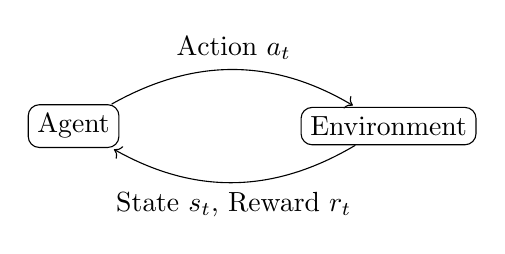
\begin{tikzpicture}[shorten >=1pt,node distance=2cm,on grid,auto] 
   \node[rectangle,draw=black,rounded corners] (q_0)   {Agent}; 
   \node[rectangle,draw=black,rounded corners] (q_1) [right=4cm of q_0] {Environment}; 
    \path[->] 
    (q_0) edge[bend left, above]  node {Action $a_t$} (q_1)
    (q_1) edge[bend left, below]  node  {State $s_t$, Reward $r_t$} (q_0);
\end{tikzpicture}
\caption{Agent-Enviroment interaction loop}
\label{fig:rl loop}
\end{figure}

The main characters are the agent and the environment. At every step, the agent receives a reward and either the 
full state or just an observation of the environment. A state is a complete description of the world, like the 
configuration of a chess game. An observation, though, is a partial description. Imagine an agent in a video 
game: if you don’t have access to the underlying game mechanics, you can only infer information about the world 
through the current frame. The reward indicates how good or bad the agent’s last action was, providing feedback 
about what happened and how the environment might have changed (sometimes the environment changes on its own). 
Based on this, the agent selects its next action, aiming to accumulate as much reward as possible over time, 
known as the return.
\section{Markov Decision Processes}\label{MDP}
The Markov Decision Process (MDP) provides the standard mathematical framework for modelling the interaction 
between an agent and its environment. It serves as a formal model for sequential decision-making under 
uncertainty and is defined as a 5-tuple $(S, A, P_{sa}, \gamma, R)$, where:

\begin{itemize}
    \item $S$ is a set of states
    \item $A$ is a set of actions
    \item $P_{sa}$ are the state transition probabilities. It describes the probability of getting into a state $s_{t+1}$ when being in a state $s_t$ and performing action $a_t$, i.e. $P_{sa}(s_{t+1}|s_t,a_t)$
    \item $\gamma \in [0,1)$ is the discount factor 
    \item R is the reward function. It can depend on the actions and the states, but sometimes also only on the states
\end{itemize}
A defining feature of an MDP is the Markov property, which says that the outcome of an action depends only on 
the current state and not on the prior history of states or actions. Mathematically, this is expressed as:
\begin{equation*}
    P_{sa}(s_{t+1}|s_t,a_t,\dots,s_0,a_0) = P_{sa}(s_{t+1}|s_t,a_t)
\end{equation*}




\section{Terminology}
To understand the key concepts and algorithms of reinforcement learning,
we need to introduce some terminology.

\subsection{Policy}
A policy $\pi$ determines what action an agent should take when it is in a 
particular state. A deterministic policy is defined as $\pi(s) = a$. A stochastic 
policy is defined as $\pi(a|s)$. It tells us what the probability 
is of performing the action $a$ while in state $s$. The probability function here 
is not the same as the state transition probabilities $P_{sa}$!

\subsection{Episodes, Roll-out, Trajectories}
All three represent a sequence of $(s, a, r)$ tuples, where an episode is 
generally from an initial state to a terminal state, a roll-out is from an initial 
or intermediate state to a terminal state, and a trajectory is between any two 
states. But there is no clear distinction in the RL-World  

%\subsection{Horizon}
%The horizon is how far ahead the agent considers rewards.

\subsection{Reward and Return}
The goal of the agent is to maximise some notion of cumulative reward over episodes, given a sequence of 
state action reward tuples $(s_t, a_t, r_t)$. The total \textbf{discounted return} from time step $t$, called $G_t$, is defined as 
\begin{equation*}
    G_t = r_{t+1}+ \gamma r_{t+2} + \gamma^{2} r_{t+3} + \dots = \sum_{k=0}^{\infty} \gamma^{k} r_{t+1+k}
\end{equation*}
The restriction of the discount factor $\gamma$ to the interval $[0, 1)$ is now more evident. Allowing $\gamma = 
1$ in the context of an infinite episode would result in an infinite return $G_t$, which offers little insight 
into the agent's behaviour. For finite episodes, setting $\gamma = 1$ is permissible; however, since we typically
consider the infinite-horizon case, we constrain $\gamma$ to $[0, 1)$. The value of $\gamma$ also significantly 
influences the agent's decision-making. When $\gamma$ approaches 0, the agent behaves ''myopic``, prioritizing 
the maximization of immediate rewards. As $\gamma$ approaches 1, the agent becomes ''farsighted``, placing 
greater emphasis on long-term future rewards.

\subsection{Value Functions}
In order to maximise the return, the agent needs to know which actions to take in each state. Therefore, it is 
often useful to know ''how good'' a particular action performed in a particular state is. The two main functions 
are:
\subsubsection{Value Function}
The state value function $V^{\pi}(s)$ of an MDP is the expected discounted return starting from state s and 
following a policy $\pi$.
\begin{align*}
    V^{\pi}(s) = \mathbb{E}_{\pi}\left[G_t | s_t=s\right] &=  \mathbb{E}_{\pi}\left[\sum_{k=0}^{\infty} 
    \gamma^{k} r_{t+1+k}|s_t=s\right]  \\
     &= \mathbb{E}_{\pi}\left[r_{t+1}+\gamma (r_{t+2}+\gamma r_{t+3} \dots) | s_t=s\right]\\
    &=  \mathbb{E}_{\pi}\left[r_{t+1}+\gamma G_{t+1} | s_t=s\right] \\
    %&=   \mathbb{E}_{\pi}\left[r_{t+1}+\gamma V(s_{t+1}) | s_t=s\right] \\
    &= \sum_a \pi(a|s)\left(R(s,a)+\gamma \sum_{s'} p(s'|s,a)\mathbb{E}_{\pi}\left[G_{t+1}|s_{t+1}= 
    s'\right]\right) \\
     &= \sum_a \pi(a|s)\left(R(s,a)+\gamma \sum_{s'} p(s'|s,a)V^{\pi}(s')\right) \numberthis \label{v bellmann}
\end{align*}
Equation \ref{v bellmann} is called the Bellman equation for $V^{\pi}$.

\subsubsection{Action Value Function}
The action-value function represents the expected return when starting in state $s$, taking action $a$, and 
thereafter following policy $\pi$.
\begin{align*}
    Q^{\pi}(s,a) &=  \mathbb{E}_{\pi}\left[G_t | s_t=s,a_t=a\right]\\
    &=  \mathbb{E}_{\pi}\left[r_{t+1}+ \gamma Q^{\pi}(s_{t+1},a_{t+1}) | s_t=s,a_t=a\right] \\
    &=  R(s,a) + \gamma \sum_{s'}p(s'|s,a)\sum_{a'} \pi(a'|s') \mathbb{E}_{\pi}\left[G_{t+1}|s_{t+1} = s',a_{t+1} 
    = a'\right] \\
    &= R(s,a) + \gamma \sum_{s'}p(s'|s,a)\sum_{a'} \pi(a'|s') Q^{\pi}(s',a') \numberthis \label{q bellmann}
\end{align*}
Equation \ref{q bellmann} is known as the Bellman equation for $Q^{\pi}$. The value function $V$ and the action-
value function $Q$ can also be defined in terms of each other since:
\begin{gather}
    V^{\pi}(s) = Q^{\pi}(s,\pi(s))=\mathbb{E}_{a\sim \pi}[Q^{\pi}(s,a)] \label{eq:v_to_q} \\
    \rightarrow Q^{\pi}(s,a) = R(s,a) + \gamma \sum_{s'}p(s'|s,a)\underbrace{\sum_{a'} \pi(a'|s') Q^{\pi}
    (s',a')}_{V^\pi(s')} \label{eq:q_to_v}%= R(s,a) + \gamma \sum_{s'}p(s'|s,a) V^{\pi}(s')
\end{gather}

\subsubsection{Advantage Function}\label{advantage_function}
In RL, we often care about the relative advantage of an action over some other action rather than the absolute value. 
The advantage function $A^\pi(s,a)$ quantifies how much better taking action $a$ in state $s$ is compared to randomly 
selecting an action according to $\pi(\cdot|s)$ assuming the policy $\pi$ is followed thereafter. Mathematically, 
the advantage function is defined by:
$$A^\pi(s,a) = Q^\pi(s,a)- V^\pi(s)$$
A thing to note is that $\mathbb{E}_{a\sim\pi}[A^\pi(s,a)]=0$ since 
$$\mathbb{E}_{a\sim\pi}[A^\pi(s,a)] = \mathbb{E}_{a\sim\pi}[Q^\pi(s,a)- V^\pi(s)] = 
\mathbb{E}_{a\sim\pi}[Q^\pi(s,a)]- \mathbb{E}_{a\sim\pi}[V^\pi(s)] \overset{\eqref{eq:v_to_q}}{=} V^\pi(s) - V^\pi(s) = 0 
$$
%\footnote{The reason why \( \mathbb{E}_{a \sim \pi}[V^\pi(s)] = V^\pi(s) \) is that \( \mathbb{E}[\mathbb{E}[X]] = \mathbb{E}[X] \), and since \( V^\pi(s) \) is itself an expectation, this holds (\href{https://math.stackexchange.com/questions/2034853/mathematical-expectation-eex-ex}{see}).}

\subsection{Optimisation objective}
As previously noted, the agent's objective is to find a policy that maximizes the return. To achieve this, the 
agent seeks to optimize either the value function or the state-action value function, which then serves as a 
foundation for deriving the policy. The optimal policy is defined as follows:
\begin{gather*}
V^*(s) = \max_{\pi} \mathbb{E}_{\pi}\left[G_t | s_t = s\right] = \max_{a} \left( R(s,a) + \gamma \sum_{s'} 
p(s'|s,a) V^{}(s') \right), \\
Q^*(s,a) = \max_{\pi} \mathbb{E}_{\pi}\left[G_t | s_t = s, a_t = a\right] = R(s,a) + \gamma \sum_{s'} p(s'|s,a) 
\max_{a'} Q^{}(s',a').
\end{gather*}
Given the relationship between the value function and the state-action value function, it follows that $V^*(s) = 
\max\limits_{a} Q^*(s,a)$. With $Q^*$ determined, the optimal policy can be straightforwardly expressed as $\pi^*
(s) = \argmax\limits_{a} Q^*(s,a)$. In the subsequent sections, we will explore algorithms designed to compute 
the optimal policy across various environmental settings.\footnote{ In the literature, the term ''Bellman 
backup`` is sometimes used. It simply refers to the sum of the immediate reward and the value of the next state. 
$Q^{\pi}(s,a) =  \mathbb{E}_{\pi}[\underbrace{r_{t+1}+ \gamma Q^{\pi}(s_{t+1},a_{t+1})}_{\text{Bellman backup}} | 
s_t=s,a_t=a] $}
\section{Optimal decision making via dynamic programming}\label{dynammic programming}
We begin with the simplest scenario, where the agent has full knowledge of the environment, 
including the state transition probabilities and the reward function. A straightforward approach 
to computing the value function for a given policy $\pi$ is the Policy-Evaluation algorithm. 
This method iteratively employs the Bellman equation \eqref{v bellmann} to update and refine the value function.
\begin{algorithm}[H]
   \large
    \caption{Policy Evaluation}\label{policy evaluation}
    \begin{algorithmic}
        \STATE  $V_0^{\pi}(s) \gets 0 $
        \FOR{k = 1 until convergence}
            \FOR{all s in S}
                \STATE $ V_k^{\pi}(s) \gets  \sum_a \pi(a|s)\left(R(s,a)+\gamma \sum_{s'} p(s'|s,a)V_{k-1}^{\pi}(s')\right) $
            \ENDFOR
        \ENDFOR
    \end{algorithmic}
\end{algorithm}
Now we know how to evaluate a policy, but we are interested in finding 
the optimal policy. One naive way is to try every possible policy to find the 
optimal one. But already the number of deterministic policies is $|A|^{|S|}$ 
(because we have in each state $|A|$ possible actions we could take), which is 
intractable. So we use a more efficient algorithm called Policy-Iteration
\eqref{policy iteration}. The idea is to start with a random policy and 
improve it iteratively. 

\hspace{-0.7cm}
\begin{minipage}[t]{0.45\textwidth}
\begin{algorithm}[H]
   \large
    \caption{Policy Iteration}\label{policy iteration}
    \begin{algorithmic}
        \STATE  $\pi_0(s) \gets \text{ randomly for all states s} $
            \WHILE{$\norm{\pi_i-\pi_{i-1}}_1> 0$}
                \STATE $V^{\pi_i} \gets \textbf{ Policy Evaluation} \text{ of } \pi_i$
                \STATE $\pi_{i+1} \gets \textbf{Policy Improvement}$
                \STATE $i+=1$
            \ENDWHILE
    \end{algorithmic}
\end{algorithm}
\end{minipage}
%\hfill
\begin{minipage}[t]{0.55\textwidth}
\begin{algorithm}[H]
  \large
    \caption{Policy Improvement}\label{policy improvement}
    \begin{algorithmic}
        \FOR{s in S and a in A}
        \STATE $Q^{\pi_i}(s,a) \ \gets R(s,a) \ + \gamma \sum_{s'}p(s'|s,a) V^{\pi_i}(s')$
        \ENDFOR
        \FOR{s in S}
        \STATE $\pi_{i+1}(s) = \argmax_{a} Q^{\pi_i}(s,a)$
        \ENDFOR
    \end{algorithmic}
\end{algorithm}
\vspace{0.3cm}
\end{minipage}
It can be shown that this procedure leads to the optimal policy due to its monotonic 
improvement of the policy in every iteration, meaning that $V^{\pi_i}(s) \leq V^{\pi_{i+1}}(s)$.\newline
Another way to find the optimal policy in this setting  is to use the Value-Iteration algorithm 
(\ref{value iteration}). It can also be demonstrated that value iteration converges to an optimal solution. 
\begin{algorithm}[H]
  \large
    \caption{Value Iteration}\label{value iteration}
    \begin{algorithmic}
        \STATE $V_0^{\pi}(s)\gets 0 (\forall s)$
        \WHILE{not converged (for ex. $\norm{V_{k+1}-V_k}> \epsilon $)}
            \FOR{ s in S}
        \STATE $V_{k+1}(s)=\max\limits_{a}\left[R(s,a)+\gamma \sum_{s'}p(s'|s,a)V_k(s')\right]$ \COMMENT{this is equation \eqref{eq:q_to_v}}
        \STATE $\pi_{k+1}(s)=arg \max\limits_{a}\left[R(s,a)+\gamma \sum_{s'}p(s'|s,a)V_k(s')\right]$
            \ENDFOR
        \ENDWHILE
    \end{algorithmic}
\end{algorithm}
The problem with the Policy- and the Value-Iteration algorithm is that they require 
full knowledge of the environment, i.e. dynamics model and reward function. This is often 
not available, so we will now look at methods that allow us to find a optimal policy even 
if we do not have a model of the environment.
\subsection{Self-Test Questions}
\begin{enumerate}
    \sq{The definition of a MDP} $\rightarrow$ \ref{MDP}
    \sq{Why do we need discounting ?} \newline If we would no discount then our 
    return ( discounted future rewards) would be infinite which results in every policy 
    being an optimal policy and making it hard to come up with algorithms to find the 
    optimal policy in these cases. Another thing is that we can control the behaviour of 
    the agent by choosing the the discount factor. If $\gamma \rightarrow  0$ (myopic) 
    then focused on maximizing immediate reward. If $\gamma \rightarrow  1$ (farsighted)
    focused on future rewards.
    
    \sq{The definition of the optimal and the policy based V- and Q-Functions}
    \begin{gather*}
        V^{\pi}(s) = \mathbb{E}[G_t | s_t =s],\;V^*(s)= \max\limits_\pi V^{\pi}(s) \\
        Q^{\pi}(s,a) = \mathbb{E}[G_t | s_t =s,a_t = a],\;Q^*(s,a)= \max\limits_\pi Q^{\pi}(s,a)
    \end{gather*}
    
    \sq{What is the bellman principle of optimality ?}\newline 
   An optimal policy has the property that whatever the initial state and initial 
   decision are, the remaining decisions must constitute an optimal policy with regard 
   to the state resulting from the first decision.
   \begin{gather*}
       V^* (s) = \max\limits_a \left(R(s,a)+\gamma \sum_{s'} p(s'|s,a)V^{*}(s')\right) \\
       Q^*(s,a) = R(s,a) + \gamma \sum_{s'}p(s'|s,a)\max\limits_a Q^{*}(s',a')
   \end{gather*}
    
    \sq{How the value iteration algorithm works} $\rightarrow$ \ref{value iteration}
    
    \sq{How the policy iteration algorithm works} $\rightarrow$ \ref{policy iteration}

    \sq{If in a policy iteration step the policy doesn’t change, can it ever change again? (not from the lecture)}\newline
     No (if $\pi^{*}$ is unique $\forall s$). Because if $\pi_{i}=\pi_{i+1}$ then $ Q^{\pi_i} =  Q^{\pi_{i+1}}$ 
     and this results in the policy never changing again.

     \sq{Is there a maximum number of iterations of policy iteration? (not from the lecture)}\newline
      $|A|^{|S|}$ since that is the maximum number of policies, and as the policy improvement step is monotonically improving, each policy can only appear in one round of policy iteration unless it is an optimal policy.
    
    \sq{What are the conceptual differences between value- and policy-
    iteration? } \newline In policy iteration we first do multiple passes that update 
    the value function and then update the policy with these newly computed values. In 
    value iteration when updating the value function we simultaneously/implicitly also 
    update the policy. Value iteration can be seen as an extreme case of policy 
    iteration where we stop the evaluation after one update.  
    
    \sq{What are the limitations of these approaches ?}\newline
    We must know the dynamics and reward model and it only works for discrete settings or 
    Linear Systems, Quadratic Reward, Gaussian Noise (LQR)
\end{enumerate}
%%%%%%%%%%%%%%%%%%%%%%%%%%%%%%%%%%%%%%%%%%%%%%%%%%%%%%%%%%%%%%%%%%%%%%%%%%%%%%%%%%%%%%%%%%%%%%%%%%%%%%%%%%%%%%%%%%

\section{K-Armed-Bandits}
Before we look at algorithms for the case where we do not have a model of the 
world, we will talk about the k-armed-bandit problem, which helps us to understand decision 
making under uncertainty.\newline
A k-armed bandit is a tuple $(A,p(r|a))$, where $A$ is the known set of $k$ actions we can 
take (arm) and $p(r|a)$ is the unknown probability distribution over rewards. At each time 
step $t$ we take an action $a_t$ and the environment generates a reward $r_t$. The goal is 
to maximise the expected reward. To achieve this goal we have to decide which arm to pull, 
so we need to know the expected reward per action $\hat{q}$ (action value function)
$$ \hat{q}= \mathbb{E}[r_t|a_t=a] = \int p(r|a) r \;\texttt{d}r$$
Since we do not know $p(r|a)$, we approximate the integral by Monte Carlo simulation. 
$$\hat{q}= \mathbb{E}[r_t|a_t=a] \approx \frac{\sum_{i=1}^{t-1} \mathds{1}(a_i=a)r}
{\sum_{i=1}^{t-1} \mathds{1}(a_i=a)} = q_t(a)$$
Instead of storing all the rewards to calculate the sum, one can also reformulate 
it using an incremental update rule.
\begin{align*}
    q_{n+1} = \frac{1}{n}\sum_{i=1}^n r_i &= \frac{1}{n} \left(r_n+ \sum_{i=1}^{n-1} r_i \right) \\
    &= \frac{1}{n} \left(r_n+ (n-1){\color{blue}\frac{1}{n-1}\sum_{i=1}^{n-1} r_i} \right) \\
    &=  \frac{1}{n} \left(r_n+ (n-1){\color{blue}q_n} \right)\\
    &= q_n + \frac{1}{n}(r_n-q_n) \numberthis \label{eq:running_avg}
\end{align*}
This formulation is called the sampled average method, whereas the more general update rule looks like this.
$$q_{n+1} = q_n + \alpha_n (r_n-q_n)$$
We will now consider different strategies for choosing actions to maximise the expected 
reward.
\subsection{Greedy action selection}
In greedy action selection, our next action $a_t$ is defined as $$a_t = \argmax\limits_{a\in 
A} q_t(a)$$ The problem with this approach is that we could get stuck in a suboptimal 
policy. Consider the following example where we have three actions $a_1,a_2,a_3$ to choose 
from with unknown true rewards ${q(a_1)=0.95,q(a_2)=0.9,q(a_3)=0.1}$. We know have as the 
initial q-values the values \newline ${q(a_1)= q(a_3) = 0,q(a_2)=1}$. From there on we do 
greedy action selection, which results in only picking the action $a_2$ even though the 
actual best action to take is $a_1$, but for that we would have to drift from our strategy. 
This is the core problem in RL. We need to make a trade-off between Exploration: Improve 
knowledge for long term benefit and Exploitation: Using knowledge for short-term benefit. 
One way to achieve this is called $\epsilon$-greedy exploration, 
where we choose a value $\epsilon \in [0,1]$ representing the probability of 
exploring/exploiting.
$$ a = \left\{
\begin{array}{ll}
\argmax_a q_t(a) & \text{with probability } 1-\epsilon \\
\text{Uniform}({a_1,\dots,a_k}) & \, \text{with probability } \epsilon\\
\end{array}
\right.$$

\subsection{Exploration and Entropy}
Although $\epsilon$ greedy action selection is an effective means of balancing exploration 
and exploitation in reinforcement learning, one 
drawback is that when it explores, it chooses equally among all actions. 
This means that it is just as likely to choose the worst appearing 
action as it does the next best action. In tasks where the worst actions are very bad, this 
can be unsatisfactory. The obvious solution is to vary the action probabilities as a  
graded function of the estimated value (exploitation). But at the same time, we are 
uncertain about the rewards and therefore need to keep uncertainty in the policy, for which 
entropy is a good measure (exploration). Thus the objective looks like this 
\begin{align*}
    \pi^*_t = \argmax\limits_\pi \sum_a \pi(a) q_t(a) + \tau^{-1}H(\pi) &=\argmax\limits_\pi \sum_a \pi(a) q_t(a) + \tau^{-1} (- \sum_a \pi(a)\log{\pi(a)})\\   &=\argmax\limits_\pi \sum_a \pi(a)(q_t(a)-\tau^{-1}\log{\pi(a)})
\end{align*}
Calculation the derivative and setting it equal to zero gives us the policy which maximises the objective $$ \pi(a)= \frac{\exp(\tau q_t(a))}{\sum_{a'}\exp(\tau q_t(a'))}$$

\subsection{Optimistic Value Initialization}
The idea is simply to initialise the q-values with optimistic values, this has the effect of 
adding a positive bias to less explored actions, thus forcing exploration.

\subsection{Upper-Confidence-Bounds (UCB)}\label{UCB}
The UCB formula is defined as $$ a_t = \argmax\limits_a 
\underbrace{q_t(a)}_{\text{exploitation}} + \underbrace{c \sqrt{\frac{\log{t}}
{N_t(a)}}}_{\text{exploration}}$$
$c$ is a constant that allows us to set the exploration/exploitation trade-off. 
$\sqrt{1/{N_t(a)}}$ essentially says that the more times you pull an arm, there is less unknown about that arm. 
So the fewer times action a is chosen, the higher the exploration bonus.
$\sqrt{\log{t}}$ ensures that you don't stop exploring too early. \newline 
In the following, we will examine how different strategies perform across various parameter settings. 
To do this, we utilize a 10-armed bandit experiment, averaging the results over 2000 runs with sample 
average action-value estimates.

\begin{figure}[H]
    \centering
    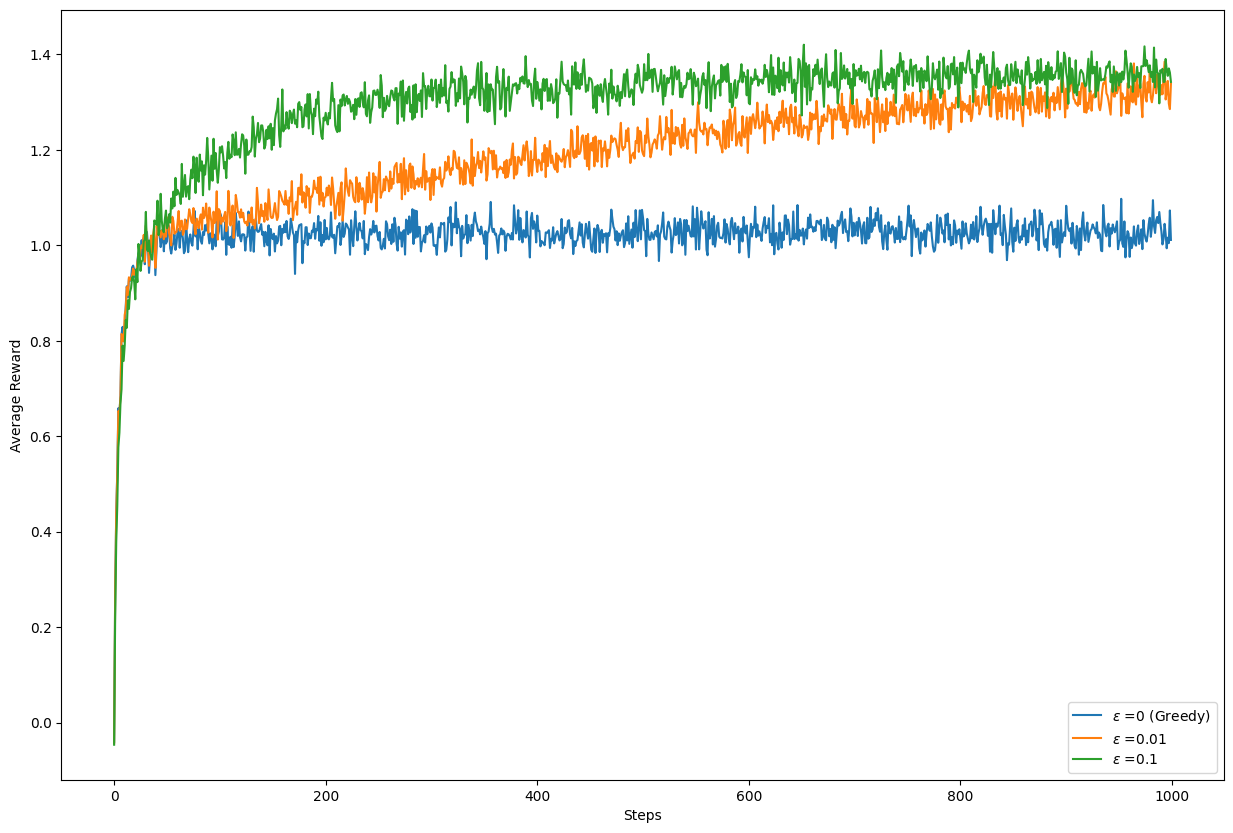
\includegraphics[width=\linewidth, height=0.33\textheight]{images/bandit_greedy.png}
    \caption{$\epsilon$-Greedy}
\end{figure}

\begin{figure}[H]
\vspace{-1.5cm}
    \centering
   \begin{minipage}{\linewidth}
        \centering
        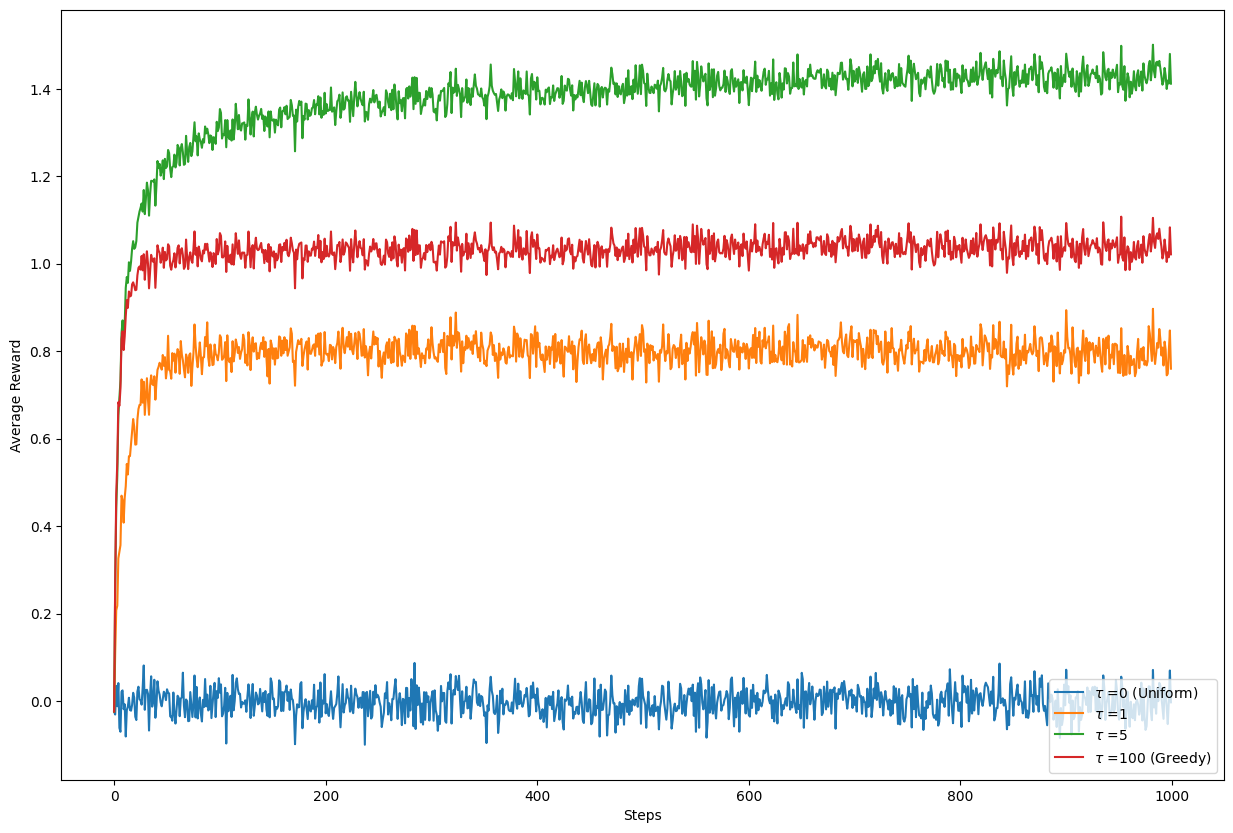
\includegraphics[width=\linewidth, height=0.33\textheight]{images/bandit_softmax.png}
        \caption{Softmax}
    \end{minipage}
    
    
    \vspace{0.5mm} % Small spacing between minipages
    
     \begin{minipage}{\linewidth}
        \centering
        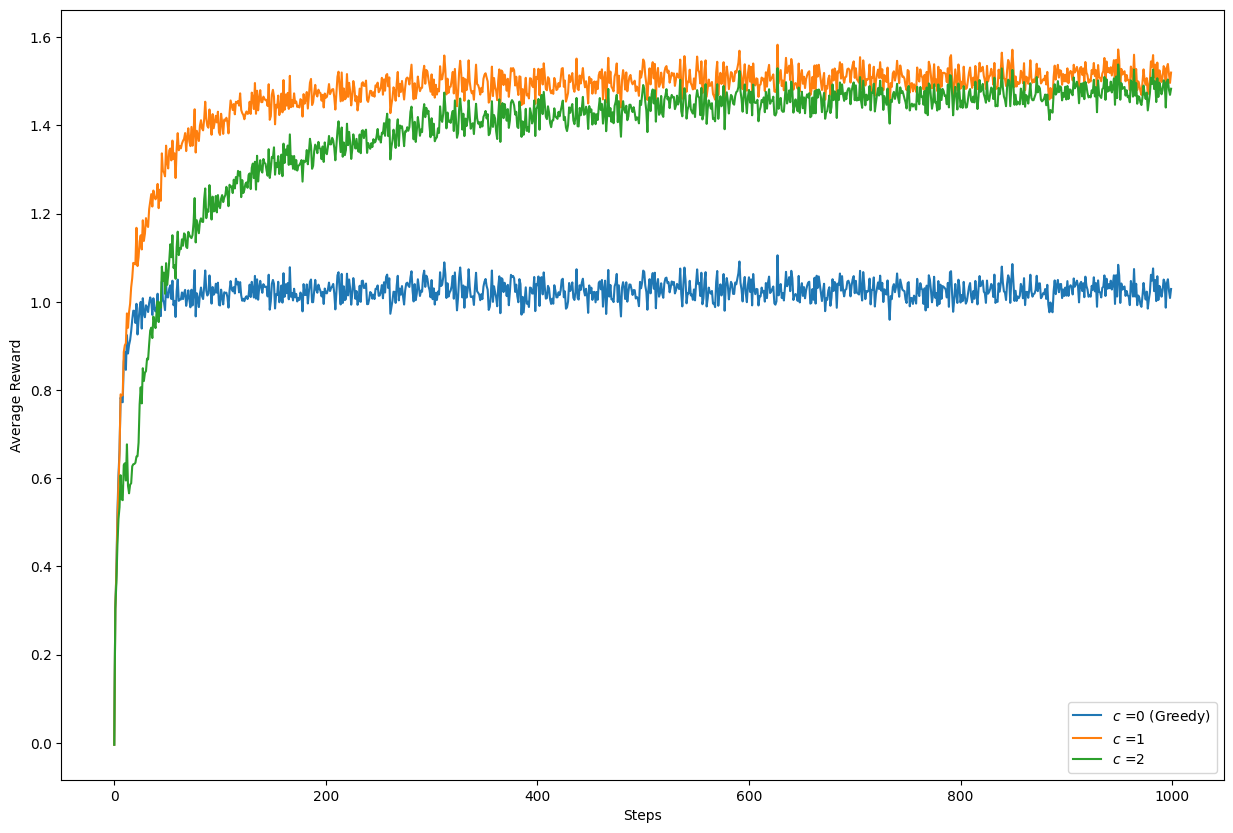
\includegraphics[width=\linewidth, height=0.33\textheight]{images/bandit_ucb.png}
        \caption{UCB}
    \end{minipage}
    
    
    \vspace{0.5mm}
    
    \begin{minipage}{\linewidth}
        \centering
     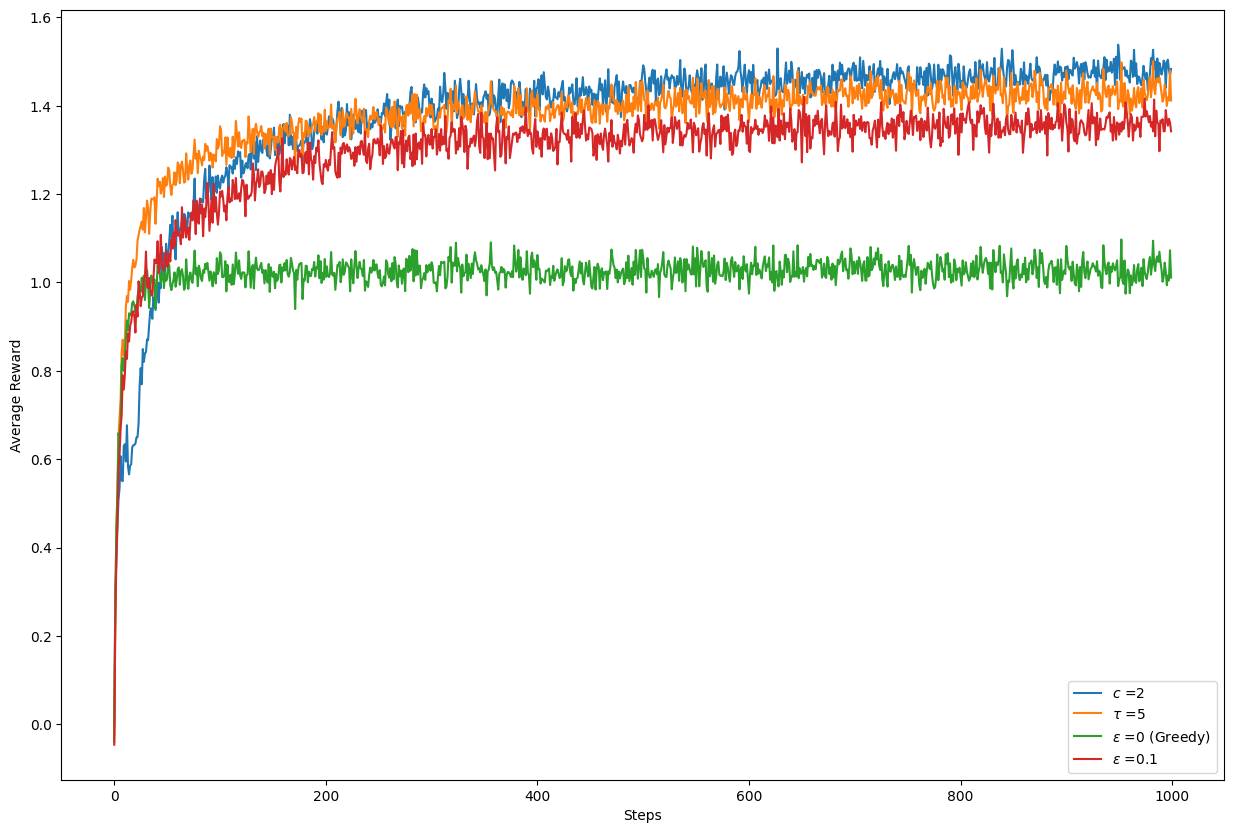
\includegraphics[width=\linewidth, height=0.33\textheight]{images/bandit_comparison.png}
    \caption{Comparison of different strategies}
    \end{minipage}
    
    \label{fig:three-methods}
\end{figure}
\section{Temporal Difference (TD)- Methods}\label{section:td-methods}
We now shift to the setting where we lack a model of the environment from which to derive 
an optimal policy. Instead, we are provided with sample trajectories, denoted as 
$\tau = (s_0, a_0, r_0, s_1, a_1, r_1, \dots)$, and must learn from these directly.

\subsection{Monte Carlo policy evaluation}\label{Monte Carlo policy evaluation}
Recall that the value function under a policy $\pi$ is defined as 
$V^{\pi}(s) = \mathbb{E}_{\pi}\left[G_t \mid s_t = s\right]$, where $G_t$ represents 
the discounted return starting from state $s$ at time $t$. The idea of Monte Carlo policy evaluation
is to approximate this expectation using Monte Carlo simulation. The core idea of Monte 
Carlo methods is to estimate an expectation, $\mathbb{E}_{p(x)}\left[f(x)\right] = \int p(x) f(x) \; dx$, 
by sampling from the distribution and averaging the results:
$$\mathbb{E}_{p(x)}\left[f(x)\right] = \int p(s)f(x) dx \approx \frac{1}{N} 
\sum_{x_i \sim p(x)} f(x_i)$$
This translates to sampling random episodes or trajectories under the policy $\pi$ 
and averaging the returns observed for each state to approximate $V^{\pi}(s)$. 
There are two primary approaches to compute this estimate: First-Visit Monte Carlo and Every-Visit Monte Carlo.
These methods differ in how they handle state visits within an episode and update the value estimates. 
The First-Visit approach updates the estimate only the first time a state $s$ is encountered at a timestep $t$ 
in an episode. In contrast, the Every-Visit approach updates the estimate for every occurrence of a 
state across all timesteps in the episode. At their core, they work as follows:

\begin{algorithm}[H]
  \large
    \caption{Monte Carlo Policy Evaluation }\label{MCPE}
    \begin{algorithmic}
        \STATE $N(s)\gets 0, G(s)\gets 0 \; \forall s \in S$
        \FOR{}
        \STATE sample episode $i = s_{i,1},a_{i,1},r_{i,1},s_{i,2},a_{i,2},r_{i,2},\dots,s_{i,T_i},a_{i,T_i},r_{i,T_i}$ \vskip 5pt
        \STATE define $G_{i,t} = r_{i,t}+ \gamma  r_{i,t+1} + \gamma^2  r_{i,t+2} + \dots +  \gamma^{T_i -1}  r_{i,T_i} $ as the return from time step $t$ onwords in the $i$th episode \vskip 5pt
        \FOR{$t \in T_i$} \vskip 3pt

        \STATE \tikzmk{A} \textcolor{red}{First-Visit Monte Carlo} 
        \STATE \textbf{if} this is the first time t that state s is visited in episode i
        \STATE
        \tikzmk{B}\boxit{mypink} 
        \STATE \tikzmk{A} \textcolor{blue}{Every-Visit Monte Carlo}
        \STATE state $s$ is being visited at time step $t$ in episode $i$
        \STATE
        \tikzmk{B}\boxit{myblue}
        \STATE increment counter of total visits $N(s) = N(s)+1$
        \STATE  $V^{\pi}(s)= V^{\pi}(s) + \alpha(G_{i,t}- V^{\pi}(s))$ \COMMENT{for $\alpha = \frac{1}{N(s)}$ equal to running average see \eqref{eq:running_avg}}
        
        %\STATE \tikzmk{A} \textcolor{red}{First-Visit Monte Carlo} 
        %\IF{this is the first time t that state s is visited in episode i}
        %\STATE increment counter of total first visits : $N(s)= N(s)+1$
        %\STATE increment total return $G(s) = G(s)+ G_{i,t}$
        %\STATE update estimate $V^{\pi}(s)= G(s)/N(s)$
        %\ENDIF
        %\STATE
        %\tikzmk{B}\boxit{mypink} 
        
        %\STATE \tikzmk{A} \textcolor{blue}{Every-Visit Monte Carlo}
        %\STATE state $s$ is being visited at time step $t$ in episode $i$
        %\STATE increment counter of total visits $N(s) = N(s)+1$
        %\STATE increment total return $G(s) = G(s)+ G_{i,t}$
        %\STATE update estimate $V^{\pi}(s)= G(s)/N(s)$
        %\STATE
        %\tikzmk{B}\boxit{myblue}
        
        %\STATE \tikzmk{A} \textcolor{black!70!green}{Incremental Monte Carlo}
        %\STATE state $s$ is being visited at time step $t$ in episode $i$
        %\STATE increment counter of total visits $N(s) = N(s)+1$
        %\STATE  $V^{\pi}(s)= V^{\pi}(s) + \alpha(G_{i,t}- V^{\pi}(s))$
        %\STATE
        %\tikzmk{B}\boxit{mygreen}
        \ENDFOR
        \ENDFOR

    \end{algorithmic}
\end{algorithm}
Convergence can be guaranteed depending on the choice of $\alpha$, provided the 
following conditions are satisfied:
\begin{itemize}
\item $\sum_{n=1}^{\infty} \alpha_n(s,a) = \infty \;\forall (s,a)$
\item $\sum_{n=1}^{\infty} \alpha_n^2(s,a) < \infty \;\forall (s,a)$            
\end{itemize}
The sample average method, using $\alpha_n = \frac{1}{n}$, fulfills these requirements. 
Additionally, it’s worth noting that the First-Visit Monte Carlo method is an unbiased 
estimator, whereas the Every-Visit Monte Carlo method is both unbiased and consistent
(meaning $\forall \epsilon > 0: \lim\limits_{n\rightarrow\infty} P(|V_n^{\pi}-V|> \epsilon)= 0$).\newline
The problem with the Monte Carlo estimator is that it is a high variance estimator, because if the 
policy or the environment is highly stochastic, the total return $G_t$ from a state can vary a lot 
even if you start from the same state. So, you're 
averaging a bunch of noisy, random returns = variance.
Reducing the variance can require a lot of data. Therefore, in cases where data is 
expensive to obtain MC may be impractical. Another 
disadvantage is that it only works if we have an episodic setting, which makes it 
very sample inefficient because we have to wait for the whole episode to end before we can 
compute the returns. But a nice feature is that it does not require the model to be 
Markov.

\subsection{Temporal Difference Learning}
Temporal Difference (TD) Learning combines the Monte Carlo method with dynamic programming 
which is used in the Value- and Policy-Iteration algorithms. This model-free technique is applicable
to both episodic and non-episodic environments. It updates the value function $V$ immediately after
each transition tuple $(s, a, r, s')$, with an update rule resembling that of incremental 
Monte Carlo methods:
$$V^{\pi}(s)= V^{\pi}(s) + \alpha(\underbrace{[r+ \gamma V^{\pi}(s')]}_{\text{TD target}}- V^{\pi}(s))$$
This version is known as TD(0), as it uses a one-step lookahead/ one-step return—for updating the value estimates.
\vspace{-0.2cm}
\begin{algorithm}[H]
 % \large
    \caption{Temporal Difference (TD(0)) Learning Algorithm }\label{TD_learning_algo}
    \begin{algorithmic}
        \STATE $V_0^{\pi}(s)\gets 0, \forall s \in S$
        \STATE Loop for each episode:
        \STATE \quad init. s
        \STATE \quad Loop 
        \STATE \qquad sample tuple $(s,a,r,s')$ from $\pi$
        \STATE \qquad $V^{\pi}(s)= V^{\pi}(s) + \alpha(r+ \gamma V^{\pi}(s'))- 
        V^{\pi}(s))$
        \STATE \qquad $s \gets s'$
        \STATE \quad until s is terminal
    \end{algorithmic}
\end{algorithm}
A key limitation of this approach is its inability to directly support policy improvement 
(see algo. \ref{policy improvement}). To compute the Q-values, we rely on the dynamics model, 
but such a model is unavailable in a model-free setting:
$$Q^{\pi_i}(s,a) \ \gets R(s,a) \ + \gamma \sum_{s'}{\color{red}p(s'|s,a)} V^{\pi_i}(s')$$
To address this, we shift to learning the Q-function directly instead of the value function, 
enabling policy improvement without dependence on the dynamics model.
%Recall that the goal is to choose actions that maximise expected future reward. But 
%n order to do this, we need to try out actions in order to know if they are 
%beneficial or not. This trade off of exploration vs exploitation has been already 
%addressed in k-armed-bandit chapter. With the following algorithms we will see how 
%this idea also plays a role.  

\subsection{Generalized Policy Improvement}
The first algorithm we’ll look at is Monte Carlo Online Control, which builds on 
Monte Carlo Policy Evaluation by incorporating updates to the Q-values.
\begin{algorithm}[H]
  %\large
    \caption{Monte Carlo Online Control}\label{Monte Carlo online control}
    \begin{algorithmic}
        \STATE $N(s,a)\gets 0, Q(s,a)\gets 0 \; \forall (s,a) \in S \times A$
        %\STATE $\epsilon \gets 1, k \gets 1$
        \FOR{(over episodes)}
        \STATE sample episode $i = s_{i,1},a_{i,1},r_{i,1},s_{i,2},a_{i,2},r_{i,2},\dots,s_{i,T_i},a_{i,T_i},r_{i,T_i}$ according to $\pi$ 
        \STATE define $G_{i,t} = r_{i,t}+ \gamma  r_{i,t+1} + \gamma^2  r_{i,t+2} + \dots +  \gamma^{T_i -1}  r_{i,T_i} $ 
        %as the return from time step $t$ onwords in the $i$th episode 
        \FOR{$t \in T_i$}
        \IF{First-Visit // Every-Visit}
        \STATE $N(s,a)= N(s,a)+1$
        \STATE $Q(s,a) = Q(s,a)+ \frac{1}{N(s,a)}(G_{i,t}-Q(s,a))$
        \STATE $\pi(s) \gets \argmax\limits_{a'} Q(s,a')$
        \ENDIF
        \ENDFOR
        %\STATE $k\gets k+1,$
        %\STATE $\epsilon \gets \frac{1}{k}$
        \ENDFOR
    \end{algorithmic}
\end{algorithm}
The Monte Carlo Online Control algorithm \footnote{ Monte Carlo Online Control isn’t sourced from the KIT lecture; it think i got it from Stanford’s CS234 course, so feel free to skip it.} converges to the optimal state-action 
value function $Q^*$ if the two conditions are fulfilled:
\begin{itemize}
\item Every state-action pair $(s, a)$ is visited infinitely often, expressed as
$\lim\limits_{i \to \infty} N_i(s, a) \to \infty$.
\item The behavior policy (the policy guiding actions in the environment) converges
to a greedy policy with probability 1, i.e., $\lim\limits_{i \to \infty} \pi(a|s) \to \arg\max_a Q(s, a)$.
\end{itemize}
These conditions are sometimes referred to as the ''Greedy in the Limit with Infinite Exploration``
(GLIE \label{glie}) property.

\subsubsection{TD-Learning with Q-Values}\label{sarsa and q learning}
Next, we will examine two variants of Temporal Difference (TD) Learning that update 
Q-values rather than value functions: SARSA and Q-Learning. While these methods are 
nearly identical, they only differ in their Q-value update rules.\newline
We begin with SARSA, the on-policy variant. In SARSA, the next action used to compute
the Q-value is determined by the current policy.
\begin{algorithm}[H]
  \large
    \caption{SARSA (on-policy TD control)}\label{Sarsa}
    \begin{algorithmic}
        \STATE $Q(s,a)\gets 0, \forall (s,a) \in S \times A$
        \STATE Loop for each episode:
        \STATE \quad init. s
        \STATE \quad choose a from s using policy derived from Q(e.g., $\epsilon-$greedy)
        \STATE \quad Loop for each step of episode
        \STATE \qquad take action $a$, observe $r,s'$ 
        \STATE \qquad choose $a'$ from $s'$ using policy derived from Q(e.g., $\epsilon-$greedy)
        \STATE \qquad $Q(s,a) \gets Q(s,a) + \alpha[r+\gamma Q(s',a')-Q(s,a)] $
        \STATE \qquad $s \gets s',a \gets a'$
        \STATE \quad until s is terminal
    \end{algorithmic}
\end{algorithm}
Q-Learning closely resembles SARSA, but operates off-policy due to the difference in 
its Q-value update rule:
$$Q(s,a) \gets Q(s,a) + \alpha[r+\gamma \;{\color{red}\max\limits_{a'}}\;Q(s',a')-Q(s,a)] $$
The $\max$ operator is what makes Q-Learning off-policy. Rather than sticking to the current 
policy to select the next action, it greedily chooses the action with the highest Q-value, 
diverging from the policy being followed. Both SARSA and Q-Learning can converge to the optimal solutions 
provided they satisfy the GLIE condition (see \ref{glie}) and the step sizes $\alpha_t$ meet the following two
criteria:
\begin{itemize}\label{robbins munro}
\item $\sum_{n=1}^{\infty} \alpha_n(s,a) = \infty \;\forall (s,a)$
\item $\sum_{n=1}^{\infty} (\alpha_n(s,a))^2 < \infty \;\forall (s,a)$
\end{itemize}
But there is still a problem with the algorithms shown here. They only work when
we can store all the values in tables. In fact, every algorithm so far only works if 
we can store the values in tables. For systems with many states and actions, this is 
a computational burden. And also the conditions for GLIE are somewhat impossible to 
fulfil if we have too many states and actions. Instead, we want a more compact 
representation that generalises across states or states and actions.

\subsection{Function Approximation for policy evaluation}
Rather than relying on tabular representations, we now use parametrized Q or V functions.
These can range from simple linear models to complex neural networks. The algorithms introduced
earlier remain mostly unchanged, except that we now also train a function approximator. 
Since the true Q-, V- or Reward-Function values are unavailable during training, we rely on approximated
targets as labels. The most well-known function approximation algorithm is
the Deep Q-Learning (DQN) algorithm, defined as follows:
 \begin{algorithm}[H]
  \large
    \caption{Vanilla Deep-Q-Learning (DQN)}\label{vanilla_dqn}
    \begin{algorithmic}
    \STATE \textbf{Input} $\alpha$
    \STATE $\text{init } \omega , t = 0$
    \STATE init. s
    \STATE \textbf{Loop} for each episode:
    \STATE \quad choose a from s using policy derived from $Q_\omega(s,a)$
    \STATE \quad observe $r,s'$ 
    \STATE \quad $y_i = \left\{
\begin{array}{ll}
r & \text{episode terminated at step i+1} \\
r + \gamma \max\limits_{a'}Q_\omega(s',a') & \, \textrm{otherwise} \\
\end{array}
\right. $
    \STATE \quad Do gradient descent step on $(y_i- Q_\omega(s,a))^2$ 
    \STATE \quad  $\omega \gets \omega + \alpha (y_i -  Q_\omega(s,a))\nabla_\omega  Q_{\omega}(s,a)$
    \STATE \quad $t \gets t+1$
    \STATE \quad $s \gets s'$
    \STATE \textbf{end loop}
    \end{algorithmic}
\end{algorithm}
One might argue that the gradient calculation of the loss contains an error, 
as $y_i$ also depends on $w$, yet its derivative seems to be missing. This is intentional.
The update rule incorporating the full gradient is known as the ''Residual Gradient Algorithm``. 
However, this approach minimizes the mean squared temporal difference error (MSTD), defined as:
$$ \text{MSTD} = \mathbb{E}_\pi\left[\left(r_t+\gamma \max\limits_{a'}Q_\omega(s',a')-Q_\omega(s, a)
\right)^2\right] \label{MSTD}$$ Minimizing the MSTD, however, does not guarantee Bellman optimality. 
Furthermore, the bias inherent in the residual gradient algorithm often results in 
suboptimal performance and slow convergence, making it less used in practice.\newline
An alternative approach to achieve Bellman optimality involves minimizing the Mean Squared 
Bellman Error (MSBE), defined as:
$$\text{MSBE} = \mathbb{E}_\pi\left[\left(r_t+ \gamma\mathbb{E}_{\color{red}p(\cdot|s, 
a)}[\max\limits_{a'}Q_\omega(s',a')]-Q_\omega(s,a)\right)^2\right] \label{MSBE}$$
However, computing the inner expectation in this formulation requires knowledge of the transition model,
which poses a significant challenge in the model free setting. One could simply use a single sample to 
estimate the expectation, which would effectively reduce the MSBE to the MSTD. However, there are also 
methods that employ two samples to address this, known as the double sampling approach. 
But these will not be discussed further.\newline Most of the time people will use the MSTD but don't take the gradient of 
the target values.

\subsubsection{Max Action Calculation}
To calculate the targets, we need to identify the action $a'$ with the highest Q-value for a given state. 
In discrete settings, the typical approach is to evaluate all possible actions and select the best one. 
However, this becomes highly inefficient and impractical for high-dimensional or continuous action spaces. 
There are several strategies to address this challenge, which we will explore in later chapters. Some of these include:

\begin{itemize}
    \item Gradient optimization on the Q-value network: One approach is to optimize the Q-value 
    network directly to find the best action. However, this introduces an additional inner loop 
    alongside the existing loop, which can significantly slow down the algorithm.
    
    \item Random shooting: This method involves sampling a set of actions $( a_1, \dots, a_n )$ 
    (e.g., uniformly), and selecting the best action from this set to maximize the Q-value when 
    calculating the target. While this approach is valid, it does not guarantee optimal results.
    
    \item Iterative stochastic optimization: This category includes methods such as the Cross-Entropy Method (CEM),
    Covariance Matrix Adaptation Evolution Strategy (CMA-ES), and others. These techniques operate similarly to random
    shooting but improve upon it by iteratively refining the action selection process to converge toward the optimal action. 
    (See Chapter~\ref{evo_strats} for more details.)

    \item Learning an approximate maximizer with a neural network: In this approach, a neural 
    network $ \mu_\beta $ is trained to approximate the action that maximizes the Q-value, i.e., 
    $ \mu_\beta \approx \argmax\limits_a Q_\psi(s,a) $.
\end{itemize}

\subsubsection{Improving DQN}
The vanilla DQN algorithm, as we have seen in algorithm \ref{vanilla_dqn}, is known to diverge 
very easily. There are two main problems. The first is that sequential states are 
highly correlated because some of the time steps are dependent on each other. The Q function would be 
updated many times for similar states while forgetting the Q values for other states 
(called catastrophic forgetting). In the DQN paper, they used a biologically 
inspired mechanism called experience replay (replay buffer). This approach stores past experiences and 
randomly samples mini-batches from the buffer during training, removing correlations in the observation sequence.\newline
The second challenge arises because the targets ($y_i$) are computed using the same model which is being trained. 
With each update, the target values shift alongside the Q-function, making the training process unstable. The solution is
to use a separate set of older weights to calculate the target values.
%A common choice for updating the target parameters is something similar to polynomial averaging.
%$$\omega' = \tau \omega'+(1-\tau)\omega$$

 \begin{algorithm}[H]
  \large
    \caption{Deep-Q-Learning (DQN) with Replay-Buffer and Target Networks \cite{mnih2013playingatarideepreinforcement}}\label{dqn}
    \begin{algorithmic}
    \STATE \textbf{Input} C,$\alpha,\tau$
    \STATE ${\color{cyan}D \gets \{\}}, \text{init } \omega, {\color{cyan}\omega'=\omega}, t = 0$
    \STATE init. s
    \STATE \textbf{Loop} for each episode:
    \STATE \quad choose a from s using policy derived from $Q_\omega(s,a)$
    \STATE \quad observe $r,s'$ 
    \STATE \quad {\color{cyan} store transition $(s,a,r,s')$ in replay buffer $D$}
    \STATE \quad {\color{cyan}sample random minibatch of tuples $(s_t,a_t,r_t,s_{t+1})$ from D}
    \STATE \quad \textbf{for} $i$ in minibatch \textbf{do} 
    \STATE \qquad $y_i = \left\{
\begin{array}{ll}
r_i & s_{i+1} \text{ is terminal} \\
r_i + \gamma \max\limits_{a'}Q_{\color{cyan}\omega'}(s_{i+1},a') & \, \textrm{otherwise} \\
\end{array}
\right. $
    \STATE \qquad Do gradient descent step on $(y_i- Q_\omega(s_i,a_i))^2$ for parameters
    \STATE \qquad  $w: \Delta w = \alpha (y_i -  Q_\omega(s_i,a_i))\nabla_\omega  Q_\omega(s_i,a_i) $
    \STATE \quad \textbf{endfor}
    \STATE \quad \textbf{if }$mod(t,C) == 0$ \textbf{then}
    \STATE \qquad {$\color{cyan}\omega' \gets \tau \omega'+(1-\tau)\omega $}
    \STATE \quad \textbf{endif}
    \STATE \textbf{end loop}
    \end{algorithmic}
\end{algorithm}

\subsubsection{Double Deep Q Learning}
The modified DQN algorithm works very well, but there is still a problem with this approach.
The issue is that the Q-values are overestimated, as depicted in Figure \ref{fig:ddqn}.
The problem lies in the max/argmax operator used for calculating the target values.
$$y_i= r_i + \gamma\;{\color{red}\max\limits_{a'}}\;Q_{\omega'}(s_{i+1},a') 
=  r_i + \gamma \;Q_{\omega'}(s_{i+1},{\color{red}\argmax\limits_{a'}}\;Q_{\omega'}(s_{i+1},a'))$$
The max operator is biased under noise, leading to overestimation. For random variables, this implies:
$$\mathbb{E}[\max{(X_1,X_2,\dots)}] \geq \max{(\mathbb{E}[X_1],\mathbb{E}[X_2],\dots)}$$
To understand this intuitively, imagine trying to determine the heaviest person in a group where everyone 
has the same true weight (e.g., 70kg), but the scale introduces random noise of $\pm$1kg. If you take the maximum
of these noisy measurements, it will almost always be greater than 70kg. Thus, the expectation of the maximum exceeds 
the maximum of the expectations, resulting in an upward bias.\newline 
Since the Q-values we use are estimates and inherently noisy, this max-based target leads to systematic overestimation during 
training. The solution is to use two different networks for action selection and value computation, i.e. the current network 
$\omega$ and the target network $\omega'$.
$$y_i = r + \gamma Q_{\beta}(s',\argmax\limits_{a'}\; Q_{\alpha}(s',a'))$$. 
\begin{figure}[H]
    \centering
    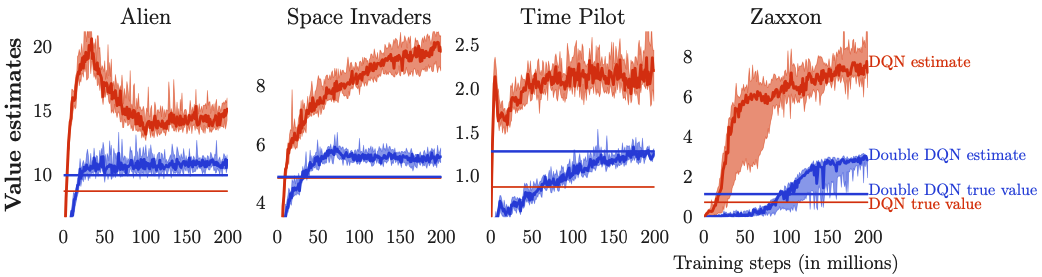
\includegraphics[width=\linewidth]{images/DDQN.png}
    \caption{Value estimates by DQN (orange) and Double DQN (blue) on some Atari games, from \cite{vanhasselt2015deepreinforcementlearningdouble}}
    \label{fig:ddqn}
\end{figure}

\subsubsection{Multi-Step Returns} \label{multi_steps}
In the versions of Q-Learning /DQN we've been looking at, a 1-step look-ahead is employed to compute the targets 
$$y = r + \gamma \max\limits_{a'}Q_\omega(s',a')$$
This results in low variance but a high bias, suggesting that the Q is likely 
wrong. \newline 
To address this, we can use n-step returns, which extend the target by rolling out the actual rewards over $n$
steps before bootstrapping from the Q-function:
$$y_t = r(s_t,a_t)+ \gamma r(s_{t+1},a_{t+1})+ \gamma^2  r(s_{t+2},a_{t+2})+\dots+\gamma^n\max\limits_{a'}Q_\omega(s_{t+n},a')$$
Conversely, an n-step look-ahead yields no bias but high variance. Therefore,
a trade-off has to be made. But n-step returns are not compatible with off-policy methods such 
as Q-learning, as it violates the definition of the Q-function, which is defined as 
the expected sum of future rewards if we start in state s and perform action a and 
then follow the policy. In the context of a two-step look-ahead, the target is defined as
$$y_t = r(s_t,a_t)+ \gamma r(s_{t+1},a_{t+1})+\gamma^2\max\limits_{a'}Q_\omega(s_{t+2},a')$$
Note that $s_t$ and $a_t$ may take on any value since their choice does not violate 
the definition. But it is necessary for $a_{t+1}$ to align with the policy in order 
to ensure that the condition is met. This, however, implies that the choice of 
$a_{t+1}$ is not entirely free, and consequently, the look a head is not off-policy. 
It is noteworthy that there exist multiple methods to circumvent this issue, which 
will not be delved into in this discussion.
%Finally, I would encourage you to look at the rainbow paper, which is a gateway to all sorts of dance techniques.

\subsection{Self-Test Questions}
 \begin{enumerate}
     
\sq{ What we mean by Monte Carlo estimates} $\rightarrow$ \ref{Monte Carlo policy evaluation}

\sq{ Why TD learning can be seen as a combination of MC and Dynamic 
Programming}\newline DP because we compute the value function iteratively starting 
from 0 for all states and MC because we sample an action in every iteration and use 
that action to compute the target $y_t$ for time step $t$. This target is then 
incorporated by moving average 

\sq{ What is the TD error ? }$V^{\pi}(s_t)= V^{\pi}(s_t) + \alpha 
\underbrace{([r_t+ \gamma V^{\pi}(s_{t+1})]- V^{\pi}(s_t))}_{\text{TD error}}$

\sq{ How Q-Learning works} $\rightarrow$ \ref{sarsa and q learning}

\sq{ What Value function approximation is}\newline We don't store the values in tables 
any more. Instead, we use parametrised function approximations of the V/Q-Function. 
Here we calculate the gradients of specific loss functions in order to update the parameters. 

\sq{ Why Q-Learning is not actual gradient ascent?} \newline There is no clearly defined 
objective since the targets are always changing since we also approximate them ourself.

\sq{ How to fix Q-learning for deep neural networks?}\newline
Use a replay buffer where we randomly select transitions to solve the problem that 
successive states are highly correlated. And use a separate target network to 
compute the targets to solve the problem that the targets would keep changing 
because they were computed by the same network that was supposed to learn the policy.

\sq{ Why do we get the over-estimation effect and how to fix it?}\newline
Under noise the max operator is biased to be larger than it should be. And since our 
estimate of Q is a noisy estimate this leads to the overestimation effect. We fix it by 
using the double DQN method. There we use two separate networks. The first one selects the 
(what it thinks) best possible action and the second one calculates the target by using the 
suggested action.

\end{enumerate}

\subsection{Resources}
Much of the content here on Deep Q-Learning is based on Sergey Levine’s CS 285: Lecture 8 \cite{CS285,CS285LevineYoutube}.
\section{Policy Gradients} \label{PG}
In this section we change the approach to finding the optimal policy. The previous 
approaches were designed to approximate the value or action value function, which 
was then used to generate a policy. But there are some difficulties with this 
approach. In order to derive a policy from the value 
function, we would need the dynamics model. By learning the q-value we are able to 
derive a policy, but this also becomes more challenging to solve efficiently for 
high dimensional/continuous action spaces. With policy gradients we parametrise the 
policy $\pi_{\theta}$ directly, where the goal is to find the optimal parameter 
$\theta$ in order to maximise the value function.\newline 
%The policies will be stochastic rather than deterministic, and we will also be 
%focusing on the finite horizon setting, so we do not need a discount factor here. 
The goal is to maximise the value function by choosing the right parameter $\theta$ for our policy. 

\begin{align*}
V(s_0;\theta) &= \mathbb{E}_{\pi_{\theta}}\left[\sum_{k=0}^T R(s_k,a_k)| s_0\right]
\end{align*}
We can now rewrite this in terms of trajectories $\tau = (s_0,a_0,\dots,s_T)$
\begin{equation}
    V(s_0;\theta) = \int_{\tau} P(\tau;\theta)\underbrace{R(\tau)}_{G} \label{eq:vanilla_pg}
\end{equation} 
To find the optimal policy, we need to compute the gradient with respect to $\theta$. The challenge is that
the resulting gradient of \eqref{eq:vanilla_pg} does not resemble an expectation that we can easily Monte Carlo sample. There are two methods
that can be applied here to enable Monte Carlo integration: the likelihood-ratio gradient and the reparameterization
trick. For now we will use the likelihood-ratio gradient, and later discuss scenarios where the reparameterization
trick would be more appropriate (more on this can be found in \cite{likelihood_ratio_gradient}). 
Taking the gradient with respect to $\theta$:
\begin{align*}
    \nabla_{\theta} V(s_0;\theta) &=  \nabla_{\theta} \int_{\tau} P(\tau;\theta)R(\tau) \\
    &= \int_{\tau} R(\tau)\nabla_{\theta} P(\tau;\theta) \\
    &= \int_{\tau} R(\tau) \frac{ P(\tau;\theta) }{ P(\tau;\theta) } \nabla_{\theta} P(\tau;\theta) \quad 
    \left(\text{log trick: }\nabla_{\theta} \;\log{P(\tau;\theta)} = \frac{\nabla_{\theta} P(\tau;\theta)}
    {P(\tau;\theta)}\right)\\
     &= \int_{\tau} R(\tau) \;P(\tau;\theta)\; \nabla_{\theta} \log{P(\tau;\theta)}
\end{align*}
The probability of a trajectory is defined as $P(\tau;\theta)=p_0(s_0) 
\prod_{t=0}^{T-1} p(s_{t+1}|s_t,a_t)\;\pi_{\theta}(a_t|s_t)$, which gives us the 
following equation 
\begin{align*}
       \nabla_{\theta} V(s_0;\theta) =&\int_{\tau} R(\tau) \;P(\tau;\theta)\; \nabla_{\theta} 
       \log{\left(p_0(s_0) \prod_{t=0}^{T-1} p(s_{t+1}|s_t,a_t)\;\pi_{\theta}(a_t|s_t)\right)} \\
     =& \int_{\tau} R(\tau) \;P(\tau;\theta)\; \left(\nabla_{\theta} \log{p_0(s_0)}+ \sum_{t=0}^{T-1} \nabla_{\theta} 
     \log{p(s_{t+1}|s_t,a_t)}+\nabla_{\theta}\log{\pi_{\theta}(a_t|s_t)} \right) \\
     &= \int_{\tau} R(\tau) \;P(\tau;\theta)\; \sum_{t=0}^{T-1} \nabla_{\theta}\log{\pi_{\theta}(a_t|s_t)} \\
     &=\mathbb{E}_{\tau \sim \pi_{\theta}}\left[ R(\tau) \; \sum_{t=0}^{T-1} \nabla_{\theta}
     \log{\pi_{\theta}(a_t|s_t)} \right] \numberthis \label{polgrad}
\end{align*}
This is an expectation, which means that we can estimate it with a sample mean. If we collect a set
of trajectories $\mathcal{D} = \{\tau_i\}_{i=1,...,N}$ where each trajectory is obtained by letting
the agent act in the environment using the policy $\pi_{\theta}$, the policy gradient can be estimated with
\begin{align} 
    \frac{1}{|\mathcal{D}|} \sum_{\tau \in \mathcal{D}} \sum_{t=0}^{T} \nabla_{\theta} 
    \log \pi_{\theta}(a_t |s_t) R(\tau) \label{pg_estimate}
\end{align}
This has the nice property that we do not need a dynmacis model. 
%can be used in non-Markov (but the last point is not seen in the equations). 
A side node, the term $\nabla_{\theta}\log{\pi_{\theta}(a_t|s_t)}$ is called 
the score function and $\frac{\nabla_{\theta} P(\tau;\theta)}{P(\tau;\theta)}$ 
is called the likelihood ratio.\newline Depending on whether the action space is discrete or continuous,
different policy gradient strategies are employed, each with a corresponding form of the score function.
\begin{itemize}
    \item Softmax policy (for discrete): 
    $$\pi_{\theta}(a|s)= \frac{e^{\psi(s,a)^T \theta}}{\sum_{a} e^{\psi(s,a)^T \theta}} \rightarrow 
    \nabla_{\theta}\log{\pi_{\theta}(a_t|s_t)} = \psi(s,a)- \psi(s,a) \pi_{\theta}$$
    \item Gaussian (for continuos): 
    $$\pi_{\theta}(a|s)= N(a|f_{\theta}(s),\sigma^2) \rightarrow
    \nabla_{\theta}\log{\pi_{\theta}(a_t|s_t)} = \frac{(a-f_{\theta}(s))\nabla_{\theta}f(s)}{\sigma^2}$$
\end{itemize}
As formulated thus far this methods is unbiased but very noisy (high variance) since we are 
estimating the expectation via our policy (see \ref{pg_estimate}). The second issue is that since 
the expectation is defined over our parametrised policy, meaning the policy gradient is an 
on-policy method, we cannot reuse previously sampled data. This makes the approach sample 
inefficient, as the policy is updated at each step. However, there are potential solutions 
that we are going to look at in the following.

\subsection{Use Temporal Structure}
If we examine the equation \ref{polgrad}, we see that taking a step with this 
gradient pushes up the log-probabilities of each action in proportion to $R(\tau)$, 
the sum of all rewards ever received. But this makes not so much sense, because the 
agent only should reinforces actions based on their consequences. Rewards received 
before an action should not determine how good that action was, only rewards 
received after. We can fix this by deriving the gradient estimator for a single reward. 
\begin{align*}
    \nabla_{\theta}\mathbb{E}_{\pi_\theta}[r_t] = \mathbb{E}_{\pi_\theta}
    \left[r_t \sum_{k=0}^t \nabla_{\theta}\log{\pi_{\theta}(a_k|s_k)}\right]
\end{align*}
Summing this formula gives 
\begin{align}
     \nabla_{\theta} V(s_0;\theta) = \nabla_{\theta}\mathbb{E}_{\pi_\theta}[R] &=  
     \mathbb{E}_{\pi_\theta}\left[\sum_{t=0}^{T}r_t \sum_{k=0}^t \nabla_{\theta}
     \log{\pi_{\theta} (a_k|s_k)}\right] \nonumber \\
     &= \mathbb{E}_{\pi_\theta}\left[\sum_{k=0}^{T} \nabla_{\theta}
     \log{\pi_{\theta} (a_k|s_k) \sum_{t=k}^{T}r_t}\right] \label{polygrad_td}
\end{align}
This rearrangement shows that the log-probability of each action is scaled by the return following that action, rather than
the total return. This aligns better with the principle that actions should be credited according to their future outcomes.
\subsection{REINFORCE}
A common algorithm that uses policy gradients is REINFORCE. (Note: Depending on the lecture, 
REINFORCE may sometimes be introduced without considering temporal structure, as seen in KIT. 
Please refer to your course materials for clarification. This definition aligns with that in 
Sutton and Barto \cite{10.5555/3312046}.)
\begin{algorithm}[H]
  \large
    \caption{REINFORCE : Monte-Carlo Policy-gradient Control (episodic)}\label{REINFORCE}
    \begin{algorithmic}
        \STATE Input $\pi_{\theta}, \alpha$
        \STATE Loop for each episode $\sim \pi_{\theta}$:
        \STATE \quad Loop for each step of the episode $t = 0,1,\dots,T-1$
        \STATE \qquad $G \gets \sum_{k = t+1}^T \gamma^{k-t-1} r_k$
        \STATE \qquad $\theta \gets \theta + \alpha \gamma^t G \nabla_{\theta} \log{\pi_{\theta}(a_t|s_t)}$
    \end{algorithmic}
\end{algorithm}

\subsection{Baseline}
This is a further improvement on the vanilla policy gradient. Before discussing the improvement,
we will introduce a lemma. 
\begin{lemma}[Grad-Log-Prob] \label{lemma:grad_log_prob}
    \begin{align}
    \mathbb{E}_{x\sim P_{\theta}}\left[\nabla_{\theta} \log{P_{\theta}(x)}\right] =0
\end{align}
\end{lemma}
The proof goes as follows 
\begin{align*}
    \overbrace{\int_x P_{\theta}(x) = 1}^{\text{property of a PDF}} \rightarrow  
    0&=\nabla_{\theta}\int_x P_{\theta}(x) \\
    &= \int_x \nabla_{\theta} P_{\theta}(x) \\
    &=  \int_x P_{\theta}(x) \nabla_{\theta} \log{P_{\theta}(x)} \\
    &=  \mathbb{E}_{x\sim P_{\theta}}\left[\nabla_{\theta} \log{P_{\theta}(x)}\right]
\end{align*}
A consequence of this is that we can subtract any function $b$ which does not depend on the actions 
$a$ while not adding any bias but are able to reduce the variance (last part is not shown here).

\begin{align*}
    \underset{a\sim\pi_\theta}{\mathbb{E}}\left[\sum_{k=0}^{T} \nabla_{\theta}\log{\pi_{\theta} (a_k|s_k) 
    \left(\sum_{t=k}^{T}r_t - b(s_k)\right)}\right] &=
     - \underset{a\sim\pi_\theta}{\mathbb{E}}\left[\sum_{k=0}^{T} \nabla_{\theta}\log{\pi_{\theta} (a_k|s_k) b(s_k)}\right] 
     + \underbrace{\underset{a\sim\pi_\theta}{\mathbb{E}}\left[\sum_{k=0}^{T} \nabla_{\theta}\log{\pi_{\theta} (a_k|s_k) 
    \sum_{t=k}^{T}r_t}\right]}_x\\
    &= -  \sum_{k=0}^{T}\underset{a\sim\pi_\theta}{\mathbb{E}}\left[\nabla_{\theta}\log{\pi_{\theta} (a_k|s_k) 
    b(s_k)}\right] + x\\
    &= -  \sum_{k=0}^{T}b(s_k)\underbrace{\underset{a\sim\pi_\theta}{\mathbb{E}}\left[\nabla_{\theta}\log{\pi_{\theta} (a_k|s_k)}\right]}_{0} +x  \qquad\text{(Lemma \ref{lemma:grad_log_prob})}\\
    &= x \\
    &= \nabla_{\theta} V(s_0;\theta)
\end{align*}
The most common choice for the baseline is to use the value function $V_\omega^{\pi}(s)$, 
important here is that the value function does not depend on $\pi_{\theta}$. 

\subsection{Data Reuse} \label{data_reuse}
As mentioned earlier, one limitation of the policy gradient approach is that it is inherently on-policy—
the expectation is defined with respect to the current policy. This means that once the policy is updated,
previously collected trajectories become outdated (off-policy) and can no longer be used for further training.
As a result, new trajectories must be generated after every gradient step, which can be highly inefficient.\newline
A common way to address this issue is through importance sampling. This technique allows us to reuse trajectories collected 
under an earlier policy by reweighting them appropriately. Suppose we want to evaluate the following expectation:
$$ \mu = \mathbb{E}_{p(x)}[f(x)] = \int p(x)f(x) \text{ d}x $$
one can then rewrite $\mu$ in terms of another PDF $q(x)$ as follows 
$$\mu = \int p(x)f(x) \text{ d}x = \int q(x)\frac{p(x)}{q(x)}f(x) \text{ d}x = 
\mathbb{E}_{q(x)}\left[\frac{p(x)}{q(x)}f(x)\right]$$ But this can suffer from high
variance if p and q are quite different. In expectation it is exact, but we 
would need to take a lot of samples to reduce the variance. Nevertheless, we can use 
this to compute our gradient while still using older trajectories:
\begin{align*}
\nabla_\theta V(s_0;\theta) &= \nabla_\theta \mathbb{E}_{\pi_{\text{old}}}\left[\sum_{k=0}^{T} \frac{\pi_{\theta}(a_k|s_k)}{\pi_{\text{old}}(a_k|s_k)} \left(\sum_{t=k}^{T}r_t - b(s_t)\right)\right]  \\
 &=  \mathbb{E}_{\pi_{\text{old}}}\left[\sum_{k=0}^{T}\nabla_\theta \frac{\pi_{\theta}(a_k|s_k)}{\pi_{\text{old}}(a_k|s_k)} \left(\sum_{t=k}^{T}r_t - b(s_t)\right)\right]  \\
 &\vdots \qquad\text{(log trick )}\\
&=\mathbb{E}_{\pi_{\text{old}}}\left[\sum_{k=0}^{T} \frac{\pi_{\theta}(a_k|s_k)}{\pi_{\text{old}}(a_k|s_k)} 
 \nabla_{\theta}\log{\pi_{\theta} (a_k|s_k) \left(\sum_{t=k}^{T}r_t - b(s_t)\right)}\right] 
\end{align*}
One remark is that, while we needed to use the likelihood ratio gradient for equation \eqref{eq:vanilla_pg}, since it would 
not have represented an expectation that we could sample using Monte Carlo. In the case of this expectation, this is actually 
not necessary. Even when we take the gradient of the expectation (first equation) with respect to $\theta$, it remains an 
expectation (because the expectation is defined over $\pi_{\text{old}}$). As a result, many libraries do not implement it 
using the likelihood ratio form (last equation).

\subsection{Policy Gradients with Q-Values}
So far, we have used a single-sample estimate for calculating the return, 
as shown in equation \eqref{polygrad_td}. While the gradient estimator is unbiased, it suffers 
from high variance since we rely on a single trajectory to estimate the return for a given
state-action pair. A better approach would be to use the expected sum of returns for the 
state-action pair, which is precisely the definition of the Q-value function. Therefore, we
can also express the policy gradient via the Q-value which results in a lower-variance estimates.
\begin{theorem}[Policy gradient theorem]
    For any differentiable policy $\pi_{\theta}(s,a)$, let $p_0$ be the starting distribution 
    over the states in which we begin an episode. Then, the policy gradient of 
    ${\mathbf{J(\theta)}= \mathbb{E}_{\pi_{\theta}}[G_0|s_0 \sim p_0]}$ is
    \begin{align*}
        \mathbf{\nabla_{\theta} J (\theta)} = \mathbb{E}_{\pi_{\theta}}
        \left[\sum_{t=0}^{T} 
        \nabla\log{\pi_{\theta}(a_t|s_t)} \gamma^t Q^{\pi_{\theta}}(s_t,a_t) \giventhat s_0 \sim p_0\right]
    \end{align*}
\end{theorem}
The proof will no be shown here but can be looked up \href{https://youtu.be/y3oqOjHilio?si=XjzPBM-osI8y3C6_&t=3029}{here}

\subsection{Advantage Estimation}
We have seen that we can express the policy gradients through the Q-value. Additionally, we know that we
can subtract any baseline, as long as it does not depend on the actions, such as the value function $V^\pi$.
Naturally, this leads to the conclusion that we can also express the policy gradient using the advantage function.
$$ \underset{a\sim\pi_\theta}{\mathbb{E}}\left[\sum_{k=0}^{T} \nabla_{\theta}\log{\pi_{\theta} (a_k|s_k) 
   \left(Q^\pi(s_k,a_k) - V^\pi(s_k)\right)}\right] = 
    \underset{a\sim\pi_\theta}{\mathbb{E}}\left[\sum_{k=0}^{T} \nabla_{\theta}\log{\pi_{\theta} (a_k|s_k)} A^\pi(s_k,a_k) \right]$$
The question now is, which function should we fit/learn in order to calculate $A^\pi$? The simplest option would be to 
learn/fit the value function $V^\pi$, since it only depends on the states as inputs, unlike the Q-function or advantage
function, which also depend on actions. From equation \eqref{eq:q_to_v}, we know that the Q-value can be expressed through 
the value function. However, since calculating the full expectation would be cumbersome, we approximate it instead:
\begin{gather*}
    Q^\pi(s_k,a_k) = r(s_k,a_k)+ \mathbb{E}_{s_{k+1}\sim p(s_{k+1}|s_k,a_k)}[V^\pi(s_{k+1})] \approx r(s_k,a_k)+V^\pi(s_{k+1})\\
    A^\pi(s_k.a_k) \approx r(s_k,a_k)+V^\pi(s_{k+1}) - V^\pi(s_{k}) \numberthis \label{eq:adv_1_step}
\end{gather*}
\subsubsection{Generalized Advantage Estimation}
With equation \eqref{eq:adv_1_step}, we achieve lower variance but introduce higher bias, as our 
function approximation of the value function could be incorrect. In contrast, equation \eqref{polygrad_td}
has no bias but suffers from high variance. As we saw with n-step returns in Section \ref{multi_steps}, 
we can balance variance and bias by rolling out the estimates, resulting in:
$$Q_n^\pi(s_k,a_k)= \sum_{t=k}^{k+n} \gamma^{t-k}r(s_t,a_t)+ \gamma^n V^\pi(s_{k+n})$$
Generalized Advantage Estimation (GAE) takes this a step further by considering all possible n-steps
and calculating an exponentially-weighted average of n-step returns with decay parameter $\lambda$:
$$Q^\pi(s_k,a_k;\lambda) = (1-\lambda) \sum_{n=1}^\infty \lambda^{n-1}Q_n^\pi(s_k,a_k) \qquad \text{with }(1-\lambda) \sum_{n=1}^\infty \lambda^n = 1$$
The idea is to assign exponentially smaller weights to future time steps, as they have more variance.\newline
This method, which involves function fitting combined with policy gradients, is known as actor-critic methods,
and will be discussed in detail the following sections.

\subsection{Self-Test Questions}
 \begin{enumerate}
\sq{ What are the advantages/disadvantages of policy search vs value-based methods}\newline Policy gradients are easier to use and tune, more compatible with rich architectures, more versatile ,almost no bias $\rightarrow$ finds good solutions. But in needs much more samples. Value-based Methods are much more sample-efficient (allows off-policy) but No conv. guarantees, often hard to tune, hard to use cont. actions space and Aprox. errors in Q-function can bias the quality of the resulting policy.

\sq{ What is the main idea of policy gradient algorithms?} \newline With
policy gradients we parametrise the policy $\pi_\theta$ directly, where the goal is to find the optimal parameter $\theta$ in order to maximise the value function.

\sq{ What kind of policies are used in discrete action and continuous action domains?}\newline Softmax policy for discrete and Gaussian policy for continuos.

\sq{ How can we use the log-ratio trick to compute the policy gradient?} $\rightarrow$ \ref{PG}

\sq{ Why can we compute gradients even if the reward or the dynamics are not differentiable?} \newline After using the log-ratio trick we only have to compute the gradient $ \nabla_{\theta} \log{P(\tau;\theta)}$ where $P(\tau;\theta)=p_0(s_0) 
\prod_{t=0}^{T-1} P(s_{t+1}|s_t,a_t)\;\pi_{\theta}(a_t|s_t)$ and since only our policy is dependent on $\theta$ everything else has zero gradient hence we do not need to have a dynamics model. And the reward is not dependent on $\theta$.

\sq{ Explain the intuition of the REINFORCE update equation}\newline We want to 
maximise the value function parametrised by $\theta$. To find the maximum, we take 
the derivative with respect to $\theta$ and take a step in the direction. As this 
gradient requires an expectation to be calculated, we estimate it using Monte Carlo 
simulation.


\sq{ Why do we need a baseline in policy gradient algorithms?}\newline
Estimating the gradient via samples leads to high variance. Subtraction the baseline
from the reward does not add any bias but can chosen such that we reduce the variance.

\sq{ Why is optimizing the advantage beneficial to optimizing the Q-function?}\newline Advantage is given by $A^\pi(s,a) = Q^\pi(s,a) - V^\pi(s)$
It tells us how much action $a$ is better then the expected value of the policy 
$\pi$ in state $s$. The advantage function helps the agent focus on which actions lead to the most improvement over the average. This relative comparison helps in complex environments where absolute values can be hard to estimate.
%Optimizing the advantage is beneficial over optimizing the Q function directly because it focuses on how much a singular action is better then just being in state s (with all possible states). Optimizing the Q-Function directly (actor-critic) has a potential high bias.

\sq{ How can we exploit temporal structure for policy gradients?} \newline We can ignore rewards before time step $t$ for  the action $a_t$ since they do not determine how good that action was

\end{enumerate}

\subsection{Resources}
Much of the content here is based on Sergey Levine’s CS 285: Lecture 5 \cite{CS285,CS285LevineYoutube} ans also on the blog post ''Part 3: Intro to Policy Optimization`` from OpenAI Spinning Up \cite{OpenAI_Spinning_UP}.
\section{Actor Critic}
So far, we’ve explored two methods for deriving optimal policies. The first approach involves 
value-based methods, such as dynamic programming and Q-learning, where we focus on learning 
value functions (V-, Q- or Advantage-Function) and then use them to derive the policy.
The second approach is through policy gradient methods, where we directly learn the policy 
without the need for an explicit value function. Actor-Critic methods combine both of these approaches.
The critic learns a value function, while the actor learns the policy. Instead of directly using the 
critic or the actor to derive the policy, the critic's value estimates are used to guide the actor, providing 
direction for updating the policy gradient.
\begin{figure}[H]
    \centering
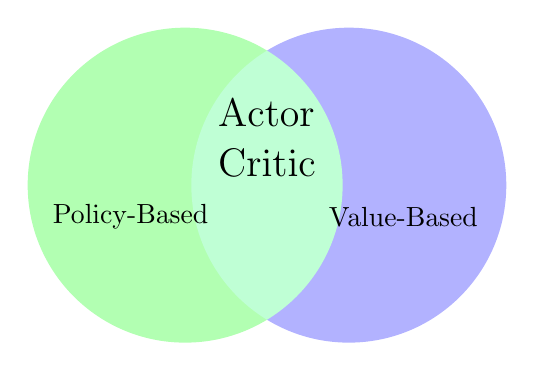
\begin{tikzpicture}
  \begin{scope}[blend group = soft light]
    \fill[green!30!white] (210:1.2) circle (2);
    \fill[blue!30!white]  (330:1.2) circle (2);
  \end{scope}
  \node at ( 210:2)   {Policy-Based};
  \node at ( 330:2)   {Value-Based};
  \node [font=\Large,align=left] {Actor\\ Critic};
\end{tikzpicture}
    \caption{Illustrating the relationship between  Actor-Critic, policy-based and value-based methods}
    \label{fig:actor_critics_venn}
\end{figure}
The most general actor-critic algorithm would look something like this:
\begin{algorithm}[H]
  \large
    \caption{One-Step Actor Critic}\label{general_actor_critic}
    \begin{algorithmic}
        \STATE Init. $s,\theta,w$
        \FOR{$t=0,1,\dots,T$}
        \STATE sample $a_t \sim \pi_{\theta}(s_t)$
        \STATE sample $s_{t+1} \sim P(s_{t+1}|s_t,a_t)$ and  $r_{t+1} \sim R(s_t,a_t)$
        %\STATE $w \gets w + \beta \delta_t\nabla_w V_w(s_t)$
        \STATE Update $V^\pi_w$
        \STATE $A^\pi(s_t,a_t) = r_{t+1} + \gamma V^\pi_{w}(s_{t+1})- V^\pi_{w}(s_t)$
        \STATE $\nabla_\theta J(\theta) \approx \nabla_\theta \log{\pi(a_t|s_t)A^\pi(s_t,a_t)}$
        \STATE $\theta \gets \theta + \alpha \nabla_\theta J(\theta) $
        \ENDFOR
    \end{algorithmic}
\end{algorithm}
There are multiple variants of the actor-critics method which will be looking at in the following.

\section{Off Policy Actor Critic}
The first actor-critic algorithm we examined, presented in Algorithm \ref{general_actor_critic},
is a fully on-policy method. This approach has significant drawbacks, as we discussed in the policy
gradient chapter. Training samples are collected based on the current policy-the very policy we aim
to optimize. As a result, after each gradient update, we can no longer use the previously collected
samples. If the method were off-policy, we could achieve better sample efficiency and enhanced
exploration by following a variety of different policies. This concept will be further explored in the 
following section.
\subsection{First Attempt}
The first idea that comes to mind for making the algorithm off-policy is to introduce a replay buffer,
similar to what we did in the DQN section, resulting in an approach like this:
\begin{algorithm}[H]
  \large
    \caption{}\label{first_off_policy_attempt_act_crit}
    \begin{algorithmic}
        \STATE Init. $s,\theta,w, D = \{\}$
        \FOR{$t=0,1,\dots,T$}
        \STATE sample $a_t \sim \pi_{\theta}(s_t)$
        \STATE sample $s_{t+1} \sim P(s_{t+1}|s_t,a_t)$ and  $r_{t+1} \sim R(s_t,a_t)$
        \STATE store $(s_t,a_t,s_{t+1},r_{t+1})$ in $D$
        \STATE sample a batch $((s_i,a_i,s_{i+1},r_{i+1}))$ from buffer $D$
        \STATE execute Actor Critic Algorithm \ref{general_actor_critic} on batch
        \ENDFOR
    \end{algorithmic}
\end{algorithm}
However, the algorithm has some significant flaws and cannot be used as it is currently written. There are two 
main issues. 
\paragraph{Value Function} The first concerns the target values
$$y_i = r_{i+1} + \gamma V^\pi_{w}(s_{i+1})$$
These targets are incorrect because the batch samples come from older actors, yet we use them to compute target values for 
training the current critic. As a result, the current actor is being guided by targets that reflect outdated policies, rather 
than its own behaviour.\newline 
To address this issue, we will learn the Q-value function instead of the V-function.  Recall that the Q-function represents 
the expected return starting from a given state, taking a specific action, and then following the policy thereafter. Using the 
relationship between the value function and the Q-function given in Equation \eqref{eq:v_to_q}, we can rewrite the target as:
\begin{align*}
    y_i = r_{i+1} + \gamma V^\pi_{w}(s_{i+1}) 
    &=  r_{i+1} + \gamma Q^\pi_{w}(s_{i+1},a') \qquad a' \sim \pi_\theta(\cdot|s_i)
\end{align*}
This allows us to reuse  $s_{t+1}$ from the replay buffer, while sampling the corresponding action $a'$ from the current 
policy. In doing so, our target values remain aligned with the actor's present behaviour. If we had insisted on using the 
value function in an off-policy setting, we would have needed to invoke the simulator to generate the actions the actor would 
take and observe the resulting next states—an expensive and impractical process. In contrast, with this Q-function approach, 
we only need to sample $a'$ from the current policy, which is straightforward since the policy is represented by a neural 
network. Thus, the procedure remains both accurate and efficient.

\paragraph{Policy Gradient} The second problem is that the policy gradient is defined as an expectation over the current 
policy, as seen in Equation \ref{polygrad_td}. This implies that we cannot directly use the samples from the batch. 
We’ve previously discussed how to mitigate this using importance sampling, but another option is to simply
sample again from the current actor, resulting in:
$$\nabla_\theta J(\theta) \approx \nabla_\theta \log{\pi(a_i^\pi|s_i)A^\pi(s_i,a_i^\pi)} \qquad a_i^\pi \sim \pi_\theta(\cdot|s_i) (\text{current actor})$$
%This approach remains efficient, as sampling is quick.\newline\newline 
While some parts of what we have looked at here may seem a bit incoherent/random, I believe this explanation helps to 
understand state of the art off-policy actor-critic methods. These methods are quite similar to what we've discussed here,
so by the time we look at them next, it should feel more familiar when reading the code for these algorithms. 
That’s the goal, at least! As a reminder, policy gradients don't have to be defined solely through the 
advantage function; they can also be defined directly using the Q-function removing the need to also learn a V-function.


%Off-Policy Actor-critics methods have the following structure:
%\begin{enumerate}
%    \item Update critic $Q_\phi(s,a)$ for current policy (arbitrary stochastic behaviour policy not the optimal policy) using off-policy data
%    \item update the actor $\pi_\theta(a|s)$ \begin{itemize}
%        \item stochastic updates: Traditional methods
%        \item deterministic updates: DDPG,TD3
%        \item variational update: SAC
%    \end{itemize}
%\end{enumerate}

\subsection{Updating the critic}
There are multiple ways to update the critic (see Section \ref{section:td-methods} for details) but in most cases, the update 
resembles the approach used in DQN.\newline 
In contrast, there are several different strategies for updating the actor, which we will explore next.

%\subsection{Updating the actor}

%\subsubsection{Stochastic  updates}
%Stochastic updates are among the simplest methods. In this approach, the 
%objective and its gradient are given by:
%$$  J(\theta) = \mathbb{E}_{(s,a)\sim \pi_\theta(a|s)}[A^\pi(s,a)] 
%=  \mathbb{E}_{(s,a)\sim \pi_\theta(a|s)}[Q^\pi(s,a)-V^\pi(s)]$$
%The gradient of the objective is:
%$$ \nabla_\theta J(\theta) =  \mathbb{E}_{(s,a)\sim \pi_\theta(a|s)}
%[\nabla_\theta\log{\pi_\theta(a|s)}\left(Q^\pi(s,a)-V^\pi
%(s)\right)]$$
%The idea here is that we only learn the Value-Function $V$ since we can express the 
%$Q$-Function in terms of it.
%However, this method faces challenges, such as the potential for 
%exploration to collapse too quickly. Additionally, it requires an 
%accurate value function, making the approach more complex.

\subsection{Deterministic updates}
In methods described above, the policy is always modelled as a stochastic policy $\pi(a|s)$. 
Deterministic policy gradient (DPG) instead models the policy as a deterministic decision $a = \pi(s)$.
With this policy the objective of the actor is given by 
$$\max\limits_\theta \underset{s\sim \mathcal{D}}{\mathbb{E}}[Q_\phi(s,\pi_\theta(s))]$$
The gradient of this with respect to $\theta$ is given by
\begin{align*}
\nabla_\theta  \underset{s\sim \mathcal{D}}{\mathbb{E}}[Q_\phi(s,\pi_\theta(s))]
&=  \underset{s\sim \mathcal{D}}{\mathbb{E}}[\nabla_\theta Q_\phi(s,\pi_\theta(s))] \\
&=  \underset{s\sim \mathcal{D}}{\mathbb{E}}\left[ \nabla_a Q_\phi(s,a) \nabla_\theta \pi_\theta(s)|_{a=\pi_\theta(s)}\right]
\end{align*}
At first glance, this may not seem like the policy gradient we derived in the policy gradient chapter. 
However, the deterministic policy gradient is actually a special case of the stochastic policy gradient. 
The proof can be found in \cite{10.5555/3044805.3044850}(Section 3.3).

\subsubsection{Deep Deterministic Policy Gradient (DDPG)} 
DDPG \cite{lillicrap2019continuouscontroldeepreinforcement} is essentially a combination of the deterministic policy
gradient method and DQN, with DQN being used to train the critic. It makes use of the replay buffer and employs the technique 
of using an additional target network for more stable training. The calculation of the max in the target values is addressed 
by using a policy network to compute an action that approximately maximizes the Q-function. Since the policy is deterministic, 
exploration is limited. To encourage better exploration, noise is added to the deterministic policy. 
(see algorithm \ref{algo:ddpg})\newline 
But unfortunately DDPG is quite unstable and requires carefully chosen hyper-parameters. 
Some solutions to this are given with the SAC and TD3 algorithms which we will be looking at in the following.

\subsubsection{Twin Delayed Deep Deterministic (TD3)}
One of the problems with DDPG is that it suffers from overestimation in the learned 
Q-Function. This then leads to the policy breaking, because it exploits the errors 
in the Q-function. Twin Delayed DDPG (TD3) \cite{fujimoto2018addressingfunctionapproximationerror}
is an algorithm (see \ref{algo:TD3}) that addresses this issue by introducing three changes to the original DDPG algorithm.
 \begin{enumerate}
    \item \textbf{Double-Q Learning:} learns two Q-functions instead of one (hence “twin”), and uses
    the smaller of the two Q-values to form the targets in the Bellman error loss functions. 
    Meaning we have critics $(Q_{\phi_1},Q_{\phi_2})$
    \item \textbf{Delayed Policy Updates:} update the policy (and target networks) less frequently than the Q-function.
    \item \textbf{Target Policy Smoothing:} add noise to the target action, to make it harder for the policy to exploit
    Q-function errors by smoothing out Q along changes in action.
 \end{enumerate}

\begin{algorithm}[H]
  \caption{DDPG algorithm from \cite{lillicrap2019continuouscontroldeepreinforcement}\label{algo:ddpg}}
  \begin{algorithmic}
    \STATE Randomly initialize critic network $Q(s, a | \theta^Q)$ and actor
    $\mu(s | \theta^{\mu})$ with weights $\theta^{Q}$ and $\theta^{\mu}$.
    \STATE Initialize target network $Q'$ and $\mu'$ with weights $\theta^{Q'}
    \leftarrow \theta^{Q}$, $\theta^{\mu'} \leftarrow \theta^{\mu}$
    \STATE Initialize replay buffer $R$
    \FOR{episode = 1, M}
      \STATE Initialize a random process $\mathcal{N}$ for action
      exploration
      \STATE Receive initial observation state $s_1$
      \FOR{t = 1, T}
        \STATE Select action $a_t = \mu(s_t | \theta^{\mu}) + \mathcal{N}_t$
        according to the current policy and exploration noise
        \STATE Execute action $a_t$ and observe
        reward $r_t$ and observe new state $s_{t+1}$
        \STATE Store transition $(s_t, a_t,
                r_t, s_{t+1})$ in $R$
        \STATE Sample a random minibatch of $N$ transitions
               $(s_i, a_i,
        r_i, s_{i + 1})$ from $R$
        \STATE Set $ y_i = r_i + \gamma Q'(s_{i + 1},
        \mu'(s_{i+1} | \theta^{\mu'}) | \theta^{Q'}) $
            %\begin{cases}
            %r_t + \gamma Q'(\mathbf{s}_{j + 1}, \mu'(\mathbf{s}_{j+1})) &
            %                      \text {for non terminal } \\
            %                      r_t & \text{ for terminal } \\
            %\end{cases} $
        \STATE Update critic by minimizing the loss:
               $L = \frac{1}{N} \sum_i (y_i -
               Q(s_i, a_i | \theta^Q))^2$
        \STATE Update the actor policy using the sampled policy gradient:
        \begin{equation*}
            \nabla_{\theta^{\mu}} J \approx
            \frac{1}{N} \sum_i
               \nabla_{a} Q(s, a | \theta^Q)|_{s = s_i, a = \mu(s_i)}
               \nabla_{\theta^\mu} \mu(s | \theta^\mu)|_{s_i}
         \end{equation*}
        \STATE Update the target networks:
          \begin{equation*}
            \theta^{Q'} \leftarrow \tau \theta^{Q} + (1 - \tau) \theta^{Q'}
          \end{equation*}
          \begin{equation*}
            \theta^{\mu'} \leftarrow \tau \theta^{\mu} +
                (1 - \tau) \theta^{\mu'}
          \end{equation*}
        \ENDFOR
    \ENDFOR
  \end{algorithmic}
\end{algorithm}


\begin{algorithm}[H]
   \caption{TD3 algorithm from \cite{fujimoto2018addressingfunctionapproximationerror}}
   \label{algo:TD3}
\begin{algorithmic}
   \STATE \setulcolor{red}\ul{Initialize critic networks $Q_{\theta_1}$, $Q_{\theta_2}$, and actor network $\pi_\phi$} 
   with random parameters $\theta_1$, $\theta_2$, $\phi$
   \STATE \setulcolor{red}\ul{Initialize target networks $\theta'_1 \leftarrow \theta_1$, $\theta'_2 \leftarrow 
   \theta_2$, $\phi' \leftarrow \phi$}
   \STATE Initialize replay buffer $\B$
   \FOR{$t=1$ {\bfseries to} $T$}
   \STATE Select action with exploration noise $a \sim \pi_\phi(s) + \e$, 
   \STATE $\e \sim \N(0, \sigma)$ and observe reward $r$ and new state $s'$
   \STATE Store transition tuple $(s, a, r, s')$ in $\B$ 
   \STATE 
   \STATE Sample mini-batch of $N$ transitions $(s, a, r, s')$ from $\B$
   %\STATE Select action with target policy noise: 
   \STATE $\tilde a \leftarrow \pi_{\phi'}(s') + \e, \quad \e \sim \clip(\N(0, \tilde \s), -c, c)$  
   \COMMENT{\textcolor{red}{Target policy smoothing}}
   %\STATE Use Clipped Double Q-learning target:
   \STATE $y \leftarrow r + \y \min_{i=1,2} Q_{\theta'_i}(s', \tilde a)$  \COMMENT{\textcolor{red}{Clipped Double Q-Learning}}
   %\STATE Update $\theta_i$ to minimize $N^{-1} \sum (y - Q_{\theta_i}(s,a))^2$
   %$\{Q_{\theta_i}\}_{i=1}^2$
   \STATE Update critics $\theta_i \leftarrow \argmin_{\theta_i} N^{-1} \sum (y - Q_{\theta_i}(s,a))^2$
    \IF{$t$ mod $d$ \COMMENT{\textcolor{red}{Delayed update}}\newline}
   \STATE Update $\phi$ by the deterministic policy gradient: 
   \STATE $\nabla_{\phi} J(\phi) = N^{-1} \sum \nabla_{a} Q_{\theta_1}(s, a) |_{a=\pi_{\phi}(s)} \nabla_{\phi} \pi_\phi(s)$
   \STATE Update target networks:
   \STATE $\theta'_i \leftarrow \tau \theta_i + (1 - \tau) \theta'_i$
   \STATE $\phi' \leftarrow \tau \phi + (1 - \tau) \phi'$
   \ENDIF
   \ENDFOR
\end{algorithmic}
\end{algorithm}
The comments and underlines added in the following algorithm are not part of the original paper.
They have been included solely to highlight the areas where the new changes have been made, inspired by \cite{Lil'Log_PG}.

\subsection{Variational Actor Updates (Soft Actor Critic (SAC))}\label{SAC}
A problem with the deterministic policy approaches is that they might not explore enough leading to sub optimal policies.
SAC \cite{haarnoja2018softactorcriticoffpolicymaximum} tries to balance exploration and exploitation by using max-entropy reinforcement learning.
It is an algorithm that optimizes a stochastic policy in an off-policy way, forming a bridge between stochastic 
policy optimization and DDPG-style approaches.

\subsubsection{Max-Entropy Reinforcement Learning}
To remind ourself, the entropy  of a random variable $X$ roughly speaking says how random $X$ is and is defined as 
$$ H(X) = \underset{x\sim X}{\mathbb{E}}[-\log{p(x)}]$$ 
In the context of entropy-regularised reinforcement learning, the agent is provided with not only the usual reward, 
but also an entropy term, which changes the problem of finding the optimal policy to:
$$ \pi^* = \argmax\limits_\pi \underset{\tau\sim \pi}{\mathbb{E}}\left[\underset{t=0}{\sum^\infty}\gamma^t(r_t+\alpha H(\pi|s_t)) \right]$$ 
Here $\alpha$ is the \textbf{trade-off coefficient} and controls if the focus should be on maximizing reward or keeping entropy, i.e.
a high $\alpha$ lets the agent focus more on exploration while a small $\alpha$ leads to more exploitation. In the course of this, we can 
also define the corresponding Value/Action-Value-Function 
\begin{equation*}
      V_\text{soft}^\pi(s) =  \underset{\tau\sim \pi}{\mathbb{E}}\left[\underset{t=0}{\sum^\infty}
     \gamma^t(r_t+\alpha H(\pi|s_t))  \giventhat s_0 = s \right] 
\end{equation*}
\begin{align*}
            Q_\text{soft}^\pi(s,a) &=  \underset{\tau\sim \pi}{\mathbb{E}}\left[\underset{t=0}
        {\sum^\infty}\gamma^t r_t + \alpha \underset{\color{red}t=1}{\sum^\infty} 
        \gamma^t H(\pi|s_t) \giventhat s_0=s,a_0=a\right] \\
         &=\underset{\substack{s'\sim P \\ a' \sim \pi}}{\mathbb{E}}[R(s,a)+\gamma \left(Q_\text{soft}^\pi(s',a')+\alpha H(\pi(\cdot,s'))\right)]
\end{align*}
We can then define the functions in terms of each other: \newline
\noindent\begin{minipage}{0.5\linewidth}
    \begin{align}
     V_\text{soft}^\pi(s) &=  \underset{a\sim \pi}{\mathbb{E}}[Q_\text{soft}^{\pi}(s,a)] + \alpha H\left(\pi(\cdot|s)\right)  \label{soft_v_bellman}
    \end{align}
\end{minipage}%
\begin{minipage}{0.5\linewidth}
    \begin{align}
        Q_\text{soft}^\pi(s,a) &=  \underset{s'\sim P}{\mathbb{E}}[R(s,a)+\gamma V_\text{soft}^\pi(s')] \label{soft_q_bellman}
    \end{align}
\end{minipage}\newline\newline 
This V- and Q-Functions are also called the soft V- and soft Q-Function since the entropy regularization prevents
that the policy becomes a ''hard`` maximum operator and always incorporate some exploration.

\subsubsection{Actor and Critic}
SAC sets up the MSBE loss for the critic similar to TD3 by using the clipped double-Q trick with additional target networks,
and taking the minimum Q-value between the two Q approximators. Putting it all together, the loss functions for the Q-networks 
in SAC are:
\begin{gather*}
L(\phi_i, {\mathcal D}) = \underset{(s,a,r,s') \sim {\mathcal D}}{{\mathrm E}}\left[
    \Bigg( Q_{\phi_i}(s,a) - y(r,s') \Bigg)^2
    \right], \text{with} \\
y(r, s') = r + \gamma \left( \min_{j=1,2} Q_{\phi_{\text{targ},j}}(s', \tilde{a}') - \alpha \log \pi_{\theta}(\tilde{a}'|s') \right), \qquad \tilde{a}' \sim \pi_{\theta}(\cdot|s').
\end{gather*}
In order to learn the policy the actor tries to maximize \eqref{soft_v_bellman} which results into
$$ V^\pi(s)= \underset{a\sim \pi_\theta}{\mathbb{E}}[{ \min_{j=1,2} Q_{\phi_j}(s,a) - \alpha \log \pi_\theta(a|s)}]$$ 
In order to take the derivative with respect to $\theta$, one could use the likelihood ratio gradient, as we have seen 
in the policy gradient chapter. However, this approach does not leverage the gradient information from the critic.
Although the action fed into the network is sampled from the policy $\pi_\theta$, the sampling process itself is non-differentiable, 
preventing the direct application of the chain rule to propagate the gradients. To solve this we are going to use the reparametrization 
trick. 

\subsubsection{Reparametrization Trick}\label{reparametrization_trick}
Consider an objective of the form:
$$\argmin\limits_\theta \mathbb{E}_{p_\theta}[f(x)] = \int p_\theta(x) f(x) \, \mathrm{d}x$$
In the context of a computational graph, the challenge arises from the fact that $x \sim p_\theta $
is a random/stochastic node, through which backpropagation cannot be performed.\newline
The idea is to introduce a random variable $\xi \sim q(\xi)$ and a deterministic, differentiable function $g_\theta(\xi)$ 
such that $x = g_\theta(\xi)$, while still having $x \sim p_\theta(x)$. This allows us to rewrite the original expectation as:
$$\mathbb{E}_{x \sim p_\theta}[f(x)] = \mathbb{E}_{\xi \sim q}[f(g_\theta(\xi))]$$
The advantage of this formulation is that when we take the derivative, we are left with an expectation that can 
now be Monte Carlo sampled. Specifically, we have:
\begin{align*}
\nabla_\theta \mathbb{E}_{\xi \sim q}[f(g_\theta(\xi))] &= \nabla_\theta \int q(\xi) f(g_\theta(\xi)) \, \mathrm{d}\xi \\
&= \int q(\xi) \nabla_\theta f(g_\theta(\xi)) \, \mathrm{d}\xi \\
&= \int q(\xi) \frac{\mathrm{d} f}{\mathrm{d} g_\theta(\xi)}(g_\theta(\xi)) \frac{\mathrm{d} g_\theta}{\mathrm{d} \theta}(\xi) 
\, \mathrm{d}\xi \\
&= \mathbb{E}_{\xi \sim q}\left[ \frac{\mathrm{d} f}{\mathrm{d} g_\theta(\xi)}(g_\theta(\xi)) \frac{\mathrm{d} g_\theta}{\mathrm{d} \theta}
(\xi)\right]
\end{align*}
In SAC for continuous action spaces, the policy is Gaussian distributed, i.e., $\pi_\theta(a|s) \sim \mathcal{N}(\mu, \Sigma)$. Here, the 
choice of $q(\xi)$ and $g_\theta(\xi)$ is given by:
$$g_\theta(\xi) = \mu + A\xi \quad \text{s.t.} \quad A^T A = \Sigma$$
After applying the reparameterization trick, we are left with the following objective for the actor
$$\max_{\theta} \underset{\substack{s \sim \mathcal{D} \\ \xi \sim \mathcal{N}}}{\mathbb{E}}\left[{\min_{j=1,2} Q_{\phi_j}
(s,\tilde{a}_{\theta}(s,\xi)) - \alpha \log \pi_{\theta}(\tilde{a}_{\theta}(s,\xi)|s)}\right]$$
Unlike in TD3, which uses $Q_{\phi_1}$ (just the first Q approximator), SAC uses $\min_{j=1,2} Q_{\phi_j}$ (the minimum of the two Q approximators).
\begin{figure}[H]
\begin{minipage}[t]{0.48\textwidth}
\centering
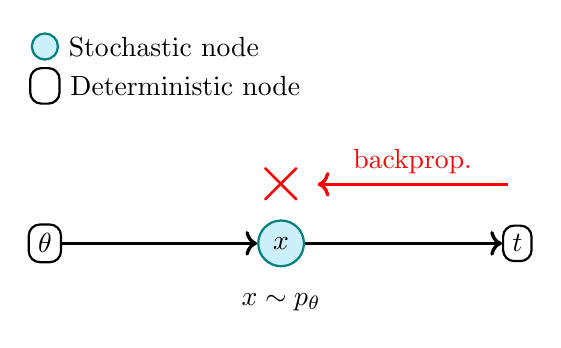
\begin{tikzpicture}
\node[rectangle, rounded corners, thick, draw] (A) at (0,0) {$\theta$};
\node[circle, fill=cyan!20!white, draw=teal, text=black, thick] (B) at (3,0) {$x$};
\node[fill=none]  at (3, -0.75) {$x\sim p_\theta$};

\node[circle, fill=cyan!20!white, draw=teal, text=black, thick] (stoch) at (0,2.5) {};
\node[anchor=west] at (stoch.east) {Stochastic node};
\node[rectangle, rounded corners, thick, draw] (det) at (0,2) {\color{white} t};
\node[anchor=west] at (det.east) {Deterministic node};

\node[rectangle, rounded corners, thick, draw] (C) at (6,0) {$t$};
\node[fill=none, text=red,font=\Huge] (X) at (3, 0.75) {$\times$};
\node[fill=none, text=red] (E) at (6, 0.75) {};

\path[->, very thick] (A) edge node {} (B);
\path[->, very thick] (B) edge node {} (C);
\path[->, red, very thick] (E) edge node[above] {backprop.} (X);
\end{tikzpicture}
\end{minipage}%
\hfill
\begin{minipage}[t]{0.48\textwidth}
\centering
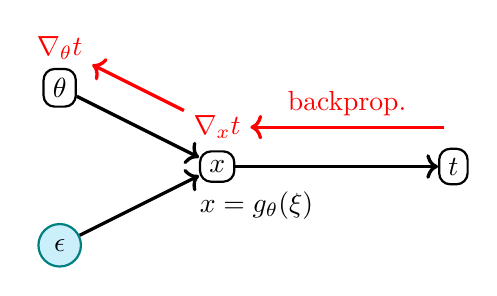
\begin{tikzpicture}
\node[rectangle, rounded corners, thick, draw] (A) at (0,0) {$\theta$};
\node[circle, fill=cyan!20!white, draw=teal, text=black, thick] (Eps) at (0,-2) {$\epsilon$};
\node[rectangle, rounded corners, thick, draw] (B) at (2,-1) {$x$};
\node[fill=none,]  at (2.5,-1.5) {$x=g_\theta(\xi)$};
\node[rectangle, rounded corners, thick, draw] (C) at (5,-1) {$t$};

\node[fill=none, text=red] (X) at (2, -0.5) {$\nabla_x t$};
\node[fill=none, text=red] (E) at (5, -0.5) {};
\node[fill=none, text=red] (S) at (0, 0.5) {$\nabla_\theta t$};

\path[->, very thick] (A) edge node {} (B);
\path[->, very thick] (B) edge node {} (C);
\path[->, very thick] (Eps) edge node {} (B);
\path[->, red, very thick] (E) edge node[above] {backprop.} (X);
\path[->, red, very thick] (X) edge node[above] {} (S);
\end{tikzpicture}
\end{minipage}
\caption{Computational graphs for the objective without the reparameterization trick (left) and with it (right).
By isolating the stochasticity into a separate node, we enable gradient computation with respect to the model parameters.}
\label{fig:repar_trick_visual}
\end{figure}
 Ultimately, we are left with the following SAC algorithm:
 
\begin{algorithm}[H]
\caption{Soft Actor-Critic from \cite{haarnoja2018softactorcriticoffpolicymaximum} (original)}
\label{alg:soft_actor_critic}
\begin{algorithmic}
\STATE \mbox{Initialize parameter vectors $\psi, \bar{\psi}, \theta, \phi$.}
\FOR{each iteration}
	\FOR{each environment step}
	\STATE $a_t \sim \pi_\phi(a_t|s_t)$
	\STATE $s_tp \sim p(s_tp| s_t, a_t)$
	\STATE $\mathcal{D} \leftarrow \mathcal{D} \cup \left\{(s_t, a_t, r(s_t, a_t), s_{t+1})\right\}$
	\ENDFOR
	\FOR{each gradient step}
	\item $\psi \leftarrow \psi - \lambda_V \hat \nabla_\psi J_V(\psi)$
	\STATE $\theta_i \leftarrow \theta_i - \lambda_Q \hat \nabla_{\theta_i} J_Q(\theta_i)$ for $i\in\{1, 2\}$
	\STATE $\phi \leftarrow \phi - \lambda_\phi \hat \nabla_\phi J_\phi(\phi)$
	\STATE $\bar{\psi}\leftarrow \tau \psi + (1-\tau)\bar{\psi}$
	\ENDFOR
\ENDFOR
\end{algorithmic}
\end{algorithm}

\begin{algorithm}[H] 
\caption{Soft Actor-Critic (OpenAI's Spinning Up version \cite{OpenAI_Spinning_UP})} 
\label{alg:SAC} 
\begin{algorithmic} 
\STATE Input: initial policy parameters $\theta$, Q-function parameters $\phi_1$, $\phi_2$, empty replay buffer $\mathcal{D}$ 
\STATE Set target parameters equal to main parameters $\phi_{\text{targ},1} \leftarrow \phi_1$, $\phi_{\text{targ},2} \leftarrow \phi_2$ 
\REPEAT \STATE Observe state $s$ and select action $a \sim \pi_{\theta}(\cdot|s)$ 
\STATE Execute $a$ in the environment 
\STATE Observe next state $s'$, reward $r$, and done signal $d$ to indicate whether $s'$ is terminal 
\STATE Store $(s,a,r,s',d)$ in replay buffer $\mathcal{D}$ 
\STATE If $s'$ is terminal, reset environment state. 
\IF{it's time to update} 
\FOR{$j$ in range(however many updates)} 
\STATE Randomly sample a batch of transitions, $B = \{ (s,a,r,s',d) \}$ from $\mathcal{D}$ 
\STATE Compute targets for the Q functions: \begin{align*} y (r,s',d) &= r + \gamma (1-d) \left(\min_{i=1,2} Q_{\phi_{\text{targ}, i}} (s',
\tilde{a}') - \alpha \log \pi_{\theta}(\tilde{a}'|s')\right), && \tilde{a}' \sim \pi_{\theta}(\cdot|s') \end{align*} 
\STATE Update Q-functions by one step of gradient descent using \begin{align*} & \nabla_{\phi_i} \frac{1}{|B|}\sum_{(s,a,r,s',d) \in B} 
\left( Q_{\phi_i}(s,a) - y(r,s',d) \right)^2 && \text{for } i=1,2 \end{align*} 
\STATE Update policy by one step of gradient ascent using \begin{equation*} \nabla_{\theta} \frac{1}{|B|}\sum_{s \in B} \Big(\min_{i=1,2} 
Q_{\phi_i}(s, \tilde{a}_{\theta}(s)) - \alpha \log \pi_{\theta} \left(\left. \tilde{a}_{\theta}(s) \right| s\right) \Big), \end{equation*} 
where $\tilde{a}_{\theta}(s)$ is a sample from $\pi_{\theta}(\cdot|s)$ which is differentiable wrt $\theta$ via the reparametrization trick. 
\STATE Update target networks with \begin{align*} \phi_{\text{targ},i} &\leftarrow \rho \phi_{\text{targ}, i} + (1-\rho) \phi_i && \text{for } i=1,2 \end{align*} 
\ENDFOR 
\ENDIF 
\UNTIL{convergence} 
\end{algorithmic} 
\end{algorithm}


\subsection{CrossQ}
CrossQ \cite{bhatt2024crossqbatchnormalizationdeep} attempts to introduce batch 
normalization into Q-learning. But what exactly is batch normalization?\newline
Batch normalization is a technique used in deep learning to improve the training of neural 
networks by normalizing the inputs to each layer. It works by adjusting and scaling the 
activations (outputs of neurons). Specifically, it standardizes these activations by 
subtracting the batch mean and dividing by the batch standard deviation, followed by 
scaling and shifting using learnable parameters. Batch normalisation has many benefits such 
as:
\begin{itemize}
    \item Faster Training: It helps the network converge faster by reducing internal 
    covariate shift (i.e., the changing distribution of inputs to each layer during 
    training), making the process more stable.
    
    \item Improved Performance: It often leads to better generalization, reducing 
    overfitting, and improving model performance on unseen data.
    
    \item Allows Higher Learning Rates: Batch normalization enables the use of higher 
    learning rates without causing instability in the training process.
\end{itemize}
However, several people have found that standard batch normalization doesn't work well with 
Q-learning and often makes the learning process more unstable. The issue lies in how the 
Temporal Difference (TD) error is computed in reinforcement learning. So in general the 
loss is defined as 
\begin{align*}
    L_\psi &= \left(\max_{a'}Q_{\psi'}(s_{t+1},a') + r_t - Q_\psi(s_t,a_t)\right)^2 \\
     &= \left(Q_{\psi'}(s_{t+1},\mu_\psi(s)) + r_t - Q_\psi(s_t,a_t)\right)^2 
\end{align*}
%$$ L_\psi = \left(Q_{\psi'}(s_{t+1},a') + r_t - Q_\psi(s_t,a_t)\right)^2$$
where $(s_t,a_t,r_t,s_{t+1})$ are samples from the replay buffer. While $s_t$ and $s_{t+1}$
come from the same distribution, $a_t$ is from the replay buffer, and $a'$ is the action 
predicted by the neural network (which corresponds to the argmax action). This means that
$a_t$ and $a'$ are distributed differently. Since batch normalization requires samples to be independent and identically 
distributed (iid), this discrepancy in distributions introduces the problem. The solution to 
this issue is to concatenate the different state and action batches into a single batch, 
ensuring that all inputs come from the same mixture distribution.
\begin{gather*}
     Q_\psi\left(\begin{bmatrix}
    s_t\\s_{t+1}
\end{bmatrix}, 
\begin{bmatrix}
    a_t\\a'
\end{bmatrix}\right) = \begin{bmatrix}
    q_t\\q_{t+1}
\end{bmatrix} \\
L_\psi = \left(\text{StopGradient}(q_{t+1})+r_t-q_t\right)^2
\end{gather*}
This procedure makes training faster and more efficient overall, as it eliminates the need for a target network.

\subsection{BRO}
The BRO (Bigger, Regularized, Optimistic) paper \cite{nauman2024biggerregularizedoptimisticscaling} shows that scaling model capacity—alongside strong regularization and optimistic 
exploration—can significantly boost sample efficiency in reinforcement learning. Unlike traditional approaches that rely mainly on algorithmic tweaks, BRO leverages large critics and task-specific enhancements to achieve state-of-the-art performances. 

\subsection{Self-Test Questions}
\begin{enumerate}
\sq{ What is the role of the critic in actor-critic methods?}\newline
The critic calculates the TD-Error and tries to learn the value/action-value function

\sq{ Which methods do you know for computing the critic?}\newline
Single sample estimates, N-step returns and Generalized advantage estimation

\sq{Why are off-policy methods more efficient then on-policy methods}\newline
The can use previous collected data to do updates and do not always have to generate new data/discard old data. It also promotes exploring if the samples are chosen randomly from the buffer.

\sq{How can we achieve off-policy RL with continuous actions}\newline
Computing the maximum over actions in the target is a challenge in continuous action spaces. Some solutions are \begin{itemize}
    \item finding the max by doing gradient descent on the Q-network
    \item random shooting: randomly select some actions and take the best performing out of them for calculating the target.
    \item iterative stochastic optimization: same as random shooting but we iteratively update the distribution from which we draw samples to get a better action at the end
    \item learning a neural network to predict the max action
\end{itemize}

\sq{What are the different options to optimize the actor?}\begin{itemize}
    \item stochastic: normal policy gradient where the reward is now changed to be the advantage function
    \item deterministic: learn a deterministic policy that approximates the max operator
    \item variational: regularize RL objective with entropy 
\end{itemize}

\sq{Why do we have a bias in actor critic algorithms and how to fix it?}\newline
The problem is that we use approximators to calculate the targets and since they are bias actor-critics are also bias. That approximator will usually be randomly initialized so it will not give a true estimation of the return, it will be biased towards some random value that was initialized with.

\sq{What type of gradient is DDPG using and why can we not apply the same gradient for the sampled return?}\newline DDPG uses $ \nabla_\theta  \underset{s\sim \mathcal{D}}{\mathbb{E}}[Q_\phi(s,\pi_\theta(s))]
=  \underset{s\sim \mathcal{D}}{\mathbb{E}}\left[ \nabla_a Q_\phi(s,a) \nabla_\theta \pi_\theta(s)|_{a=\pi_\theta(s)}\right]
$

\sq{What is the objective of max-ent reinforcement learning and why is that 
useful?}\newline In entropy-regularized reinforcement learning, the agent gets a bonus 
reward at each time step proportional to the entropy of the policy at that time step. The 
new objective is to maximise this reward. The entropy maximization leads to policies that 
can explore more.

\sq{How to we obtain the policy update in SAC?}
We take the derivative of the Value-Function (Q-Value + Entropy) but with the help 
of the reparametrization trick in order to make the gradient flow through the critic.

\sq{What is the reparametrization trick and when should it be preferred to the likelihood policy gradients?}
It is a trick, in which a sample from $\pi_{\theta}(\cdot|s)$ is drawn by computing a deterministic function of state, policy parameters, and independent noise. The reparametrization trick makes it possible to use the knowledge of the gradient of the Q-function approximation to calculate the gradient of the objective.
\end{enumerate}

\subsection{Resources}
A helpful introduction to actor-critic methods, including the off-policy variants, is provided in Sergey Levine’s CS 285: 
Lecture 6 \cite{CS285,CS285LevineYoutube}. Additionally, the blog posts from OpenAI's Spinning Up series on DDPG, TD3, and SAC 
are excellent resources \cite{OpenAI_Spinning_UP}. For CrossQ, the video \cite{CrossQ_Talk} was particularly informative. For 
BRO, the official website \cite{BRO_Website} offers well-written explanations for those seeking more detailed information.

\section{Control as Inference}
This is a brief exploration into the question of what constitutes optimal behaviour. Traditionally, we’ve 
assumed that the behaviour we want to imitate is perfectly optimal. However, this assumption is not realistic
since humans rarely act in strictly optimal ways.\newline
In this section, we explore Control as Inference, a paradigm that reimagines reinforcement learning not as a strict 
reward-maximisation problem, but as an inference problem within a probabilistic framework. This approach allows us to 
model and tolerate sub-optimal behaviour. We begin with an introduction to variational inference which forms the 
foundation for this reformulation

\subsection{Variational Inference}
A central challenge in modern statistics, especially Bayesian statistics, is approximating complex, intractable 
probability distributions, such as posterior densities like 
$$p(z|x) = \frac{p(x|z)p(z)}{p(x)} = \frac{p(x|z)p(z)}{\int_z p(x,z')\, dz'}$$
where $z$ represents the latent variables and $x$ represents the observed data. The marginalization over $z$ to 
calculate $p(x)$ in the denominator is typically intractable, because, for example, the search space of $z$ is too 
large. Traditional methods like Markov Chain Monte Carlo offer accurate sampling but are often computationally 
expensive, particularly for large datasets or complex models. \newline
Variational Inference (VI) provides a faster alternative by reframing inference as an optimization problem. Instead 
of sampling, VI approximates the true posterior by selecting the closest distribution $q_\theta(z)$ (from a simpler, 
predefined family) using a dissimilarity measure such as Kullback-Leibler (KL) divergence in order to find 
the best paramerters $\theta$.\newline 
In the following, we will explore how the most common discrepancy measure, the Kullback-Leibler divergence, can be 
used for inference. Additionally, in the upcoming discussion, $p^*(x)$ will represent the true probability 
distribution, while  $q(x)$ will denote the approximation.

\subsubsection{Minimizing Reverse KL}
Minimizing the reverse KL divergence is often referred to as (I)nformation-projection and is defined as:
$$\text{KL}(q(x)||p^*(x)) = \int_x q(x)\log{\frac{q(x)}{p^*(x)}} \diff x$$
This objective is also known for its zero-forcing behaviour. This term arises from how the reverse KL divergence 
behaves in regions where the true distribution $p^*(x)$ has high probability mass, but the approximate distribution 
$q(x)$ assigns little or no mass. Consider two cases:
\begin{itemize}
    \item If $p^*(x) > 0$ but $q(x) \approx 0$, then the ratio $\frac{q(x)}{p^*(x)}$ inside the logarithm becomes 
    very small. However, since $q(x) \log(\cdot)$ is multiplied by a value close to zero, the overall contribution to 
    the KL divergence is negligible.    
    \item If $q(x) > 0$ and $p^*(x) = 0$, then the ratio becomes infinite, and $\log(\infty) = \infty$. This causes 
    the 
    KL divergence to become infinitely large, leading the optimization to avoid placing mass in such regions.
\end{itemize}
Therefore, minimizing the reverse KL forces $q(x)$ to avoid assigning probability mass where $p^*(x) = 0$. This 
behavior leads to mode-seeking: reverse KL tends to concentrate $q(x)$ on one mode of $p^*(x)$, ignoring regions of 
low probability. And as long as we are able to sample from $q(x)$, we can approximate the KL divergence using Monte 
Carlo integration.

\subsubsection{Minimizing Forward KL}
Minimizing the forward KL divergence is often referred to as (M)oment-projection and is defined as:
$$\text{KL}(p^*(x)||q(x)) = \int_x p^*(x)\log{\frac{p^*(x)}{q(x)}} \diff x$$
This objective exhibits probability forcing: if the true distribution $p^*(x)$ is high in a region, 
then the approximation $q(x)$ must also be high there to avoid a large penalty. So it got the following properties:
\begin{itemize}
    \item It tends to average over multiple modes of $p^*(x)$, even when the approximation family cannot represent 
    such multimodality well.
    \item It requires samples from the true distribution $p^*(x)$, making it generally unsuitable for variational 
    inference 
    $$ \int_x p^*(x)\log{\frac{p^*(x)}{q(x)}} \diff x = \mathbb{E}_{\color{red}x \sim p^*(x)}\left[\frac{p^*(x)}{q(x)}\right]$$
    \item Minimizing the forward KL is equivalent to maximum likelihood estimation (MLE).
    $$ \int_x p^*(x)\log{\frac{p^*(x)}{q(x)}} \diff x = \text{const }- \int_x p^*(x)\log{q(x)} \diff x$$
\end{itemize}

\begin{figure}[H]
    \centering
    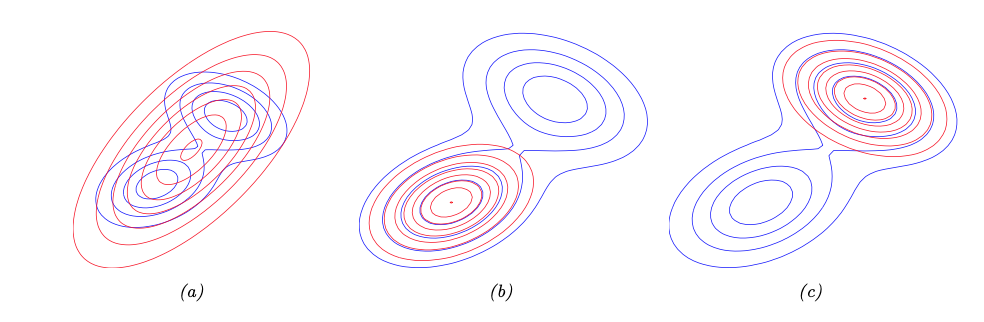
\includegraphics[width=0.9\linewidth]{images/rev_forw_kl.png}
    \caption{Illustrating forward vs. reverse KL. The blue contours represent the true distribution $p^*$, 
    and the red contours are from the approximation $q$. (a) Minimizing forward KL. (b–c) Minimizing reverse KL, 
    where $q$ fits onto different modes each time. }
    \label{fig:reverse_vs_forward_kl}
\end{figure}

\subsection{Connection between Variational Inference and Control}
As mentioned earlier, our current understanding does not allow us to account for suboptimal behaviour in our algorithms. Consider, for 
example, a task where we are required to move a dot on a screen to a goal using a joystick. The optimal behaviour in this scenario would
be to take the straight path, but small deviations may occur due to factors such as lack of concentration or external distractions. Despite
these deviations, we still achieve the same outcome as if we had followed the optimal path. Intuitively, we recognize that small errors do 
not necessarily prevent the task from being successfully completed. Therefore, it is clear that some mistakes are more consequential than 
others when completing a task while still achieving the overall goal.\newline
To incorporate suboptimality into our model, we begin by adding the concept of optimality to the general structure of a MDP. We introduce an 
optimality variable $o_t$, where $o_t = 1$ indicates that time step $t$ is optimal, and $o_t = 0$ indicates that it is not. The corresponding 
graphical model is illustrated as follows
\begin{figure}[H]
    \centering
\resizebox{!}{3.25cm}{
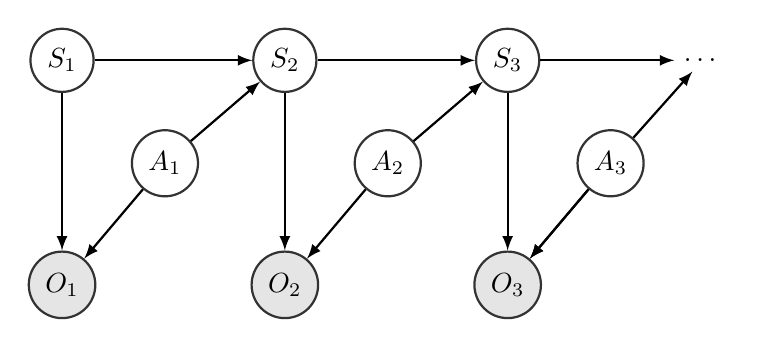
\begin{tikzpicture}
\tikzset{
  main/.style={circle, minimum size = 5mm, thick, draw =black!80, node distance = 20mm},
  connect/.style={-latex, thick},
  box/.style={rectangle, draw=black!100}
}
  \node[main] (L1) [] {$S_1$};
  \node[main] (L2) [right=of L1] {$S_2$};
  \node[main] (L3) [right=of L2] {$S_3$};
 % \node[main] (Lt) [right=40mmof L3] {$S_t$};
  \node[] (Lhid) [right=17mmof L3] {$\dots$};
  
\node[main] (A1) [below right=10mm of L1] {$A_1$};
\node[main] (A2) [below right=10mm of L2] {$A_2$};
\node[main] (A3) [below right=10mm of L3] {$A_3$};
%\node[main] (At) [below left=10mm of Lt] {$A_{t-1}$};


  \node[main,fill=black!10] (O1) [below=of L1] {$O_1$};
  \node[main,fill=black!10] (O2) [below=of L2] {$O_2$};
  \node[main,fill=black!10] (O3) [below=of L3] {$O_3$};
  %\node[main,fill=black!10] (Ot) [below=of Lt] {$O_t$};
  \path (L1) edge [connect] (L2)
        (L2) edge [connect] (L3)
        (L3) edge [connect] (Lhid);
        %(Lhid) edge [connect] (Lt);
        
  \path (A1) edge [connect] (O1)
        (A1) edge [connect] (L2)
        (A2) edge [connect] (O2)
        (A2) edge [connect] (L3)
        (A3) edge [connect] (O3)
        (A3) edge [connect] (O3)
        (A3) edge [connect] (Lhid);
        %(At) edge [connect] (Lt);
  \path (L1) edge [connect] (O1);
  \path (L2) edge [connect] (O2);
  \path (L3) edge [connect] (O3);
  %\path (Lt) edge [connect] (Ot);
\end{tikzpicture}}

\end{figure}
This model resembles a Hidden Markov Model. We now define some probabilities, which may initially appear arbitrary. 
However, they will lead to an elegant framework. For now, we take them as given:
\begin{gather*}
    p(\tau) = p(s_1, a_1, \dots, s_T) = p(s_1) \prod_{t=1}^{T-1} p(s_{t+1} \mid s_t, a_t) \underbrace{\pi(a_t \mid s_t)}_{1\ 
    \text{(uniform)}} \\
    p(o_t \mid s_t, a_t) \propto \exp(r(s_t, a_t)) \\
    p(o_{1:T} \mid \tau) = \exp\left(\sum_{t=1}^T r(s_t, a_t)\right)
\end{gather*}
Our goal is to infer the most likely trajectory given that the agent acts optimally. This means we want to compute 
the posterior:
\begin{equation}
    p(\tau \mid o_{1:T} = 1) = \frac{p(\tau)\,p(o_{1:T} = 1 \mid \tau)}{p(o_{1:T} = 1)} \label{infer_poste}
\end{equation}
Once we have this posterior, we can use marginalization and conditioning to compute the optimal policy:
$$p(a_t \mid s_t, o_{1:T} = 1)$$
The distribution \eqref{infer_poste} can be challenging to compute directly, so we turn to variational inference. 
Specifically, we minimize the reverse KL divergence between an approximate distribution $q_\theta(\tau)$ and the true 
posterior.\newline
We define our variational distribution $q_\theta(\tau)$ as follows (again, this form might seem arbitrary, but it is 
motivated by deeper theory—see resources for details):
$$
q_\theta(\tau) = p(s_1) \prod_t p(s_{t+1} \mid s_t, a_t)\, q_\theta(a_t \mid s_t)
$$
Minimizing the reverse KL divergence gives us the following objective:
\begin{align*}
    \text{KL}(q_\theta(\tau)|| p(\tau|o_\tau=1)) &= \int q_\theta(\tau) \log{ \frac{p(\tau){p(o_\tau=1 | \tau)}}{q_\theta(\tau)\color{green!50!black}p(o_\tau=1)}} \diff \tau \\
    &=\int q_\theta(\tau)\log{p(o_\tau|\tau)}\diff \tau - \text{KL}(q_\theta(\tau)||p(\tau)) + \text{\color{green!50!black}const} \\
    &=\int q_\theta(\tau)\log{p(o_\tau|\tau)}\diff \tau - \int q_\theta(\tau)\log{\frac{q_\theta(\tau)}{p(\tau)}}\diff \tau \\
    &= \int  q_\theta(\tau) \left(\log{p(o_\tau|\tau)} - \log{\frac{q_\theta(\tau)}{p(\tau)}}\right) \diff \tau \\
    &= \int  q_\theta(\tau) \left(\log{p(o_\tau|\tau)} - \log{\frac{ p(s_1)\prod_t p(s_{t+1}|s_t,a_t)q_\theta(a_t|s_t)}{ p(s_1) \prod_{t}p(s_{t+1}|s_t,a_t)}}\right) \diff \tau \\
    &=\int  q_\theta(\tau) \left(\log{p(o_\tau|\tau)} - \log{\prod_t q_\theta(a_t|s_t)}\right) \diff \tau \\
    &=\int  q_\theta(\tau) \left(\log{\left(\exp(\sum_{t=0}^T r(s_t,a_t))\right)} - \log{\prod_t q_\theta(a_t|s_t)}\right) \diff \tau \\
    &=\int  q_\theta(\tau) \left(\sum_t r(s_t,a_t) -\log{q_\theta(a_t|s_t)}\right) \diff \tau \\
    &=  \mathbb{E}_{(s_{1:T},a_{1:T})\sim q_\theta}\left[\sum_t r(s_t,a_t) -\log{q_\theta(a_t|s_t)}\right] \\
    &=  \sum_t\mathbb{E}_{(s_t,a_t)\sim q_\theta}\left[r(s_t,a_t) +H(q_\theta(a_t|s_t))\right] 
\end{align*}
This objective is identical to the one encountered in maximum entropy reinforcement learning, specifically when we 
discussed Soft Actor-Critic (SAC) in Section~\ref{SAC}. In that sense, SAC can be interpreted as performing the 
expected information projection (I-projection).\newline
It’s worth noting that, in this setting, exact inference over the Hidden Markov Model (HMM) could also be performed 
using the forward-backward algorithm. However, we will not cover that here. For those interested, the resources 
provided include further materials that explore this topic in more depth.

\subsection{Resources}
A great introduction to variational inference can be found in \cite{Blei_2017}. Another excellent resource is 
''CS 285: Lecture 18 – Variational Inference`` by Sergey Levine, which provides an intuitive and accessible overview. 
In ''Lecture 19 – Control as Inference``, he derives many of the equations referenced above, which we treated as 
given, and shows how to perform \textbf{exact} inference using the forward-backward algorithm to compute the 
posterior \cite{CS285,CS285LevineYoutube}. Much of the material in these lectures is based on his tutorial 
Reinforcement Learning and Control as Probabilistic Inference 
\cite{levine2018reinforcementlearningcontrolprobabilistic}.
\section{Trust Regions for Policy Gradients }
One problem that arises with policy gradients methods is that the distance in 
parameter space does not translate into policy space. As a result, small changes in 
the parameters can lead to a large changes in policy behaviour. This could even go 
so far as to make our policy so bad that we cannot recover from it. A popular method 
is to limit the difference between subsequent policies to increase stability.

\subsection{Trust regions}
To ensure that the difference between subsequent policies remains limited, we can reformulate the general
objective of maximizing with respect to both the previous and current policies as we did in section \ref{data_reuse}.
This formulation includes an additional constraint to prevent large differences between consecutive policies which 
is achieved by limiting a dissimilarity measure  $D(\cdot,\cdot)$ (i.e. Kullback-Leibler divergence) between the distributions:
\begin{gather*}
\theta_{\text{new}} = \argmax\limits_\theta \mathbb{E}_{(s,a)\sim \pi_{\text{old}}}\left[\frac{\pi_{\theta}(a|s)}{\pi_{\text{old}}(a|s)} A^{\pi_{\text{old}}}(s,a)\right] \qquad  
\text{s.t. } D(\pi_\theta(a|s),\pi_{\text{old}}(a|s)) \leq \epsilon, \forall s \in S
\end{gather*}
We now have a constrained optimization problem that requires specialized methods for solving, which we will look at next.

\subsection{Lagrangian Multipliers}\label{lagrangian_multipliers}
We start by introducing the following optimisation problem:
$$ \underbrace{\min\limits_x f(x)}_{\text{objective}} \qquad \text{s.t } 
\underbrace{h_i(x) \geq b_i, \text{ for } i=1\dots K}_{\text{constraints}}$$
We then define the Lagrangian function/ Lagrangian , which combines the objective and constraint into a single function:
$$ L(x,\lambda) = f(x)- \underset{i=1}{\sum^K}\lambda_i(h_i(x)-b_i) \quad \text{s.t. } \lambda_i \geq 0, \text{ for } i= 1\dots K$$
We call the $\lambda_i$ the Lagrange multipliers. There are now two ways how we can solve this problem in order to solve our original 
optimization problem :
\vspace{-1.2cm}
\begin{multicols}{2}
   \begin{gather*}
      \textbf{Primal optimization problem} \\
      \min\limits_x \max\limits_\lambda L(x,\lambda) 
  \end{gather*}\break
  \begin{gather*}
      \textbf{Dual optimization problem} \\
      \lambda^* = \argmax\limits_\lambda g(\lambda), \qquad g(\lambda)=\min\limits_x L(x,\lambda)
  \end{gather*}
\end{multicols}
The question now is: which problem should we choose to solve, and do we actually obtain the optimal solutions through 
this approach?\newline
The solutions of the primal problem also minimize the unconstrained objective. However, solving the primal problem can
often be challenging, especially since it might not possess the necessary convexity properties, making it hard to solve
directly. But what about the dual function?\newline
Since $ g(\lambda) $ is a pointwise minimum of affine functions (note that $ \mathcal{L}(x, \lambda) $ is affine in $ \lambda $,
even though $ f(x) $ might not be linear or affine but we treat it as a constant with respect to $ \lambda $), the dual function 
is concave (see the proof \cite{Proof_Lagrangian_Concave}). Since $ g(\lambda) $ is concave 
and the constraints are linear (meaning they are convex), maximizing $ g(\lambda) $ over $ \lambda $ is a convex optimization problem. 
Furthermore, because convex functions have the property that every local minimum is also a global minimum, it is easier to solve using 
standard optimization techniques than the primal problem.\newline
But what can we say about the solutions from both methods? Any feasible solution to the primal problem is at least as large 
as any feasible solution to the dual problem. Therefore, the solution to the primal provides an upper bound to the solution 
of the dual, and the solution of the dual provides a lower bound to the solution of the primal. This fact is known as 
\textbf{weak duality}:
$$
g(\lambda) = \min_{x} \mathcal{L}(x, \lambda) \leq \min_{x} f(x) = p^* \quad \Rightarrow \quad d^* = \max_{\lambda} g(\lambda) \leq p^*
$$
In general the optimal values of the primal and dual problems, $ p^* $ and $ d^* $ do not need be equal. The difference between them 
is called the \textbf{duality gap}.
\subsubsection{Lagrangian Multipliers cookbook}
\begin{enumerate}
    \item Write down Langrangian  $L(x,\lambda) = f(x)- {\sum_{i=1}^K}\lambda_i(h_i(x)-b_i)$
    \item Obtain optimal solution for primal parameters (primal solution) $\frac{\text{d}L(x,\lambda)}{\text{d}x} = 0 
    \rightarrow x^* = u(\lambda)$
    \item put $x^*$ back into the Lagrangian $g(\lambda) = L(u(\lambda),\lambda)$
    \item obtain optimal solution for $g(\lambda) \rightarrow \lambda^* = \argmax\limits_\lambda g(\lambda), 
    \text{ s.t. } \lambda_i \geq 0 \;\forall i$
    \item $x^* = u(\lambda^*)$
\end{enumerate}
An important aspect of using the Lagrangian is how to construct it, depending on the type of optimization problem and constraints.
Consider the following simple example:
\begin{gather*}
    \min\limits_x x^2 \text{ s.t. } x\geq1 \longrightarrow L(x,\lambda)= x^2 - \lambda(x-1)
\end{gather*}
The Lagrangian must be constructed in such a way that violating the constraint will not lead to an optimal solution.
Since Lagrange multipliers are non-negative (i.e., $\lambda \geq 0$), violating the constraint $x \geq 1$ would result in adding a positive 
term, even though the goal is to minimize the objective function. This ensures that when $x < 1$ the Lagrangian penalizes this violation,
and vice versa for a maximization problem. To gain a deeper understanding, let’s now consider a more complex example.
\begin{gather*}
  \underset{\boldsymbol{\omega}}{\textrm{argmax}} \int p_{\boldsymbol{\omega}}(\boldsymbol{\theta})g(\boldsymbol{\theta}) 
  d\boldsymbol{\theta} \quad \textrm{s.t.} \quad \textrm{KL}(p_{\boldsymbol{\omega}}(\boldsymbol{\theta}) || p_{\textrm{old}}
  (\boldsymbol{\theta})) \leq \epsilon, \quad \textrm{H}(p_{\boldsymbol{\omega}}(\boldsymbol{\theta})) \geq \beta, \quad \int 
  p_{\boldsymbol{\omega}}(\boldsymbol{\theta}) d \boldsymbol{\theta}=1.
\\
\rightarrow L(p_w,\eta,\kappa) = \int p_w(\theta)g(\theta)d\theta + \eta \left(\epsilon - \textrm{KL}(p_w(\theta)||p_{\textrm{old}}(\theta))\;\right)+\kappa (\textrm{H}(p_w(\theta))-\beta) + \lambda \left( \int p_w(\theta)d\theta -1\right)
\end{gather*}
Notice how we now use $+$ instead of $-$ because this is a maximization problem. And try verifying for yourself, for each of the constraints,
what the outcome (in terms of sign) would be if they were violated. Does this help or penalize in finding the optimal solution?

 \subsection{Trust Region Policy Optimization (TRPO)}
 One of the first methods to introduce this idea of constraining the update step was TRPO  \cite{schulman2017trustregionpolicyoptimization}. The objective is defined as follows 
 \begin{align*}
     \max\limits_{\pi} J(\theta) = \mathbb{E}_{(s,a) \sim \pi_{\text{old}}} 
     \left[\frac{\pi_{\theta}(a|s)}{\pi_{\text{old}}(a|s)} A^{\pi_{\text{old}}}(s,a)\right] \qquad
     \text{Constraint: s.t.: } \mathbb{E}_{\pi_{\text{old}}}\left[\text{KL}(\pi_{\theta}|\pi_{\text{old}})\right] \leq \epsilon
 \end{align*}
In order to derive the update step the TRPO Paper uses something called the Natural-Gradient.
In standard gradient-based optimization, we use the gradient of the objective function with respect to the parameters to update the model. However, this method treats all
directions in parameter space as if they are equally important, which may not be the case since parameters in different 
regions may have different scales/curvatures leading to inefficient learning/bad model performance.\newline The natural gradient 
takes into account the geometry of the parameter space. It adjusts the gradient by scaling it with respect to the ''natural``
metric, which is defined by the Fisher information matrix (a matrix that measures the sensitivity of the model's output with 
respect to its parameters).\newline
Natural gradients use a Taylor expansion approximation of the trust region problem
\begin{gather*}
{\mathcal L}(\theta_k, \theta) \approx \nabla_\theta J(\theta)^T (\theta - \theta_k) \\  \\
\bar{D}_{KL}(\theta || \theta_k)  \approx \frac{1}{2} (\theta - \theta_k)^T F (\theta - \theta_k) \qquad \underbrace{F =\frac{\text{d KL}
(\pi_\theta||\pi_{\theta_{\text{old}}})}{\text{d}\theta\text{d}\theta} =\underset{\pi_\theta}{\mathbb{E}}[\nabla_\theta \log{\pi_\theta(a|s)}
{\nabla_\theta \log{\pi_\theta(a|s)}}^T]}_{\text{Fisher information matrix}}
\end{gather*}
This approximate problem can be analytically solved by the methods of Lagrangian duality, yielding the solution:
$$\theta_{k+1} = \theta_k + \sqrt{\frac{2 \epsilon}{{\nabla_\theta J(\theta)}^T F^{-1} \nabla_\theta J(\theta)}} F^{-1} \nabla_\theta J(\theta).$$
There is one small issue with this approach when implemented naively: it concerns storing the inverse of the Fisher information matrix. Since 
the matrix $F$ is $|\theta|\times|\theta|$ dimensional, it would require excessive memory for a neural network with millions of parameters.
TRPO sidesteps the issue by using the conjugate gradient algorithm to solve $Fx =  \nabla_\theta J(\theta)$ for $x = F^{-1}  \nabla_\theta 
J(\theta)$, requiring only a function which can compute the matrix-vector product $Fx$ instead of computing and storing the whole matrix $F$ 
directly.
\begin{algorithm}[H] 
\caption{TRPO (OpenAI’s Spinning Up version \cite{OpenAI_Spinning_UP})} 
\label{algo:trpo} 
\begin{algorithmic} 
\STATE Input: initial policy parameters $\theta_0$, initial value function parameters $\phi_0$ 
\STATE Hyperparameters: KL-divergence limit $\delta$, backtracking coefficient $\alpha$, maximum number of backtracking steps $K$ 
\FOR{$k = 0,1,2,...$} 
\STATE Collect set of trajectories ${\mathcal D}_k = \{\tau_i\}$ by running policy $\pi_\text{old} = \pi(\theta_k)$ in the environment. 
\STATE Compute rewards-to-go $\hat{R}_t$. 
\STATE Compute advantage estimates, $\hat{A}_t$ (using any method of advantage estimation) based on the current value function $V_{\phi_k}$. 
\STATE Estimate policy gradient as 
\begin{equation*} \hat{g}_k = \frac{1}{|{\mathcal D}_k|} \sum_{\tau \in {\mathcal D}_k} \sum_{t=0}^T \nabla_\theta \frac{\pi_{\theta}(a_t|s_t)}{\pi_{\text{old}}(a_t|s_t)} A^{\pi_{\text{old}}}(s_t,a_t)
%\left. \nabla_{\theta} \log\pi_{\theta}(a_t|s_t)\right|_{\theta_k} \hat{A}_t. 
\end{equation*} 
\STATE Use the conjugate gradient algorithm to compute 
\begin{equation*} \hat{x}_k \approx \hat{H}_k^{-1} \hat{g}_k, \end{equation*}
where $\hat{H}_k$ is the Hessian of the sample average KL-divergence. 
\STATE Update the policy by backtracking line search with \begin{equation*} \theta_{k+1} = \theta_k + \alpha^j \sqrt{ \frac{2\delta}
{\hat{x}_k^T \hat{H}_k \hat{x}_k}} \hat{x}_k, \end{equation*} where $j \in \{0, 1, 2, ... K\}$ is the smallest value which improves the 
sample loss and satisfies the sample KL-divergence constraint. 
\STATE Fit value function by regression on mean-squared error: \begin{equation*} \phi_{k+1} = \arg \min_{\phi} \frac{1}{|{\mathcal D}_k| T} 
\sum_{\tau \in {\mathcal D}_k} \sum_{t=0}^T\left( V_{\phi} (s_t) - \hat{R}_t \right)^2, \end{equation*} typically via some gradient descent 
algorithm. 
\ENDFOR 
\end{algorithmic} 
\end{algorithm}

\subsection{Proximal Policy Optimization (PPO)}
PPO \cite{schulman2017proximalpolicyoptimizationalgorithms} is another method that incorporates the idea of trust regions. There are two main variants: PPO-Penalty and PPO-Clip. We will focus  
here only on PPO-Clip.\newline 
PPO-Clip does not rely on an explicit dissimilarity measure between policies. Instead, it controls the difference between successive 
policies using a clipping mechanism and a min function, which are built directly into the loss function.
\begin{gather*}
\theta_{k+1} = \arg \max_{\theta} \underset{s,a \sim \pi_{\theta_k}}{{\mathrm E}}\left[L(s,a,\theta_\text{old}, \theta)\right] \\
L(s,a,\theta_\text{old},\theta) = \min\left(
\frac{\pi_{\theta}(a|s)}{\pi_{\theta_\text{old}}(a|s)}  A^{\pi_{\theta_\text{old}}}(s,a), \;\;
\text{clip}\left(\frac{\pi_{\theta}(a|s)}{\pi_{\theta_\text{old}}(a|s)}, 1 - \epsilon, 1+\epsilon \right) A^{\pi_{\theta_\text{old}}}(s,a)
\right),
\end{gather*}
As stated in the original PPO-Paper \cite{schulman2017proximalpolicyoptimizationalgorithms} : ''$\dots$The second term (clipped ratio), 
modifies the objective by clipping the probability ratio, which removes the incentive for moving it outside of the interval 
$[1-\epsilon,1+\epsilon]$. Finally, we take the minimum of the clipped and unclipped objective, so the final objective is a 
lower bound (i.e. a pessimistic bound) on the unclipped objective. With this scheme, we only ignore the change in probability 
ratio when it would make the objective improve, and we include it when it makes the objective worse ``.
The intuition for the clipping can be best seen in figure \ref{ppo_lclip}. 
\begin{figure}[H]
    \centering
    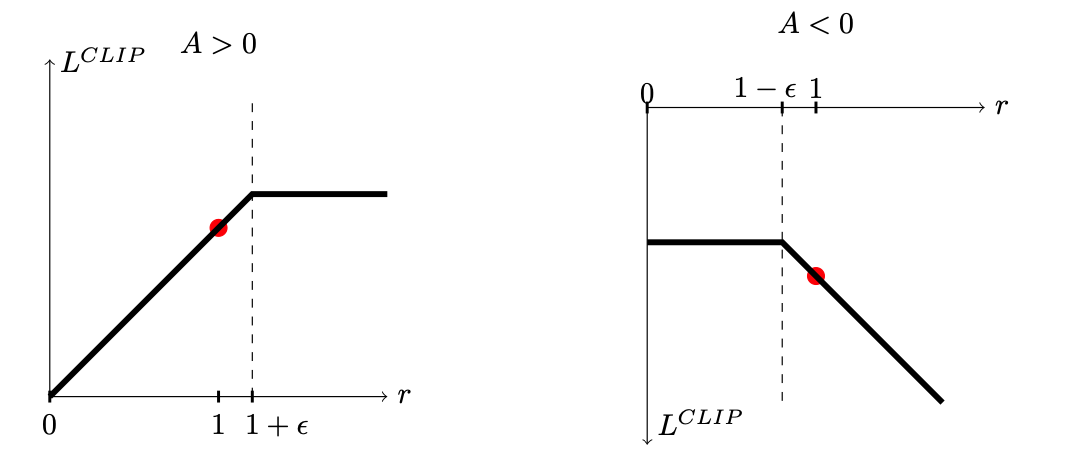
\includegraphics[width=0.8\linewidth]{images/ppo_lclip.png}
    \caption{Plots showing one term (i.e a single timestep) of the surrogate function $L$ as a function of the probability ratio $r$, for positive advantages left and negative advantages right, from \cite{schulman2017proximalpolicyoptimizationalgorithms}}
    \label{ppo_lclip}
\end{figure}
When the advantage is positive meaning the action we took lead to a better value then we would want the
policy to do more of this actions but the clipping in this case lets us not go beyond the $1+\epsilon$ ratio. When 
the advantage is negative meaning the action was less than favourable then there has to be at minimum a punishment of 
$1-\epsilon$ but there is no lower bound to it. 
\begin{algorithm}[H] 
\caption{PPO-Clip (OpenAI’s Spinning Up version \cite{OpenAI_Spinning_UP})} \label{alg:PPO-Clip} 
\begin{algorithmic} 
\STATE Input: initial policy parameters $\theta_0$, initial value function parameters $\phi_0$ 
\FOR{$k = 0,1,2,...$} 
\STATE Collect set of trajectories ${\mathcal D}_k = \{\tau_i\}$ by running policy $\pi_\text{old} = \pi(\theta_k)$ in the environment. 
\STATE Compute rewards-to-go $\hat{R}_t$. 
\STATE Compute advantage estimates, $\hat{A}_t$ (using any method of advantage estimation) based on the current value function $V_{\phi_k}$. 
\STATE Update the policy by maximizing the PPO-Clip objective: 
\begin{equation*} \theta_{k+1} = \arg \max_{\theta} \frac{1}{|{\mathcal D}_k| T} \sum_{\tau \in {\mathcal D}_k} \sum_{t=0}^T 
\min\left( \frac{\pi_{\theta}(a_t|s_t)}{\pi_{\theta_\text{old}}(a_t|s_t)} A^{\pi_{\theta_\text{old}}}(s_t,a_t), \;\; g(\epsilon, A^{\pi_{\theta_\text{old}}}(s_t,a_t))
\right), 
\end{equation*} typically via stochastic gradient ascent with Adam. 
\STATE Fit value function by regression on mean-squared error: 
\begin{equation*} \phi_{k+1} = \arg \min_{\phi} \frac{1}{|{\mathcal D}_k| T} \sum_{\tau \in {\mathcal D}_k} \sum_{t=0}^T\left( V_{\phi} (s_t) - \hat{R}_t \right)^2, 
\end{equation*} typically via some gradient descent algorithm. 
\ENDFOR \end{algorithmic} \end{algorithm}
PPO shows very impressive results, but there are many additional hacks needed to make it really perform well,
to list some: Value function clipping, Reward scaling, orthogonal initialisation, Adam learning rate annealing, reward clipping, 
observation normalisation, observation clipping, hyperbolic tan activations, Global gradient clipping

\subsection{Differentiable Trust Region Layers}
Recent work has shown that convex optimization problems can be embedded as differentiable layers within neural 
networks \cite{agrawal2019differentiableconvexoptimizationlayers}, enabling end-to-end training through optimization-
based components. Building on this idea, differentiable trust region layers enforce trust region constraints directly 
within the policy network \cite{otto2021differentiabletrustregionlayers}. This transforms what would otherwise be a 
complex constrained optimization problem into a standard differentiable layer that integrates seamlessly into deep 
reinforcement learning pipelines.

\subsection{Maximum Posteriori Optimization (MPO)}
MPO is the idea of Trust-Regions for Actor Critic Methods. MPO uses 2 steps to optimize the policy (inspired by Expectation Maximization)
\begin{itemize}
\item E-Step: Solve Trust Region problem for non-parametric distribution
\item M-Step: Weighted maximum likelihood using weights from E-step
\end{itemize}


\subsection{Self-Test Questions}
\begin{enumerate}
\sq{Why trust regions are important for policy gradients?}\newline Vanilla policy gradients suffer from the fact that he distance in parameter space does
not translate into policy space which can cause Overshooting (The update misses the reward peak and lands in a sub- optimal policy region) or Undershooting (Taking needlessly small steps in the gradient direction causes slow convergence). Trust regions introduces a constraint to the objective such that subsequent policies
do not have a high difference. 

\sq{Which divergence is typically used for the trust region and what are its properties?}\newline Typically the Kullback-Leiber-Divergence gets used which has the following properties \begin{itemize}
    \item always positive KL$(p||q)\geq 0$
    \item KL$(p||q) = 0 \iff p=q$
    \item Non-symmetric KL$(p||q)\neq$KL$(q||p)$
\end{itemize}

\sq{How does Lagrangian optimization work and why is it often easier to solve the dual than solving the primal objective.}\newline
For method see \ref{lagrangian_multipliers}. Solving the dual is often easier because maximizing $g(\lambda)$ is typically a convex optimization problem.

\sq{How to implement trust-regions with discrete actions using Lagrangian optimization?}\newline
We use lagrangian optimization to solve the optimization  objective
$$\argmax\limits_\pi \underset{a}{\sum}\pi(a)r(a),\quad
\text{ s.t. KL}(\pi(a)||q(a))\leq \epsilon,\underset{a}{\sum}\pi(a) =1 $$

\sq{How natural gradients are connected to trust regions?}\newline
Natural gradients approximates the Trust Region problem by using Taylor Expansion Approximation.

\sq{How the Fisher Information Matrix is used in the natural gradient algorithms?}\newline
The Fisher Information Matrix is used to approximate the KL divergence
$$\bar{D}_{KL}(\theta || \theta_k)  \approx \frac{1}{2} (\theta - \theta_k)^T F (\theta - \theta_k)$$

\sq{Why are natural gradients difficult to use for bigger networks?}\newline
The Fisher Informations Matrix is defined as (in the context of TRPO)
$$\underset{\pi_\theta}{\mathbb{E}}[\nabla_\theta \log{\pi_\theta(a|s)}{\nabla_\theta \log{\pi_\theta(a|s)}}^T]$$
The number of elements of that gradient is $|\theta|$ (in NN every weight) so the Fisher Informations Matrix is of dimension $|\theta|\times|\theta|$ 
%where $|\theta|$ are number of parameters. 
. For a DNN with millions of parameters this is very computational burden. 

\sq{What is the main idea of PPO (clipped version) and what are the benefits?}\newline The idea here is also to limit the gradient step according to the distance of the policies. But it does this without the KL constraint instead it clips the gradient if the ratio of the current and old policy is to big. This is much simpler to implement then TRPO and can be used with optimizers like ADAM.
\end{enumerate}

\subsection{Resources}
A short and easy-to-understand introduction to Lagrangian duality can be found in 
\cite{Lagrangian_Duality_for_Dummies}. There's also a great blog post about natural gradients by 
\cite{natural_gradients}. For learning about TRPO and PPO, the OpenAI Spinning Up series explains the 
ideas very clearly \cite{OpenAI_Spinning_UP}.
\section{Evolution Strategies}\label{evo_strats}
Traditional deep learning methods often rely on stochastic gradient descent (SGD) to optimize a given objective.
However, this approach assumes that gradients of the objective function are available — an assumption that doesn’t
always hold, especially when the function is non-differentiable or its analytic form is unknown.\newline 
Evolution Strategies (ES) offer an alternative: they are gradient-free, black-box optimization algorithms that can optimize 
objective functions without requiring explicit gradient information. This makes them particularly useful in settings where 
gradients are difficult or impossible to compute. Below is the general form of ES for optimizing $p_\theta(x)$:
\begin{enumerate}
    \item Generate a population of samples $D = \{(x_,f(x_i))\}$ where $x_i \sim p_\theta(x)$
    \item Evaluate the “fitness” of samples in $D$
    \item Select the best subset of individuals and use them to update $\theta$, generally based on fitness or rank. Go
    to 1
\end{enumerate}
In reinforcement learning (RL), episode-based algorithms often use black-box optimization techniques like ES to maximize the 
expected return of an entire trajectory — rather than focusing on step-by-step actions. This approach is particularly 
effective when dealing with sparse or non-Markovian reward structures, where traditional, step-based methods struggle.
Such an episode-based Task is for instance the Hopper task, where the goal is to jump as high as possible. Rewarding based on 
the current height (Markovian reward) would be less effective since height can fluctuate quickly. A better approach is to 
reward the agent based on the highest point reached during the episode, providing clearer guidance towards the desired 
behavior.\newline 
So the overall objective is to find a distribution $\pi_\theta(x)$ over variables $x\in \mathbb{R}^n$ that maximizes the 
expected value of the episodic return $R(\tau)$:
$$\theta = \argmax\limits_\theta \mathbb{E}_{\tau \sim \pi_\theta }[R(\tau)]$$
In this setting, Evolution Strategies (ES) can be used as a black-box optimizer to iteratively improve the policy parameters. 
The process typically follows these steps:
\begin{enumerate}
    \item Explore: sample parameters $\theta_i \sim p_k(\theta)$
    \item Evaluate: assess quality of parameters by generating trajectory $\tau_i \sim p_{\theta_i}(\tau) $ and define its quality through $g(\theta_i) = \mathbb{E}_{\tau \sim p_{\theta_i}(\tau)}[R(\tau)]$ 
    \item Update: compute new search distribution $p_{k+1}$
\end{enumerate}

\subsection{Gaussian Evolution Strategies}
In this section, we consider Evolution Strategies (ES) where the search distribution is modeled as a Gaussian. 
The goal is to learn the parameters of this distribution to efficiently explore the space of solutions. The complexity 
of the method depends on how expressive the Gaussian is:

\paragraph{First-order: Diagonal Gaussian search distribution}
Here, the Gaussian distribution is parameterized as follows:
$$p_\omega(\theta) = \mathcal{N}(\mu,\sigma^2I), \text{ with } \omega = \{\mu,\sigma\}$$
This variant is simple and highly scalable, making it suitable for high-dimensional problems. However, it uses an isotropic 
variance (i.e., the same in all directions), which often leads to slower convergence due to limited directional guidance 
during exploration.

\paragraph{Second-order: Full-Covariance Gaussian search distribution}
Here, the Gaussian distribution is parameterized as follows:
$$p_\omega(\theta) = \mathcal{N}(\mu,\Sigma), \text{ with } \omega = \{\mu,\Sigma\}$$
This allows for more flexible and efficient exploration by adapting the shape and orientation of the distribution 
through the covariance matrix. While it typically converges faster than the diagonal version, its computational 
cost scales poorly with dimensionality, making it less practical for very high-dimensional problems.

\subsubsection{ Canonical Evolution Strategy (CES)}
A basic first-order algorithm, using a diagonal Gaussian distribution, is the Canonical Evolutionary Strategy (CES). It 
updates only the mean $\mu$, keeping $\sigma$ fixed.
\begin{algorithm}[H]
   \large
    \caption{Canonical Evolutionary Strategy Algorithm}\label{ces}
    \begin{algorithmic}
    \STATE INPUT: $M \in \mathbb{N}$ number of elites 
    \STATE init. $w_i = \frac{\log{(M+0.5)}-\log{(i)}}{\sum_{j=1}^M \log{(M+0.5)}-\log{(j)}}$
    \REPEAT
    \STATE Sample $N$ parameter vectors $\theta_i\sim \mathcal{N}(\mu_k,\sigma^2 I)$
    \STATE Evaluate parameter vectors $g_i = g(\theta_i)$
    \STATE Sort $(\theta_i,\dots,\theta_N)$ according to $g_i$ (best ones come first)
    \STATE update $\mu$ ($\sigma$ is typically fixed): $$\mu_{k+1} = \mu_k + \sum_{i=1}^M w_i(\theta_i-\mu_k)= \sum_{i=1}^M w_i\theta_i$$
    \UNTIL Result is good enough
    \end{algorithmic}
\end{algorithm}

\subsubsection{Cross-Entropy Method (CEM)}
The Cross-Entropy Method (CEM) is one of the most popular second-order ES variants. It updates both the mean and the 
covariance matrix of the search distribution using elite samples.
\begin{algorithm}[H]
   \large
    \caption{Cross Entropy Method}\label{cem}
    \begin{algorithmic}
    \STATE INPUT: $M \in \mathbb{N}$ number of elites 
    \REPEAT
    \STATE Sample $N$ parameter vectors $\theta_i\sim \mathcal{N}(\mu_k,\Sigma_k)$
    \STATE Evaluate parameter vectors $g_i = g(\theta_i)$
    \STATE Sort $(\theta_i,\dots,\theta_N)$ according to $g_i$ (best ones come first)
    \STATE update mean :
    $$\mu_\text{elites} = \frac{1}{M}\sum_{i=1}^M\theta_i \qquad \mu_{k+1} = (1-\alpha)\mu_k+ \alpha\mu_\text{elites}  $$
    \STATE update covariance: 
    \begin{gather*}
        \Sigma_\text{elites} \frac{1}{M}\sum_{i=1}^M (\theta_i -\mu_\text{elites})  (\theta_i -\mu_\text{elites})^T \\
        \Sigma_{k+1} = (1-\alpha)\Sigma_k + \alpha \Sigma_\text{elites}
    \end{gather*}
    \UNTIL Result is good enough
    \end{algorithmic}
\end{algorithm}
However both these methods have some key limitations:
\begin{itemize}
    \item Lack of a clear optimization objective: Since they rely on ranking the candidates rather than directly optimizing 
    the expected reward, they do not explicitly maximize the expected return
    \item Monotonic weighting transformation: The method's ranking approach is monotonic, which can result in convergence to a 
    local optimum, especially in deterministic environments.
    \item Challenges in stochastic settings: In environments with stochastic rewards, the behavior of ranking-based methods 
    becomes less predictable and harder to analyze.
\end{itemize}
 
\subsection{Trust-Region Methods for Stochastic Search}\label{trust_regions_es}
One issue with approaches that iteratively update the search distributions is that the updates can either be too moderate or 
too greedy, often leading to suboptimal behavior. To address this, we can introduce the concept of trust regions, which we 
encountered in a previous section and constrains the updates in a way that avoids drastic changes, promoting more stable 
learning. In this case, the objective is defined as:
$$\theta = \argmax\limits_\theta \mathbb{E}_{\tau \sim \pi_\theta }[R(\tau)] \text{ s.t. } KL(p||p_\text{old}) \leq 
\epsilon$$
This can then be solved using Lagrange multipliers, yielding a closed-form solution for the search distribution. For a more 
detailed explanation and an alternative method involving trust regions, refer to \cite{JMLR:v25:22-0564}.

\subsection{Self-Test Questions}
\begin{enumerate}
\sq{What the advantages/disadvantages of an episode-based RL formulation are} 
\begin{itemize}
    \item[] + Clear Objective Definition: the agent's goal is often clearly defined in terms of episodes
    \item[] + Non-Markovian Rewards: can be more intuitive and better aligned with the overall task goals.
    \item[] - Delayed Feedback: In some tasks, the consequences of an agent's actions may not be immediately apparent, leading to delayed rewards.
\end{itemize}

\sq{ How episode-based RL is connected to black-box optimization / evolutionary strategies (ES)}\newline

\sq{ How we can use search distributions for black-box optimization} \newline
A search distribution is a probabilistic model used to sample candidate solutions to the black-box objective 
function. The idea is to treat the problem as one of searching for the optimal set of parameters (or 
solutions) by sampling from a distribution, then refining the distribution based on feedback (evaluations of 
the objective function aka black box).

\sq{ What is the difference between first-order and second order methods for optimizing search distributions? Pros/Cons?}\newline The difference is w.r.t. the complexity of the gaussian search distribution.
\begin{itemize}
    \item first-order : $ \mathcal{N}(\mu,\sigma^2I)$ (better for high dimension, converges slowly)
    \item second order : $ \mathcal{N}(\mu,\Sigma)$ (fast convergence, more directed exploration in parameter space, computable inefficient for high dimensions)
\end{itemize}

\sq{ How a simple policy gradient algorithm for the episode-based case looks like}\newline

\sq{ What are the qualitative differences to “deterministic” gradient descent using finite differences}\newline

\sq{ Why most ES use rankings instead of the fitness values}\newline
Evolutionary Strategies (ES) often use rankings instead of raw fitness values to avoid issues like noise, 
outliers, or scaling problems in the fitness function. Rankings are less sensitive to extreme fitness values, 
ensuring that the selection process is more stable and robust.

\sq{ How does the cross-entropy method work and what is it connection to evolutionary strategies}\newline
See algorithm \ref{cem}. CEM can be viewed as a special case of evolutionary strategies, particularly in its 
use of a population-based search and selection mechanism. Instead of using a simple mutation-based update as 
in ES, CEM updates the search distribution based on the best-performing candidates. 

\sq{ How to use trust-regions in for episode-based RL?}\newline
See \ref{trust_regions_es}

\sq{ Why can we use exact trust regions in this case (as opposed to Lecture 6)?}\newline
Because for Gaussian distributions there is a closed form solution of the KL-Divergence which does not require sampling
\end{enumerate}

\subsection{Resources}
A great resource on Evolution Strategies is the blog post by Weng (2019) \cite{weng2019ES}.
\section{Bayesian Optimization}
This section provides a simplified understanding of Bayesian Optimization (BayesOpt) and is not intended to be a detailed 
treatment of the topic. A comprehensive explanation would require additional concepts and methods that are beyond the scope of 
this discussion.\newline 
BayesOpt is another method designed for black-box, derivative-free global 
optimization. This means it is tailored for optimization problems where the objective 
function is unknown, complex, or cannot be directly analyzed (black-box), and or where 
derivatives are unavailable or difficult to compute (derivative-free).\newline 
Rather than directly optimizing the objective function, BayesOpt relies on a probabilistic surrogate model, typically a 
Gaussian Process (GP) to approximate the function's behavior. This surrogate model helps guide the search for the optimal 
solution. BayesOpt is particularly focused on global optimization, meaning it seeks the best solution across the entire search 
space rather than just local optima.\newline 
Through an acquisition function, BayesOpt strikes a balance between exploration (sampling areas with high uncertainty) and exploitation (focusing on areas that are already promising), making it an efficient approach when function evaluations are expensive or time-consuming. But it is limited by the number of dimensions (mostly $\leq$ 20) since it is 
very computational expensive. 

%Before going more in detail we will look at Bayes-theorem:
%$$\underbrace{p(\theta|D)}_\text{posterior} = \frac{\overbrace{p(D|\theta)}^\text{data likelihood}\overbrace{p(\theta)}^\text{prior}}{\underbrace{p(D)}_\text{evidence}}$$
%\begin{itemize}
%    \item prior: encodes our subjective belief 
%    \item posterior: Probability of parameter vector given the data
%    \item likelihood : Specified by our parametric model $D$
%    \item evidence: Normalization, can be used for model comparison
%\end{itemize}

\subsection{Surrogate Model (Gaussian Process Regression)}
In Bayesian optimization, the surrogate model is typically constructed using Gaussian Process (GP) regression, a Bayesian 
statistical approach. A GP model treats function values as random variables, assuming a prior distribution that is 
multivariate normal, characterized by a mean vector and a covariance matrix. The mean vector is computed by evaluating a mean 
function $\mu_\theta$ at each sampled input point $x_i$, while the covariance matrix $\Sigma_\theta$ is determined using a 
kernel function. This kernel encodes our belief that input points closer together in the input space are likely to have 
similar function values. The kernel is crucial as it dictates the correlation between points in the function's input space.

\subsection{Acquisition Function}
The acquisition function is central to guiding the optimization process. It decides where to evaluate next by balancing 
exploration (sampling in areas of high uncertainty) and exploitation (focusing on areas where the model predicts good 
outcomes). Popular acquisition functions include Upper Confidence Bound (UCB), Knowledge Gradient, Entropy Search, and 
Predictive Entropy Search, among others.\newline 
For instance, the UCB (Upper Confidence Bound see \ref{UCB}) acquisition function is a widely used strategy. 
It combines the predicted mean $\mu(x)$ from the Gaussian Process with the uncertainty $\sigma(x)$ at each point. The UCB 
function is defined as:
$$\text{UCB}(x) = \mu(x) + \sqrt{\beta} \cdot \sigma(x)$$
The goal is to maximize the UCB function to find the next point that either has high predicted values (exploitation) or high 
uncertainty (exploration). To identify the next point $x_\text{next}$ for evaluation, the acquisition function is optimized 
over the input space:
$$x_{\text{next}} = \arg \max_x \text{UCB}(x)$$

\subsection{Optimization Loop}
The optimization process proceeds iteratively. In each iteration:
\begin{itemize}
\item A new input point is selected based on the acquisition function.
\item The objective function is evaluated at that point.
\item The surrogate model (e.g., Gaussian Process) is updated with the new data.
\end{itemize}
The loop continues until a predefined stopping criterion is met, such as reaching a maximum number of iterations, 
exceeding a time limit, or observing negligible improvement in the objective function.

\subsection{Self-Test Questions}
\begin{enumerate}

\sq{Why we do we use a Bayesian treatment for learning the fitness function?}\newline
Bayesian methods allow for efficient optimization of expensive, noisy, or unknown functions 
by using a probabilistic model (e.g., Gaussian Process) to capture uncertainty and guide the 
search for optimal points without needing derivative information.

\sq{What a GP is and how to obtain the GP posterior}\newline
A Gaussian Process (GP) is a probabilistic model that defines a distribution over functions. 
The posterior is obtained by updating the prior distribution with observed data using Bayes' 
rule, resulting in a model that reflects the updated beliefs about the function.

\sq{How to use acquisition functions in BO?}\newline
Acquisition functions guide where to sample next. They balance exploration (uncertain 
regions) and exploitation (promising regions), commonly using Expected Improvement (EI) or 
alternatives like Knowledge Gradient (KG).

\sq{Why BO can give you the global maximum instead of just a local one?}\newline
BO uses a probabilistic model (GP) to model uncertainty and avoid local optima by selecting 
points that provide the most information, thus increasing the likelihood of finding the 
global maximum.

\sq{Difference between considering the exploration-exploitation tradeoff and pure 
exploration phase.}\newline
Exploration-exploitation balances uncertainty and predicted value, improving efficiency. 
Pure exploration focuses solely on areas with high uncertainty, which can be useful early in 
optimization but may not lead to the best result.

\sq{The key ideas of the acquisition functions}\newline
Acquisition functions guide the optimization by quantifying the tradeoff between 
exploring uncertain areas and exploiting known good areas to maximize the objective.

\sq{How to deal with hyper-parameters of the GP}\newline
Hyperparameters (e.g., length scale) are learned through maximum likelihood estimation or 
Bayesian inference to best fit the GP model to the observed data.

\sq{What are the pros and cons of BO in comparison to Stochastic Search?}
\begin{itemize}
\item Pros of BO: Efficient with fewer evaluations, good for expensive functions, global 
optimization.
\item Cons of BO: Computationally intensive for high dimensions.
\item Stochastic Search pros: Simple and scalable for high dimensions, no model required.
\item Cons of Stochastic Search: Less efficient for expensive functions, risk of local optima.
\end{itemize}
\end{enumerate}





\section{Planning}
In the previous sections, we focused on model-free algorithms (expect dynamic programming), where we \textbf{learned} policies or value 
functions by interacting with the environment, without any explicit model. Now, we shift to model-based settings, where we assume 
either that we can learn a model of the environment or are provided with one.\newline
\textbf{Planning} refers to any computational process that uses a model to produce or 
improve a policy for interacting with the modeled environment. We have already encountered 
planning in the context of value and policy iteration (Section \ref{dynammic programming}). 
In the following, we assume a model is available and explore various planning algorithms. 
(The next chapter will address how a model can potentially be learned.)

\subsection{Open-/Closed-Loop Planning}
In planning, we distinguish between open-loop and closed-loop planning.
In open-loop planning, the environment provides no feedback during execution. We are given 
an initial state and must immediately output a sequence of actions. For deterministic dynamics
this corresponds to solving an optimization problem to find the sequence of actions that maximizes the 
return :
$$a_1,\dots,a_T = \argmax\limits_{a_1,\dots,a_T} \underset{t=1}{\sum^T}r(s_t,a_t)\text{ s.t. } s_{t+1} = p(s_t,a_t)$$
In an environment with stochastic dynamics the optimization is stated as 
\begin{gather*}
    a_1,\dots,a_T = \argmax\limits_{a_1,\dots,a_T} \mathbb{E}\left[\underset{t=1}{\sum^T}r(s_t,a_t) \middle| a_1,\dots,a_T \right] 
    \quad s_{t+1} \sim p(s_{t+1}|a_t,s_t) \\
    \text{with } p(s_1,\dots,s_{T+1}|a_1,\dots,a_t) = p(s_1) \underset{t=1}{\prod^T p(s_{t+1}|a_t,s_t)} 
\end{gather*}
In open-loop planning, trajectories in stochastic environments are often suboptimal. Consider the analogy of taking an exam. Let’s say state 
$s_1$ represents the moment you receive the exam. The planned action sequence, in this case, corresponds to the answers you are going to give 
despite not knowing what the questions will be. Even if you're well-prepared, your answers are likely to be wrong, resulting in suboptimal 
outcomes since you can not look into the future. The fundamental problem is that open-loop plans cannot adapt to unexpected events or changes 
in the environment.We've already discussed open-loop methods like Random Shooting, Cross-Entropy Method (CEM), CMA-ES in section 
\ref{evo_strats}.\newline
In contrast, closed-loop planning allows the environment to provide feedback. In this 
setting, you’re given a state and asked to produce an action. After taking the action, the 
environment updates and returns the next state, continuing the cycle. This feedback loop 
enables more adaptive decision-making, as actions can be adjusted based on the state 
transitions and rewards observed during execution.
\begin{figure}[H]
    \centering
    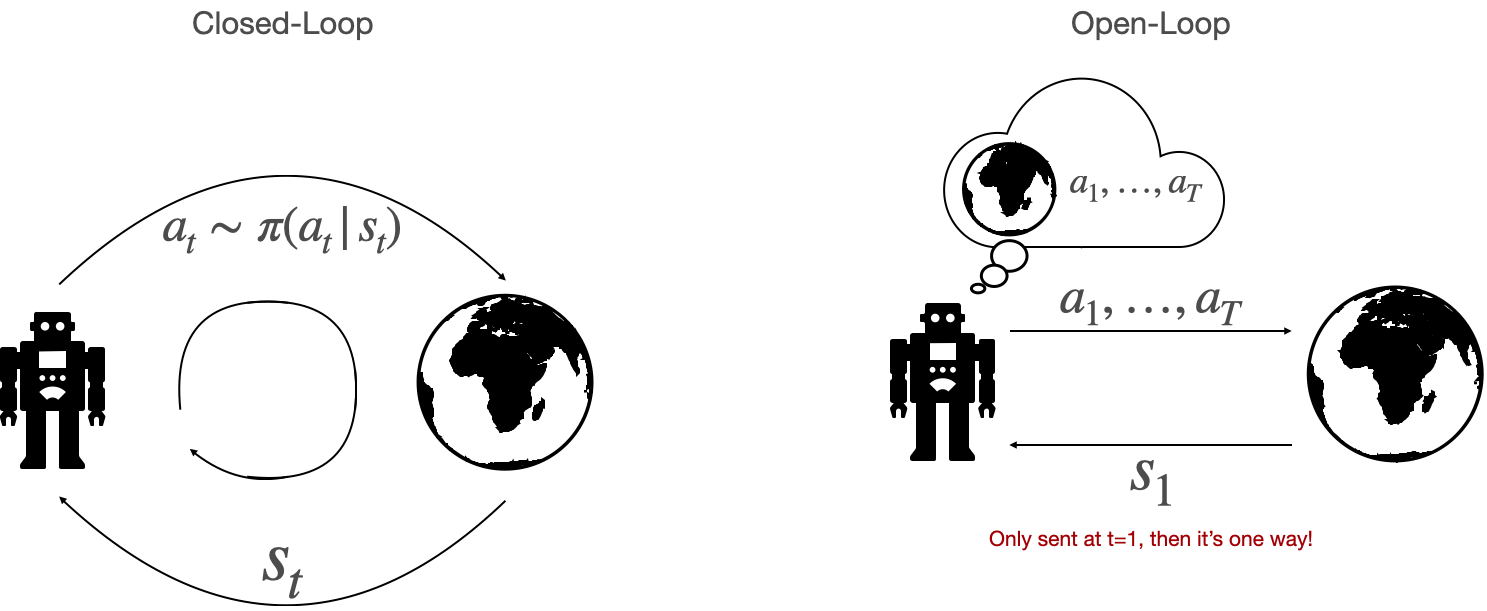
\includegraphics[width=0.9\linewidth]{images/closed_open_loop.png}
    \caption{Illustration of open- and closed-loop planning, inspired from ''CS 285: Lecture 10`` \cite{CS285,CS285LevineYoutube}}
    \label{fig:open_closed_loop}
\end{figure}

\subsection{Closed-Loop Planning in Discrete Domains - Monte-Carlo Tree Search}
For discrete domains, we have already explored dynamic programming approaches to derive 
policies given a model. However, in scenarios where the state space is large (e.g., Go, 
Chess, Atari, etc.), such methods become infeasible. An alternative is to use traditional 
tree search algorithms, but these also face limitations. For environments with huge 
branching factors, the search tree grows exponentially, making it computationally 
expensive.\newline
%Furthermore, tree search algorithms don't naturally handle stochastic transitions well.\newline
The approach we will be looking at next focuses on incrementally and asymmetrically building the 
search tree. Monte Carlo Tree Search (MCTS) addresses this by concentrating on the most 
promising moves and expanding the search tree through random sampling of the search space. 
MCTS consists of four main stages:
\begin{enumerate}
    \item \textbf{Selection:} start from root R and select successive child nodes until a leaf node L is reached. The root is the current game state and a leaf is any node from which no simulation (playout) has yet been initiated. The decision which child to take next is determined by the highest UCB-Score \ref{UCB}
    
    \item \textbf{Expansion:} unless the leaf L ends the game decisively (e.g. win/loss/draw) for either player, create one (or more) child nodes and choose node C from one of them. Child nodes are any valid moves from the game position defined by L. 
    
    \item \textbf{Simulation:} complete one random playout from node C. This step is sometimes also called playout or rollout. The rollout is typically performed with a default policy $\pi_\theta$. A playout may be as simple as choosing uniform random moves until the game is decided (for example in chess, the game is won, lost, or drawn).
    
    \item \textbf{Backpropagation} use the result of the playout to update information in the nodes on the path from C to R. For 1-0 (win-loss games), that means updating the win-loss counts of all the ancestor nodes. Note that the win count updates alternate between 0 or 1 (e.g. for black-white players) as you go up the tree.
\end{enumerate}
\begin{figure}[H]
    \centering
    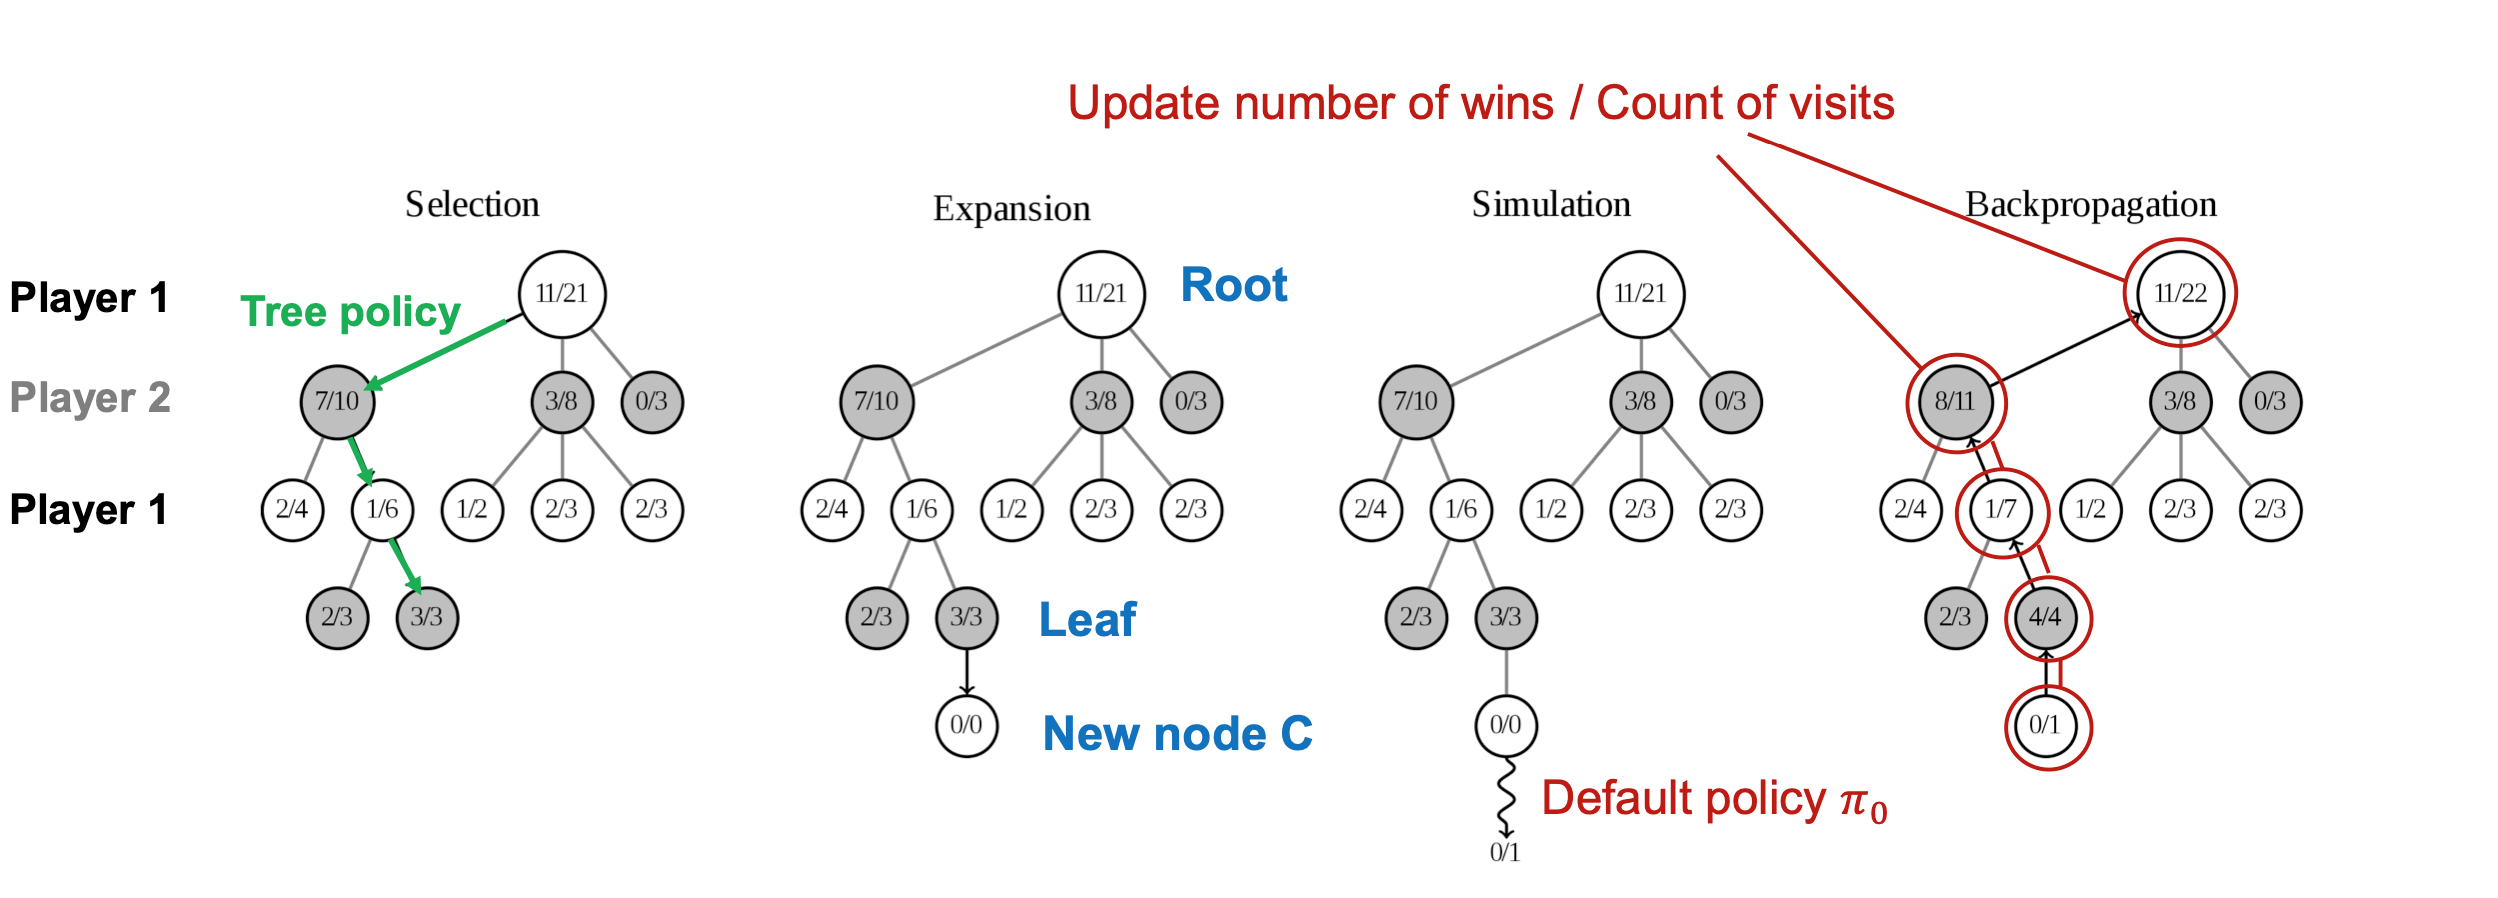
\includegraphics[width=\linewidth]{images/MCTS.png}
    \caption{The different phases of MCTS, image from KIT }
    \label{fig:MCTS}
\end{figure}
However, a major challenge arises when using Monte Carlo Tree Search (MCTS) in environments with continuous state and action spaces. In such 
cases, MCTS becomes significantly harder to apply effectively, as it's highly unlikely to encounter exactly the same states during planning.
This makes it difficult to build and reuse a meaningful search tree. To address this issue, we will explore an alternative method that is 
better suited for planning in continuous domains in the following chapter. But before we do that, we will first take a closer look at how 
MCTS has been used for planning in reinforcement learning.

\subsubsection{Alpha-Go and it successors}
\paragraph{AlphaGo} combined deep neural networks with Monte Carlo Tree Search (MCTS) and was trained using a combination of supervised 
learning from expert human games and reinforcement learning through self-play. It used separate networks to predict the best move (policy) 
and the likely winner (value).
\paragraph{AlphaGo Zero} is the successor to AlphaGo. AlphaGo Zero learned entirely from scratch, using only self-play without any human 
data. It also simplified the architecture by using a single neural network to predict both the policy and value, making it not only more 
efficient but also more powerful. This version surpassed the original AlphaGo despite having no prior knowledge of human strategies. 
\paragraph{AlphaZero}  generalized the approach from AlphaGo Zero. It used the same learning framework as AlphaGo Zero but was applied to 
different games, including Chess, Shogi, and Go. AlphaZero learned purely through self-play and used MCTS alongside a neural network, just 
like AlphaGo Zero, but it demonstrated that this method could be adapted to multiple environments with known rules.
\paragraph{MuZero} was the next major advancement. While AlphaZero still required a perfect simulator or full knowledge of the environment's 
rules, MuZero removed this assumption entirely. It learned not just the policy and value function, but also an internal model of the 
environment's dynamics—enabling planning without access to the real rules. Instead of learning to predict exact future states, MuZero learned 
a compact latent representation, from which it could plan and estimate rewards, values, and future outcomes.
\paragraph{AlphaTensor} was designed to discover new algorithms instead of learning to play games like Chess or Go. Specifically, it learns 
to find efficient matrix multiplication algorithms by framing the task as a single-player reinforcement learning problem.


A nice visualisation of how MCTS works and how it got used in AlphaZero/Go can be found \href{http://joshvarty.github.io/AlphaZero/}{here}.

\subsection{Resources}
Much of the content presented here is based on Sergey Levine’s CS 285: Lecture 10 \cite{CS285,CS285LevineYoutube}.
A helpful visualization of how Monte Carlo Tree Search (MCTS) works, particularly in the context of AlphaZero can be 
found on \cite{alphaZero}. For a technical breakdown of AlphaGo see the article \cite{alphaGo}, and for an overview 
of MuZero refer to DeepMind’s blog post \cite{muZero}.

\section{Model Predictive Control / Closed-Loop Planning in Continuous Domains – Optimal Control}
Model Predictive Control (MPC) is an optimal control strategy designed for managing complex systems, particularly 
those with constraints. At its core, MPC relies on predicting the system’s future behavior and using this prediction 
to determine the optimal action at the current time step. As new data becomes available, the controller updates its 
plan, making MPC well-suited for dynamic and uncertain environments. The process unfolds as follows:
\begin{enumerate}
    \item \textbf{Model of the System:} MPC begins with a mathematical model that describes how the system evolves in response to different 
    inputs.
    \item \textbf{Prediction Horizon:} At each time step, the controller uses the model to predict the system’s future behaviour over a fixed 
    time window, known as the prediction horizon. It simulates how the system would respond to different control inputs over this period.
    \item \textbf{Optimization Problem:} The controller then formulates and solves an optimization problem to find the optimal sequence of 
    control actions over the prediction horizon. This sequence is chosen to minimize a predefined cost function.
    \item \textbf{Apply Only the First Action:} Instead of applying the entire sequence, MPC executes only the first action from the 
    optimized plan. After this step the system state is then updated, and the process repeats.
\end{enumerate}
By continuously updating its decisions in this way, MPC can react to unexpected changes and uncertainties in the environment. In the 
following  we will explore how to solve such optimization problems (step 3) in different settings. We will focus on finite-horizon problems without 
constraints. Before we begin, we’ll introduce some standard notation from optimal control theory and clarify how it relates to terms commonly 
used in reinforcement learning (RL):
\begin{itemize}
    \item $x$ represents the state of the system ($s$).
    \item $u$ represents the control input or action ($a$).
    \item $c(x,u)$ is the cost function, which is the counterpart to the reward function in RL (note that RL typically maximizes reward, while control minimizes cost)
    \item $f(x,u)$ defines the system dynamics, describing how the state evolves. This corresponds to the transition function or transition probabilities in RL.
\end{itemize}

\subsection{Linear Quadratic Regulator}
We will start by looking at the Linear Quadratic Regulator (LQR). In LQR, "linear" refers to 
the system dynamics being linear, and "quadratic" refers to the cost function being 
quadratic. A typical LQR problem can be formulated as:
\begin{gather*}
    \min\limits_{u_1,\dots,u_T} c(x_1,u_1)+c(f(x_1,u_1),u_2)+\dots+c(f(f(\dots)\dots),u_T) \\
    f(x_t,u_t) = F_t
\begin{bmatrix} 
x_t\\ u_t 
\end{bmatrix}
 + \mathbf{f} \qquad 
 c(x_t,u_t) = \frac{1}{2} \begin{bmatrix} 
x_t\\ u_t 
\end{bmatrix}^T C_t \begin{bmatrix} 
x_t\\ u_t 
\end{bmatrix}+ \begin{bmatrix} 
x_t\\ u_t 
\end{bmatrix}^T \mathbf{c}_t
\end{gather*}
To find the optimal sequence of actions, we minimize the cost function over time. The details of how to solve this can 
be found in the recommended resources. However, LQR is limited to systems with deterministic and linear state transitions.

\subsection{Linear–quadratic–Gaussian Control}
When dealing with stochastic transitions, we extend the LQR framework to the Linear Quadratic Gaussian (LQG) model. The overall problem 
formulation remains the same as in LQR, with the key difference being how we define the system dynamics. In LQG, transitions are modeled as 
linear functions with additive Gaussian noise:
$$p(x_{t+1}|x_t,u_t) = \mathcal{N}( F_t
\begin{bmatrix} 
x_t\\ u_t 
\end{bmatrix}
 + \mathbf{f}, \Sigma_t)$$
In other words, we take the deterministic transition function from LQR and simply add Gaussian noise to account for uncertainty. The good 
news is that the same algorithm used to solve the LQR problem can also be applied to the LQG setting. 

\subsection{Approximating Non-Linear Systems (iLQR)}
While LQR and LQG are effective for linear systems, real-world systems are often non-linear and require a different approach. To handle non-
linear dynamics, we can approximate both the dynamics and the cost function locally using a Taylor expansion around the current trajectory 
point $(\hat{x}_t,\hat{u}_t)$.
 \begin{gather*}
     f(x_t,u_t) \approx  f(\hat{x}_t,\hat{u}_t)+ \nabla_{x_t,u_t} f(\hat{x}_t,\hat{u}_t) \begin{bmatrix} 
x_t- \hat{x}_t\\ u_t- \hat{u}_t 
\end{bmatrix} \\
c(x_t,u_t) = c(\hat{x}_t,\hat{u}_t) + \nabla_{x_t,u_t} c(\hat{x}_t,\hat{u}_t) \begin{bmatrix} 
x_t- \hat{x}_t\\ u_t- \hat{u}_t 
\end{bmatrix}+
\frac{1}{2} \begin{bmatrix} 
x_t- \hat{x}_t\\ u_t- \hat{u}_t 
\end{bmatrix}^T 
\nabla_{x_t,u_t}^2 c(\hat{x}_t,\hat{u}_t)
\begin{bmatrix} 
x_t- \hat{x}_t\\ u_t- \hat{u}_t 
\end{bmatrix}
 \end{gather*}
 we then define 
$$ \bar{f}(x_t,u_t) = \underbrace{F_t}_{ \nabla_{x_t,u_t} f(\hat{x}_t,\hat{u}_t)}
\begin{bmatrix} 
x_t\\ u_t 
\end{bmatrix}
 + \mathbf{f} \qquad 
 \bar{c}(x_t,u_t) = \frac{1}{2} \begin{bmatrix} 
x_t\\ u_t 
\end{bmatrix}^T \underbrace{C_t}_{\nabla_{x_t,u_t}^2 c(\hat{x}_t,\hat{u}_t)} \begin{bmatrix} 
x_t\\ u_t 
\end{bmatrix}+ \begin{bmatrix} 
x_t\\ u_t 
\end{bmatrix}^T \underbrace{\mathbf{c}_t}_{\nabla_{x_t,u_t} c(\hat{x}_t,\hat{u}_t)}$$
With these approximations, we effectively transform the non-linear control problem into a locally linear-quadratic one, which we can now 
solve using the standard LQR algorithm.

\subsection{Resources}
A more detailed explanation of Model Predictive Control and the solution to the equations above can be found in 
Sergey Levine’s CS 285: Lecture 10 \cite{CS285,CS285LevineYoutube}.

\section{Model-Based Reinforcement Learning (MBRL)}
All the algorithms we have looked at so far were either model-free, meaning that we 
had no model of the world and just learned value functions by interacting with the 
environment, or the dynamic programming approach, which assumes that we do have a 
model and can solve for the optimal solution without having to interact with the world. \newline
In model based reinforcement learning we learn a model from experience and use the 
learned model to do planning. By model we mean the transition probabilities/ dynamics. 
One way to learn the dynamics is to use equations of motion and then 
identify the parameters from the given data but this is not really scalable for 
complex systems. The more common approach is to use neural networks to learn the 
dynamics models. The most basic model based reinforcement learning 
algorithm would look like algorithm \ref{mbrl} where we use the experience $\{S_1,A_1,\dots,S_T\}$ 
and reduce it to a supervised learning problem.
\begin{algorithm}[H]
  \large
    \caption{Basic Model-Based RL}\label{mbrl}
    \begin{algorithmic}
        \FOR{$i=1,2,\dots$}
        \STATE collect data under the current policy
        \STATE learn dynamics model from past data
        \STATE improve policy by using dynamics model
        \ENDFOR
    \end{algorithmic}
\end{algorithm}
Model-based reinforcement learning (MBRL) offers several advantages, such as data 
efficiency, improved safety through simulation, and faster adaptation capabilities. 
However, the simple MBRL algorithm described in algortihm \ref{mbrl} also has some 
drawbacks. The problem arises from the circular dependency between data 
collection, model learning, and policy improvement. If any of these components perform 
poorly, everything can start to fail. This also introduces now two sources of approximation error: one 
from learning the model itself, and the other from using the learned model to derive the 
value function. There are many potential reasons for failure in any 
of these areas, but for now, we are focusing on the model learning aspect.

\subsection{Distributional shift}
One reason for bad performing policies which got trained by a learned model is 
distributional shift. Suppose we have trained a model on a given dataset of trajectories 
until it achieves low error on this data. However, since our model is not perfect, it will 
likely make small deviations from the true actions (e.g., slightly steering left) during 
testing. These errors accumulate over time, causing the model to encounter states it 
rarely or never saw during training. As a result, the model performs poorly on these 
unseen states.\newline
The core problem is that the state distribution on which the model was trained differs from the distribution the model generates 
during testing. Consequently, the model struggles to extrapolate to these new regions of the state space. One way to address this 
is by augmenting the training dataset with real dynamics tuples $(s,a,s')$ collected by executing the model’s own actions in the 
actual environment. This approach, which we will also revisit in the Imitation Learning chapter, helps the model adapt to the 
distribution it will face at test time.

\subsection{Model Exploitation}
The second challenge is model exploitation, a phenomenon related to overfitting, as depicted in Figure~\ref{model_exploit}. In 
this figure, the green curve represents the true Q-values, while the red curve shows the Q-values induced by the learned dynamics 
model. Since the model is used to calculate these Q-values, any inaccuracies in the model can lead to erroneous spikes in the 
predicted values. The policy, relying on these faulty predictions, may exploit these artifacts—choosing actions that appear 
optimal based on the model but are actually suboptimal or even harmful in the real environment. This can result in the policy 
overfitting to the inaccurate dynamics model (choosing this faulty spikes), leading the agent to take unrealistic actions and 
explore areas of the state space it has never encountered, ultimately causing a distributional shift.

\begin{figure}[H]
    \centering
    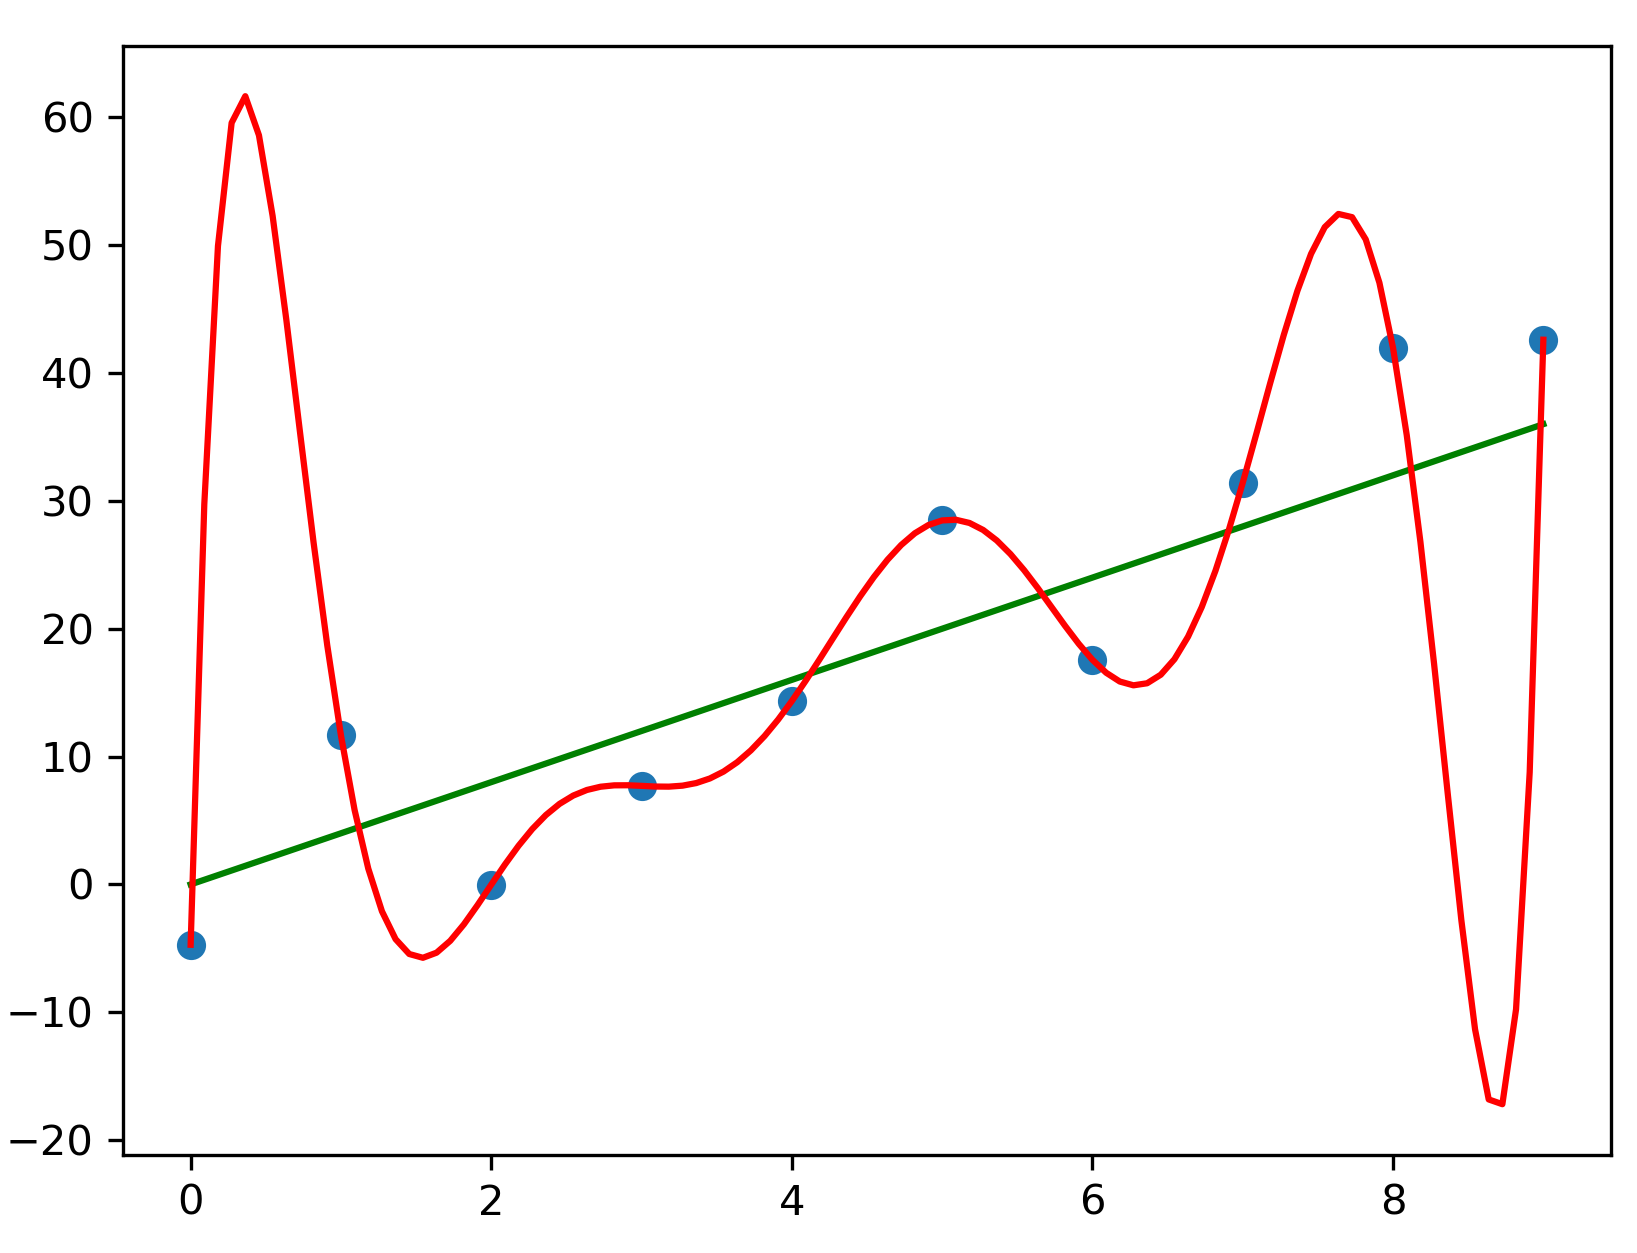
\includegraphics[width=0.5\linewidth]{images/Pyplot_overfitting.png}
  \caption{Illustration of overfitting: The green curve represents the true underlying function (ground truth), while the blue 
    dots are noisy samples drawn from it. The red curve shows the model's learned approximation, which fits the training data 
    closely but fails to generalize well. From \cite{wiki:xxx}.}
    \label{model_exploit}
\end{figure}

\subsection{Uncertainty}
One way to mitigate model exploitation is by incorporating uncertainty into the dynamics model. Rather than predicting a single 
next state for a given state-action pair, the model instead returns a distribution over possible next states. This allows the 
agent to evaluate actions based on their expected rewards while taking the uncertainty in the dynamics into account. By 
considering the full distribution of possible outcomes, the agent becomes less likely to overfit to inaccurate model predictions 
and is encouraged to choose actions that are more robust to uncertainty in the environment.
\begin{figure}[H]
    \centering
    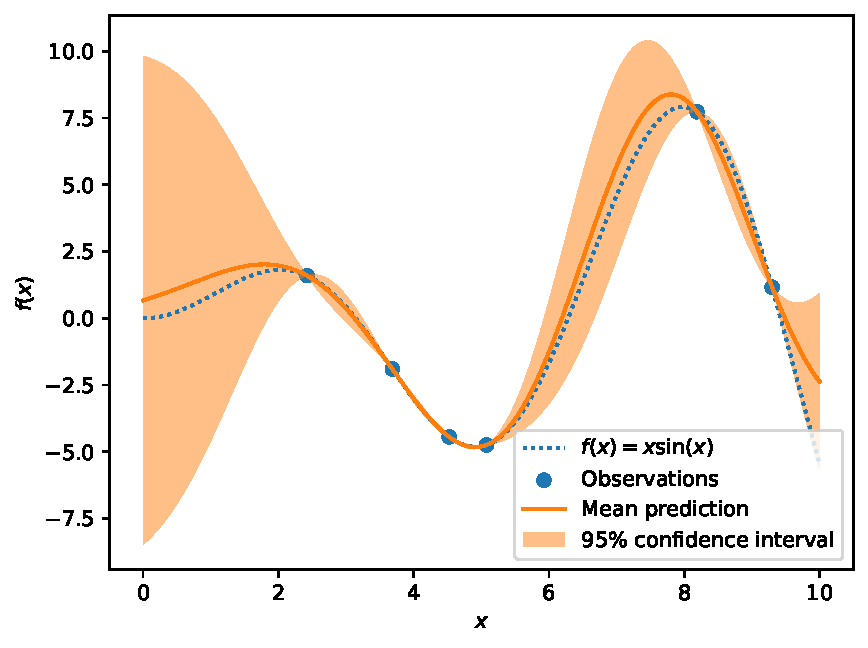
\includegraphics[width=0.7\linewidth]{images/gp_visual.pdf}
    \caption{ Gaussian process regression on noise-free dataset from \cite{GP}}
    \label{uncert_plot}
\end{figure}
However, there are several challenges with this approach. From earlier chapters, we know 
that exploration is crucial for discovering optimal policies. If our model is too 
pessimistic, it may avoid risky actions, leading to a lack of exploration. As a result, 
the agent might not discover better solutions or improve its policy. In the following 
sections, we will explore the different types of uncertainty and how we can mitigate their 
impact to encourage more effective exploration while still accounting for the uncertainty 
in the learned dynamics.

\subsubsection{Epistemic uncertainty}
Epistemic uncertainty refers to the uncertainty about the world due to a lack of 
experience (or data). This type of uncertainty can be reduced by gathering more data to 
improve our understanding. However, another approach to managing this uncertainty is to 
explicitly incorporate it into the models themselves.

\paragraph{Bayesian Learning}
Bayesian learning addresses epistemic uncertainty by treating model parameters as probabilistic rather than fixed. Instead of 
assigning a single value to each weight, we represent them as probability distributions—commonly Gaussians defined by a mean and 
variance. This probabilistic framework allows us to quantify how uncertain we are about the learned parameters. 

\paragraph{Ensembles}
Another simpler method to address epistemic uncertainty is by using an ensemble of models. 
Instead of training a single model, you train $k$ models, each of which learns the task 
independently. For prediction, we can then average the outputs of all models to obtain a 
more robust prediction.\newline
To ensure diversity among the models in the ensemble, it is helpful to train each model on 
independent training sets. This independence allows the models to explore different 
aspects of the problem and helps reduce the overall uncertainty in the predictions.

\subsubsection{ Aleatoric uncertainty}
Aleatoric uncertainty refers to the inherent uncertainty within a system, meaning that no 
matter how much experience or data you gather, some aspects will always remain uncertain. 
A classic example of aleatoric uncertainty is predicting the outcome of a dice roll. The 
outcome is uncertain, and no matter how many dice rolls you make, you can never predict 
the exact result with certainty using a deterministic function.\newline
In reinforcement learning, there are three primary sources of aleatoric uncertainty, each corresponding to a component of the Markov Decision Process (MDP):
\begin{itemize}
\item  Stochastic Rewards: When the reward function is stochastic, there is an irreducible 
uncertainty about the true value of the reward.
\item Stochastic Observations: Uncertainty in the observations received from the environment.
\item Stochastic Actions: When actions in the environment are uncertain, resulting in variability in outcomes even if the agent’s actions are deterministic.
\end{itemize}
To address aleatoric uncertainty, practitioners often use probabilistic neural networks, 
which can model this uncertainty explicitly by outputting a distribution over possible 
outcomes, rather than just point estimates. This approach allows the agent to account for 
inherent randomness in the environment and make better decisions under uncertainty.

\subsection{Replanning}
Since no learned model can perfectly predict the outcome of every action, one way to reduce the impact of model inaccuracies is 
through replanning. Unlike open-loop planning, which commits to a fixed sequence of actions and is prone to compounding errors, 
replanning continuously updates the plan based on new observations at each time step. This enables the agent to correct for past 
mistakes and adapt to changes in the environment. This strategy is commonly known as Model Predictive Control (MPC).

\subsection{Probabilistic Ensembles with Trajectory Sampling (PETS)}
PETS is a model-based reinforcement learning (MBRL) method introduced by \cite{chua2018deepreinforcementlearninghandful}. It 
represents a powerful approach to reinforcement learning by combining probabilistic modeling with planning. Rather than learning 
a policy directly, PETS simulates future outcomes using a learned model of the environment and chooses actions based on this 
simulated future.

\subsubsection{Core Components}
\begin{itemize} 
\item \textbf{Probabilistic Ensembles:}
PETS does not rely on a single neural network to model environment dynamics. Instead, it uses an ensemble of neural networks, 
each trained to predict the next state given the current state and action. These networks are probabilistic, typically outputting 
parameters of a Gaussian distribution over the next state. 

\item 
\textbf{Trajectory Sampling:}
Rather than only choosing the next action based on immediate predictions, PETS samples entire sequences of future trajectories. This is achieved by: 
\begin{itemize} 
\item Sampling multiple models from the ensemble. 
\item Simulating rollouts using these models over several timesteps. 
\item Sampling from the predicted distributions at each step (the models are probabilistic models so there outputs are 
distributions which we need to sample from in order to get the state). 
\item Evaluating the total expected reward of each trajectory. 
\end{itemize}

\item \textbf{Model Predictive Control (MPC):}
PETS uses the ensemble and trajectory sampling to perform planning at every timestep via MPC. The loop is as follows: \begin{itemize} 
\item Trajectory Sampling from the current state. 
\item Choose the sequence with the highest predicted reward. 
\item Execute only the \emph{first} action of the best sequence in the real environment. 
\item Observe the next state, update the model with new data, and repeat the process. 
\end{itemize} 
\end{itemize}

\begin{figure}[H]
    \centering
    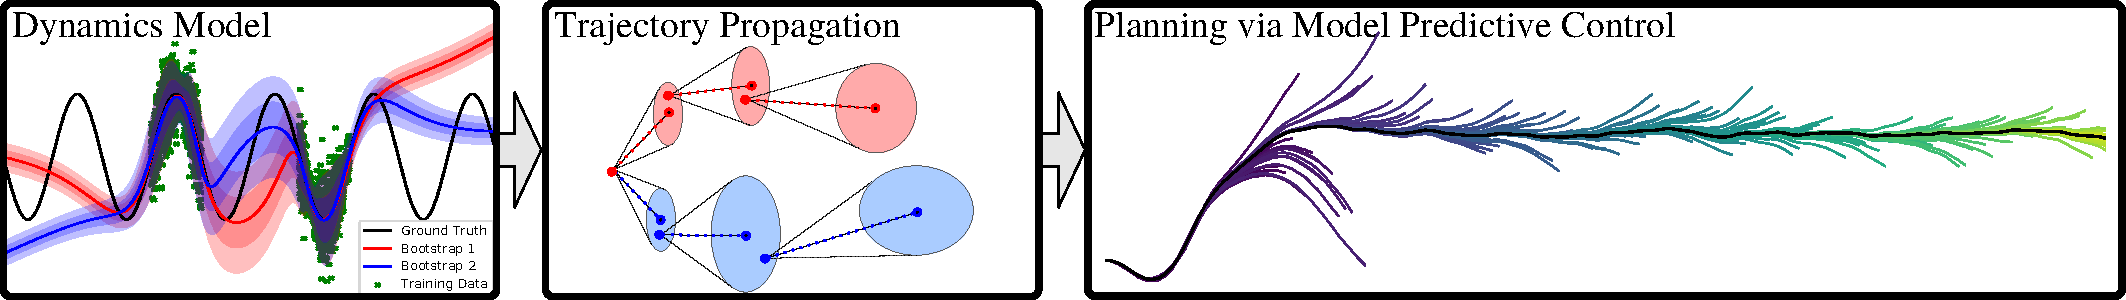
\includegraphics[width=\linewidth]{images/PETS.pdf}
    \caption{Illustration of the PETS method from \cite{chua2018deepreinforcementlearninghandful}.}
    \label{fig:PETS}
\end{figure}

\subsection{Model-Based Policy Optimization (MBPO)}
MBPO \cite{janner2021trustmodelmodelbasedpolicy} combines model-free and model-based reinforcement learning into a unified 
approach. While a dynamics model is learned from collected data, the policy is not limited to being trained exclusively in a 
model-free or model-based manner. Instead, MBPO leverages both real environment interactions and short model-generated rollouts 
to train the policy. As the agent interacts with the environment, new data is gathered to continually refine the learned model 
and improve policy performance.

\subsection{Model-Based-RL under Partial Observability}
Previous methods typically assume that environment dynamics can be represented as functions mapping state-action pairs to next 
states. However, this assumption relies on access to the true underlying states of the environment, which is often not the case 
in practice.\newline
This limitation becomes clear in image-based tasks, such as those found in Atari games. From a single image, 
it is generally impossible to directly infer latent properties like the velocity or direction of a moving object. In such cases,
the agent receives only partial observations (e.g., raw pixels), and the true state must be inferred.\newline
To address this challenge, we require a more general framework: the Partially Observable Markov Decision Process (POMDP). A POMDP 
extends the standard MDP formulation by modeling environments where the agent does not have full observability of the underlying 
state. Formally, a POMDP is defined by:

\begin{itemize}
    \item state space $S$ (not directly observable)
    \item action space $A$
    \item observation space $O$ (observable)
    \item transition model $p(s_{t+1}|s_t,a_t)$ (not known)
    \item reward function $r(s_t,a_t)$
    \item observation model $p(o_t|s_t)$
    \item initial state distribution $p(s_0)$
\end{itemize}
In general, POMDPs represent hidden Markov models, as illustrated in Figure 
\ref{pomdp_hmm}. If we knew the states $S$, the transition probabilities 
$p(s_{t+1}|s_t,a_t)$, the observation likelihoods $p(o_t|s_t)$ and if everything were 
Gaussian, we could compute the hidden states from the observations. This would allow us to 
apply the methods we've been using all along to learn policies. However, in reality, none 
of these assumptions typically hold.
\begin{figure}[H]
    \centering
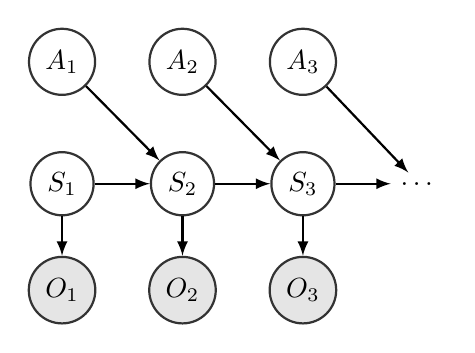
\begin{tikzpicture}
\tikzset{
  main/.style={circle, minimum size = 5mm, thick, draw =black!80, node distance = 7mm},
  connect/.style={-latex, thick},
  box/.style={rectangle, draw=black!100}
}
  \node[main] (L1) [] {$S_1$};
  \node[main] (L2) [right=of L1] {$S_2$};
  \node[main] (L3) [right=of L2] {$S_3$};
 % \node[main] (Lt) [right=40mmof L3] {$S_t$};
  \node[] (Lhid) [right=7mm of L3] {$\dots$};
  
\node[main] (A1) [above = of L1] {$A_1$};
\node[main] (A2) [above = of L2] {$A_2$};
\node[main] (A3) [above = of L3] {$A_3$};
%\node[main] (At) [below left=10mm of Lt] {$A_{t-1}$};


  \node[main,fill=black!10] (O1) [below=5mmof L1] {$O_1$};
  \node[main,fill=black!10] (O2) [below=5mmof L2] {$O_2$};
  \node[main,fill=black!10] (O3) [below=5mmof L3] {$O_3$};
  %\node[main,fill=black!10] (Ot) [below=of Lt] {$O_t$};
  \path (L1) edge [connect] (L2)
        (L2) edge [connect] (L3)
        (L3) edge [connect] (Lhid);
        %(Lhid) edge [connect] (Lt);
        
  \path (A1) edge [connect] (L2)
        (A2) edge [connect] (L3)
        (A3) edge [connect] (Lhid);
        %(At) edge [connect] (Lt);
  \path (L1) edge [connect] (O1);
  \path (L2) edge [connect] (O2);
  \path (L3) edge [connect] (O3);
  %\path (Lt) edge [connect] (Ot);
\end{tikzpicture}
    \caption{A POMDP illustrated as a hidden markov chain}
    \label{pomdp_hmm}
\end{figure}
A common approach in model-based reinforcement learning under partial observability is to first learn a mapping from high-
dimensional observations (e.g., images) to a lower-dimensional latent state space. This latent space is designed to capture the 
essential features of the environment needed for decision-making, even if it does not correspond directly to the true underlying 
state. To learn this mapping, Variational Autoencoders (VAEs) are typically used, providing both an encoder (from observation to 
latent state) and a decoder (from latent state back to observation). Once this representation is learned, the dynamics model is 
trained directly in the latent space.\newline 
There are several possible choices for modeling the encoder. The most accurate approach is to learn the posterior $q_\psi(s_t 
\mid o_{1:t}, a_{1:t})$, which incorporates the full history of observations and actions. However, while this posterior provides 
the most precise estimate of the latent state, it is also the most complex to learn. A simpler, though less accurate, alternative 
is to use a single-step encoder, which learns the posterior $q_\psi(s_t \mid o_t)$ based solely on the current observation. \newline
In recent years, several methods have been proposed that excel in model-based reinforcement learning. While a detailed discussion
is beyond the scope, here are some notable approaches:
\begin{itemize} 
\item PlaNet (introduced Recurrent State Space Models (RSSM) ) \cite{hafner2019learninglatentdynamicsplanning}
\item Dreamer (Dream to Control) \cite{hafner2020dreamcontrollearningbehaviors}
\end{itemize}

\subsection{Self-Test Questions}
\begin{enumerate}
\sq{ What is the difference between model-based and model-free RL?}\newline
In model-based RL, we learn a model of the environment and use it for planning. In model-
free RL, we don't focus on learning a model; instead, we learn value functions or policies 
by directly interacting with the environment.

\sq{Why is model learning in MBRL not just supervised learning?}\newline
In supervised learning, our data comes from a single underlying distribution $p$ and we 
aim to learn the mapping from features to labels. However, model learning in model-based 
RL (MBRL) is cyclic. We use the model to improve a policy, which then generates new data 
that is used to further optimize the model. This feedback loop results in a shifting 
distribution of data, so there is no fixed objective, unlike in supervised learning.

\sq{What are the different types of uncertainty, how can they be captured and why is that important for MBRL?} \newline
There are two primary types of uncertainty:
\begin{itemize}
    \item Epistemic uncertainty: This refers to the uncertainty about the world due to a 
    lack of data. It can be reduced by gathering more data or incorporating uncertainty 
    directly into the model (e.g., through Bayesian learning).
    \item Aleatoric uncertainty: This refers to uncertainty inherent in the system, meaning no matter how much data we gather, some uncertainty remains irreducible. This type of uncertainty can be captured by using probabilistic models.
\end{itemize}
Understanding and addressing these types of uncertainty is crucial in model-based 
reinforcement learning (MBRL). If uncertainty is not properly accounted for, it can lead 
to model exploitation, where the agent might overfit to the learned model and make poor 
decisions based on inaccurate predictions, ultimately impacting the performance of the 
policy.

\sq{How can you plan with an imperfect model?}\newline
One approach is replanning after each action is taken, turning an open-loop problem into a 
closed-loop process. This way, the agent can adjust based on new observations and model 
corrections.

\sq{What is partial observability, why is it important?}\newline
Partial observability occurs when we cannot fully observe the state of the environment. In 
many real-world scenarios, this happens due to missing sensor data or limited context 
(e.g., in image-based tasks like Atari, where a single image doesn’t provide information 
about the ball's velocity or direction). Since we can't directly observe the state, this 
complicates the use of algorithms that assume full observability.

\sq{What are the state space assumptions?}
\begin{itemize}
    \item observations only depend on the current state $p(o_t|s_t)$
    \item states depend only on the previous state and the action $p(s_{t+1}|s_t,a_t)$
\end{itemize}

\sq{How can we use Variational Inference to learn deep SSMs/sequential VAEs?}\newline

\sq{How can we use those for model based RL under partial observability?}\newline
Sequential VAEs and deep state-space models encode observations into a lower-dimensional 
latent space that represents the states. This latent space can then be used by a dynamics 
or inference model to predict future states, enabling planning and decision-making despite 
partial observability.

\sq{How can you use a model to learn a parametric policy?}\newline
A parametric policy can be learned by training policy networks and value-function networks 
on imagined or simulated trajectories generated by the learned model. These simulated 
trajectories provide a way to refine the policy without needing real-world data.

\end{enumerate}

\subsection{Resources}
Much of the general content presented here is based on Sergey Levine’s CS 285: Lecture 11 \cite{CS285,CS285LevineYoutube}. A 
highly informative blog post \cite{Dreamer_V1} by one of the authors of Dreamer V1, detailing the method . I also recommend 
checking out the blog post by Danijar Hafner \cite{danjar}, one of the key contributors behind many of the world models papers.

\section{Imitation Learning}
Defining complex tasks, such as driving a car, is often very challenging. 
In reinforcement learning, agents typically learn by receiving rewards that
signal how good their actions are. However, in many real-world scenarios, especially
those involving human skills like driving, designing an explicit reward function is difficult
and often impractical. Humans, on the other hand, are naturally good at demonstrating how to 
perform such tasks.\newline 
The idea behind imitation learning is to infer the underlying policy by observing an expert, 
without access to a reward function. 
%In this approach, we are given a set of trajectories, which were generated by an expert: $\tau_n = ((s_1,a_1),\dots,(s_{T_n},a_{T_n}))$ Our task is to learn a policy without knowing the reward. 
Therefore, the setting for imitation learning is as follows:
\begin{itemize}
    \item set of trajectories $D = \{\tau_1,\dots,\tau_N\}$
    \item state action pairs  $\tau_n = ((s_1,a_1),\dots,(s_{T_n},a_{T_n}))$ generated by the expert
    \item transition/ system dynamics $P(s'|s,a)$
    \item underlying/observation policy $\pi_{\text{dem}}(a_t|s_t)$
    \item agent policy $\pi_\theta(a_t|s_t)$
    %\item state-action occupancy of policy $\pi: \rho_\pi(s,a)= \pi(a|s)\underset{t}{\sum}P(s_t=s|\pi)$
    %\item state  occupancy of policy $\rho_\pi(a) = \underset{a}{\sum}\rho_\pi(s,a)$
\end{itemize}

\subsection{Behavioural Cloning}
One approach is to reduce the problem to a supervised learning task, where we aim to learn 
the mapping from states to actions. Specifically we want to minimizes the Kullback–Leibler between the expert policy  
 $\pi_\text{dem}$ and learned policy $\pi_\theta$ . The objective can be written as:
\begin{align*}
    \pi_\theta^* &= \argmin\limits_\theta \underset{D\sim s}{\mathbb{E}}\left[D_{\text{KL}}(\pi_{\text{dem}}(a|s)|| \pi_\theta(a|s))\right] \\
    %&=  \argmin\limits_\theta \underset{D\sim s}{\mathbb{E}}\left[\mathbb{E}_{a\sim \pi_\text{dem}}\left[\log{\frac{\pi_\text{dem}(a|s)}{\pi_\theta(a|s)}}\right]\right] \\
    %&=  \argmin\limits_\theta \underset{D\sim s}{\mathbb{E}}\left[\mathbb{E}_{a\sim \pi_\text{dem}}\left[\log{\pi_\text{dem}(a|s)}-\log{\pi_\theta(a|s)}\right]\right] \\
    %  &=  \argmin\limits_\theta \underset{D\sim s}{\mathbb{E}}[\underbrace{\mathbb{E}_{a\sim \pi_\text{dem}}[\log{\pi_\text{dem}(a|s)}]}_{\text{const: doesn't depend on $\theta$}}-\mathbb{E}_{a\sim \pi_\text{dem}}[\log{\pi_\theta(a|s)}]] \\
    &= \argmin\limits_\theta \underset{D\sim(s,a)}{\mathbb{E}}[-\log{\pi_\theta(a|s)}]+C
\end{align*}
Thus, the problem reduces to maximum likelihood estimation (MLE). However, there are a few notable issues with this approach.

\subsubsection{Distributional Shift}
The primary problem in respect to behaviour cloning is the distributional shift. 
Specifically, the network is trained only on the dataset $D$ from the expert, but 
at test time, it receives its own potentially incorrect predictions as inputs (due to 
stochastic policy, stochastic system dynamics etc.). 
This leads to the agent entering regions of the state space it hasn't learned from, due to small 
compounding errors. As a result, for states it has never observed, the agent doesn't 
know how to behave, leading to poor policies. The core issue is that the distribution of inputs 
the model encounters at test time differs from the distribution it was trained on (distributional shift).\newline   
A solution to this problem is an algorithm called \textbf{DAgger} (Dataset Aggregation). DAgger starts similarly to standard behavior 
cloning: we train a policy using expert demonstrations. The key difference is that, after we deployed it in the environment to collect new 
data to train on we query the expert to label the correct actions that should have been taken in each state. These corrected state-action 
pairs are added to the dataset, and the policy is retrained on the aggregated data. This process is repeated iteratively, gradually improving 
the policy and reducing distributional shift.
\begin{algorithm}[H]
  %\large
    \caption{DAgger}\label{algo:dagger}
    \begin{algorithmic}
    \FOR{$k=1\dots n$}
    \STATE train policy from data $D \rightarrow \pi_{\theta}$
    \STATE run policy to collect new data $\pi_{\theta}\rightarrow D_{\theta}$
    \STATE where necessary ask expert for advise $D_{\theta} \rightarrow D_{\theta} \bigoplus a_{\text{expert}}$
    \STATE Aggregate Data $D \cup D_{\theta} \rightarrow D$    
    \ENDFOR
    \end{algorithmic}
\end{algorithm}
However, the obvious problem with this approach is that collecting additional training data is very expensive. 
Beyond that, there are two other challenges that make it difficult to learn the optimal policy.

\paragraph{Markovian System}
Another problem preventing us from learning good policies is the assumption that the 
system is Markovian. In many cases, the states we've visited before have a significant 
impact on our decision-making at the current time step. This means humans do not act in a 
purely Markovian way. A simple solution to this is to use non-Markovian policies, which we 
could implement with Recurrent Neural Networks (RNNs).

\paragraph{Multimodal Behavoiur}
Yet another problem is multimodal behaviour. Consider the case of flying a drone, where the 
dataset includes a state where the drone must fly around a tree, either to the left or to 
the right. In the dataset, half the time we go left and the other half, we go right. For a 
discrete policy, after training, it might give a 50\% probability of going right or left. 
However, for a continuous policy, regression will average out the decision between going 
left or right, resulting in suboptimal behaviour. One solution to this is to output a 
mixture of Gaussians to account for the multimodal nature of the decision. \newline\newline 
Even with these improvements, the fact remains that expert demonstrations provide an upper 
bound for behavioural cloning. This means that we are only as good as the expert. However, 
if we could understand the intention behind the expert's actions, we might be able to 
develop better policies beyond simply mimicking the expert.

\subsection{Inverse Reinforcement Learning}
In Inverse Reinforcement Learning (IRL), the goal is to infer the reward function from a 
given set of expert demonstrations so that the expert policy is optimal under this reward function,
and then use this reward function to learn a policy. However, there are two main issues with this approach:
\begin{enumerate}
    \item the demonstrations could have been produced by many policies
    \item the are many reward function for which the experts policy is optimal
\end{enumerate}
In the following we are going to look at some methods which try to implement inverse reinforcement learning. 

\subsubsection{Feature Matching}
In the early days, researchers viewed reward functions as being based not directly on 
states and actions, but rather on features $f$ of these states and actions:
$$ r_{\psi}(s,a) = \sum_i \psi_i f_i(s,a) = \psi^T f$$
In reinforcement learning (RL), features are numeric values that represent the state 
(and sometimes the action) of the environment in a form that supports learning. These values
act as inputs to the learning algorithm, helping the agent understand its situation and make decisions.\newline
For example, in the CartPole-v1 environment, the state is described by four features: the cart’s position 
and velocity, the angle of the pole, and the velocity at the pole’s tip. These features capture everything 
the agent needs to know to learn the task. 
%In more complex environments like autonomous driving, features might include the distance to nearby vehicles, relative speed, lane position, road curvature, and traffic light status.\newline
While early RL relied on handcrafted features, modern approaches especially those using deep learning often
learn features directly from raw sensor data. However, not all RL algorithms require explicit features. 
Tabular methods can work with small, discrete state spaces where each state is just an index. But for large
or continuous environments, function approximators like neural networks are used, and these require meaningful
features to work effectively.\newline
The core idea is now that if the right set of features is chosen, we can reproduce expert-like behaviour by ensuring
that the agent matches the expected values of those features. In other words, by aligning the feature expectations 
of the agent with those of the expert we can induce similar behaviour. Formally the objective becomes finding a parameter
vector $\psi$ such that:
$$\mathbb{E}_{\pi^{r_\psi}}[f(s,a)] = \mathbb{E}_{\pi^{*}}[f(s,a)]$$
However, there is still the issue of ambiguity, as different $\psi$ vectors can result in the same expected feature values.

\subsubsection{Max-Entropy Inverse Reinforcement Learning} \label{MaxEntIRL}
Max-Entropy Inverse Reinforcement Learning tries to address the problem of the ambiguity in the reward functions by 
using the principle of maximum entropy. The principle of maximum entropy states that the probability distribution which best 
represents the current state of knowledge about a system is the one with the largest 
entropy. The entropy $H(X)$ is defined as $$H(X) =- \sum_{x\in X} p(x)\log{p(x)}$$ 
The objective is now to maximize the entropy $H(X)$, while ensuring matching the feature count
and ensuring that $p$ is a proper distribution over the expert data set $D$ ($\tau$ are the trajectories)
$$\argmax\limits_\psi - \sum_{\tau\in D} p_\psi(\tau)\log{p_\psi(\tau)} \quad \text{ s.t. } \sum_{\tau} p_\psi(\tau)f(\tau) = \frac{1}{|D|}\sum_{i \in D}f(\tau_i)
\text{ and } \sum_{\tau} p_\psi(\tau) = 1$$
The solution for this constrained problem can be derived using Lagrange multipliers, which leads to the 
solution: 
$$p_\psi(\tau;) \propto \frac{1}{Z(\psi)}\exp{r_{\psi}(\tau)} \text{ with } Z(\psi) = \sum_\tau \exp{r_\psi(\tau)}$$
%$$p(\tau;\omega) = \frac{1}{Z(\omega)}\exp{(\omega^T f(\tau))}$$
%Here $Z(\omega)$  is the normalizing constant, and $\omega$ is the Lagrange multiplier.
%In general, we should not assume a linear reward model. Instead, we could use a neural 
%network to generalize the reward function. In this case, the formula would be updated to: 
%$$p(\tau;\psi) = \frac{1}{Z(\psi)}\exp{r_{\psi}(\tau)}$$. 
Under this principle good behaviour is exponentially more likely. Now, we have a probability distribution over trajectories 
which depends on the reward model, although we do not know the exact model (we do not know the right 
$\psi$). However, we know that the distribution is a normalized exponential distribution. 
This allows us to perform log-maximum likelihood estimation on the parameters of the 
reward model.
\begin{align*}
    \max_\psi \log{\prod_{\tau \in D}p_\psi(\tau)} &= \max_\psi \log{\prod_{\tau \in D}}  \frac{\exp{r_{\psi}(\tau)}}{\sum_{\tau^*} \exp{r_\psi(\tau^*)}} \\
    &=  \max_\psi \sum_{\tau \in D}\left(\log{\exp{r_{\psi}(\tau)}} - \log{\sum_{\tau^*} \exp{r_\psi(\tau^*)}}\right) \\
    &= \max_\psi \sum_{\tau \in D}\log{\exp{r_{\psi}(\tau)}} - |D|\log{\sum_{\tau^*} \exp{r_\psi(\tau^*)}} \\
    &= \max_\psi \sum_{\tau \in D}r_{\psi}(\tau) - |D|\log{\sum_{\tau^*} \exp{r_\psi(\tau^*)}}
\end{align*}
Now taking the derivative of with respect to $\psi$ yields:
\begin{align*}
     \nabla_\psi \left( \sum_{\tau \in D}r_{\psi}(\tau) - |D|\log{\sum_{\tau^*} \exp{r_\psi(\tau^*)}}\right) &=
    \sum_{\tau \in D}   \frac{\diff}{\diff \psi} r_{\psi}(\tau) - |D| \frac{\diff}{\diff \psi}\log{\sum_{\tau^*} \exp{r_\psi(\tau^*)}} \\
    &= \sum_{\tau \in D}  \frac{\diff}{\diff \psi} r_{\psi}(\tau) - |D|
    \underbrace{\frac{1}{\sum_{\tau^*} \exp{r_\psi(\tau^*)}} \sum_{\tau^*} \exp{r_\psi(\tau^*)}}_{p\psi(\tau^*)} 
    \frac{\diff}{\diff \psi} r_\psi(\tau^*) \\
    &= \sum_{\tau \in D}  \frac{\diff}{\diff \psi} r_{\psi}(\tau) - |D| \sum_{\tau^*}p_\psi(\tau^*)  \frac{\diff}{\diff \psi} r_\psi(\tau^*)  \\
    &=  \sum_{s\in \tau \in D}  \frac{\diff}{\diff \psi} r_{\psi}(s) - |D| \sum_{s}p_\psi(s)  \frac{\diff}{\diff \psi} r_\psi(s) 
\end{align*}
The only remaining component is the state occupancies/frequencies $p_\psi(s)$. In the tabular setting, and assuming the dynamics are known, 
we can compute these frequencies using dynamic programming, provided we have already obtained the policy.
\begin{algorithm}[H]
  %\large
    \caption{Computing state frequencies }\label{algo:state_freq}
    \begin{algorithmic}
    \STATE \COMMENT{Goal is to compute $p_\psi(s)$}
    \STATE \COMMENT{$\mu_t(s)$: prob of visiting $s$ at timestep $t$}
    \STATE $\mu_1(s) = p(s_1 = s)$ \COMMENT{initial state distribution of the MDP}
    \FOR{$t=1\dots T$}
    \STATE $\mu_{t+1}(s) = \sum_a \sum_{s'} \mu_t(s')\pi(a|s')P(s|s',a)$
    \ENDFOR
    \STATE $p_\psi(s) = \sum_t \mu_t(s)$
    \end{algorithmic}
\end{algorithm}
The whole max entropy inverse reinforcement learning algorithm is defined as :
\begin{algorithm}[H]
  %\large
    \caption{Max Entropy Inverse Reinforcement Learning  }\label{algo:maxEntIRL}
    \begin{algorithmic}
    \STATE initialize $\psi$ and gather demonstrations $D$
    \FOR{$m=1\dots M $}
    \STATE solve for optimal policy $\pi(a|s)$ w.r.t reward $r_\psi$ (i.e. value iteration)
    \STATE solve for state frequencies $p_\psi(s)$ through algorithm \ref{algo:state_freq} 
    \STATE compute gradient $ \nabla_\psi \mathcal{L} = \sum_{s\in \tau \in D}  \frac{\diff}{\diff \psi} r_{\psi}(s) - |D| \sum_{s}p_\psi(s)  \frac{\diff}{\diff \psi} r_\psi(s) $
    \STATE $\psi \gets \psi + \alpha \nabla_\psi \mathcal{L}$
    \ENDFOR
    \end{algorithmic}
\end{algorithm}
However, there are some caveats to this approach. The first issue is that we need to compute the optimal policy at every iteration. This is 
already somewhat cumbersome but in addition to that we saw in the Dynamic Programming chapter that this process breaks down in high-
dimensional state and action spaces. Also computing the state frequencies and the gradient becomes infeasible or too slow in such high-
dimensional settings. An improved version of this algorithm, which also works in settings where the dynamics are unknown and can be applied 
to large or continuous state and action spaces, can be found in \cite{finn2016guidedcostlearningdeep}.
%\begin{itemize}
%    \item boltzman rational agent required
%    \item only works well in deterministic systems
%\end{itemize}

\subsubsection{Adversarial Methods}
The idea behind adversarial methods is to train a network to produce samples that appear 
to come from the expert demonstration $p^*(x)$. One way to achieve this is through the  
Generative Adversarial Network (GAN) architecture, where we have a generator $p_\theta(x|z)$ that produces 
''fake`` samples, while simultaneously training a discriminator $D_\psi(x) = p_\psi(\text{real data}|x)$ to distinguish between 
data generated by the generator and data from the expert. The objective is for the generator to 
become so good that the discriminator can no longer tell the difference. The training objectives are then defined as:
\begin{gather*}
    \psi = \argmax\limits_\psi \frac{1}{N} \sum_{x\sim p^*} \log{D_\psi(x)} + \frac{1}{M} \sum_{x\sim p_\theta}\log{(1-D_\psi(x))} \\
    \theta = \argmax\limits_\theta \mathbb{E}_{x\sim p_\theta}[\log{D_\psi(x)}]
\end{gather*}
Inverse Reinforcement Learning can also be framed as a two-player game, similar to the setup
in GANs. In this analogy, the expert represents the real/true data, while the policy we want to learn
plays the role of the generator. The discriminator in this case is the reward function which aims to 
assign high rewards to trajectories from the expert and low rewards to those generated by the learned policy,
essentially trying to distinguish human-like behaviour from the learned one. The policy is then optimized to
produce trajectories that make it increasingly difficult for the discriminator (reward function) to 
tell them apart from the expert’s, thereby improving its performance. The objectives for the generator and discriminator
remain largely the same as in the standard GAN framework, with a few key differences. The generator (the policy) is updated 
using policy gradient methods. If we have access to the reward function, this update can take a form similar to the following:
$$\nabla_\theta \mathcal{L} \approx    \frac{1}{|\mathcal{D}|} \sum_{\tau \in \mathcal{D}} \sum_{t=0}^{T} \nabla_{\theta} 
    \log \pi_{\theta}(a_t |s_t) r_\psi(\tau) $$
The objective for the discriminator also stays the same, but there are two different ways to construct $D_\psi(x)$ which we will 
explore in the following.

\paragraph{Adversarial Imitation from Reinforcement Learning (AIRL)}
It has been show that for a generator with density $p_\theta(\tau)$, the optimal discriminator is the following:
$$D^*(\tau) = \frac{p^*(\tau)}{p_\theta(\tau)+p^*(\tau)}$$
From Section~\ref{MaxEntIRL}, we know that in the maximum entropy framework, the expert trajectory distribution $p^*(\tau)$ follows an 
exponential form over rewards. Using this, we can rewrite the discriminator as:
$$D_\psi(\tau) = \frac{\frac{1}{Z} \exp{r_\psi(\tau)}}{p_\theta(\tau)+\frac{1}{Z} \exp{r_\psi(\tau)}}$$
This formulation has a valuable property: we can explicitly recover a reward function $r_\psi(\tau)$ from the discriminator. This is useful 
because it allows us to transfer the learned reward to new settings and re-optimize the policy under different conditions. A detailed 
derivation and explanation of AIRL can be found in \cite{finn2016connectiongenerativeadversarialnetworks}.

\paragraph{Generative Adversarial Imitation Learning (GAIL)}
In GAIL \cite{ho2016generativeadversarialimitationlearning}, the discriminator is implemented as a simple binary 
classifier that distinguishes between expert and generated trajectories. While 
this formulation is easier to optimize than AIRL, it does not allow us to recover an explicit reward function. As a 
result, GAIL is no longer 
a true inverse reinforcement learning method—it is purely imitation learning, focused on mimicking expert behavior without modeling the 
underlying reward structure.
%The objective can be defined as:
%\begin{align*}
%    \pi_\theta^* &= \argmin\limits_\theta D_\text{JS}(\rho_\text{dem}(s,a)||\rho_\theta(s,a))-\lambda  H_\text{causal}(\pi_\theta) \\
%    &= \argmin\limits_{\theta,\omega} \underset{\pi_\theta}{\mathbb{E}}[\log{\delta_\omega(s,a)}]+\underset{\pi_\text{dem}}{\mathbb{E}}[\log{1-\delta_\omega(s,a)}] -\lambda  H_\text{causal}(\pi_\theta)
%\end{align*}
%where $ D_\text{JS}(p||q)$ is the Jensen–Shannon divergence defined as 
%$$D_\text{JS}(p||q) = D_\text{KL}(p||0.5(p+q))+ D_\text{KL}(q||0.5(p+q))$$,
%$b_\text{dem} = \rho_\text{dem}(s,a)$ represents the behaviour of the expert, $b_\theta= 
%\rho_\theta(s,a)$ represents the behaviour under the current policy and $\delta$ 
%represents the discriminator.\newline
%One famous method that follows this idea is GAIL (Generative Adversarial Imitation 
%Learning). In GAIL, we perform the following steps:
\newline \newline
A very general adversarial framework for inverse reinforcement learning might look something like this:
\begin{algorithm}[H]
  \large
    \caption{Generic AIRL}\label{AIRL}%
    \begin{algorithmic}
        \FOR{$i=1,2,\dots$}
        \STATE sample new set of agent trajectories from current policy
        \STATE update discriminator using demonstrations and new agent trajectories
        \STATE do a RL policy step (like TRPO) with cost based on discriminator
        \ENDFOR
    \end{algorithmic}
\end{algorithm}
%Some problems with this approach are:
%\begin{itemize}
%\item It performs poorly in multi-modal scenarios.
%\item It struggles in domains with limited data.
%\item It doesn't handle changing system dynamics well.
%\item The reward function (usually) cannot be recovered.
%\end{itemize}
%An improvement to this is AIRL (Adversarial Imitation from Reinforcement Learning), which 
%allows for the recovery of the reward function.

\subsection{Challenges of human data}
Up to this point, we have assumed that the expert behaves optimally. However this assumption may not hold especially when 
dealing with human experts. Here are some common challenges when learning from human-generated data:
\begin{itemize}
    \item \textbf{Variance in demonstrations}:Learning a single trajectory is not representative enough
    \item \textbf{Outliers in demonstrations}:  Skews behaviour away from intended demonstrations
    \item \textbf{Multimodality in demonstrations}: Mode-averaging leads to bad behaviour
    \item \textbf{Context dependency in demonstrations}: Behaviour should also depend on context
    \item \textbf{Context surplus in demonstrations}: Learning process should ignore irrelevant contexts
    \item \textbf{Sub-optimality in demonstrations}: Learning process should cope with suboptimal data
    \item \textbf{Weak annotation of demonstrations}: Learning process should cope with weak annotations
    \item \textbf{Cumbersome data collection}: Learning process should facilitate effective data collection
\end{itemize}
 In the following, we will explore some approaches that attempt to incorporate suboptimal behaviour.

\subsubsection{ Trajectory-ranked Reward EXtrapolation (T-REX)}
In T-REX \cite{brown2019extrapolatingsuboptimaldemonstrationsinverse} we are given a data set  $D = \{\tau_1,\dots,\tau_n\}$ where each trajectory is 
ordered such that if $i<j \rightarrow \tau_i \prec \tau_j$ meaning that trajectory 
$\tau_i$ is considered to bee worse then $\tau_j$. The trajectories consist only of
sequences of states (no actions) $\tau_i = (s_0^i,s_1^i,\dots,s_t^i)$. \newline
The objective of T-REX is to learn a reward function $r_\theta(s)$ such that the sum of 
rewards over the states in trajectory $\tau_i$ is less than the sum of rewards over the 
states in trajectory  $\tau_j$ whenever $ \tau_i \prec \tau_j$. Mathematically:
$$ \underset{s \in \tau_i}{\sum} r_\theta(s) < \underset{s \in \tau_j}{\sum} r_\theta(s) \iff  \tau_i \prec \tau_j $$ 
To achieve this, the objective is to minimize the cross-entropy loss $-\mathbb{E}_{x\sim p}[\log{q(x)}]$ where in our 
case $x$ are the pair of trajectories $(\tau_i,\tau_j)$ and $q(x)$ will be modelled via the softmax function resulting in: 
$$L(\theta) = - \underset{\tau_i \prec \tau_j}{\sum}\log{\frac{\exp{\sum_{s \in \tau_j}}r_\theta(s)}{\exp{\sum_{s \in \tau_j}}r_\theta(s)+\exp{\sum_{s \in \tau_i}}r_\theta(s)}}$$ 
Once the reward function is learned, it can be used with algorithms like PPO to learn a policy.
\newline
However, a limitation of this approach is the need for many labeled demonstrations, which 
can be cumbersome. A modification is to allow the agent to provide its own demonstrations 
and use sparse rewards as a proxy for ranking the trajectories.

\subsubsection{Goal-Conditioned Imitation Learning}
In earlier approaches such as behaviour cloning, the objective was to learn a policy $\pi(a|s)$ that could achieve a specific goal by 
mimicking expert demonstrations. However, to make this method robust, a large amount of expert data was required. This could be achieved 
either by starting with a ''good enough`` data set or by gradually augmenting the dataset with the agent’s own trajectories, corrected by the 
expert as done in methods like DAgger. However, this process is often expensive and resource intensive.\newline 
In Goal-Conditioned Imitation Learning  the expert data consists of trajectories for multiple different goals. 
Instead of learning a policy $\pi(a|s)$, we condition it on both the state and the goal, i.e., $\pi(a|s, g)$, enabling the policy to 
generalize across different targets. This goal diversity leads the expert to visit a wider range of states, providing richer coverage of the 
state space. As a result, the policy learns from a broader set of experiences, improving its ability to generalize to new goals. The basic 
concept looks as follows:
 \begin{enumerate}
\item Collect “arbitrary” demonstrations
\item Create tuples of the form $(s_t, a_t, s_{\text{goal}})$, where $s_{\text{goal}}$ is the final state of the demonstration to which the state-action pair $(s_t, a_t)$ belongs.
\item Create Dataset which consist of these tuples
\item Learn a goal-conditioned policy
\end{enumerate}

\paragraph{Learning Latent Plans from Play}
Learning Latent Plans from Play \cite{lynch2019learninglatentplansplay} is a method based on Goal-Conditioned 
Imitation Learning that leverages play data to learn generalizable control policies.\newline
Play-LMP is a unified model that self-supervises from play data and operates in three main steps:
\begin{enumerate}
    \item \textbf{Sampling}: It samples random temporal windows from a large memory of play data.
    \item \textbf{Latent Plan Learning}: It learns a latent plan space that captures the diverse behaviours seen in the play data.
    \item \textbf{Policy Training}: It trains a policy conditioned on the current state, goal state, and a sampled latent plan to reconstruct 
    the actions within the selected window.
\end{enumerate}
The latent plan space is learned using two stochastic encoders:
\begin{itemize}
    \item \textbf{Plan Proposal Network}: Takes only the initial and final state (goal) and outputs a distribution over possible latent 
    plans that could connect the two.
    \item \textbf{Plan Recognition Network}: Processes the full state-action sequence and outputs a latent distribution representing the specific behavior that was executed.
\end{itemize}
To ensure that the proposed plans are consistent with the behaviours observed during play, the KL divergence between the two latent 
distributions (recognition and proposal) is minimized. This encourages the Plan Proposal Network to assign high probability to behaviours 
that actually occurred in the play data. Additionally there is also an \textbf{Action Decoder Network} which receives the current state, the 
final goal of the sequence, and the sampled latent plan vector as input, and it outputs the next action. All of these networks are 
Conditional Variational Autoencoders (CVAEs). \newline 
At inference time, only the Plan Proposal and Action Decoder Networks are used.
For a more detailed explanation, you can visit the \href{https://learning-from-play.github.io/}{website}

\begin{figure}[H]
    \centering
    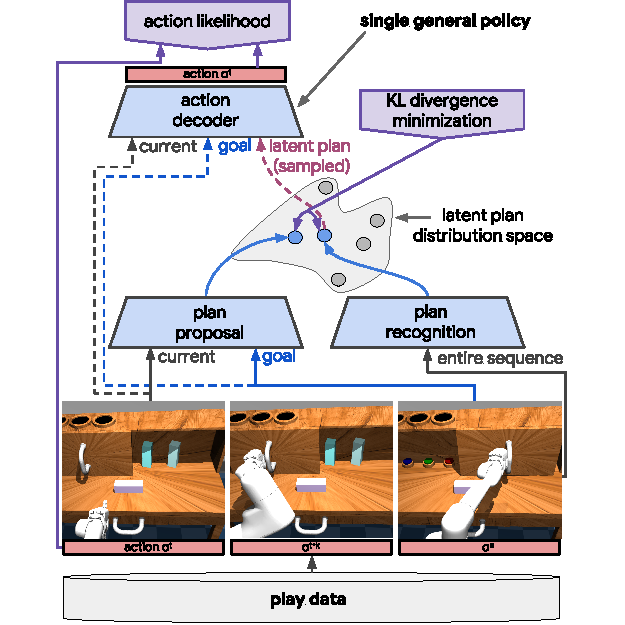
\includegraphics[height= 0.5\linewidth]{images/lmp_teaser5.pdf}
    \caption{Architecture used for the Learning from play method}
    \label{fig:LearningFromPlay}
\end{figure}


This approach has several key advantages:
\begin{itemize}
\item It is cheap: Large amounts of play data can be collected quickly since it doesn't require scene staging, task segmenting, or resetting to an initial state.
\item It is general: It encompasses both functional and non-functional behavior, relaxing the need for a predefined task distribution.
\item It is rich: Play naturally involves repeated, varied behavior, leading to high coverage of the possible interaction space. Additionally, the data is unlabeled, multimodal, and suboptimal.
\end{itemize}

\subsection{Resources}
There are many excellent resources on imitation learning and reinforcement learning. Much 
of the content presented here is based on Sergey Levine’s ''CS 285: Lecture 2 – Imitation 
Learning`` and ''Lecture 20 – Inverse Reinforcement Learning`` 
\cite{CS285,CS285LevineYoutube}. Additional resources that helped deepen my understanding 
of feature matching include ''Stanford CS234 – Reinforcement Learning | Offline RL 1 | 
2024, Lecture 8`` \cite{CS234Stanford}, and ''Maximum Entropy Inverse RL and Adversarial 
Imitation Learning`` by Katerina Fragkiadaki \cite{DeepRLandControl}. Another valuable 
reference on adversarial approaches is ''Deep RL Bootcamp – Lecture 10B: Inverse 
Reinforcement Learning`` \cite{DeepRlBootcamp}.

%    \item \href{https://www.youtube.com/watch?v=kGc8jOy5_zY}{CS 182: Lecture 14: Imitation Learning}

\section{Offline Reinforcement Learning}
Offline Reinforcement Learning is another paradigm of Reinforcement Learning. All previous 
methods we looked at are considered to be Online-RL methods. In Online-RL, the 
agent gathers data by directly interacting with the environment. It then uses this experience
immediately or via a replay buffer to update its policy, after which it has to interact with 
the environment again to collect more data.
\begin{figure}[H]
    \centering
    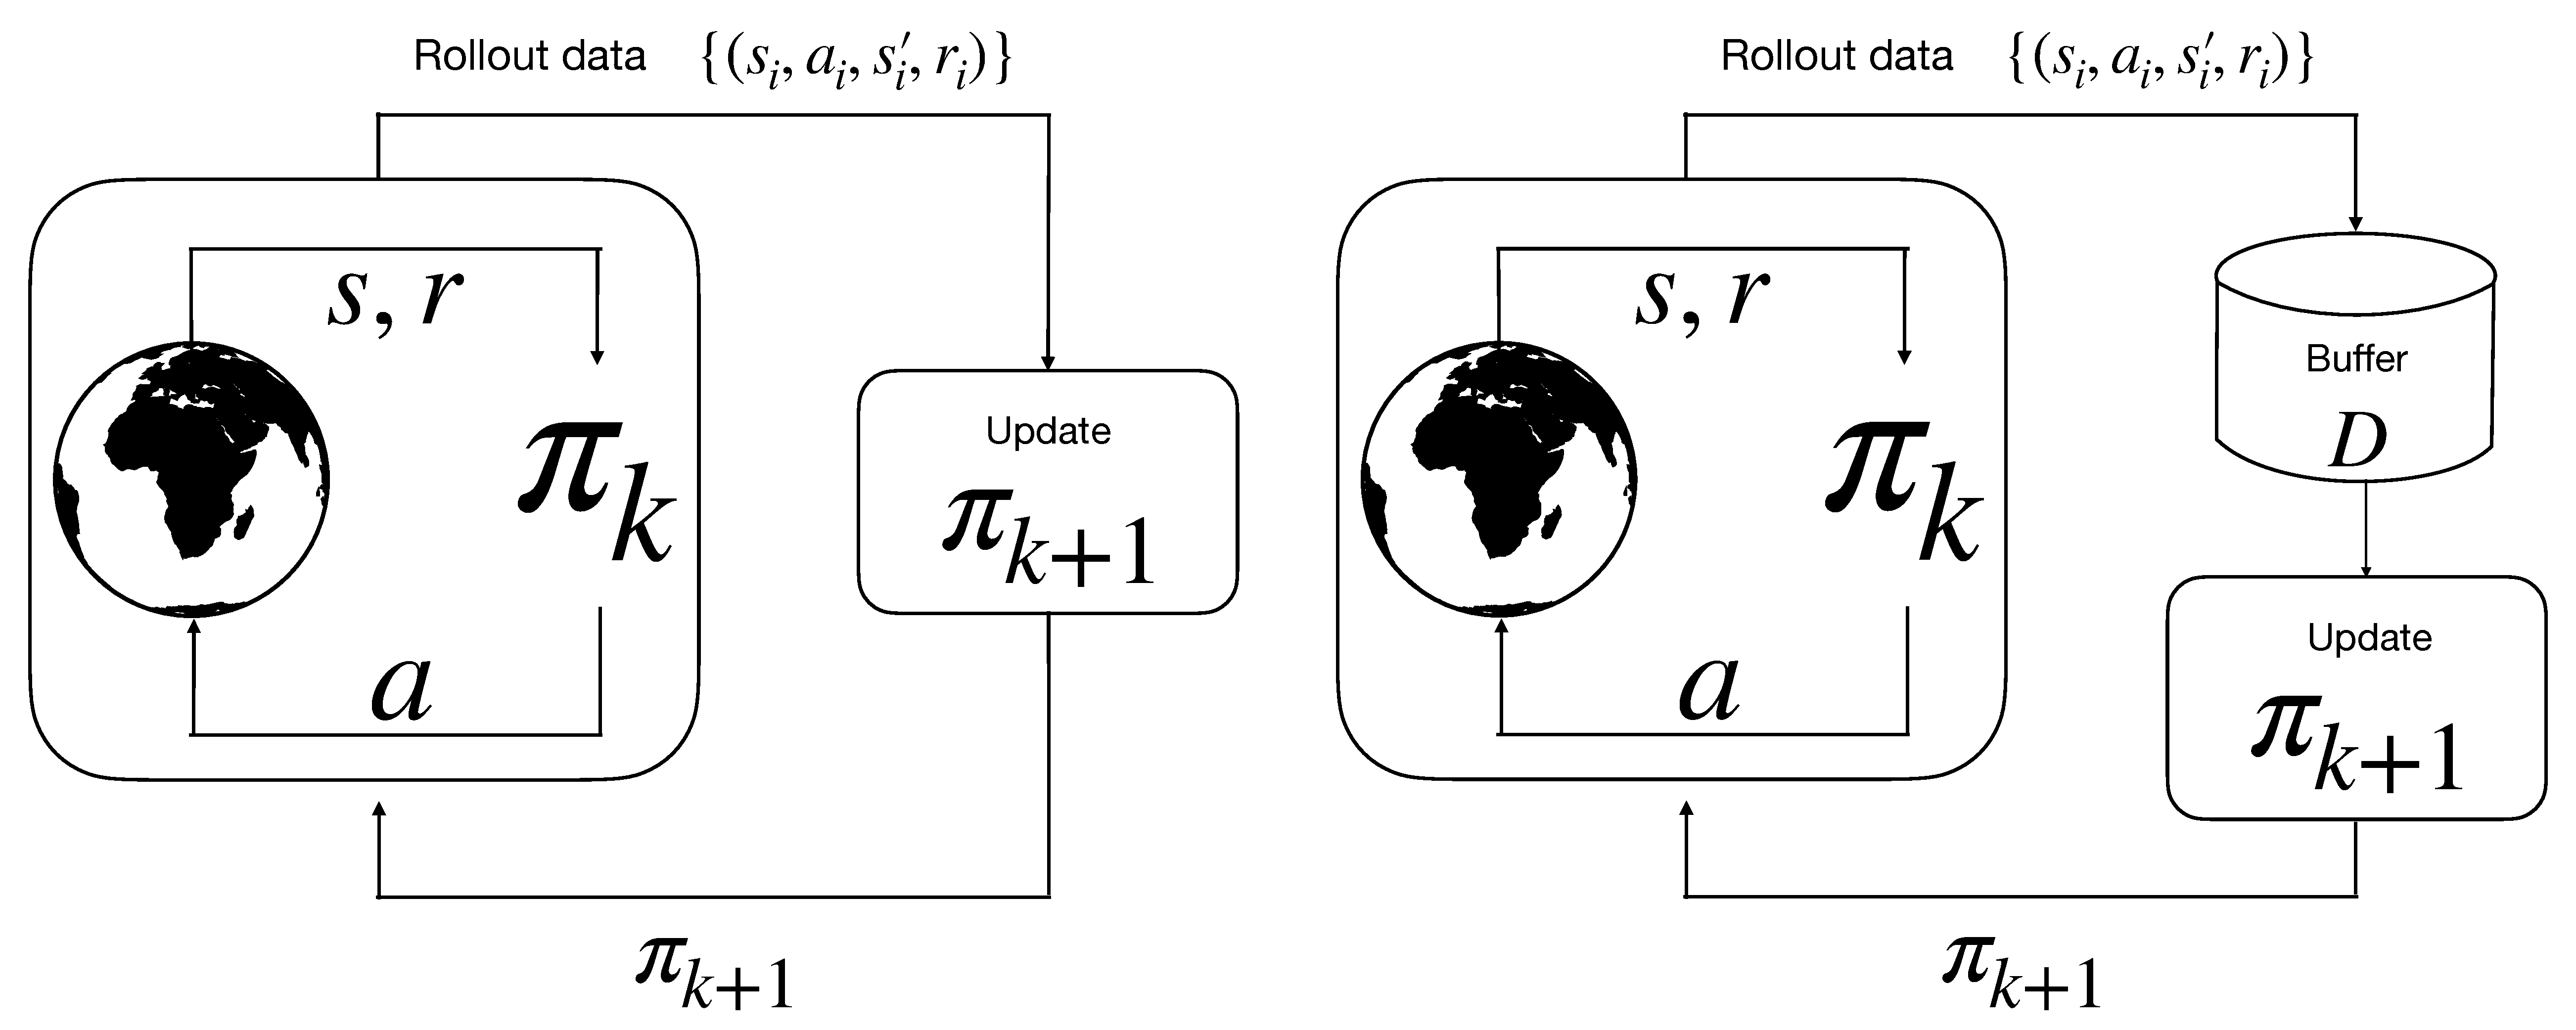
\includegraphics[width=0.8\linewidth]{images/off_vs_on_policy.pdf}
    \caption{Visualisation of online-RL as on-policy (left) and off-policy (right),inspired from 
    \cite{levine2020offlinereinforcementlearningtutorial}}
    \label{online_rl}
\end{figure}
Offline-RL is inspired by general deep learning. There we are just given a model and a 
large dataset to learn on. Throughout the training, the model does not interact in any way 
with anything outside the given data. But they are still able to generalise very well. In 
Offline-Rl, the agent only uses data collected from other agents and/or human 
demonstration to learn a policy, while not interacting with the environment once during 
training.
\vspace{-0.38cm}
\begin{figure} [H]
    \centering
    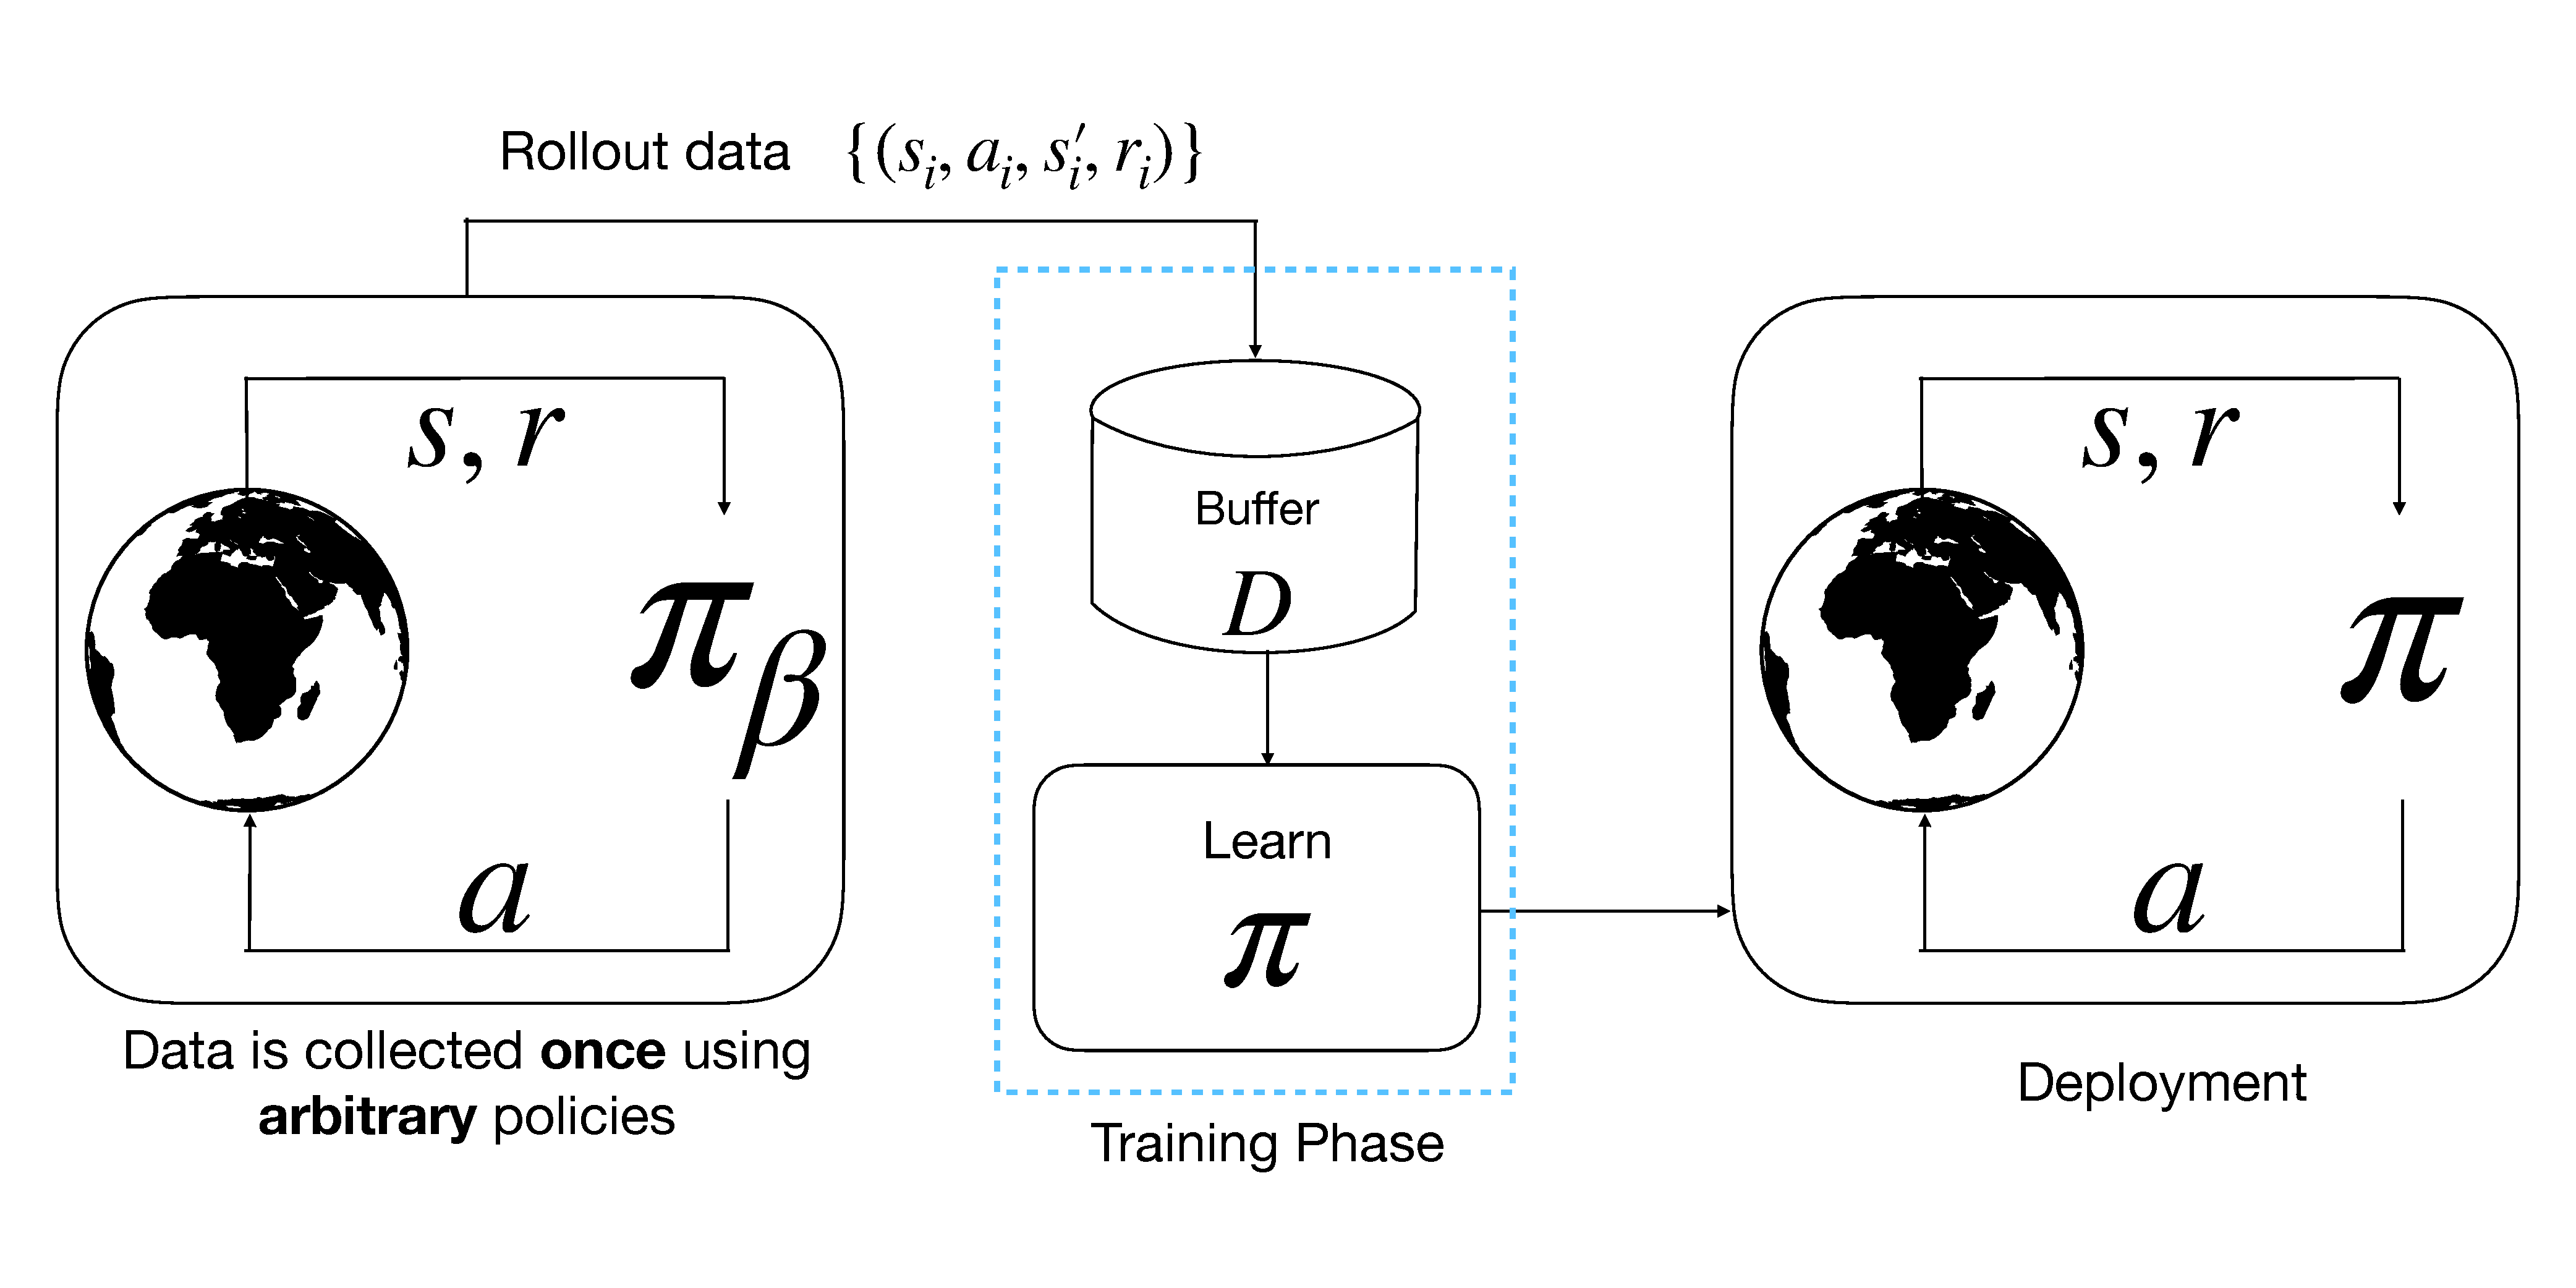
\includegraphics[width=0.8\linewidth]{images/offline_rl.pdf}
    \caption{Visualisation of Offline Reinforcement Learning, inspired from 
    \cite{levine2020offlinereinforcementlearningtutorial}}
    \label{offline_rl}
\end{figure}
In the following, we denote by $D$ the static dataset of transitions, defined as $D = \{(s_i, a_i, s_i', r_i)\}.$
The state-action tuples in this dataset are sampled such that the states $s$ are drawn from the stationary distribution 
$d^{\pi_\beta}(s)$ of a Markov chain (the distribution that remains unchanged over time under the dynamics induced by a 
policy). The actions $a$ are sampled from the behaviour policy $\pi_\beta(a \mid s)$, which is generally unknown.\newline
%The objective is then, as usual, to find the policy that maximises the expected sum of 
%discounted future rewards.
%$$\max\limits_\pi \underset{t=0}{\sum^T} \mathbb{E}_{s_t\sim d^\pi(s),a_t \sim \pi(a|s)}[\gamma^t r(s_t,a_t)]$$
The question that arises is whether we can hope to learn good policy without ever 
interacting with the environment. While we won’t formally prove it, the hope/claim is that
Offline RL can uncover the ''good stuff`` from a dataset that contains a mix of both good 
and bad behaviours. Importantly, the ''good stuff`` isn't limited to simply identifying the 
best trajectories in the dataset, but also includes the potential to learn policies that outperform
any single behaviour present in the data. This is based on the hope that Offline RL can generalize: 
that observing good behaviour in one context can inform good decisions in others. Ideally, the agent 
would be able to ''stitch together`` different pieces of good behaviour from across the dataset to construct 
an even better overall policy.
\begin{figure} [H]
    \centering
    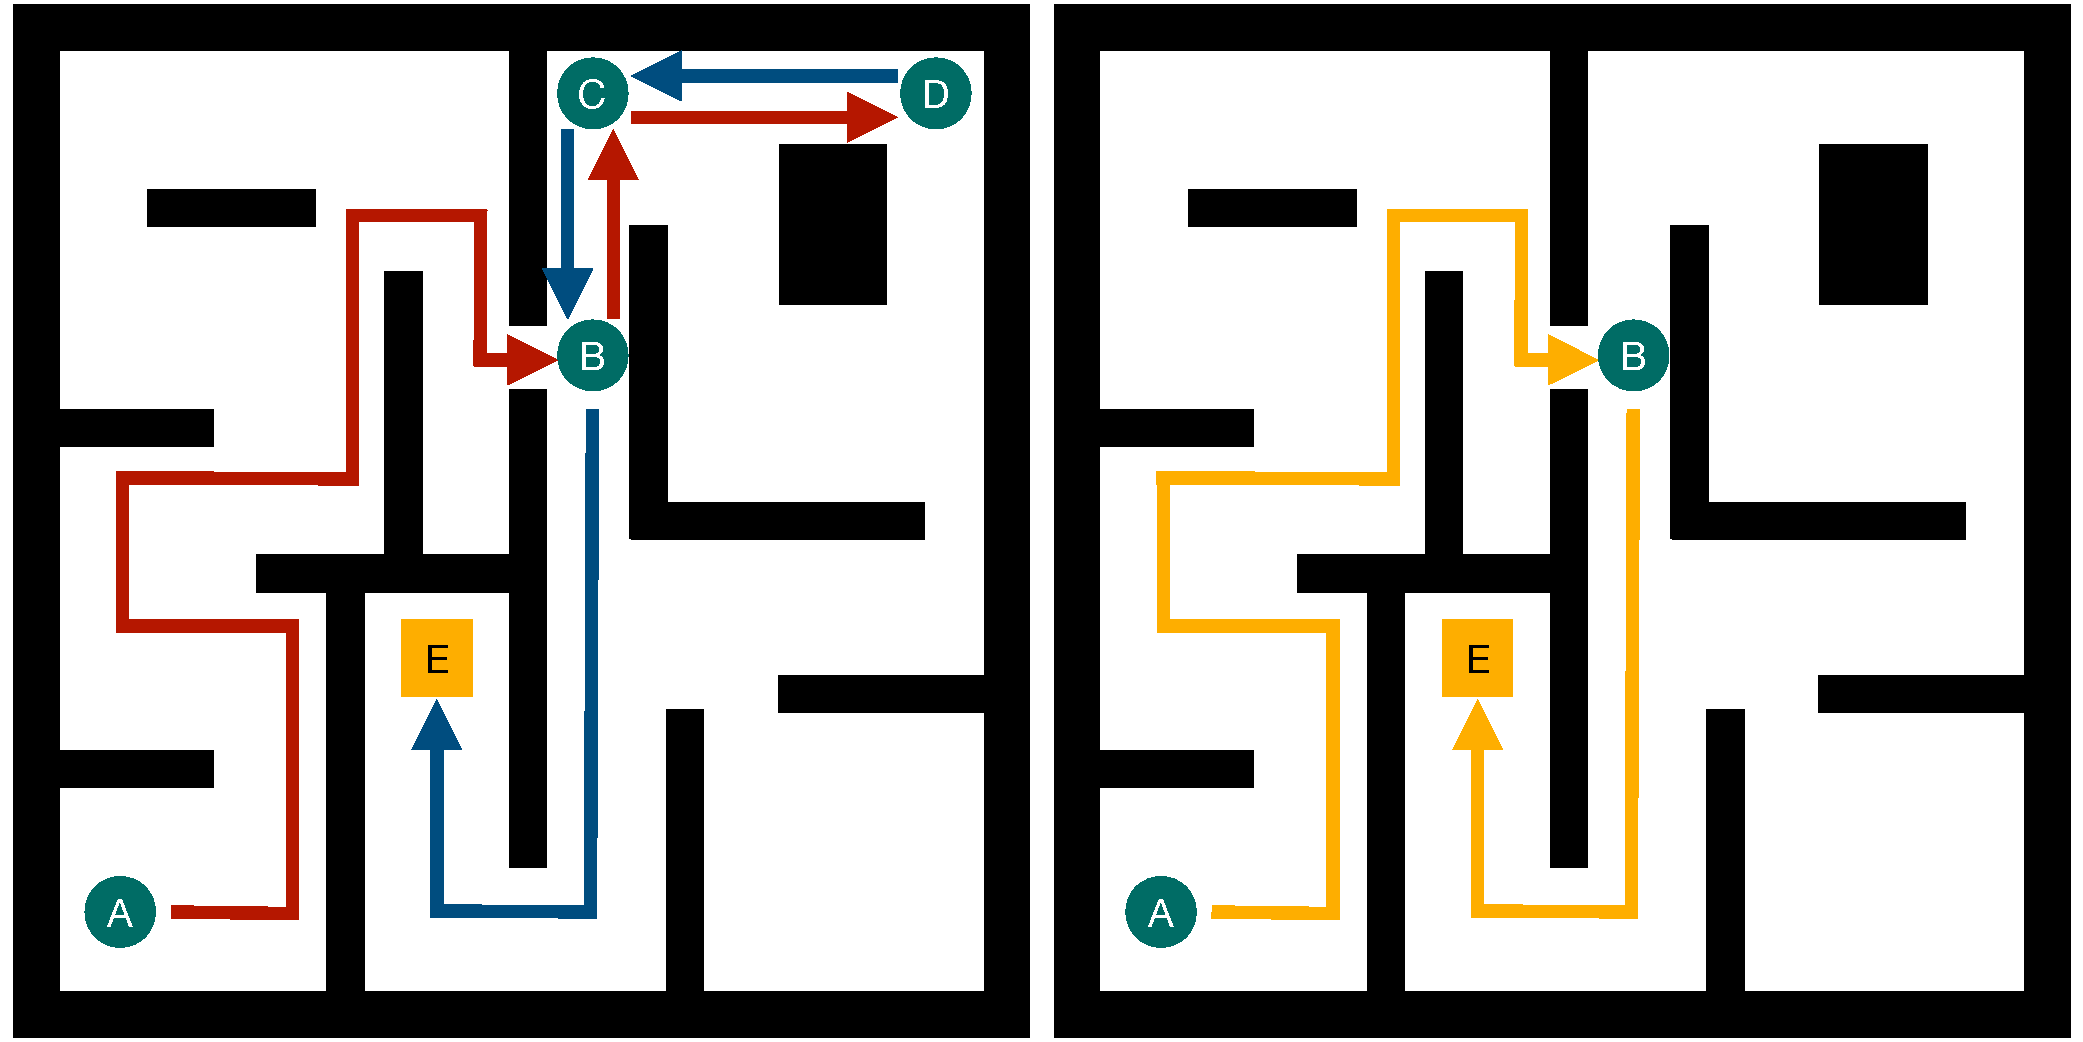
\includegraphics[width=0.6\linewidth]{images/maze_stitching.pdf}
    \caption{Visualization of the stitching process in Offline Reinforcement Learning. In the dataset, 
    we originally observe only partial trajectories—specifically, the segments from $ A \rightarrow D $
    and $ D \rightarrow E $ (as shown on the left). The stitching procedure combines these separate 
    trajectories to construct a new, potentially optimal path from $ A $ to the goal $ E $, 
    even though this complete path was never explicitly observed in the data. Inspired from 
    \cite{OfflineRL_Or_Imitation}}
    \label{offline_stitching}
\end{figure}
At first glance, Offline RL might seem quite similar to Imitation Learning (IL), since both involve learning 
from precollected datasets. This raises the question: can stitching also occur in IL methods?\newline
The key difference between the two settings lies in the availability of reward signals. Offline RL has access
to reward information, which enables the agent to distinguish between good and bad segments of behaviour. This
allows it to selectively stitch together high-quality parts of trajectories to construct better policies.\newline
In contrast, Imitation Learning typically does not have access to rewards. It relies solely on mimicking the observed 
behaviour, making it difficult to identify which parts of a trajectory are optimal or suboptimal. As a result, IL may end up 
stitching together poor behaviours or failing to prioritize the best ones. 

\subsection{Challenges in Offline-RL}
One problem that Offline-RL suffers from is overestimation. In 
\cite{kumar2019stabilizingoffpolicyqlearningbootstrapping} they did an experiment where 
they collected data from an agent that had been trained with some sort of SAC and had 
achieved reasonably good results. They used the data generated by this agent to fill a 
replay buffer which then was used for doing Offline-RL on the same task. As you can see in 
figure \ref{off_rl_overestimation}, the actual return is really bad while the Q values are 
very high. So the Offline-RL agent is certain that it actions will lead to high reward but 
in reality the opposite is true. In the following, we will explore from where this problem arises
and discuss potential strategies to mitigate it.
\begin{figure}[H]
    \centering
    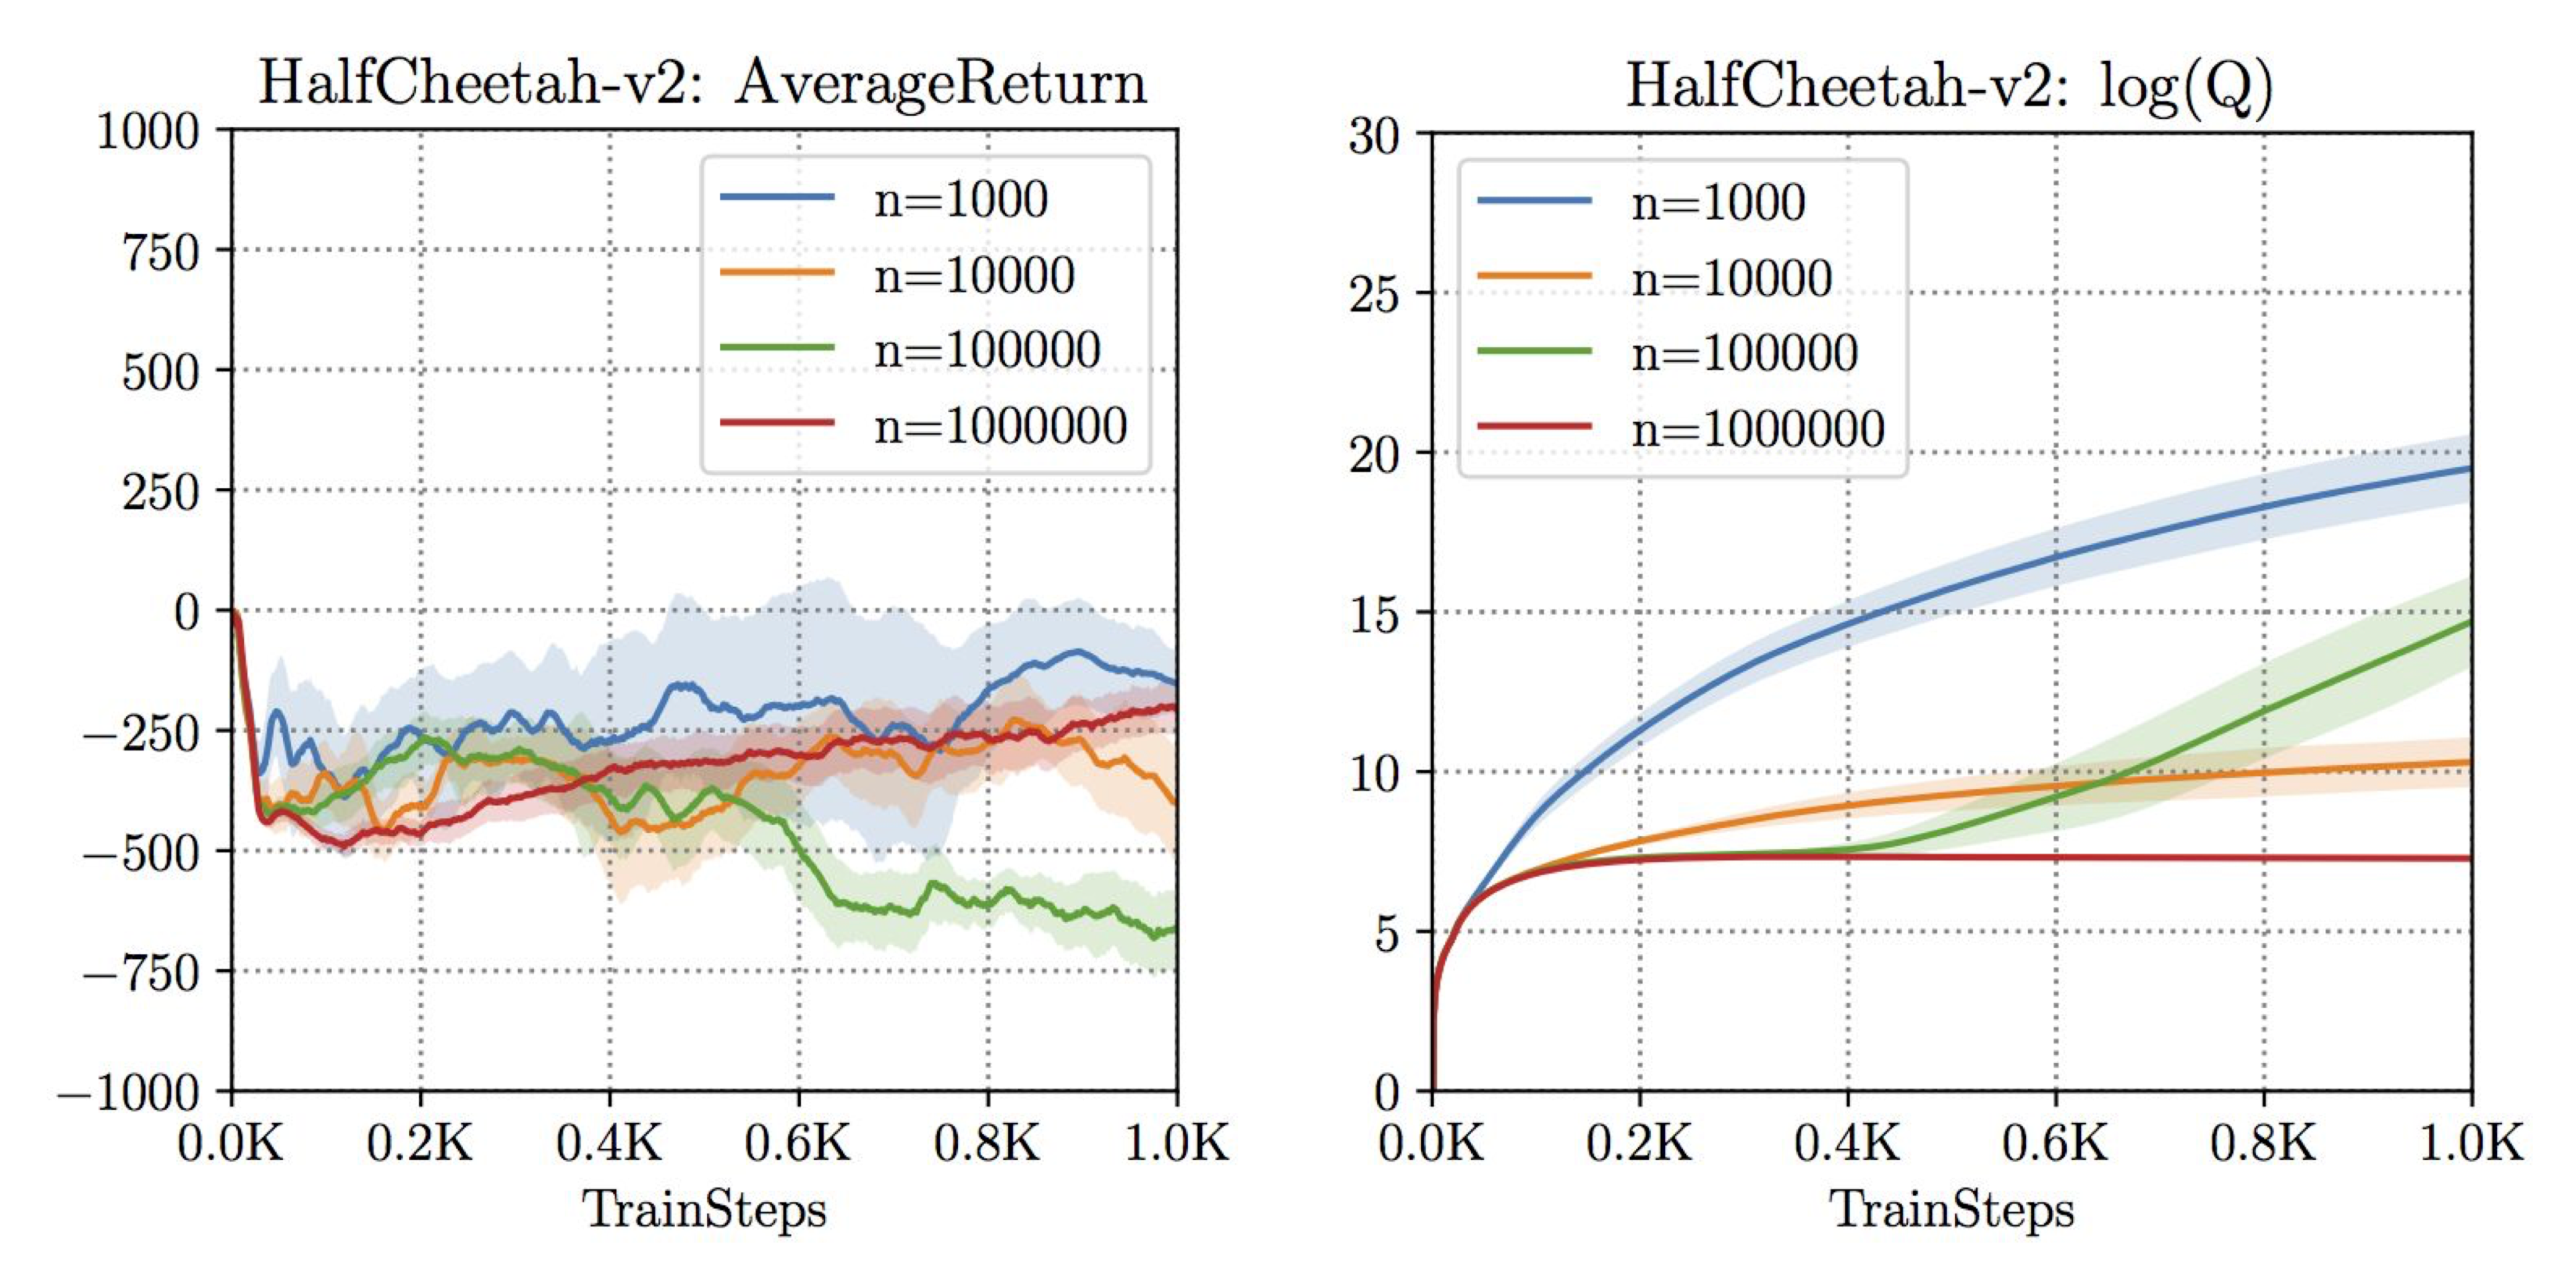
\includegraphics[width=0.72\linewidth]{images/off_rl_problem.png}
    \caption{Performance of SAC on HalfCheetah task with off-policy expert data 
    w.r.t. number of training samples (n), from \cite{kumar2019stabilizingoffpolicyqlearningbootstrapping}}
    \label{off_rl_overestimation}
\end{figure}

\subsubsection{Intuitive Explanation}
The intuitive way to understand the challenge of Offline RL is through counterfactuals. Counterfactuals 
are if statements where the if part is not realised. For example, you are on your way home 
and arrive at a fork in the road where you can either go left or right. Both ways lead to 
your home. So you decide to go left, thinking it would be faster, only to learn that you will
get stuck in traffic and arrive home late. The counterfactual is now ''I should have went right``,
or in other words, ''If I had went right, it would have been better``, even though you do not know
the outcome of going right because you never took it. The core problem is that you are making 
assumptions about the outcomes of actions based solely on the outcomes of the actions you have 
taken without ever observing what would have happened had you chosen differently.\newline 
In Offline RL, such reasoning is necessary. Because for Offline RL to produce policies that outperform
the behaviour seen in the dataset it must consider actions beyond those explicitly observed in the data.
So when updating/executing the policy/Q-values, we typically compare all possible actions in a given state to 
identify the best one. This inherently involves counterfactual reasoning. Because the action we believe 
to be optimal, because it has the highest predicted Q-value, might never been actually observed in the dataset.
If we select it anyway, we are relying entirely on predictions, with no evidence to back them up and so doing
counterfactual reasoning.\newline 
However, counterfactual reasoning in Offline RL brings about a deeper, more subtle problem: distributional shift which 
we already saw when we looked at Imitation Learning and Model-Based-Reinforcement-Learning. Offline RL inherently involves 
making predictions about what would happen under a different policy than the one that generated the data. So it seeks 
to learn a new policy that deviates from the behavior policy ideally to achieve better performance which naturally leads to a 
shift in the distribution of visited states and actions. This shift manifests in two key ways. First, the learned policy may 
visit parts of the state space that were rarely or never seen in the dataset. Second, even in familiar states, it may prefer 
different actions than those taken by the behavior policy (see above explanation). In both cases whether policies, value 
functions, or models—are forced to make predictions under conditions different from those they were 
trained on (distributional shift).\newline
Unlike online RL methods, which can try the action and learn from its outcome, offline methods do not have this luxury. As a 
result, Offline RL must find ways to handle uncertainty around unseen actions (out-of-distribution (OOD)) typically by 
regularizing, constraining, or penalizing those actions during learning.

\subsubsection{Mathematical Explanation}
We now turn to the mathematical explanation of the problem. In general machine learning, our objective is 
typically framed as risk minimization:
 $$\theta \gets \argmin\limits_\theta \mathbb{E}_{x\sim p(x),y \sim p(y|x)}[(f_\theta(x)-y)^2]$$
After training, we might ask: Given a new input $x^*$, is the model's prediction $f_\theta(x^*)$ likely to be accurate?
In expectation, the error is low but only if $x^* \sim p(x)$  so if it comes from the same distribution as the training data. 
If $x^*$ is drawn from a different distribution, this guarantee no longer holds.\newline 
Moreover, if we move away from evaluating under expectation and consider individual inputs, we lose even more certainty. We 
can not guarantee low error, even if $x^*$ was from the training set. This can be easily exploited if we choose 
$x^* \gets \argmax\limits_x f_\theta(x)$.\newline 
In methods like Q-Leaning- or Actor-Critic-methods, we compute the target values $y$ under some policy $\pi_\text{new}$ and try to regress them onto the Q-values
\begin{gather*}
    Q^{k+1}= \argmin\limits_Q \mathbb{E}_{s,a,s' \sim D \sim {\color{cyan}\pi_\beta}}[(Q(s,a)-y(s,a,s'))^2] \\
    \text{with }y(s,a,s') = r(s,a)+\mathbb{E}_{a' \sim {\color{red}\pi^k}}[Q^k(s',a')] \qquad (\text{see footnote \footnotemark})
\end{gather*}
Similar to above, we expect the Q values to be accurate if $\pi^k(a|s) = \pi_\beta(a|s)$. But the whole point of offline-RL is that $\pi^k \gg \pi_\beta$, and to make matters worse, in most methods we choose 
 $$\pi^{k+1} = \argmax\limits_\pi \mathbb{E}_{s\sim D,a\sim \pi^k(a|s)}[Q^{k+1}(s,a)]$$ so we are explicitly trying to find actions that produce high Q values.
 \footnotetext{
$y = r(s,a)+\mathbb{E}_{a' \sim {\pi^k}}[Q^k(s',a')]$ may seem unfamiliar at first, as we initially defined the targets as 
$r(s,a) + \gamma \max\limits_{a'} Q^k(s', a').$
However, we can rewrite this expression as
$r(s,a) + \gamma Q^k\left(s', \arg\max_{a'} Q^k(s', a')\right),$
which, using the relationship in Equation~\eqref{eq:v_to_q}, leads us back to the same formulation.
 }


 \subsection{Approaches to Offline-RL}
%There are several ways to deal with this overestimation problem in offline-RL. The oldest, 
%but no longer used, methods are to use important sampling or linear fitted value 
%functions, while current methods use policy constraints, which we will look at 
%next.\newline
The most common approach for addressing the distributional shift problem in Offline-RL is to impose constraints on how much 
the learned policy is allowed to deviate from the behaviour policy, leading to an optimization objective of the form:
$$\pi_\text{new} = \argmax\limits_\pi \mathbb{E}_{a\sim \pi(a|s)}[Q(s,a)] \quad 
\text{s.t.} \quad \text{Diff}(\pi||\pi_\beta)\leq \epsilon$$ 
This approach comes with two key challenges. First, the constraint may not be pessimistic enough. Even if two policies are 
close in terms of a divergence metric (like KL), they can still differ significantly at specific states. This means the 
learned policy might take actions in certain states where the Q-values are poorly estimated, leading to unreliable 
behaviour.\newline 
Second, if the constraint is too pessimistic, it can prevent the learned policy from meaningfully improving over the behaviour 
policy. In such cases, the policy is forced to stay so close to $\pi_\beta$ that it cannot explore better actions, limiting 
its potential to exceed the performance of the dataset policy.\newline 
For simplicity, in the following we always use the KL as the distance measure for the 
constraint, but it also can be any other measure for probabilities.\newline
To better understand the second challenge, consider Figure \ref{out_of_support}.  We are given the behaviour policy $\pi_\beta$ (blue) for a single 
state. The blue dots represent samples from our data set where y values correspond to q values. The q-function fitted to 
these samples is given by the orange function. If we now train a policy that maximises the q values but also satisfies the 
constraint, we get $\pi_\text{KL}$ (red). You can see that this policy does not only focus on the actions with the highest 
q-values, but also assigns non-negligible probabilities to actions with low q-values. The reason for this is that the KL 
constraint forces it to be something like $\pi_\beta$. Intuitively, we would want something like $\pi_\text{support}$ (green),
but that violates the constraint because the variance is so far off.\newline 
What comes closer to what we want but is more difficult to implement are support constraints 
$$\pi(a|s) > 0 \iff \pi_\beta(a|s) \geq \epsilon $$
\begin{figure}[H]
    \centering
    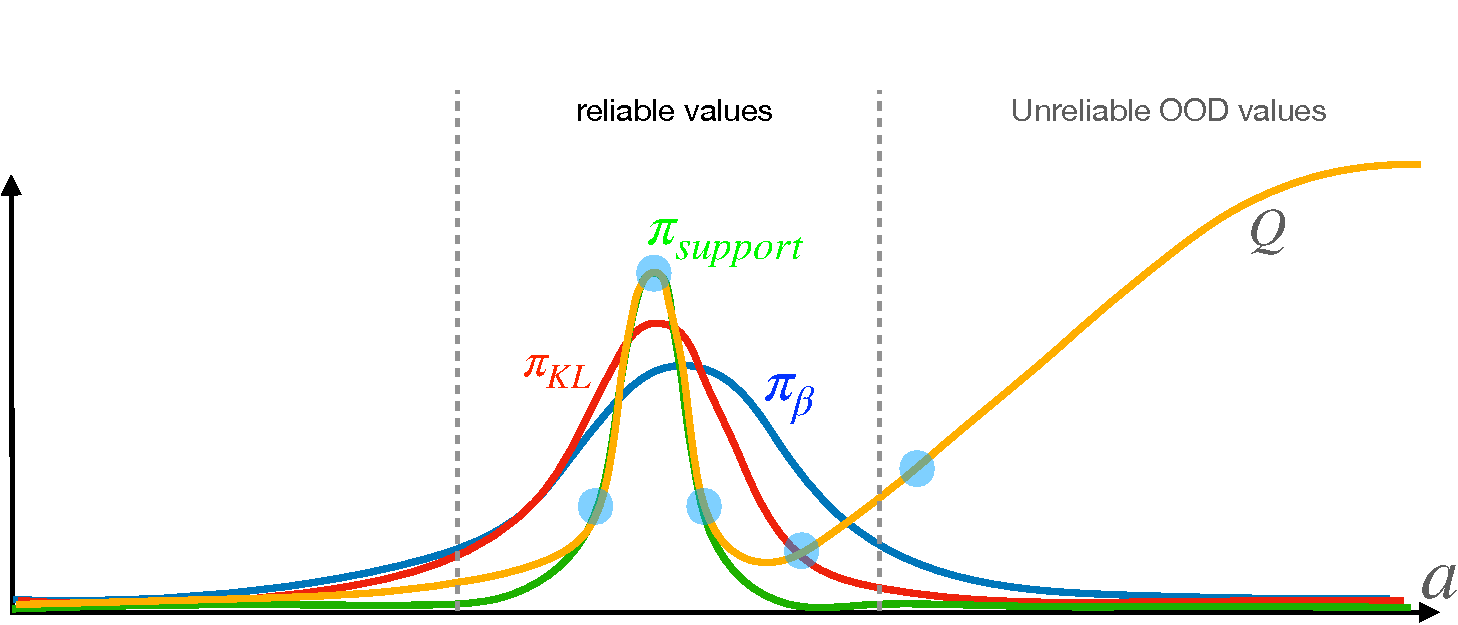
\includegraphics[width=0.8\linewidth]{images/explicit_offline_rl.pdf}
    \caption{Visualization of explicit policy constraints using KL divergence. Inspired by CS 285: Lecture 16 \cite{CS285,CS285LevineYoutube}.}
    \label{out_of_support}
\end{figure}
\subsubsection{Explicit Policy Constraints}
One common approach to incorporating policy constraints in Offline RL is to solve the constrained optimization problem using 
the method of Lagrange multipliers. This leads to the following objective:
\begin{align*}
     \pi_\text{new}(a|s) &= \argmax\limits_\pi \mathbb{E}_{a\sim \pi(a|s)}[Q(s,a)] - \lambda \text{KL}(\pi||\pi_\beta) \\
     %&= \argmax\limits_\pi \mathbb{E}_{a\sim \pi(a|s)}[Q(s,a)] - \lambda \mathbb{E}_{\pi}[\log{\pi(a|s)}-\log{\pi_\beta(a|s)}] \\
     %&= \argmax\limits_\pi \mathbb{E}_{a\sim \pi(a|s)}[Q(s,a)] - \lambda \left(-H(\pi(a|s))-\mathbb{E}_\pi(\log{\pi_\beta(a|s)})\right) \\
      &= \argmax\limits_\pi \mathbb{E}_{a\sim \pi(a|s)}[Q(s,a)+\lambda \log{\pi_\beta(a|s)}] + \lambda H(\pi(a|s)) 
\end{align*}
Here, the Lagrangian multiplier $\lambda$ can either be computed via dual optimization or treated as a hyperparameter. 
However, since we're not solving for the policy in closed form, we simply optimize the objective directly. An alternative idea 
is to incorporate the constraint directly into the reward function:
$$r_\text{diff}(s,a) =r(s,a)- \text{KL}(\pi||\pi_\beta)$$
While this explicit approaches using KL constraints are simple to implement, they rely on access to the behaviour policy $\pi_\beta$ which is often unknown in practice. One idea is to learn $\pi_\beta(a|s)$ from the data via a model. Another idea is to cleverly implement the constraint that we only need access to the samples, not the probabilities which we will looking at in the following.

\subsubsection{Implicit Policy Constraints}
When we once again express the constrained objective using the Lagrangian and this time solve for the optimal 
policy in closed form, we obtain:
$$\pi^*(a|s) = \frac{1}{Z(s)}\pi_\beta(a|s)\exp{\frac{A^{\pi_\text{old}}(s,a)}{\lambda}}$$ 
Here $Z(s)$ is the normalizing constant to ensure the result is a valid probability distribution, and $\lambda$ is the 
Lagrangian multiplier. This optimal policy can now be approximated via maximum likelihood estimation, yielding the 
following objective:
$$\pi_\text{new}(a|s)= \argmax\limits_\pi \mathbb{E}_{(s,a)\sim \pi_\beta}\left[\frac{1}{Z(s)}\log{(\pi(a|s))}\exp{\frac{A^{\pi_\text{old}}(s,a)}{\lambda}}\right]$$
Notably, this formulation does not require explicit evaluation of $\pi_\beta$ only to draw samples from it.
However, it still suffers from the problem of out-of-distribution actions, as computing advantages using Q-values requires 
querying actions that lie outside the behaviour policy’s distribution. In the following 
we will look at methods which try to completely avoid outer distribution action in the Q-update and so
preventing the overestimation issue.

\subsubsection{Implicit Q-Learning}
The update rule for the Q-function can be expressed using the value function as follows:
$$Q(s,a) \gets r(s,a)+\gamma \mathbb{E}_{a'\sim \pi_\text{new}}
[Q(s',a')]\overset{eq. \eqref{eq:v_to_q}}{=} r(s,a)+\gamma V^{\pi_\text{new}}(s')$$ 
We assume that $V(s') $ is represented by a neural network. When we regress $ V $ onto $ Q(s, a) $ 
using mean squared error (MSE) as we've done previously we end up approximating the Q-function 
corresponding to $ \pi_\beta $, since our dataset is generated by $ \pi_\beta $. Thus, we are effectively learning 
$ Q_{\pi_\beta} $ rather than $ Q_{\pi_\text{new}} $.\newline
An important observation is that, in large or continuous datasets, individual states are often visited only once, with 
typically a single action taken per state. However, nearby similar states may be visited with different actions. In practice, 
the policy generalizes across such states, meaning the targets are not fixed values but rather form a distribution (see 
Figure~\ref{v_value_dist}).
\begin{figure}[H]
    \centering
    \resizebox{!}{5cm}{
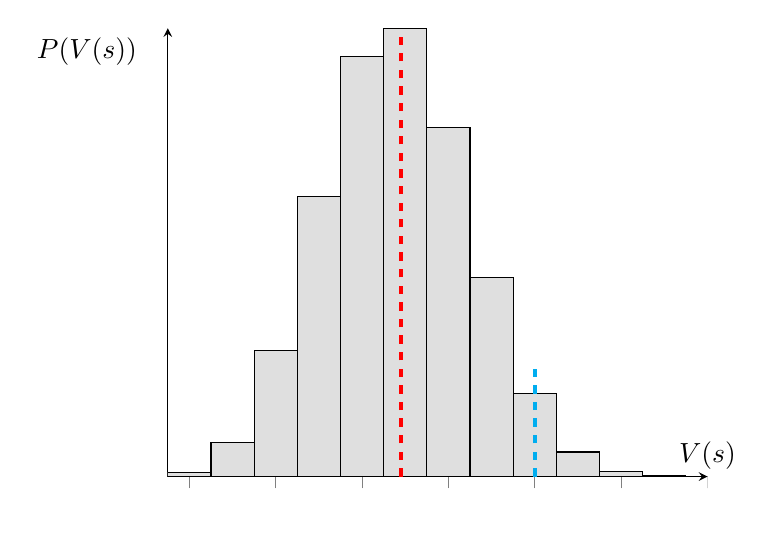
\begin{tikzpicture}[
    declare function={binom(\k,\n,\p)=\n!/(\k!*(\n-\k)!)*\p^\k*(1-\p)^(\n-\k);}
]
\begin{axis}[ymin=0, xmin=-0.5,axis lines=left,xlabel={$V(s)$}, xticklabels={},yticklabels={,,} ,ylabel={$P(V(s))$}, x label style={at={(axis description cs:1,0.1)},anchor=north},
    y label style={at={(axis description cs:-0.15,1)},rotate = -90, anchor=north}, ,
    samples at={0,...,12},
    yticklabel style={
        /pgf/number format/fixed,
        /pgf/number format/fixed zerofill,
        /pgf/number format/precision=2
    },
    ybar=0pt, bar width=1, bar shift=0pt
]
\addplot [fill=gray!25,] {binom(x,12,0.4)}; 
\addplot [fill=gray!25, samples at={0,...,4}] {binom(x,12,0.4)};
\addplot [fill=gray!25, samples at={7}] {binom(x,12,0.4)};
\def\ymin{\pgfkeysvalueof{/pgfplots/ymin}}
  \def\ymax{\pgfkeysvalueof{/pgfplots/ymax}}
  \draw[ultra thick, dashed,color = cyan] 
    ($(axis cs:7, \ymin)!.5!(axis cs:9, \ymin)$) -- 
    ($(axis cs:7, 0.25*\ymax)!.5!(axis cs:9, 0.25*\ymax)$)
  ;
    \draw[ultra thick, dashed,color = red]
    ($(axis cs:4, \ymin)!.9!(axis cs:5, \ymin)$) --
    ($(axis cs:4, 1.2*\ymax)!.9!(axis cs:5, 1.2*\ymax)$) node[] {Your Text Here}
  ;

\end{axis}
\end{tikzpicture}}
\caption{Probability distribution of the value function for a given state}
\label{v_value_dist}
\end{figure}
When performing MSE regression, the model tends to predict the mean of the value distribution represented 
by the red dashed line. However, what we actually want is to focus on the upper quantile, where the value
under the optimal policy is supported by the data (illustrated by the cyan dashed line).  
To achieve this Implicit-Q-Learning \cite{kostrikov2021offlinereinforcementlearningimplicit} uses the expectile 
regression loss, defined as:
$$L_\text{expectile}(x) = 
\begin{cases}
(1-\mu)x^2,\quad \text{if } x> 0\\ \mu x^2\qquad\qquad \text{else} 
\end{cases}$$ 
The purpose of this loss function is to penalize negative errors more heavily than 
positive ones, encouraging predictions of higher values. At first glance, this may appear 
to contradict the goal of avoiding overestimation. However, overestimation does not occur 
in this case because all the actions we take are drawn from within our dataset, ensuring 
that no out-of-distribution (OOD) actions are involved. As a result, we can update our Q-
functions without the risk of out-of-distribution actions.\newline
What can be shown is that this implicit Q-learning corresponds to support constraints:
$$V(s) \gets \max_{a \in \Omega(s)} Q(s,a) \quad \text{with} \quad \Omega(s) = \{a:\pi_\beta(a|s)\geq \epsilon\}$$

\subsubsection{Conservative Q-Learning}
Conservative Q-Learning (CQL) \cite{kumar2020conservativeqlearningofflinereinforcement} aims to mitigate overestimation in 
offline reinforcement learning by explicitly penalizing large 
Q-values, especially for out-of-distribution (OOD) actions. The core idea is to modify the Q-learning objective as follows:
$$Q^\pi = \argmin\limits_Q \mathbb{E}_{(s,a,s')\sim D}\left[\left(Q(s,a)-(r(s,a)+\mathbb{E}_\pi[Q(s',a')])\right)^2\right] + \max_\mu \alpha \mathbb{E}_{s\sim D, a\sim \mu(a|s)}[Q(s,a)] $$ 
Here, the second term penalizes large Q-values under some auxiliary policy $\mu$, encouraging conservatism by lowering Q-
values for actions not present in the dataset $D$.\newline
However, this approach can become overly pessimistic-reducing all Q-values, including those that are not overestimated. To 
address this, a corrective term is introduced that subtracts the expected Q-value over the dataset distribution. The full CQL 
loss becomes:
\begin{align*}
    Q^\pi =\argmin\limits_Q \mathbb{E}_{(s,a,s')\sim D}\left[\left(Q(s,a)-(r(s,a)+\mathbb{E}_\pi[Q(s',a')])\right)^2\right] &+ \underbrace{\max_\mu \alpha \mathbb{E}_{s\sim D, a\sim \mu(a|s)}[Q(s,a)]}_{\text{punish big Q-values}} \\&- \underbrace{\alpha \mathbb{E}_{(s,a)\sim D}[Q(s,a)]}_{\text{unless they from dataset}}
\end{align*}

%Thus, Conservative Q-Learning follows the following loop:
%\begin{enumerate}
%    \item update $Q^\pi$ w.r.t. $L_{CQL}$ using dataset $D$
%    \item update policy $\pi$
%\end{enumerate}

\subsection{Resources}
This section is largely based on Sergey Levine’s CS 285 ''Lecture 15 – Offline Reinforcement Learning`` and ''Lecture 16 – Offline Reinforcement Learning 2``\cite{CS285,CS285LevineYoutube}. For a more in-depth comparison between Offline Reinforcement 
Learning and Imitation Learning, see \cite{kumar2022preferofflinereinforcementlearning}.

\section{Transformers in Reinforcement Learning}
Transformers, originally developed for sequence modeling in natural language processing, have attracted growing interest in 
reinforcement learning (RL) due to their ability to capture long-range dependencies and handle complex sequential data. In the 
following sections, we will first explore the core mechanisms of the transformer architecture, and then discuss how the standard 
transformer is adapted for use in RL. However, we will not delve deeply into specific RL papers that apply transformers.
At a high level, the process of how an input is processed by a transformer can be broken down into a series of steps: \newline
\vspace{-0.8cm}
\begin{wrapfigure}[16]{r}{5.5cm}
    \caption{Transformer architecture from \cite{vaswani2023attentionneed}}
    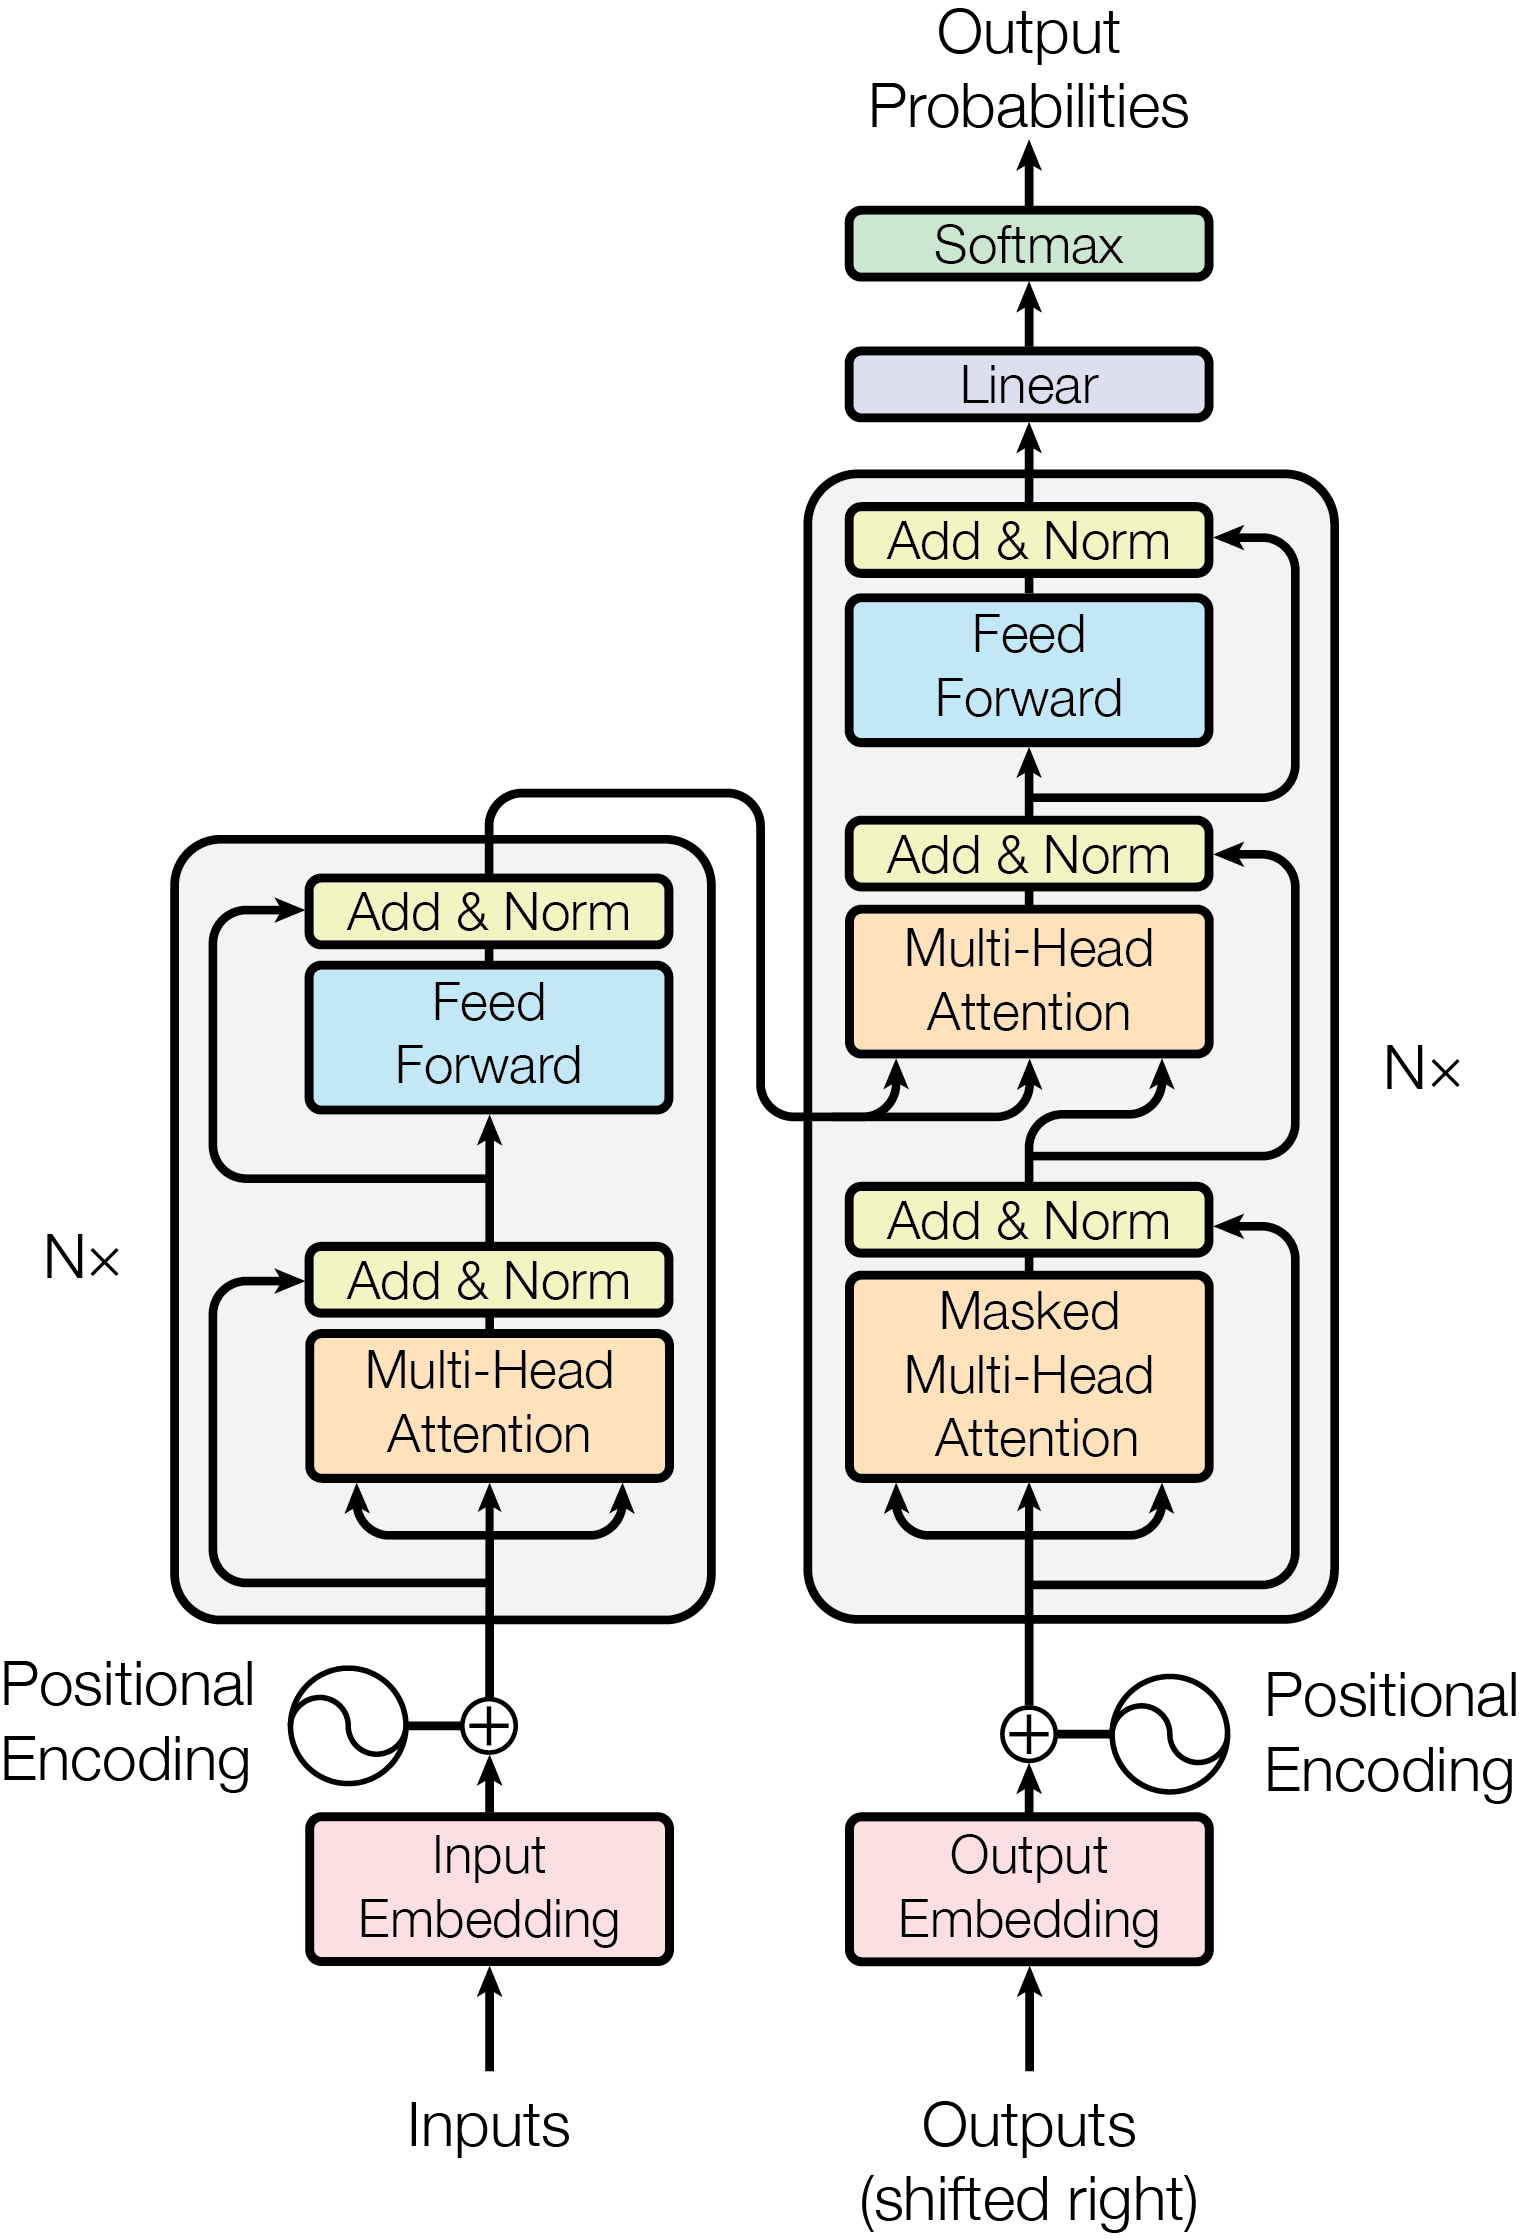
\includegraphics[height=10cm]{images/ModalNet-21.png}
    \label{transformer}
\end{wrapfigure}
\begin{enumerate}
\item \textbf{Input Embedding:} Converts input tokens or data into dense vector representations. In NLP, this applies to 
words/tokens; in RL or vision tasks, states or images are embedded.

\item \textbf{Positional Encoding:} Adds position information to embeddings, allowing the transformer to capture sequence 
order, which it doesn't handle inherently.

\item \textbf{Self-Attention Mechanism:} Enables each token to attend to all others using learned query, key, and value 
vectors. Attention scores—based on query-key similarity—determine how much focus each token gives to others, producing a 
weighted sum of values.

\item \textbf{Feedforward Network:} Applies a fully connected neural network to each position independently for further 
transformation.

\item \textbf{Residuals \& Layer Norm:} Residual connections and layer normalization follow attention and feedforward layers 
to stabilize training and preserve information.

\item \textbf{Stacked Layers:} Multiple layers refine the representations, allowing deeper abstraction and more complex 
understanding.

\item \textbf{Output:} Final outputs vary by task—e.g., softmax classification in NLP or decision-making in RL.
\end{enumerate}
%\begin{enumerate}
%\item  Input Embedding: The input is first converted into embeddings. For NLP tasks, this might involve 
%converting words or tokens into dense vector representations. In other applications, such as RL or image 
%processing, this could involve encoding states or images into suitable embeddings.

%\item Positional Encoding: Since transformers don't inherently capture the order of the input sequence (like 
%RNNs or LSTMs), positional encodings are added to the embeddings to inject information about the position of 
%each element in the sequence. These encodings are usually vectors that represent the position of tokens in 
%the sequence.

%\item Self-Attention Mechanism: The key feature of the transformer is the self-attention mechanism. For each 
%element in the sequence (e.g., word or state), the model computes attention scores with respect to all other 
%elements in the sequence. This allows each token to "attend" to every other token, enabling the model to 
%capture relationships and dependencies across the entire sequence.

%\item Attention Scores and Weighted Sum: The attention mechanism calculates a weighted sum of all input 
%embeddings based on how much focus each token should have on others. This is done using three learned vectors 
%per token: queries, keys, and values. The attention score between two tokens is calculated as the similarity 
%between their query and key vectors.

%\item Feedforward Neural Networks: After the self-attention step, each token's representation is passed 
%through a feedforward neural network. This helps further process the information and allow for more complex 
%transformations of the input sequence.

%\item Residual Connections and Layer Normalization: To prevent the model from losing information through deep 
%layers, transformers use residual connections around both the attention and feedforward layers, followed by 
%layer normalization. This helps stabilize training.

%\item Multiple Layers: The transformer consists of multiple layers of attention and feedforward networks. 
%Each layer refines the input, allowing the model to capture increasingly complex relationships between tokens 
%or elements in the sequence.

%\item Output: The final output of the transformer can be processed in various ways, depending on the task. 
%For instance, in NLP tasks, the output might be passed through a softmax layer for classification, or in RL, 
%it might inform the next action or state prediction.

%\end{enumerate}
\noindent
In the following, we will take a closer look at the individual steps, primarily focusing on 
language processing. However, it's important to note that transformers are not limited to 
language—they can also process other types of inputs, such as images. We focus on language 
processing here simply because it's a clear and intuitive way to understand the core steps 
of how transformers work.

\subsection{Embedding}
The first stage in training a transformer model involves converting raw input into vector representations—a process known as 
input embedding. A basic approach to representing words is one-hot encoding, where each word is assigned a binary vector the 
size of the vocabulary, with a single 1 indicating the presence of that word and 0s elsewhere. Although simple, this method 
has significant drawbacks: the vectors are high-dimensional, sparse, and fail to capture any semantic relationships between 
words.\newline 
To address these limitations, learned word embeddings are used. These are dense, low-dimensional vectors trained to capture 
semantic meaning, typically using unsupervised learning techniques. Words with similar meanings are mapped to similar vector 
representations. For example, the vectors for “queen” and “woman” will lie close in the embedding space due to shared 
contextual usage. Embeddings can also reflect relationships, such as vector arithmetic:
$$\text{vector(queen)}\approx \text{vector(king)}+\text{vector(woman)}-\text{vector(man)} $$
\begin{figure}[H]
    \centering
    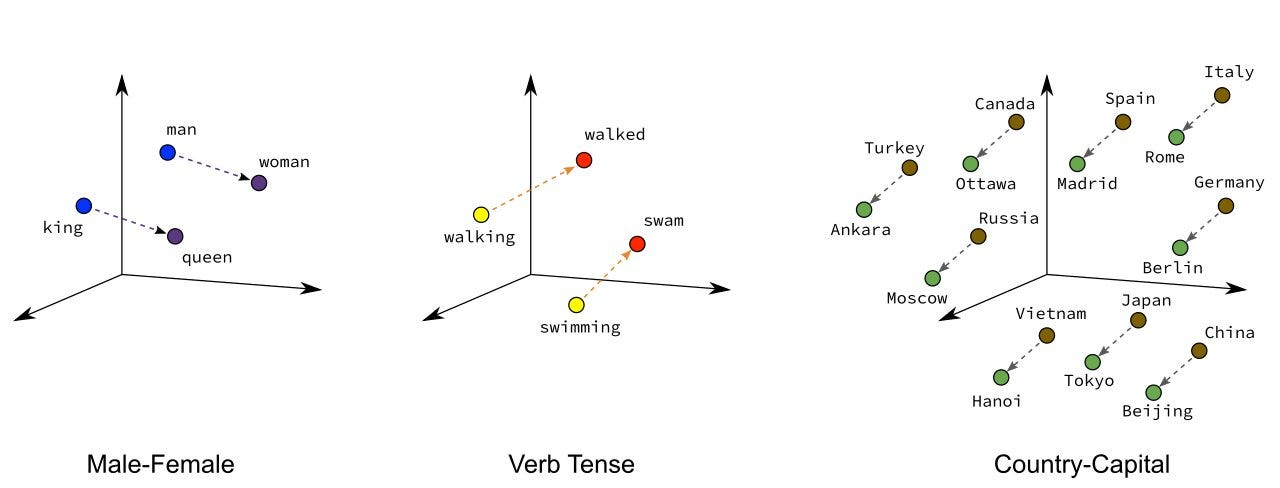
\includegraphics[width=0.8\linewidth]{images/embeddings.jpg}
    \caption{Illustration of potential embeddings, Image from \cite{WordVectors}}
    \label{embeddings}
\end{figure}
Importantly, these embeddings extend beyond representing words in isolation—they evolve through the layers of a transformer to
reflect contextual meaning. For instance, the embedding of “mathematician” could shift to refer specifically to Leibniz, 
depending on the sentence context. While the initial embedding layer does not yet account for surrounding context, it provides 
a foundational semantic representation that is refined throughout the transformer architecture.
(While there are several types of embedding techniques, such as Word2Vec and GloVe, we will not explore them in detail here.)

\subsection{Positional Encoding}
The position of words in a sentence plays a crucial role in understanding their meaning. Early models, such as Recurrent 
Neural Networks (RNNs), inherently capture word order through their sequential processing. However, the Transformer 
architecture does not process tokens sequentially, and therefore lacks an inherent sense of word order. To address this, 
positional encoding is introduced to inject information about the position of each token in the sequence. An effective 
positional encoding scheme should satisfy the following criteria:
\begin{itemize}
    \item \textbf{Unambiguous:} Each position in the sequence should have a unique encoding.
    \item \textbf{Deterministic:} It is beneficial if the encoding follows a predictable mathematical pattern, allowing the 
    model to learn or infer position-based relationships.
    \item \textbf{Distance-aware:} The encoding should enable the model to estimate the relative distance between two 
    positions.
    \item \textbf{Generalizable:} The encoding should allow the model to handle longer sequences than those seen during 
    training. Ideally, values should be bounded to avoid numerical instability.
\end{itemize}
The authors of the \textit{Attention is All You Need} paper \cite{vaswani2023attentionneed} define positional encoding using 
sinusoidal functions as follows:
\begin{gather*}
    f(t)_i = \begin{cases}
        \sin{(\omega_k \cdot t)}, \quad \text{if } i= 2k\\
        \cos{(\omega_k \cdot t)},  \quad \text{if } i= 2k+1
        \end{cases} = \begin{bmatrix}
            \sin{(\omega_{1}\cdot t)} \\
            \cos{(\omega_{1}\cdot t)}\\
            \sin{(\omega_{2}\cdot t)} \\
            \vdots \\
            \sin{(\omega_{d/2}\cdot t)} \\
            \cos{(\omega_{d/2}\cdot t)}\\
         \end{bmatrix}_{d\times 1} \\ 
         \text{with } \omega_k = \frac{1}{10000^{2k/d}}
\end{gather*}
Here, $t$ denotes the position of a token in the sequence (e.g., the 1st, 2nd, or 3rd word), and $d$ is the dimensionality of 
the embedding space. Each dimension of the positional encoding corresponds to a sinusoid with a different frequency.\newline
This encoding is unique as long as the chosen frequencies span a range that exceeds the maximum sequence length $L$ 
(where $t \in \{1, \dots, L\}$). Put simply, at least one dimension must have a sinusoid whose period exceeds $L$, ensuring that 
the function values do not repeat and each position maps to a distinct representation.  Since sine and cosine are 
deterministic functions, the positional encoding is also deterministic. Furthermore, the sinusoidal encoding generalizes well to 
sequences longer than those seen during training, thanks to the periodic nature of sine and cosine functions. Finally, this 
encoding is distance-aware. Because each dimension of the encoding uses a different frequency, the model can infer relative 
positions from the differences between encodings.

\subsubsection{Binary Representation and Positional Encoding}
The intuition behind sinusoidal positional encoding becomes clearer when we consider the binary representation of numbers. At 
first glance, one might wonder how a combination of sine and cosine waves can meaningfully represent position or order. The 
answer lies in how binary counting works.
\begin{figure}[H]
    \centering
    \begin{minipage}[t]{0.25\textwidth}
     \vspace{2cm}
        \centering
        \begin{tabular}{c|c}
        \textbf{0:} 0000 & \textbf{8:} 1000 \\
        \textbf{1:} 0001 & \textbf{9:} 1001 \\
        \textbf{2:} 0010 & \textbf{10:} 1010 \\
        \textbf{3:} 0011 & \textbf{11:} 1011 \\
        \textbf{4:} 0100 & \textbf{12:} 1100 \\
        \textbf{5:} 0101 & \textbf{13:} 1101 \\
        \textbf{6:} 0110 & \textbf{14:} 1110 \\
        \textbf{7:} 0111 & \textbf{15:} 1111 \\
        \end{tabular}
    \end{minipage}%
    \hfill
    \begin{minipage}[t]{0.75\textwidth}
     \vspace{0pt}
        \centering
        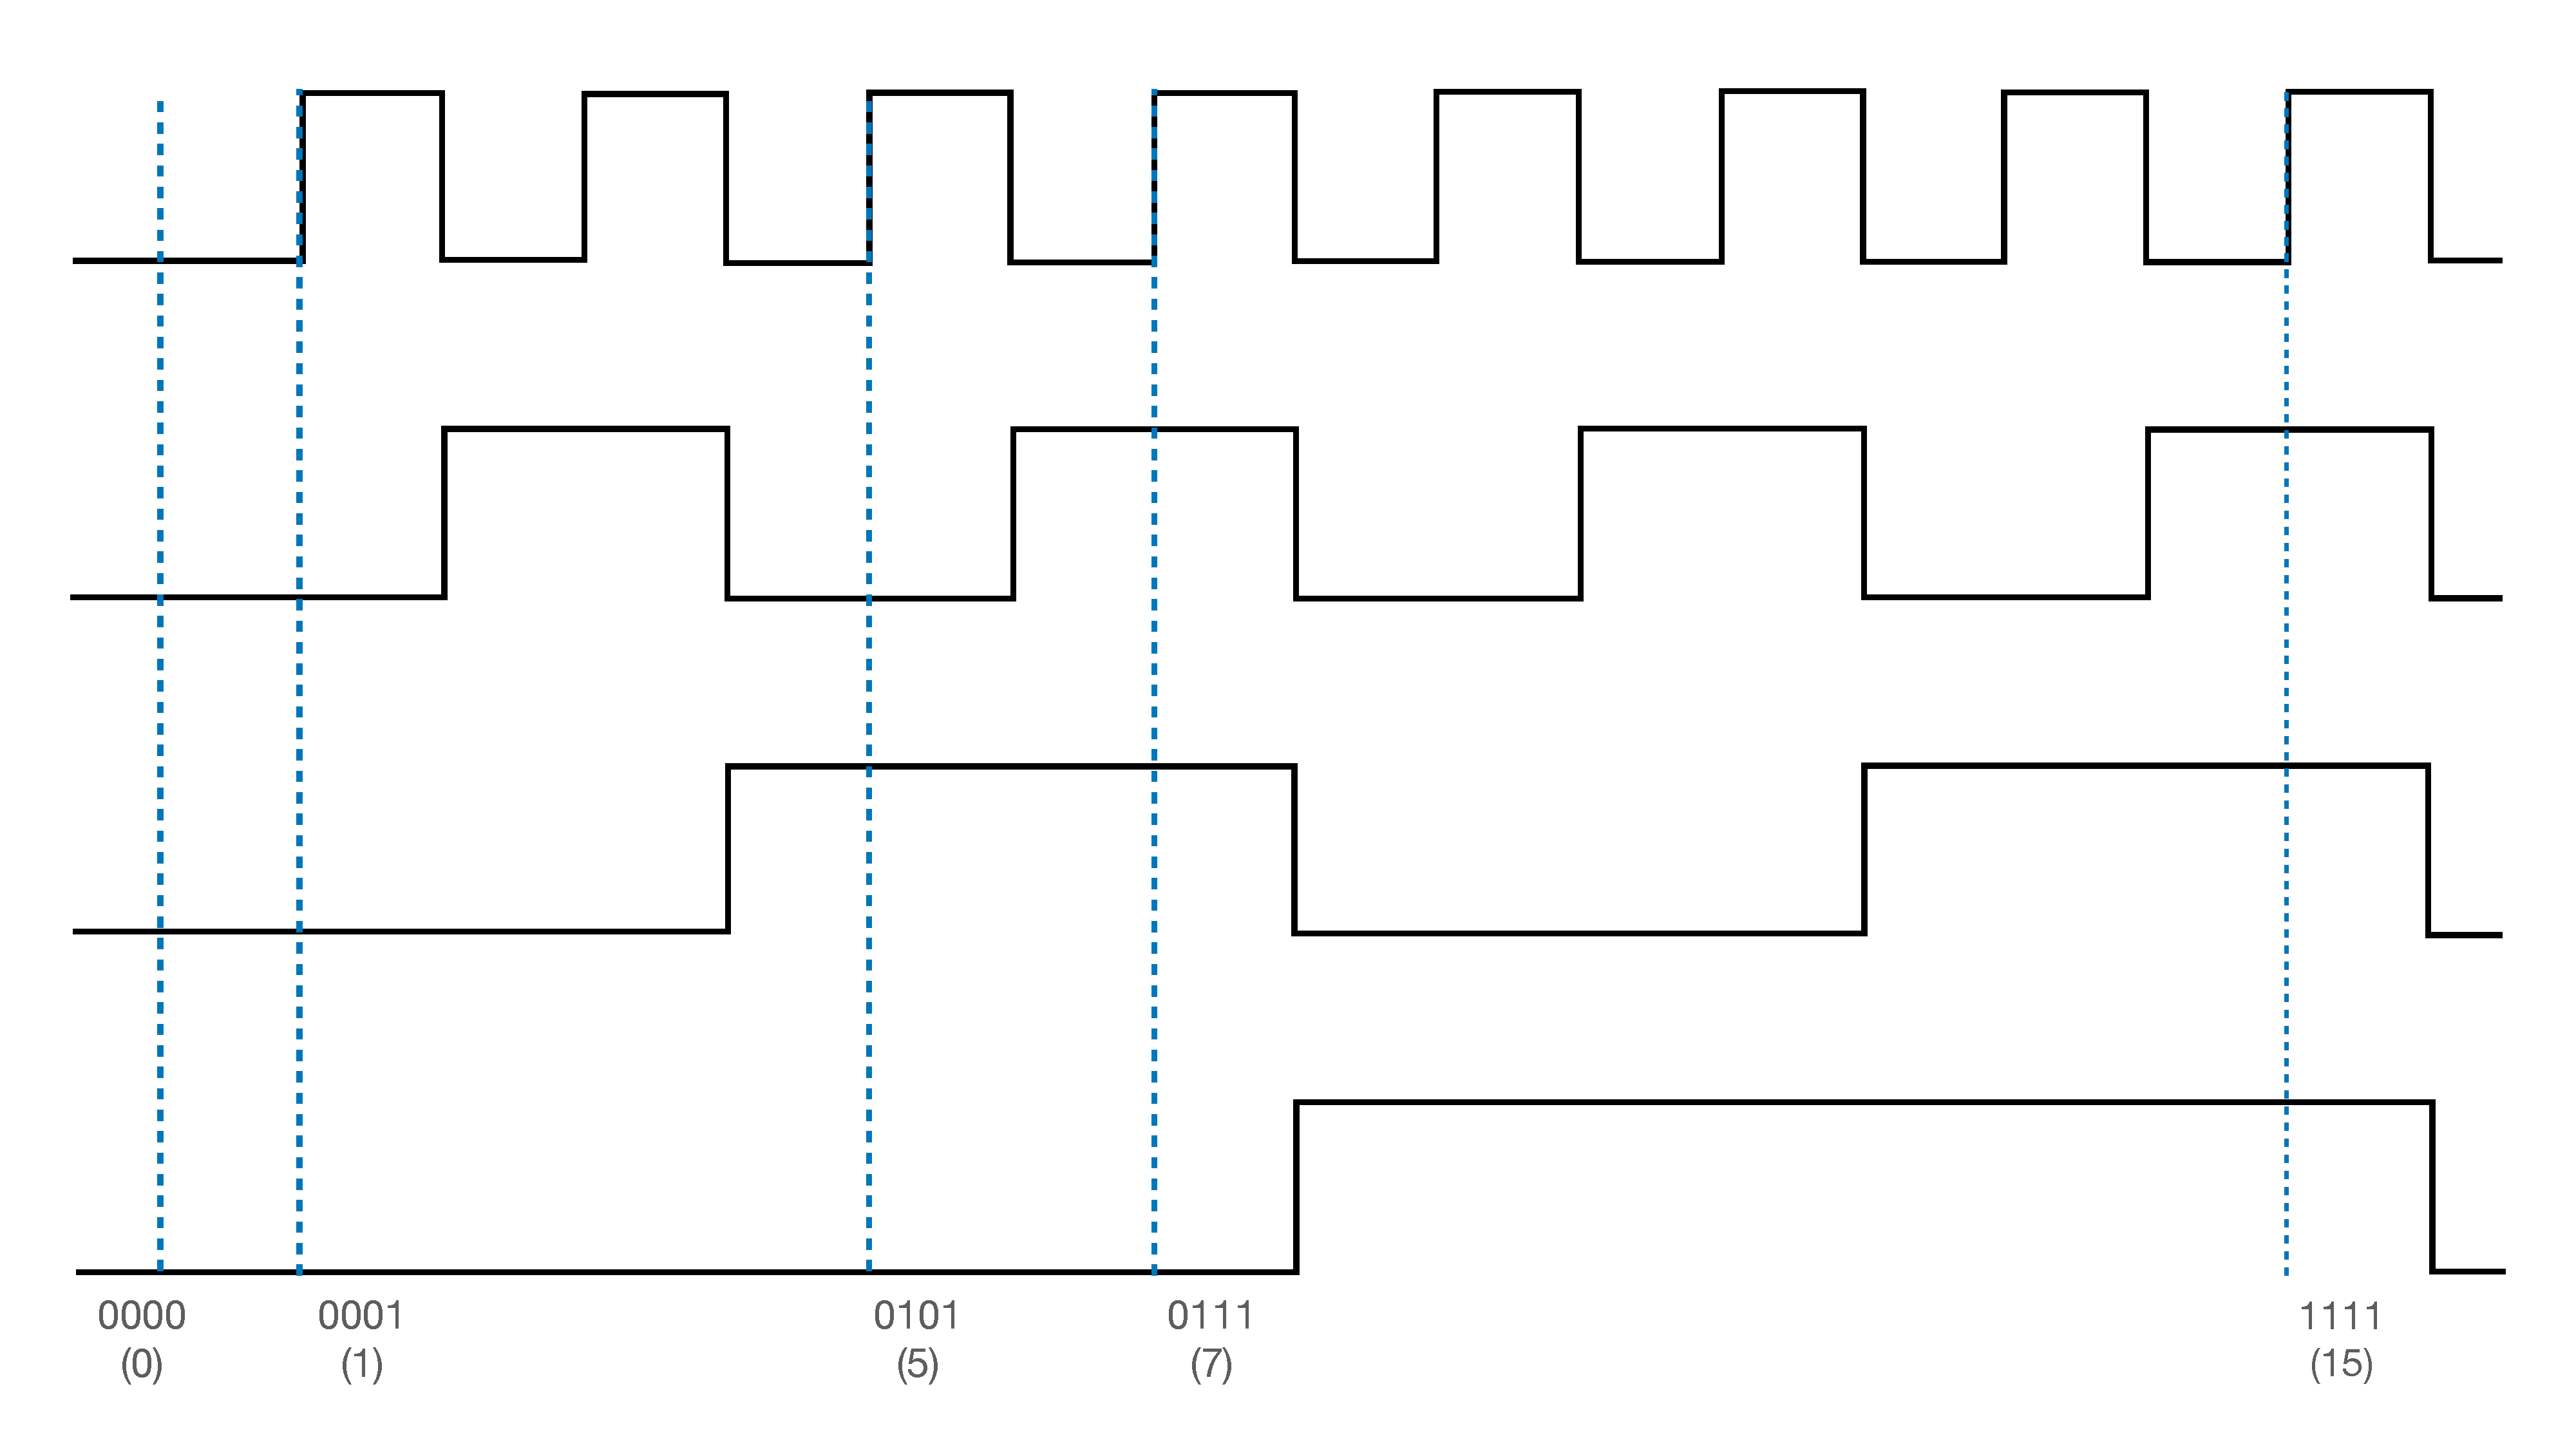
\includegraphics[width=\linewidth]{images/4_bit_counter.pdf}
        %\caption{4-bit binary counter waveform visualization.}
        \label{fig:4bit-counter}
    \end{minipage}
    \caption{Illustration of the 4-bit binary number system. On the left is the binary representation in tabular form, and on 
    the right is a visualization using periodic step functions (square waves).}
\end{figure}
\vspace{-0.3cm}
So, we can use periodic wave functions (one for each dimension) to encode numbers. This idea closely resembles the sine and 
cosine functions used in positional encoding. Using discrete binary values directly would be inefficient in the continuous 
space of neural networks. Instead, we use their smooth, differentiable counterparts: sinusoidal functions. These functions act 
as continuous analogues of alternating bits. By varying their frequencies we mimic the behaviour of binary bits flipping at 
different rates. This allows the model to infer both absolute position and relative distance, all within a compact and expressive 
representation.
\begin{figure}[H]
\hspace{1.5cm}
    %\centering
    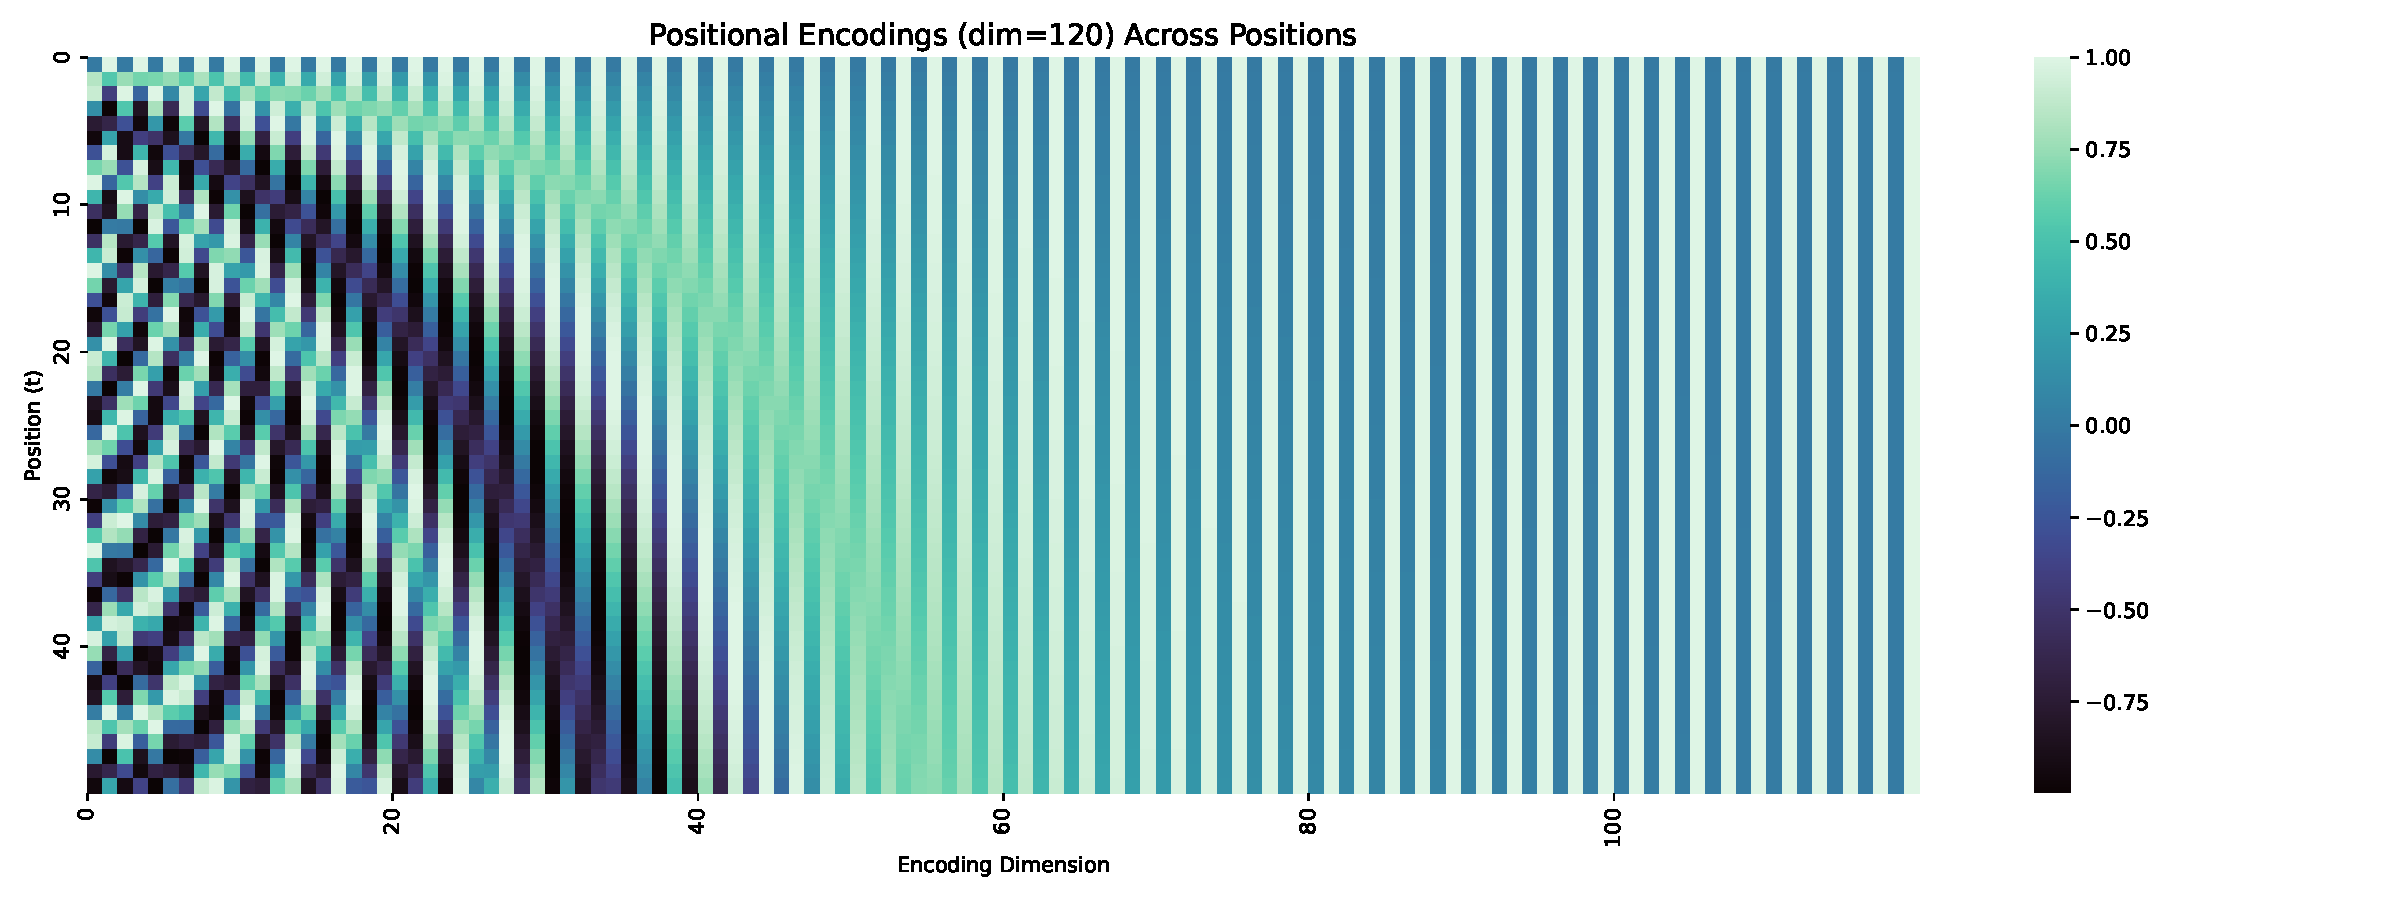
\includegraphics[width=0.92\linewidth]{images/pos_enc_visual.pdf}
   \caption{Visualization of positional encodings for positions 0 to 49 with an encoding dimension of 120. Each row represents 
   the positional encoding for one position, and each column corresponds to a specific dimension with its associated value.}
    \label{fig:pos_enc_vis}
\end{figure}
\subsection{Attention Mechanism}
In a transformer model, the key objective is for embeddings (vectors) to not only represent individual words 
but also capture context, allowing for a more nuanced understanding of language. This is achieved through 
the self-attention mechanism. To understand this, let's first break down a simple example and build on it.
Let's consider a sentence like ''Kings made laws to keep power over the small towns`` and focus on how the 
attention mechanism works. Each word is initially represented as an embedding vector $\vec{E}_i$.

\subsubsection{Query, Key, and Value Vectors}
From each embedding $\vec{E}_i$, three vectors are computed using learned weight matrices: 
\begin{itemize} 
\item $\vec{Q}_i = W_Q \vec{E}_i$ (Query) 
\item $\vec{K}_i = W_K \vec{E}_i$ (Key) 
\item $\vec{V}_i = W_V \vec{E}_i$ (Value) 
\end{itemize}
These vectors will determine how a token attends to others in the sequence.

\subsubsection{Attention Scores}
The next step is to measure the relevance of the different tokens in relation to each other. This is done by 
computing the dot product between the query vector of one word and the key vectors of all other words. The 
dot product gives a measure of similarity: high positive value indicates that the two words are more relevant to 
each other in the context (vectors pointing in nearly the same direction) while negative values indicate that the words
are not so relevant to each other (vectors nearly pointing in opposite directions).

\subsubsection{Softmax}
After computing the dot product, we apply a softmax operation to the values. This converts the raw scores 
into probabilities, allowing the model to focus more on the most relevant words and ignore less relevant 
ones.\newline
Additionally, in some settings (e.g., in reinforcement learning), we may mask certain values in the 
attention matrix, ensuring that later words do not influence earlier ones. This is done by setting specific
values to negative infinity before applying softmax, which effectively eliminates their contribution.

\subsubsection{Updating the Embedding}
Now that we know which words are important for each other, the next step is to update the embeddings. The 
update is based on the value matrix, which is another learned weight matrix. The value matrix is multiplied 
by each word’s embedding, and the resulting vectors are summed to produce the final output.\newline
The value matrix answers the question: If this word is relevant to adjusting the meaning of another word, what specific adjustments should be made? This results in a new set of embeddings that reflect the context. The whole attention procedure 
can be described via the function $$\text{Attention}(Q,K,V) = \text{softmax}\left(\frac{QK^T}{\sqrt{d_k}}\right)V$$
To understand why the attention scores are scaled by $\sqrt{d_k}$, consider the dot product between a 
query vector $\vec{q}_i$ and a key vector $\vec{k}_j$:
$$\sigma_{ij} = \vec{q}_i \cdot \vec{k}_j = \sum_{n=1}^{d_k} q_{in} k_{jn}$$
If we assume that the components of $\vec{q}_i$ and $\vec{k}_j$ are independent, have zero mean, and unit variance (we can 
make the assumption due to the use of LayerNorm), then each term in the sum $q_{in} k_{jn}$ will have mean zero and variance 
1. Therefore, the variance of the sum (i.e., the dot product) becomes:
$$\text{Var}(\sigma_{ij}) = \sum_{n=1}^{d_k} \text{Var}(q_{in} k_{jn}) = d_k \longrightarrow 
\text{std}(\alpha_{ij}) = \sqrt{d_k}$$
This means the standard deviation of the attention score grows with the square root of the key dimension. The normalization 
ensures that the variance of the attention scores remains approximately constant, regardless of dimensionality, leading to 
more stable gradients and more effective learning.
\begin{figure}[H]
  \centering
  \begin{minipage}[b]{0.45\linewidth}
    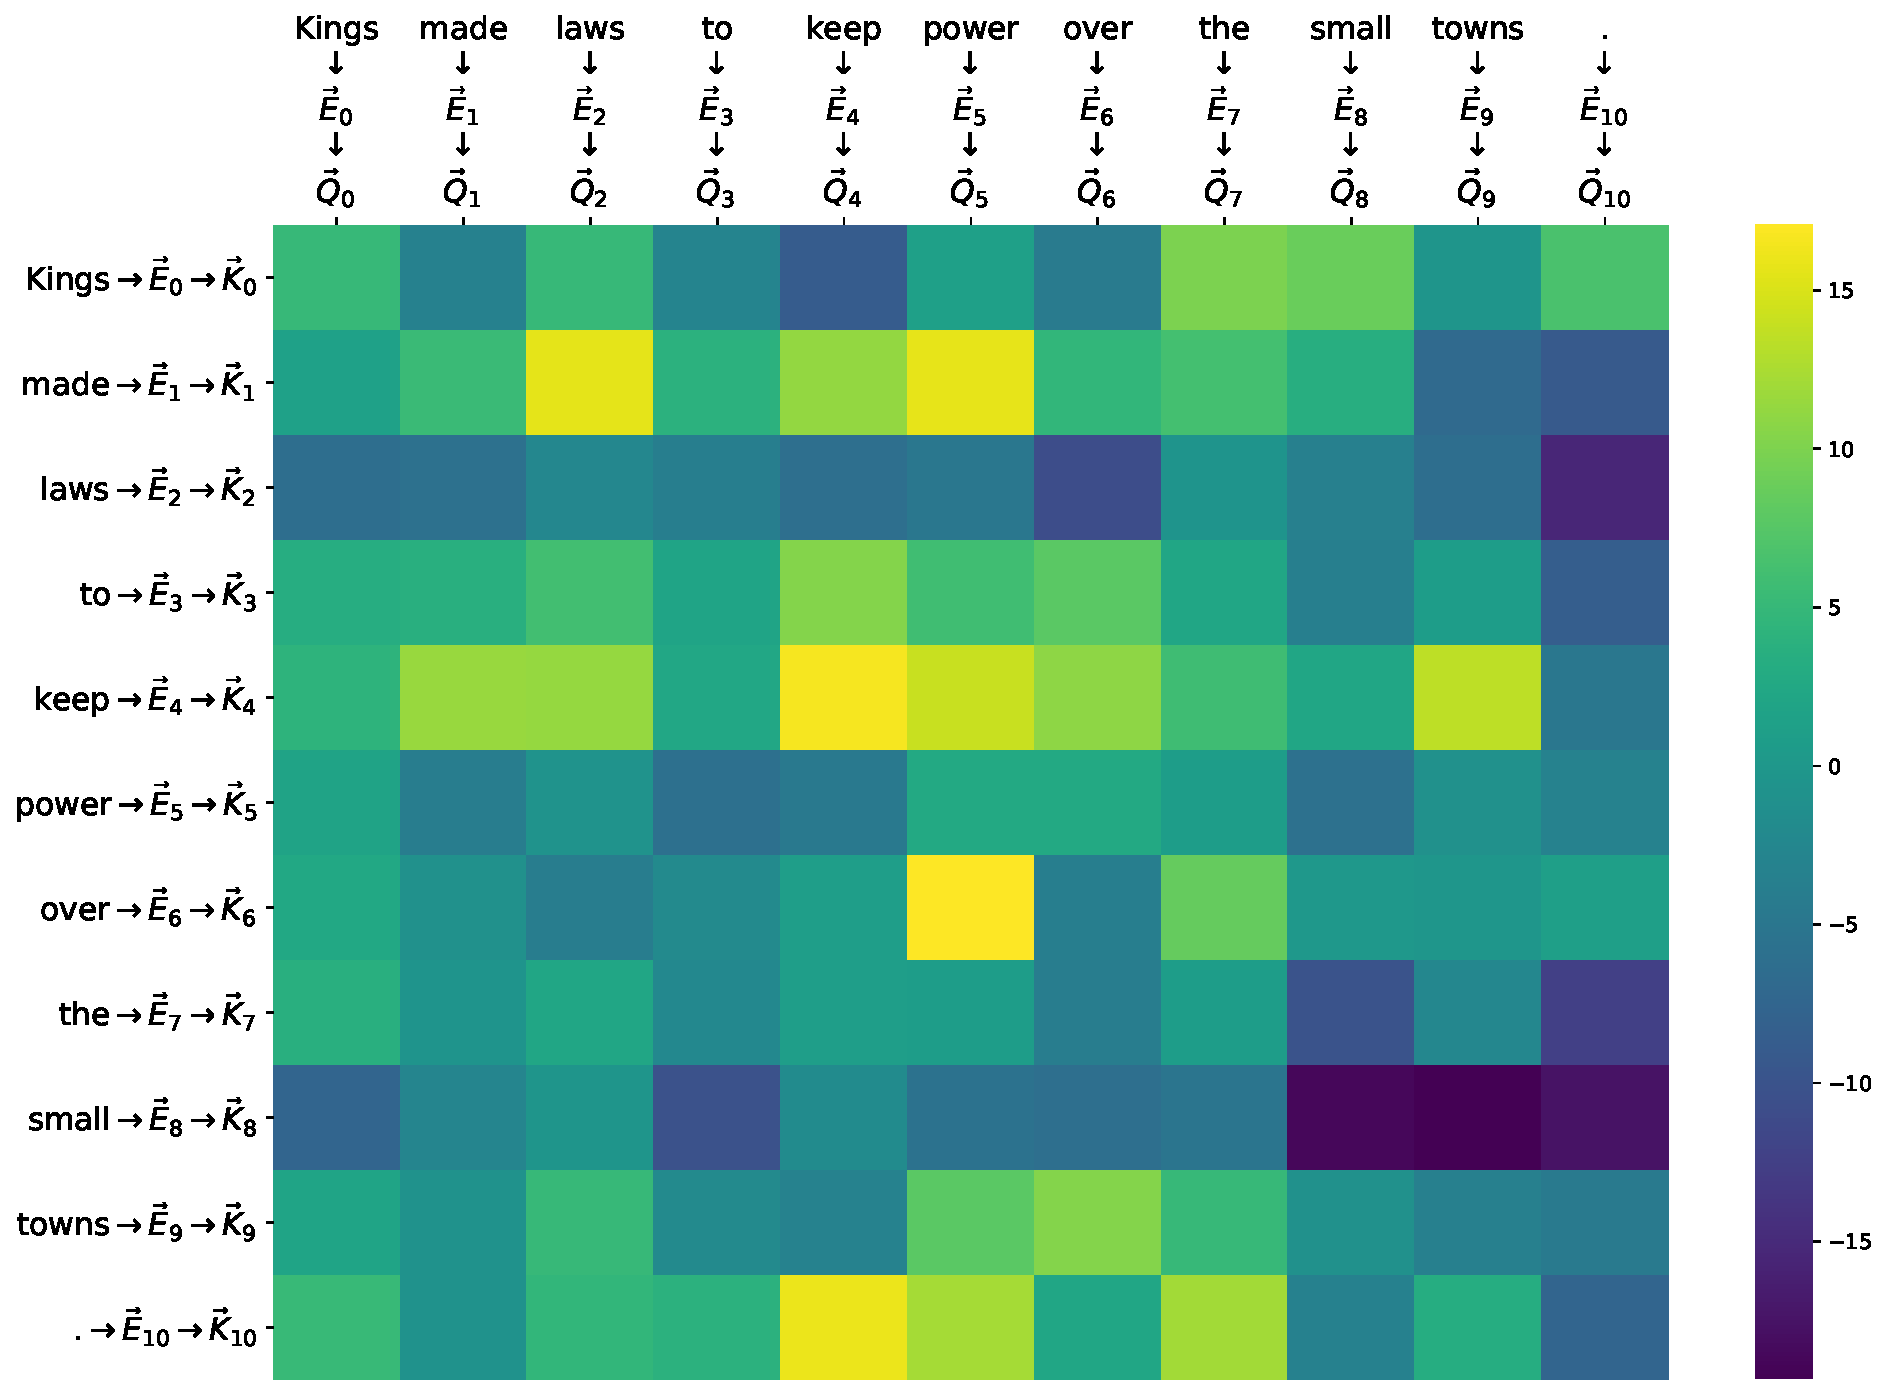
\includegraphics[width=\linewidth]{images/normal_attn.pdf}
  \end{minipage}
  \hfill
  \begin{minipage}[b]{0.45\linewidth}
    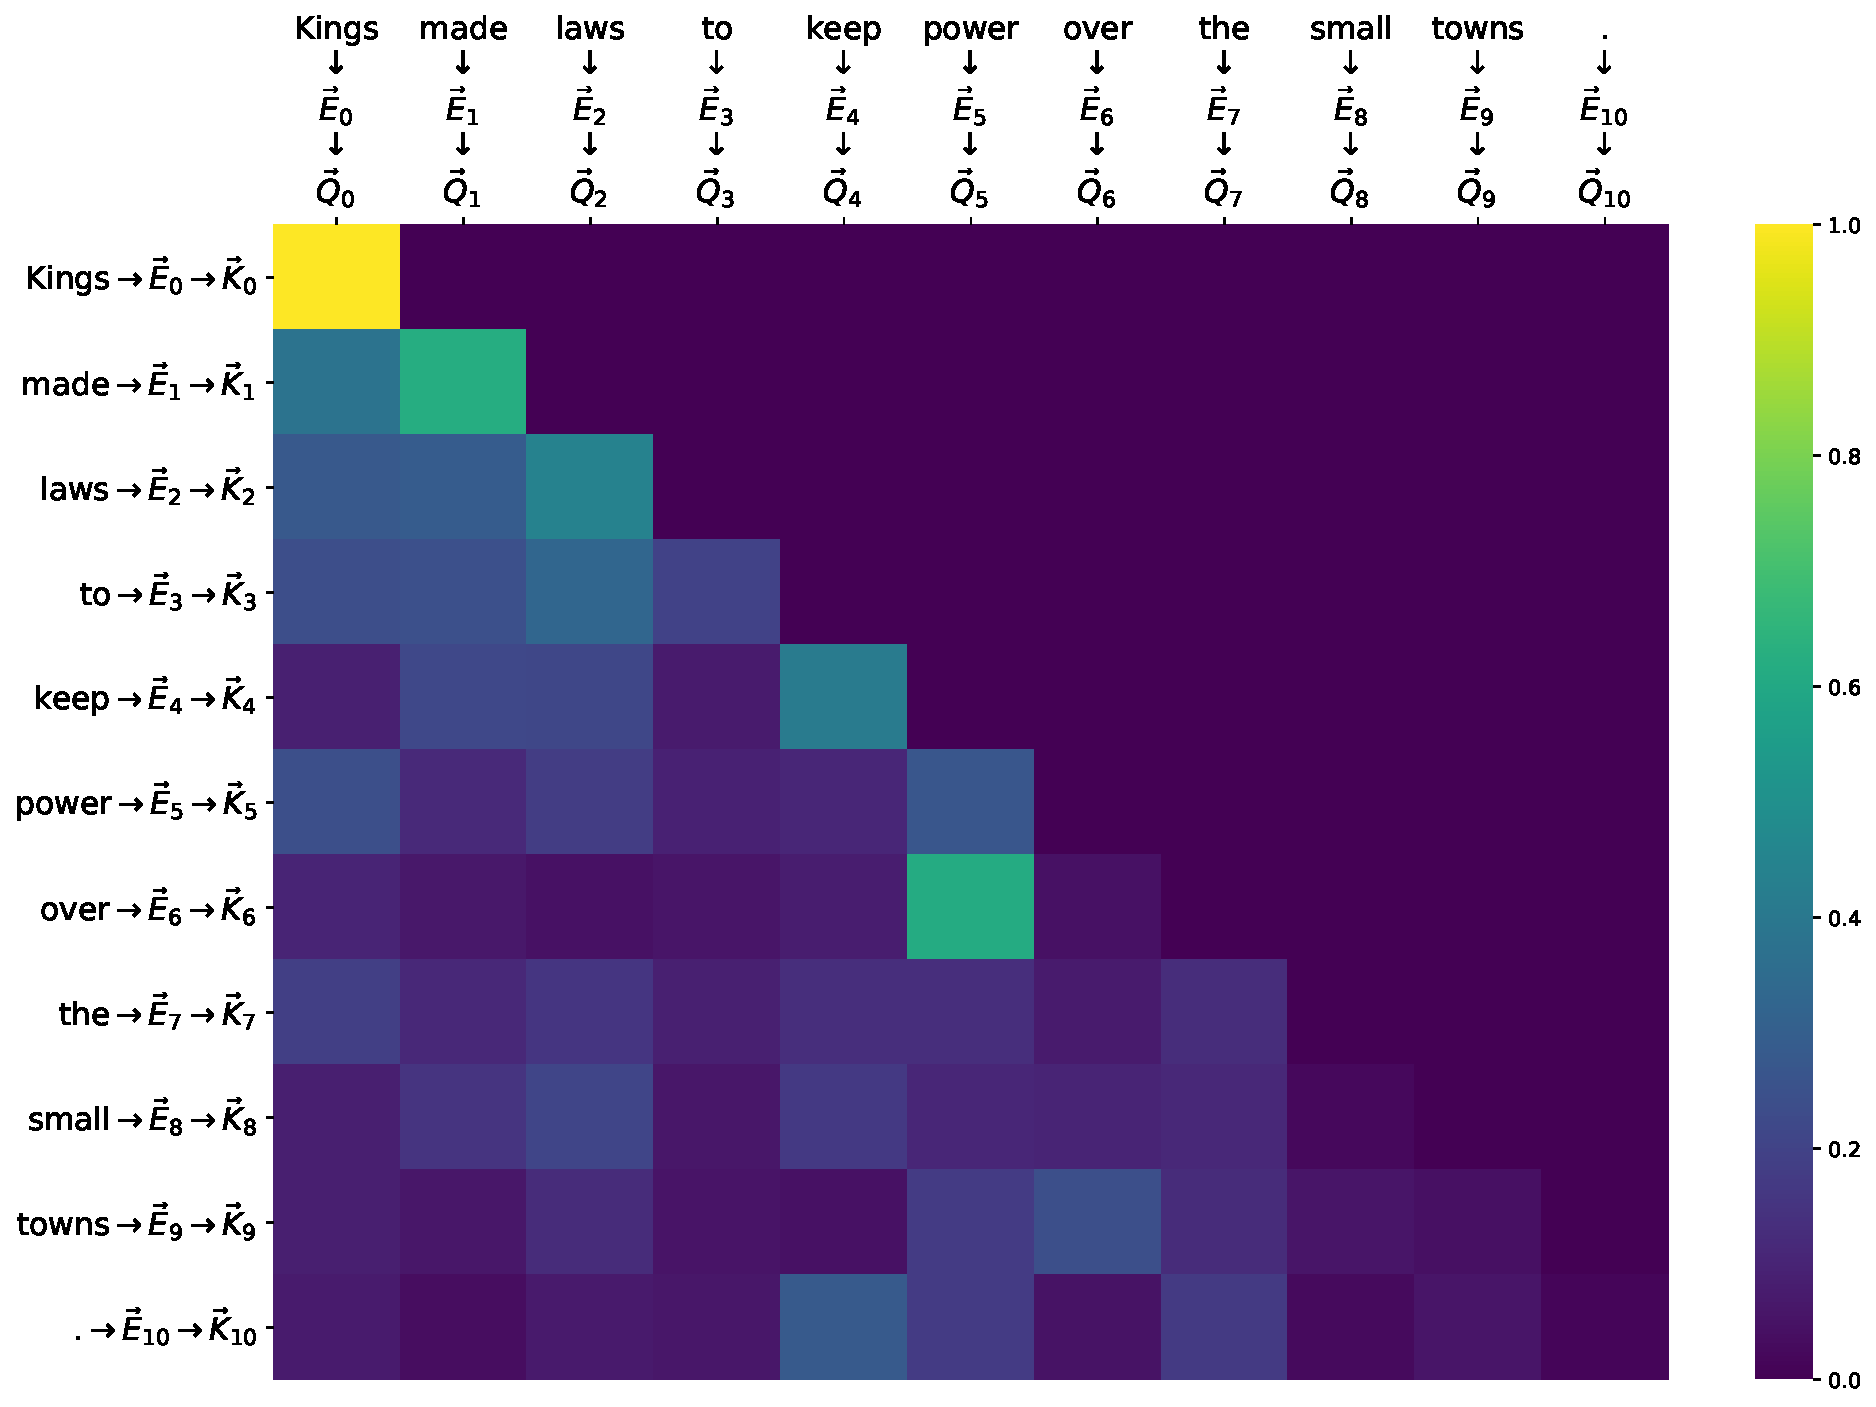
\includegraphics[width=\linewidth]{images/mod_attn.pdf}
  \end{minipage}
\caption{Illustration of the attention patterns from the first attention head in the first layer of GPT-2, for the input text: 
\textit{''Kings made laws to keep power over the small towns.``} The left plot shows the raw attention scores ($QK^T$), while 
the right plot displays the masked and scaled attention weights after applying the softmax function, i.e., 
$\text{softmax}\left(\frac{QK^T}{\sqrt{d_k}}\right)$.}
\end{figure}

\subsubsection{Multi-Head Attention}
The process described above outlines a single ''head`` of attention, where each word attends to other words 
based on their relevance. However, in practice, we use multi-head attention, which runs multiple attention 
mechanisms in parallel, each with its own learned query, key, and value matrices.\newline
The benefit of multi-head attention is that it allows the model to focus on different aspects of the input 
simultaneously. For instance, one head might focus on syntactic relationships, while another might focus on 
semantic meanings, and yet another could capture long-range dependencies. This parallel processing allows 
the transformer to learn richer, more nuanced representations.\newline
To make this process more efficient, each attention head typically uses smaller key, value, and query 
matrices. After the attention 
outputs are computed using these smaller matrices, the results from all heads are concatenated and passed 
through a linear layer to combine them. The formula for a Multi-Head attention block with $k$ heads is given by 
$$\text{MultiHead}(Q,K,V)=\text{Concat}[\text{head}_1,\dots,\text{head}_k]W_O$$
where $W_O$ is the learnable output projection matrix of dimension $(k\cdot d_h) \times d_\text{model}$
with $d_h$ being the dimensionality of the value vectors (the same as the dimensionality of each head's output) and
$d_\text{model}$  the final desired output dimensionality of the multi-head attention (usually equal to the 
model's embedding size).
\begin{figure}[H]
    \centering
    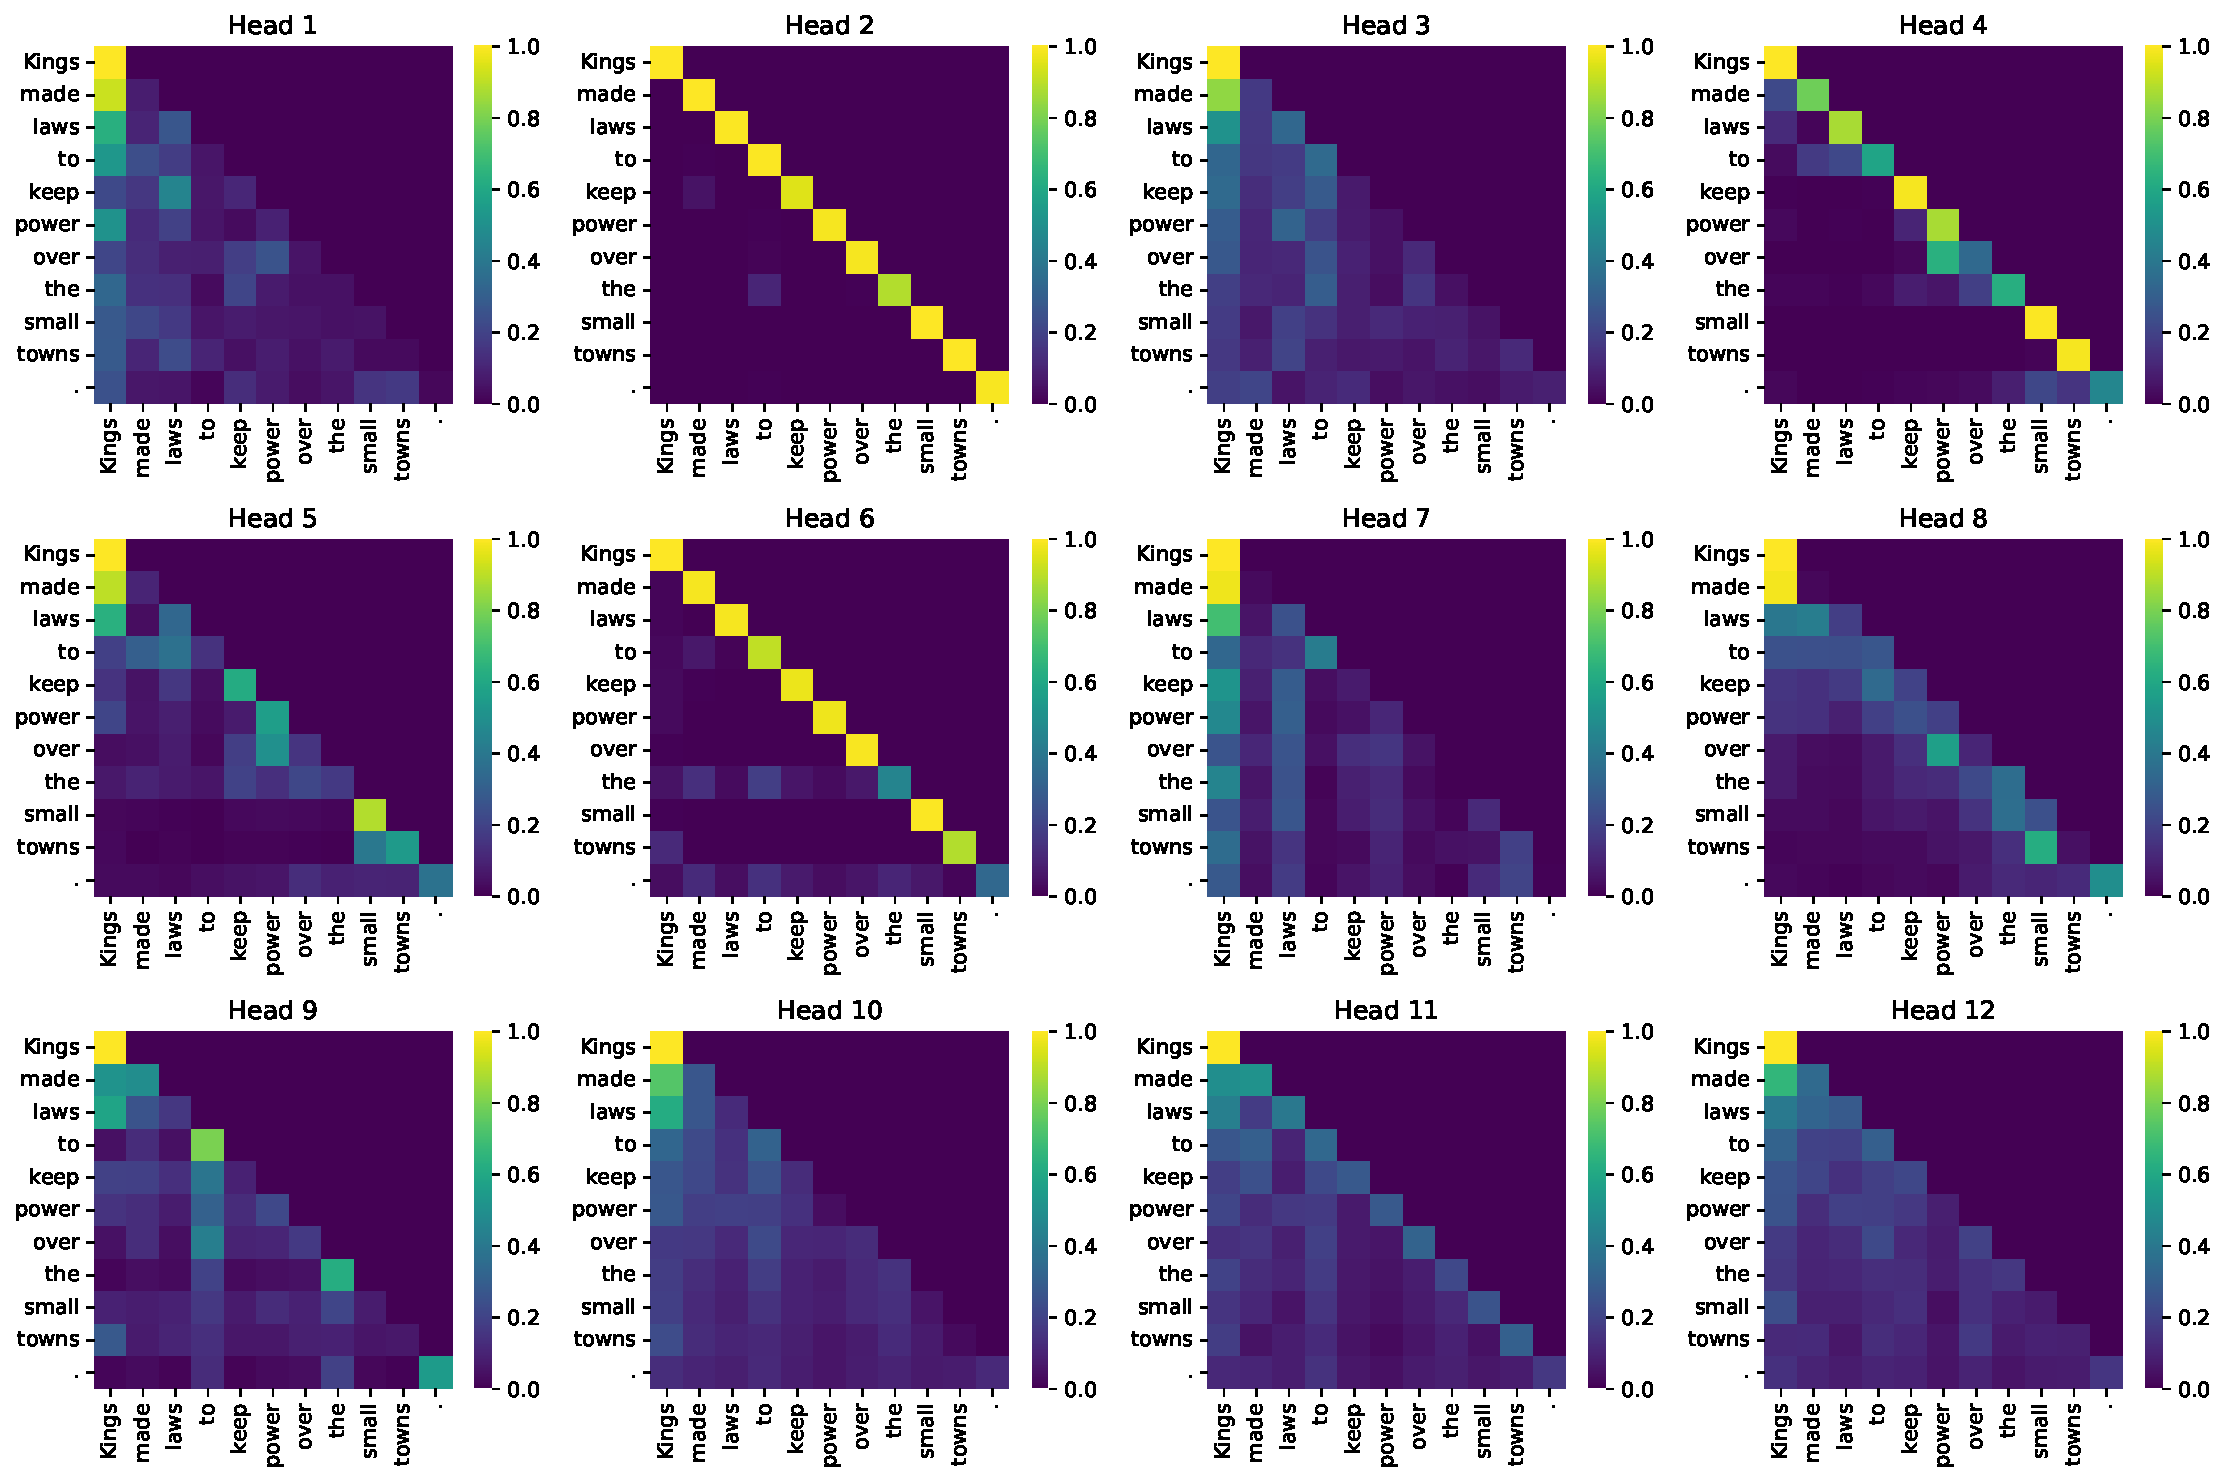
\includegraphics[width=0.8\linewidth]{images/multi_head_attn.pdf}
  \caption{Illustration of the attention patterns from all heads in the first layer of GPT-2 for the sentence: \textit{"Kings 
  made laws to keep power over the small towns."}}
\end{figure}

\subsection{Feedforward Neural Network and Add \& Norm}
The Feedforward Neural Network (FNN) in Transformers is a simple multi-layer perceptron (MLP) composed of fully connected 
layers with ReLU activations.\newline
The "Add" operation refers to residual (skip) connections, which are critical for stabilizing deep networks. Without them, 
models can suffer from vanishing or exploding gradients, making training inefficient or unstable. Residual connections allow 
gradients to flow more directly through the network and help mitigate the degradation problem, where adding more layers leads 
to worse performance. \newline 
Normalization further stabilizes training by ensuring that inputs to each layer are centered and appropriately scaled. While 
Batch Normalization (BN) normalizes across the batch dimension, it is less suitable for Transformer architectures, which often 
work with variable-length sequences and small batch sizes. Instead, Transformers use Layer Normalization (LN), which 
normalizes across feature dimensions for each individual sequence. This approach is more robust in the context of sequence modeling.

\subsection{Modifications to the Vanilla Transformer}
While the original transformer architecture has demonstrated strong performance across a range of tasks, it also faces certain 
limitations particularly when modeling long sequences. In this section, we examine follow-up work that addresses these issues.


\subsubsection{Transformer-XL}
Transformers are capable of learning long-term dependencies, but they are limited by a 
fixed-length context when applied to language modelling tasks. Transformer-XL 
\cite{dai2019transformerxlattentivelanguagemodels} proposes an 
architecture that extends this capability by enabling the learning of dependencies beyond 
a fixed length, without disrupting temporal coherence. This is achieved by incorporating a 
memory mechanism into the transformer model.\newline
The approach begins by splitting the input into segments, denoted as $X_i$. If we were to 
process these segments using a standard transformer model, there would be no attention 
between them, as illustrated in Figure \ref{fig:vanilla}.\newline 
To overcome this, Transformer-XL concatenates the hidden states from the previous segment with the current input at every 
transformer layer. These past states are treated as fixed memory i.e. gradients are not propagated through 
them allowing efficient reuse without increasing memory cost during backpropagation. This approach is illustrated in 
Figure \ref{fig:xl}.
\begin{figure*}[!h]
	\begin{subfigure}[b]{0.292\linewidth}
		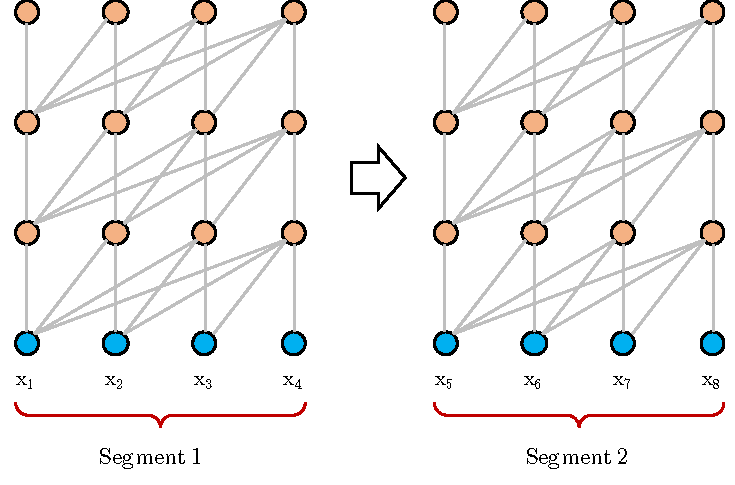
\includegraphics[width=\textwidth]{images/vanilla-train.pdf}
		\caption{\small Train phase.}
		\label{fig:vanilla-train}
	\end{subfigure}
	\rulesep
	\begin{subfigure}[b]{0.69\linewidth}
		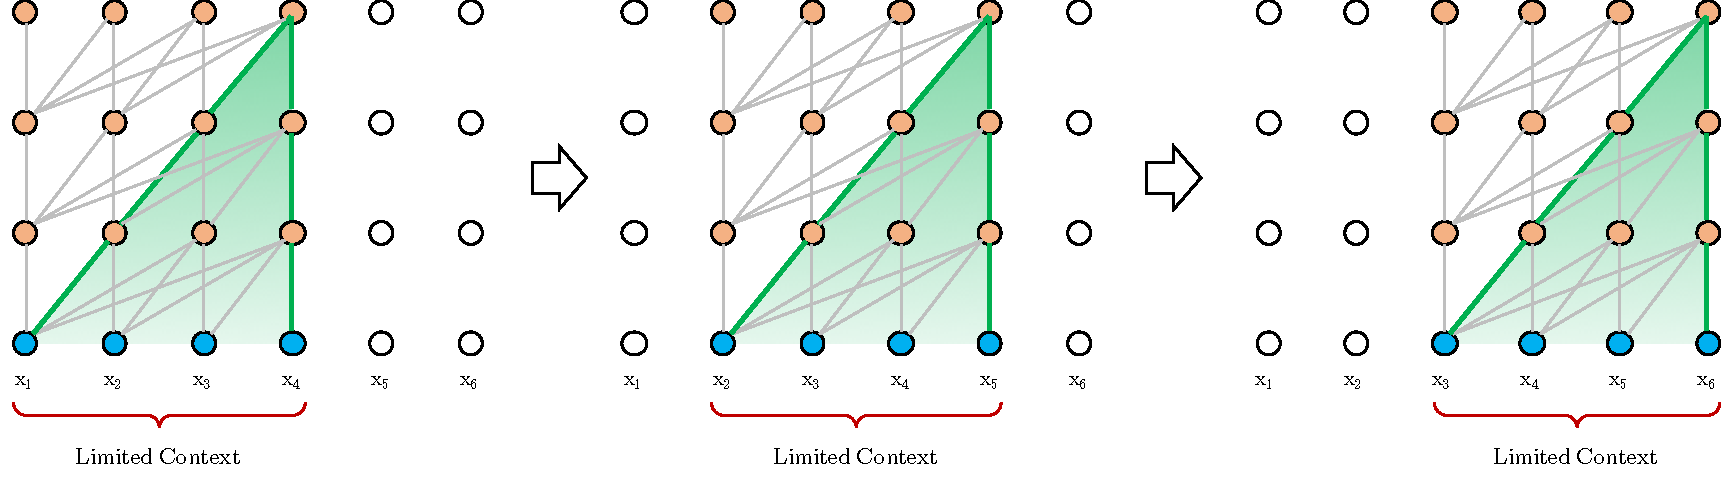
\includegraphics[width=\textwidth]{images/vanilla-eval.pdf}
		\caption{\small Evaluation phase.}
		\label{fig:vanilla-eval}
	\end{subfigure}
	\caption{\small Illustration of the vanilla transformer model with a segment length 4. \cite{dai2019transformerxlattentivelanguagemodels}}
	\label{fig:vanilla}
\end{figure*}

\begin{figure*}[!h]
	\begin{subfigure}[b]{0.62\linewidth}
		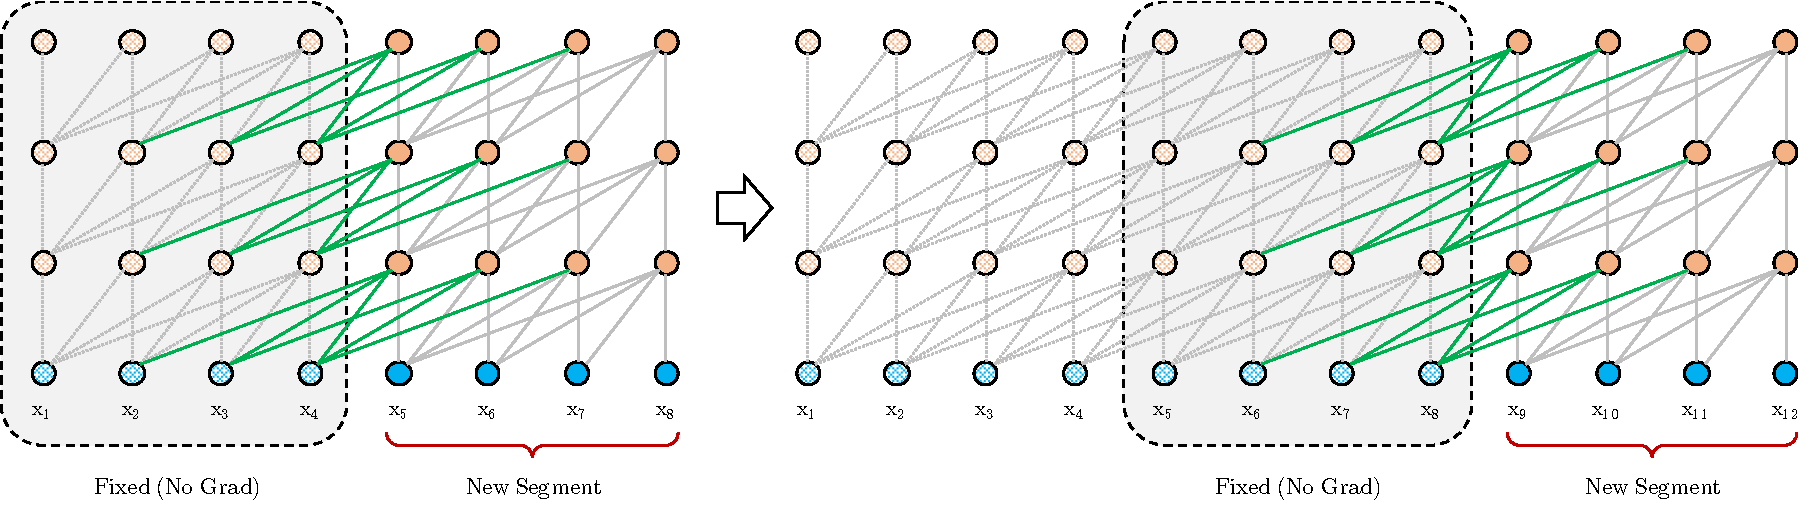
\includegraphics[width=\textwidth]{images/xl-train.pdf}
		\caption{\small Training phase.}
		\label{fig:xl-train}
	\end{subfigure}
	\rulesep
	\begin{subfigure}[b]{0.35\linewidth}
		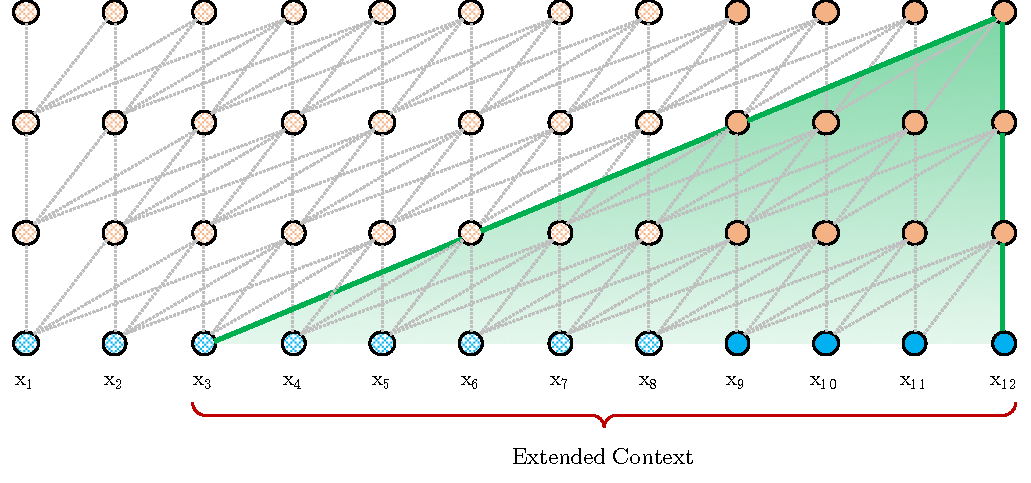
\includegraphics[width=\textwidth]{images/xl-eval.pdf}
		\caption{\small Evaluation phase.}
		\label{fig:xl-eval}
	\end{subfigure}
	\caption{\small Illustration of the Transformer-XL model with a segment length 4. \cite{dai2019transformerxlattentivelanguagemodels}}
	\label{fig:xl}
\end{figure*}
However, this modification introduces a new challenge: absolute positional encodings used in vanilla transformers cannot 
correctly handle segment-level continuity. For example, tokens $X_1^1$ (from one segment) and $X_1^2$ (from the next) would 
receive identical positional encodings, despite being temporally distinct. This breaks the sequence order and confuses the 
model.\newline
To solve this, Transformer-XL replaces absolute positional encodings with relative positional encodings. This allows the model 
to compute attention based on the relative distance between tokens, preserving the temporal relationships across segments. For
implementation details, refer to Section 3.3 in the original paper \cite{dai2019transformerxlattentivelanguagemodels}.

\subsubsection{Stabilizing Transformers for Reinforcement Learning}
Despite their success in NLP and vision, vanilla transformers and their memory-augmented variants 
like Transformer-XL initially performed poorly in reinforcement learning (RL) settings. For instance, 
\cite{mishra2018simpleneuralattentivemetalearner} found that standard transformers failed on even basic 
bandit problems and tabular Markov Decision Processes (MDPs), suggesting that transformers may not be 
well-suited for RL without further adaptation.\newline 
To address this, \cite{parisotto2019stabilizingtransformersreinforcementlearning} proposed modifications that significantly 
improve transformer stability and performance in RL. Their work builds on Transformer-XL and introduces two key changes.

\paragraph{1. TrXL-I: Input-Normalized Transformer-XL} The first modification is reordering the application of layer 
normalization. Instead of applying it before and after each submodule (as in the original transformer), it is applied only to 
the inputs. This reordering creates an identity map from the input of the transformer at the first layer to the output at the 
last layer, unlike the canonical transformer, which applies multiple layer normalization operations that non-linearly 
transform the state encoding.\newline
TrXL-I shows a significant improvement in stability and performance over TrXL. One 
hypothesis for this improvement is that, with the initialization of submodules producing 
values near zero, the state encoding is passed untransformed to the policy and value 
heads. This allows the agent to learn a Markovian policies first e.g. 
$\pi(a | s_1, ..., s_n) \approx \pi(a | s_n)$ before gradually incorporating longer-term memory, 
which aligns with how agents typically learn: basic behaviors precede memory-dependent 
strategies.\cite{parisotto2019stabilizingtransformersreinforcementlearning}

\paragraph{2. GTrXL: Gated Transformer-XL} To further stabilize learning, the authors replace standard residual connections 
with gated residual layers, inspired by gating mechanisms in LSTMs. This results in the Gated Transformer-XL (GTrXL) 
architecture. Gating enables dynamic control over how much information is retained or suppressed at each layer, improving both 
optimization and generalization.\newline 
For a detailed explanation of how the gating block is defined, refer to the original paper 
\cite{parisotto2019stabilizingtransformersreinforcementlearning}. The authors explore various gating functions—similar to 
A helpful supplementary resource on gating mechanisms in neural networks can be found 
\href{https://medium.com/autonomous-agents/a-math-deep-dive-on-gating-in-neural-architectures-b49775810dde}{see})

\begin{figure}[H]
    \centering
    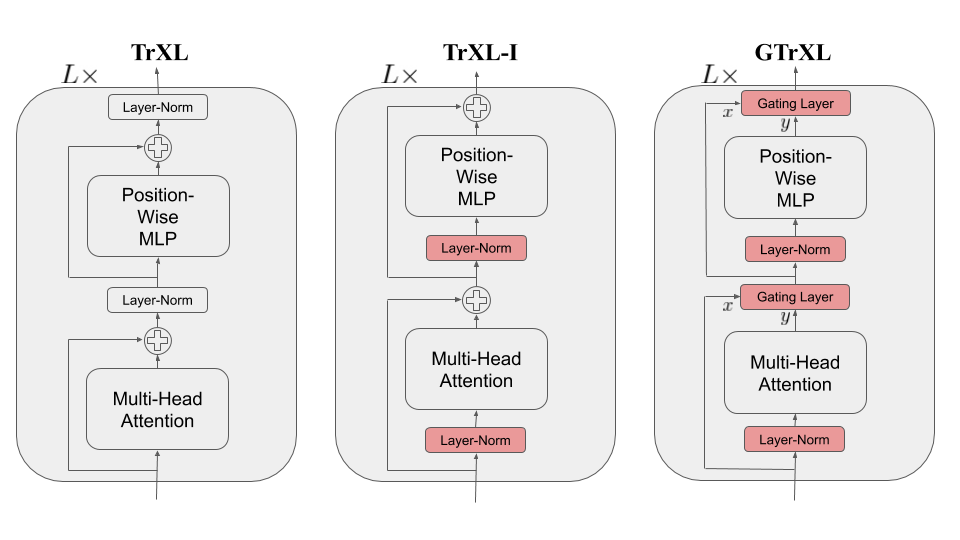
\includegraphics[width=0.7\linewidth]{images/gtrxl.png}
    \caption{Visualisation of the modified Transformer-XL block from \cite{parisotto2019stabilizingtransformersreinforcementlearning}}
    \label{fig:gtrxl}
\end{figure}

\subsection{Transformers in RL}
While this section does not cover all transformer-based approaches in reinforcement learning, several notable works are worth 
highlighting for further reading. Decision Transformer \cite{chen2021decisiontransformerreinforcementlearning} introduced a novel 
framing of reinforcement learning as a sequence modeling problem, treating trajectories as input-output sequences. More recently, 
PoliFormer \cite{poliformer2024} demonstrated that scaling on-policy RL with transformer architectures can produce highly capable 
agents, particularly in navigation tasks.

\subsection{Pros and Cons of Transformers in RL}
Transformer-based models in RL offer several advantages. They are well-suited for evaluating memory and credit assignment 
capabilities, and they tend to perform strongly on tasks that require long-term memory. However, they do not inherently improve 
long-term credit assignment and often suffer from poor sample efficiency. Additionally, many existing RL benchmarks that aim to 
test memory or credit assignment often conflate the two or rely on tasks with predominantly short-term dependencies, limiting the 
insights that can be drawn about transformers' strengths in truly long-horizon settings.

\subsection{Resources}
There are several excellent resources for learning about transformers. A particularly insightful video series is the Neural 
Networks series by 3Blue1Brown, which includes a well-explained introduction to transformers \cite{3ble1brownNN}. Another highly 
recommended resource is Lilian Weng’s blog post, Attention? Attention! \cite{weng2018attention}, which provides a clear and 
intuitive breakdown of the underlying mechanisms.


%\begin{table}[H]
%\begin{tabularx}{\linewidth}{>{\parskip1ex}X@{\kern4\tabcolsep}>{\parskip1ex}X}
%\toprule
%\hfil\bfseries Transformer
%&
%\hfil\bfseries RNN
%\\\cmidrule(r{3\tabcolsep}){1-1}\cmidrule(l{-\tabcolsep}){2-2}

%% PROS, separated by empty line or \par
%Transformers, using self-attention, process all tokens simultaneously, speeding up training and inference. \par
%Transformers' self-attention allows tokens to attend to each other directly, efficiently capturing long-range dependencies. %\par

%&
%
%% CONS, separated by empty line or \par
%RNNs process data sequentially, limiting parallelization and slowing training. \par
%RNNs struggle with long sequences due to vanishing gradients. \par

%\\\bottomrule
%\end{tabularx}
%\end{table}


\section{Generative Models}
Generative models aim to learn the underlying probability distribution of data, enabling them to generate 
new samples that closely resemble those in the training set. Unlike discriminative models, which focus on 
modeling the conditional probability $p(y|x)$ to find decision boundaries between classes,  generative models
learn the joint distribution $p(x,y)$, typically by modeling $p(x|y)$  along with the class prior $p(y)$.
Additionally, once trained, generative models can be employed for classification tasks using Bayes' theorem:
$$p(y|x) = \frac{p(x|y)p(y)}{p(x)} = \frac{p(x|y)p(y)}{\sum_{y}p(x|y)p(y)} $$

\subsection{Autoencoders}
Autoencoders (AEs) are a type of neural network used for unsupervised learning, specifically for learning a compressed, 
efficient representation (encoding) of data. An autoencoder consists of two main parts:

\begin{enumerate}
    \item \textbf{Encoder}: This part takes the input data $x$ and maps it to a lower-
    dimensional space, often referred to as the latent space or embedding space. The 
    encoder produces an encoded representation $z = f(x)$
    
    \item \textbf{Decoder}: The decoder takes this compressed representation $z$ and tries 
    to reconstruct the original input $x'$ from it. The goal is to minimize the difference 
    between the input $x$ and the reconstructed output $x'$.
\end{enumerate}

The autoencoder is trained to minimize the reconstruction error, meaning it learns to 
represent the data in a lower-dimensional space while still being able to recover the 
original data as closely as possible.\newline 
While autoencoders are good at learning compact representations of data, they are not 
inherently designed for generative modeling. The problem is that the encoding learned by 
the autoencoder might not be structured in a way that facilitates easy sampling and 
generation. In other words, the latent space may not have meaningful properties (such as 
smoothness or continuity) that are useful for generating new data.

\subsection{Variational Autoencoders (VAEs)}
To address these limitations, Variational Autoencoders (VAEs) were introduced. VAEs are a 
probabilistic extension of autoencoders that are designed specifically for generative 
modeling. While AEs learn deterministic encodings, VAEs learn probabilistic encodings and 
allow for sampling from a continuous latent space. They work as follows :

\begin{enumerate}
    \item \textbf{Encoder}: In a VAE, the encoder outputs two vectors: the mean $\mu(x)$ and the standard deviation
    $\sigma(x)$  of a distribution (often a Gaussian distribution) in the latent space. Instead of producing a single 
    point in the latent space like in regular autoencoders, VAEs learn a distribution over the latent space.
    The encoder approximates the posterior distribution $p(z|x) \approx q_\psi(z|x)$.% While the latent space is just a normal distribution  $\mathcal{N}(0,1)$.
    \item \textbf{Reparameterization Trick}: To sample from this distribution in a 
    differentiable way (which is required for backpropagation), VAEs use the reparameterization trick \ref{reparametrization_trick}. 
    The trick ensures that the gradient can flow 
    through the random sampling process by expressing the latent variable $z$ as: $$z = 
    \mu(x)+\sigma(x) \cdot \epsilon$$ where $\epsilon$ is a random noise sampled from a 
    standard normal distribution (usually $\mathcal{N}(0,1)$)
    \item \textbf{Decoder}: After sampling from the distribution, the decoder reconstructs the input $x'$ from the sampled 
    latent variable $z$ as in a standard autoencoder.
\end{enumerate}
In VAEs the prior is chosen to be a standard multivariate normal distribution $p(z) \sim \mathcal{N}(0,I)$. The VAE is trained 
using maximum likelihood estimation
\begin{align*}
   \log{p_\theta(x)} &= \log{\int p_\theta(z,x)} \mathrm{d}z && \text{(marginalization)} \\
   &= \log{ \int \frac{q_\psi(z|x)}{q_\psi(z|x)} p_\theta(z,x)} \mathrm{d}z \\
   &= \log{\underset{z \sim q_\psi(z|x)}{\mathbb{E}}\left[\frac{p_\theta(z,x)} {q_\psi(z|x)}\right]} \\
   &\geq  \underset{z \sim q_\psi(z|x)}{\mathbb{E}}\left[\log{\frac{p_\theta(z,x)} {q_\psi(z|x)}}\right]  && 
    \text{(Jensen's inequality)\footnotemark}
\end{align*}\footnotetext{Jensens Inequality for concave function: $\mathbb{E}[f(x)] \geq f(\mathbb{E}[x])$}
The resulting expression is known as the Evidence Lower Bound (ELBO), which provides a tractable objective for training the
VAE. A more detailed derivation to provide intuitive understanding behind the ELBO and why it is structured the way it is can 
be found in  \cite{luo2022understandingdiffusionmodelsunified}.

\begin{figure}[H]
    \centering
    \begin{minipage}{0.7\textwidth}
        \centering
        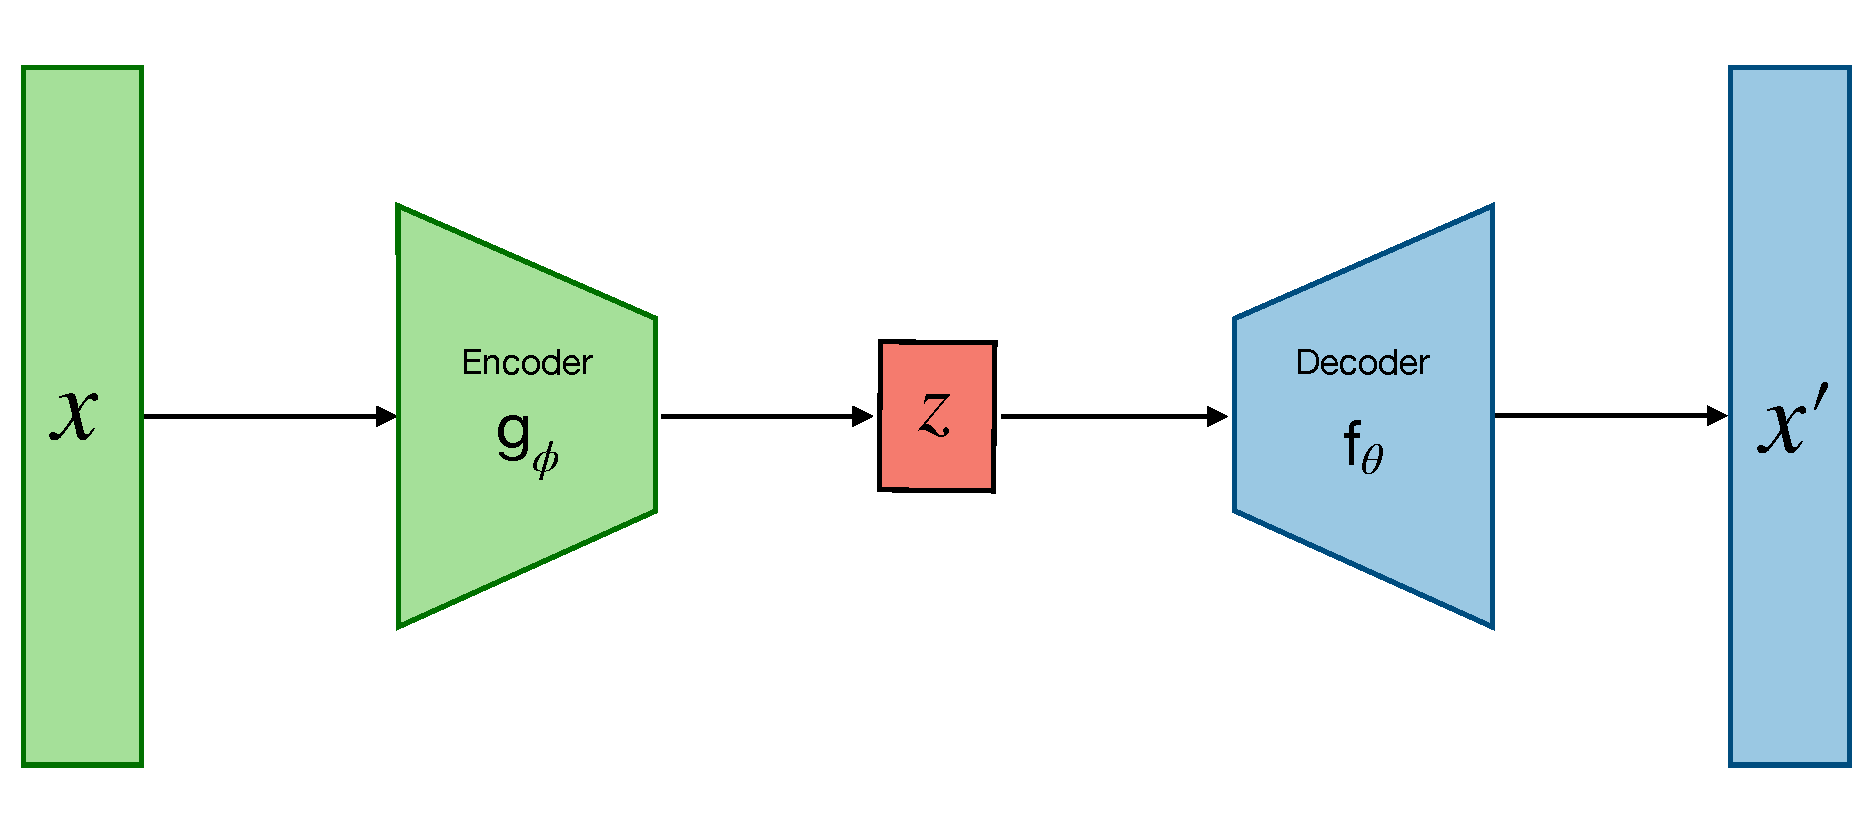
\includegraphics[width=\textwidth]{images/AE.pdf}
    \end{minipage}
    \hfill
    \begin{minipage}{0.7\textwidth}
        \centering
        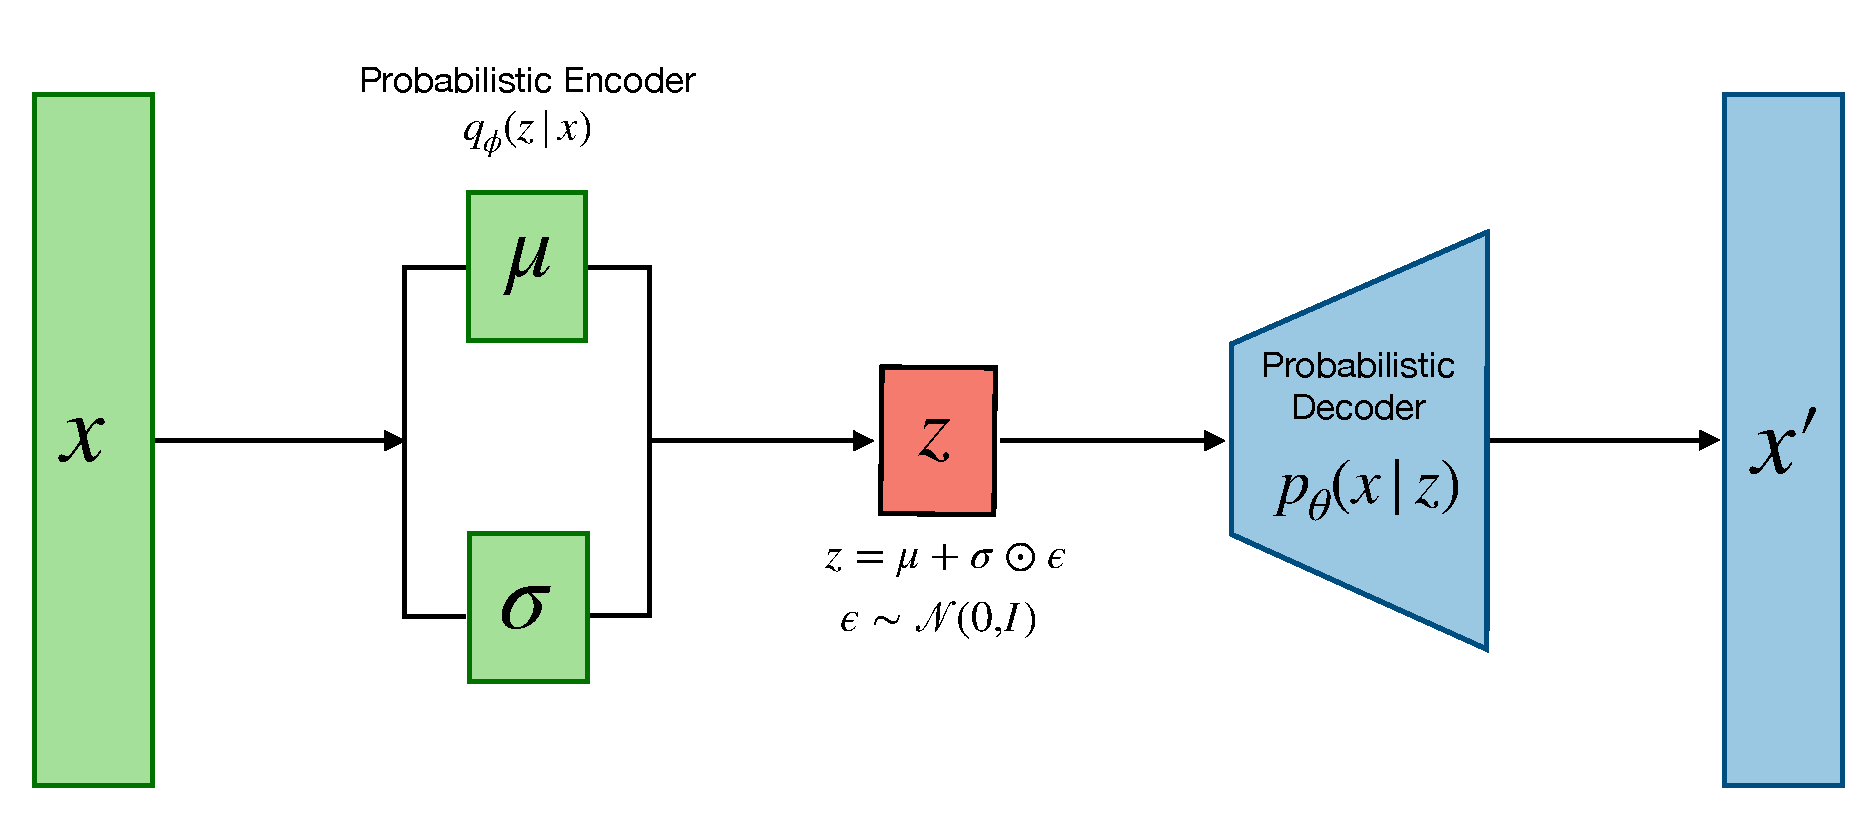
\includegraphics[width=\textwidth]{images/VAE.pdf}
    \end{minipage}
    \caption{Visual illustration of an Autoencoder (top) and a Variational Autoencoder (bottom). Inspired from 
    \cite{weng2018VAE}}
    \label{fig:AE_VAE}
\end{figure}


\subsection{Diffusion}
Diffusion models are a class of generative models that have gained significant attention 
for their ability to generate high-quality data (e.g., images, audio). These models 
operate by simulating two key processes: a forward diffusion process and a reverse 
denoising process.\newline
In the forward process, noise is gradually added to the data until it becomes indistinguishable
from a known distribution, typically Gaussian. The model then learns to reverse this process, 
step by step, denoising the data to recover samples that resemble those from the original dataset.\newline
A key difference between diffusion models and VAEs is that diffusion models operate through an iterative 
process, unlike VAEs which use a single step for encoding. Additionally, diffusion models 
do not reduce the dimensionality of the latent space and instead of learning the encoder they employ 
simple Gaussian noise as an encoder.
\vspace{-1cm}
\begin{figure}[H]
    \centering
    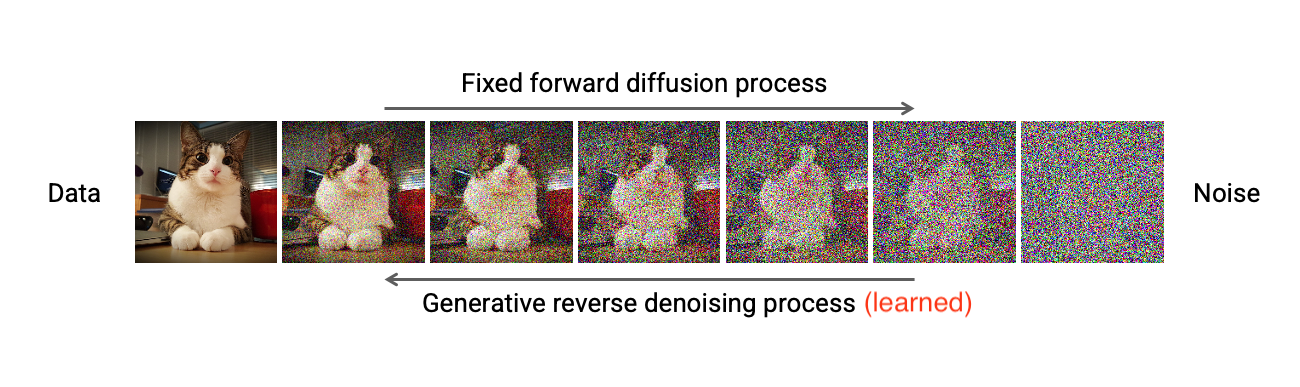
\includegraphics[width=1\linewidth]{images/diffusion.png}
    \caption{Illustration of the diffusion process}
    \label{fig:diffusion}
\end{figure}
The relationship between the data and latent variables in diffusion models is typically modeled as a Markov chain,
where each step depends only on the previous one.

\subsubsection{Forward Diffusion Process}
The forward diffusion process is a corruption process that takes a data sample (e.g., an 
image) and gradually adds noise to it in multiple steps, transforming the data into pure 
noise. This process can be described as follows:

\paragraph{Start with Data}
Start with an original data point $x_0$ (e.g., an image).

\paragraph{Add Noise in Steps}
At each time step $t$ noise is added to the previous state $z_{t-1}$ resulting in a more degraded version $z_t$. 
This process is modeled as a Markov chain:
\begin{align*}
    q(z_t | z_{t-1}) &= \mathcal{N}(z_t;\underset{\text{mean}}{\sqrt{1-\beta_t}z_{t-1}},\overset{\text{variance}}{\beta_tI}) \\
    &= \sqrt{1-\beta _t} z_{t-1} + \sqrt{\beta_t}\epsilon \sim \mathcal{N}(0,I) 
\end{align*}
We once again apply the reparameterization trick (see Section~\ref{reparametrization_trick}). 
To obtain $z_{100}$, the transformation would normally be applied sequentially over 100 steps. However, 
due to the properties of the Gaussian distribution, it is also possible to express this as a single-step
transformation from the original input. To do this, we define the following parameters:
$$\alpha_t = 1- \beta_t \qquad \bar{\alpha}_t = \prod_{s=1}^t\alpha_s$$ 
Here $\alpha_t$ defines the noise schedule, determining how much noise is added at each step. The one-step method can now be 
derived as follows:
\begin{align*}
    z_t &=  \sqrt{1-\beta _t} z_{t-1} + \sqrt{\beta_t} \epsilon \\
        &=  \sqrt{\alpha_t} {\color{cyan}z_{t-1}} + \sqrt{1-\alpha_t} \epsilon \\
        &=   \sqrt{\alpha_t} ({\color{cyan}\sqrt{\alpha_{t-1}} {\color{cyan}z_{t-2}} + \sqrt{1-\alpha_{t-1}} \epsilon}) + \sqrt{1-\alpha_t} \epsilon \numberthis \\
        &= \sqrt{\alpha_t \alpha_{t-1}}z_{t-2} +  
        \underbrace{\sqrt{\alpha_t-\alpha_t\alpha_{t-1}}\epsilon}_{\mathcal{N}(0,(\alpha_t-\alpha_t\alpha_{t-1})I)} + 
        \underbrace{\sqrt{1-\alpha_t} \epsilon}_{\mathcal{N}(0, (1-\alpha_t)I)} \\
        &=  \sqrt{\alpha_t \alpha_{t-1}}z_{t-2} + \sqrt{\alpha_t-\alpha_t\alpha_{t-1} + 1 - \alpha_t} \epsilon 
        &&(\text{sum of ind. gaussians \footnotemark})\\
        &= \sqrt{\alpha_{t}\alpha_{t-1}} z_{t-2} + \sqrt{1-\alpha_{t}\alpha_{t-1}}\epsilon \\
        &\vdots \quad (\text{repeat same steps from 14})\\
        &= \sqrt{\bar{\alpha}_t}z_0+\sqrt{1-\bar{\alpha}_t}\epsilon \\
        &\rightarrow q(z_t|z_0) = \mathcal{N}(z_t,\sqrt{\bar{\alpha}_t}z_0,\sqrt{1-\bar{\alpha}_t}I)
\end{align*}\footnotetext{Sum of two independent Gaussian variables $u \sim \mathcal{N}(\mu_u,\sigma_u^2)$ and 
$v \sim \mathcal{N}(\mu_v,\sigma_v^2)$ is a gaussian variable $ (u+v) \sim \mathcal{N}(\mu_u+\mu_v,\sigma_u^2+\sigma_v^2)$}

\subsubsection{Reverse Diffusion Process}
The reverse diffusion process is the key to generating new data points. It attempts to reverse the forward diffusion process 
and recover the original data from noise, essentially denoising the corrupted data step by step.
\paragraph{Start with Noise} The process starts with a noise sample, $z_t$, and iteratively denoises it by applying learned 
denoising steps.
\paragraph{Learned Model} The reverse process is learned by training a neural network to predict the denoised version 
of $z_t$ at each step $t$. Essentially, the model learns to reverse the noising process at each step meaning 
$p_\theta(z_{t-1}|z_t)$
\paragraph{Generate Data} By applying the reverse process step by step (starting from noise and gradually removing noise),
the model generates a new data sample that resembles the distribution of the original training data. The reverse process can 
be modelled as a parametrised Gaussian: 
$$p_\theta(z_{t-1}|z_t )= \mathcal{N}(z_{t-1};\mu_\theta(z_t,t),\Sigma_\theta(z_t,t))$$

\subsubsection{Training}
Training a diffusion model involves learning how to reverse the diffusion process. 
Specifically, the model is trained to predict the data at time step $t-1$ from the noisy 
data at time step $t$. This requires learning how to gradually denoise the data and 
requires a loss function that captures the reconstruction error over the multiple steps.
Diffusion models are trained using a likelihood-based approach, aiming to maximize the 
log-likelihood of the data. This is typically done through the Evidence Lower Bound (ELBO),
which incorporates various probabilistic components. A full derivation of this training objective
can be found in the original paper by Ho et al. \cite{ho2020denoisingdiffusionprobabilisticmodels}. 
The resulting bound is:
$$\log{p_\theta(x)} \geq \log{p_\theta(x|z_1)} - \overset{T}{\underset{t=2}{\sum}} \text{KL}(q(z_{t-1}|z_t,x)||p_\theta(z_{t-1}|z_t))-\text{KL}(q(z_T|x)||p(z_T))$$
This can be further simplified since the last term does not depend on the parameters 
$\theta$. Additionally, we know that $p_\theta(z_{t-1}|z_t)$  is the Gaussian we want to 
learn, and it turns out that  $q(z_{t-1}|z_t,x)$ is also a Gaussian. 
Therefore, we can use the closed-form KL divergence between two Gaussians. 

%\begin{figure}[H]
%\begin{minipage}[t]{0.495\textwidth}
%\begin{algorithm}[H]
%  \caption{Training} \label{alg:training}
%  \small
%  \begin{algorithmic}[1]
%    \REPEAT
%      \STATE $x_0 \sim q(x_0)$
%      \STATE $t \sim \mathrm{Uniform}(\{1, \dotsc, T\})$
%      \STATE $\epsilon\sim\mathcal{N}(0,I)$
%      \STATE Take gradient descent step on
%      \STATE $\qquad \nabla_\theta \left\| \epsilon - \epsilon_\theta(\sqrt{\bar\alpha_t} x_0 + \sqrt{1-\bar\alpha_t}\epsilon, t) \right\|^2$
%    \UNTIL{converged}
%  \end{algorithmic}
%\end{algorithm}
%\end{minipage}
%\hfill
%\begin{minipage}[t]{0.495\textwidth}
%\begin{algorithm}[H]
%%  \caption{Sampling} \label{alg:sampling}
%  \small
%  \begin{algorithmic}[1]
%    \vspace{.04in}
%    \STATE $x_T \sim \mathcal{N}(0, I)$
%    \FOR{$t=T, \dotsc, 1$}
%      \STATE $z \sim \mathcal{N}(0, I)$ if $t > 1$, else $z = 0$
%      \STATE $x_{t-1} = \frac{1}{\sqrt{\alpha_t}}\left( x_t - \frac{1-\alpha_t}{\sqrt{1-\bar\alpha_t}} \epsilon_\theta(x_t, t) \right) + \sigma_t z$
%    \ENDFOR
%    \STATE \textbf{return} $x_0$
%    \vspace{.04in}
%  \end{algorithmic}
%\end{algorithm}
%\end{minipage}
%\vspace{-1em}
%\end{figure}

\subsection{Score-Based Generative Models}
Score-based generative models \cite{song2021scorebasedgenerativemodelingstochastic} are a class of models that learn
the score function of a data distribution — the gradient of the log-probability density with respect to the data:
$$\nabla_x \log{p(x)}$$
As with other generative models, the goal is to learn the data distribution $p_\theta(x)$ and generate new samples from it.
A common formulation expresses the data distribution as:
$$p_\theta(x) = \frac{e^{-f_\theta(x)}}{Z_\theta}$$
However, the problem with this direct approach is that it requires knowledge of the 
normalization constant $Z_\theta$, which involves solving an integral over the entire 
domain, a task that is often intractable. By instead taking the gradient of the log-probability, we get:
$$\nabla_x \log{p_\theta(x)} = \nabla_x \log{e^{-f_\theta(x)}}-\nabla_x \log{Z_\theta}=- \nabla_x f_\theta(x)$$
This is the core insight of score-based models: instead of modeling $p_\theta(x)$ directly, we model how the probability 
density changes in space. Once the score function is learned, we can generate samples by following these gradients in a 
stochastic manner (e.g., via Langevin dynamics).

\subsection{Flow Matching}
Flow matching \cite{lipman2023flowmatchinggenerativemodeling} is a method for training generative models based on 
the idea of aligning data distributions through normalizing flows. A normalizing flow is a series of invertible
transformations applied to a simple distribution (e.g., a Gaussian) to model complex data distributions.\newline
Flow matching introduces a novel way of training generative models by matching the gradients of the data density 
at different stages of the transformation. This is done by learning the flow that transforms a simple distribution 
(like Gaussian noise) into a more complex data distribution.
Really helpful resource can be found \href{https://www.youtube.com/watch?v=7cMzfkWFWhI}{here}


\subsection{Connecting Diffusion Models and Reinforcement Learning}
An interesting connection exists between diffusion models and reinforcement learning (RL): diffusion models can be used to 
generate new plausible policies that resemble those from the original dataset. In other words, instead of learning from the 
dataset directly, we learn a distribution over good trajectories (or policies), and then sample new ones using diffusion 
processes. This perspective opens up new possibilities in offline RL and imitation learning, where the goal is to generalize 
and generate diverse, high-performing behaviors from limited data.

\subsection{Resources}
In this section, we did not delve into the full mathematical derivations behind the various generative modeling approaches, as 
these tend to be quite lengthy. For readers interested in the detailed math, I recommend reading the original papers. 
Additionally, there are some excellent resources that explain these concepts more intuitively. A great video series covering 
diffusion models, score-based diffusion models, and flow matching can be found here \cite{outlier}. Lilian Weng’s blog post "What 
Are Diffusion Models?" \cite{weng2021diffusion} is also very well written and highly recommended. For a deeper understanding of 
score-based models, Yang Song’s blog \cite{YangSong} is one of the best resources available. A particularly insightful paper that 
highlights the connections between the various generative modeling approaches discussed is \cite{luo2022understandingdiffusionmodelsunified}.


\section{Distributional Reinforcement Learning}
Distributional Reinforcement Learning (DRL) is an extension of traditional reinforcement 
learning (RL) that focuses on modeling the distribution of return values (rewards) rather 
than just predicting the expected return.\newline
In traditional RL, the goal is often to maximise the expected cumulative reward (value function) for a given state . $$V ^\pi(s) = \mathbb{E}_\pi\left[\sum_{k=0}^\infty\gamma^k r_{t+1+k}|s_t=s\right]$$
However, in distributional reinforcement learning, instead of focusing on a single expected 
value, we learn the full distribution of the returns. This means that, instead of predicting 
just the expected return (like a scalar value), we model the entire range of possible future 
rewards and their probabilities. \newline
Imagine you're playing a video game where, at some points, you can make a risky move that 
might either yield a high reward or result in a penalty. In traditional RL, you might expect 
the average reward (e.g., 5 points), but in distributional RL, you can learn the probability 
distribution of rewards—e.g., 70\% chance for +10 points, 20\% chance for +5 points, and 
10\% chance for -5 points. This distributional approach helps the agent better weigh its 
decisions.

\subsection{Resources}
The content presented here is intended as a brief overview and will be expanded and improved in the future. For a deeper 
understanding, a highly recommended lecture is ''Deep RL Bootcamp Frontiers Lecture I: Recent Advances, Frontiers, and 
Future of Deep RL`` \cite{DeepRlBootcamp}.





%\section{Motion Primitives}
Motion Primitives (MPs) are a way to represent and control robot movements in reinforcement 
learning (RL). MPs are like pre-designed building blocks for smooth, efficient robot 
trajectories (paths or motions). Imagine you’re teaching a robot to move its arm smoothly 
from point A to point B. Instead of telling it every tiny step ("move 1cm, then 2cm, then 
turn..."), you give it a single, smooth "recipe" for the whole motion. Desired trajectory 
$\tau$ is generated using parameters $\omega$  of the MP and initial conditions of the agent 
(joint position $y_0$  and velocity  $\dot{y}_0$). 

\subsection{Dynamic Motion Primitives (DMPs)}
One can think of DMPs as a system with a "moving target" (called an attractor). The robot’s 
motion is guided by a simple equation that pulls it toward a goal while adding a 
customizable "force" to shape the path.
$$\ddot{y} = \alpha(\beta(\underbrace{g+\frac{f_\omega(t)}{\alpha\beta}}_{\text{Moving Attractor}}-y)-\dot{y})$$
The forcing function $f_\omega(t)$ (learnable) encodes the desired additional acceleration profile.  
\begin{itemize}
    \item Pros: \begin{itemize}
        \item Smooth trajectories (no jerkiness).
        \item Stable by design (won’t go wild).
        \item Easy to tweak speed or end position.
    \end{itemize}
    \item Cons: Hard to capture complex variations in motion.
\end{itemize}

\subsection{Probabilistic Motion Primitives (ProMPs)}
ProMPs use a set of basic shapes (basis functions) to draw the trajectory directly, plus a 
probability model to account for uncertainty or variation (e.g., "this motion might vary a 
bit").
\begin{itemize}
    \item Pros:\begin{itemize}
        \item Can adapt to specific points (e.g., "pass through here at time X").
        \item Models variations well (useful for human-robot teamwork).
    \end{itemize}
    \item Cons: Replanning mid-motion can cause jumps (not smooth).
\end{itemize}

\subsection{Probabilistic Dynamic Motion Primitives (ProDMPs)}
ProDMPs blend DMPs and ProMPs. They solve the DMP equations to keep smoothness and add 
ProMP’s probabilistic flexibility.
\begin{itemize}
    \item Pros: \begin{itemize}
        \item Smooth even when replanning.
        \item Handles variations and adapts to new conditions.
    \end{itemize}
    \item Cons: A bit more complex to set up.
\end{itemize}


\bibliographystyle{alpha}
\bibliography{sample}

\end{document}